% !TEX program = xelatex
\documentclass[UTF8,a4paper,11pt,fontset=windows]{ctexart}
\usepackage[margin=2.15cm]{geometry}
\usepackage{amsmath,amssymb,amsthm,enumitem,booktabs,longtable,array,graphicx,tikz,fancyhdr}
\usepackage[unicode,hidelinks]{hyperref}
\allowdisplaybreaks[2]
\setlength{\headheight}{15pt}
\pagestyle{fancy}\fancyhf{}\fancyhead[L]{常微分方程期末复习}\fancyhead[R]{前五章习题与求解方法}\fancyfoot[C]{\thepage}
\setlength{\parskip}{0.35em}\setlength{\emergencystretch}{2em}
\setlist[enumerate]{itemsep=0.35em,topsep=0.4em}
\setcounter{tocdepth}{2}
\newcommand{\dd}{\mathrm d}\newcommand{\R}{\mathbb R}\newcommand{\e}{\mathrm e}\newcommand{\ii}{\mathrm i}
\newcommand{\problem}[3]{\subsection{习题 #1}\label{q:#1}\noindent\textbf{题目}\quad #3\par\noindent{\small 教材印刷页 #2；扫描 PDF 页码加 10。}\par\smallskip}
\newcommand{\method}[1]{\par\noindent\textbf{方法}\quad #1\par}
\newcommand{\ans}[1]{\par\noindent\textbf{标准答案}\[\boxed{\begin{gathered}#1\end{gathered}}\]}
\newcommand{\checknote}[1]{\par\noindent{\small\textbf{核对}\quad #1}\par}
\newcommand{\basis}[1]{\par\noindent{\small\textbf{知识点依据}\quad #1}\par}
\renewcommand{\proofname}{证明}
\title{常微分方程期末复习\\\large 张伟年、杜正东、徐冰《常微分方程》第2版\\前五章计算题全解与指定理论题}
\author{}\date{2026年11月24日}
\begin{document}\maketitle
本册计算题覆盖教材前五章各节习题中的全部计算小问，包括建模、消去常数、求通解与初值解、积分因子、奇解、降阶、线性方程组、级数、Picard 迭代、数值计算及解对初值的导数。其余理论题按所提供课堂照片选取。题目沿用第二版编号；每题列出所需条件、计算步骤和结果。

照片中的“习题2.3（第三版）1、2”不能按题号直接移植：所供第二版第2.3节没有单列习题，相关隐式方程计算集中于习题2.4，本册已全部收入。没有取得第三版题面，因此不声称已核对两版这两道题的一一对应关系。

常数在各题、各小问中独立使用。通解默认在使原方程及所写表达式有意义的连通开区间上取值；除法前另行检查被除因子的零点。隐式解需要选取可微函数分支，不能把整条代数曲线都视为一条函数解。理论题证明为依据教材本节方法所作的完整推导，不声称教材提供了原题证明。
\tableofcontents\clearpage
\section{求解方法与选法顺序}
\subsection{先检查什么}
先明确自变量、未知函数、阶数、初值和定义域。求解后检查原方程、初值、被除去的因子及最大存在区间。求一阶显式方程时，依次检查能否直接积分、分离变量、化为齐次方程、一阶线性方程、Bernoulli 方程或恰当方程；导数没有解出时，再检查可否解出 $y$、解出 $x$、因式分解或参数化。高阶方程先检查缺项降阶，再检查线性结构。
\subsection{分离变量与可化为分离变量的方程}
\basis{第2.1节，教材第15--27页。}
对 $y'=h(x)g(y)$，先记录每个 $g(a)=0$ 给出的常值解 $y=a$，再在 $g(y)\ne0$ 的区间上积分：
\[
 \int\dfrac{\dd y}{g(y)}=\int h(x)\,\dd x+C.
\]
若 $y'=F(y/x)$，令 $y=xu$，则
\[
 y'=u+xu',\qquad xu'=F(u)-u.
\]
先检查 $F(u)-u=0$ 对应的直线解，再分离变量。
对线性分式 $y'=F((a_1x+b_1y+c_1)/(a_2x+b_2y+c_2))$，两直线相交时平移交点为原点；两组系数成比例时，用 $u=ax+by$。对 $y'=F(ax+by+c)$，同样令 $u=ax+by+c$，得到 $u'=a+bF(u)$。
\subsection{一阶线性、反置变量与 Bernoulli 方程}
\basis{第2.1节，第17--22页。}
对 $y'+p(x)y=q(x)$，乘积分因子 $\mu=\exp(\displaystyle\int p(x)\,\dd x)$，得
\[
 (\mu y)'=\mu q,\qquad y=\mu^{-1}\left(C+\int\mu q\,\dd x\right).
\]
若方程关于 $y(x)$ 非线性而关于 $x(y)$ 线性，交换自变量与因变量。反置过程只能用于导数非零的分支，另查常值解。

对 $y'=a(x)y+b(x)y^\alpha$，$\alpha\ne0,1$，在非零分支令 $z=y^{1-\alpha}$：
\[
 z'=(1-\alpha)a(x)z+(1-\alpha)b(x).
\]
当分数幂出现时，回代必须满足原有符号条件；平方后的式子可能增加伪解。
\subsection{恰当方程与积分因子}
\basis{第2.2节，第27--37页。}
对 $M\,\dd x+N\,\dd y=0$，在适当的单连通区域检查 $M_y=N_x$。若成立，先积分 $F=\displaystyle\int M\,\dd x+g(y)$，再用 $F_y=N$ 求 $g$，解为 $F=C$。
若不恰当，检查
\[
 \dfrac{M_y-N_x}{N}=f(x)\Rightarrow\mu(x)=\e^{\int f(x)\,\dd x},\qquad
 \dfrac{N_x-M_y}{M}=g(y)\Rightarrow\mu(y)=\e^{\int g(y)\,\dd y}.
\]
若 $M,N$ 同次齐次且 $xM+yN\ne0$，可试 $\mu=(xM+yN)^{-1}$。找不到上述形式时可试 $x^ay^b$，代入 $(\mu M)_y=(\mu N)_x$ 比较系数。积分因子不应在所取区域为零；其奇点处的原方程解需另查。
\subsection{隐式一阶方程、参数法和奇解}
\basis{第2.3--2.4节，第37--49页。}
记 $p=y'$。若 $y=f(x,p)$，求微分后得到
\[
 p=f_x+f_p\dfrac{\dd p}{\dd x}.
\]
若便于求 $x(p)$，改写为它的一阶方程，再由 $y=f(x(p),p)$ 回代。若 $y=xp+f(p)$ 是 Clairaut 方程，则
\[
 (x+f'(p))p'=0.
\]
$p=C$ 给出直线族，$x=-f'(p),\ y=f(p)-pf'(p)$ 给出包络候选。必须代回原方程验证，才能确认为奇解。一般 $F(x,y,p)=0$ 的 $p$ 判别曲线由 $F=F_p=0$ 得到，也只给出候选。
若可解出 $x=f(y,p)$，则由 $\dd x=f_y\dd y+f_p\dd p$、$\dd y=p\dd x$ 得
\[
 (1-pf_y)\dd y=pf_p\dd p.
\]
将 $y$ 视为 $p$ 的函数求解，再回代求 $x$。若方程只含 $x,p$，先求出 $p$ 的分支，再积分 $y'=p(x)$；若只含 $y,p$，可先求 $p(y)$，再用 $\dd x=\dd y/p(y)$。

Lagrange 方程 $y=x\phi(p)+\psi(p)$ 求导后为
\[
 p-\phi(p)=[x\phi'(p)+\psi'(p)]\dfrac{\dd p}{\dd x}.
\]
在 $p\ne\phi(p)$ 的分支上，反置为线性方程
\[
 \dfrac{\dd x}{\dd p}-\dfrac{\phi'(p)}{p-\phi(p)}x
 =\dfrac{\psi'(p)}{p-\phi(p)}.
\]
解出 $x(p)$ 后由原式给出 $y(p)$；每个 $p_0=\phi(p_0)$ 还给出直线候选 $y=p_0x+\psi(p_0)$，应直接回代。Clairaut 方程是 $\phi(p)=p$ 的特殊情形，不能用上式除以恒为零的分母。
\subsection{高阶非线性方程降阶}
\basis{第2.4节，第49--54页。}
缺 $y$ 时令 $p=y'$；缺 $x$ 时在非恒定分支令 $p=p(y)$，用 $y''=p\,\dd p/\dd y$。若出现 $yy''-(y')^2$，用
\[
 \left(\dfrac{y'}y\right)'=\dfrac{yy''-(y')^2}{y^2}.
\]
出现连续高阶导数时，也可先把最高的共同低阶导数作为新未知函数。降阶后每积分一次都应加入一个独立常数，并另查除法遗漏的常值解。
\subsection{Riccati 方程的已知特解法}
\basis{第2.4节，第54--57页。}
对 $y'=a(x)y^2+b(x)y+c(x)$，若已知一个特解 $y_1$，令 $z=y-y_1$，利用 $y_1$ 满足原方程，得到
\[
 z'=(2ay_1+b)z+az^2.
\]
$z=0$ 就是已知特解；对 $z\ne0$ 令 $u=1/z$，化成
\[
 u'+(2ay_1+b)u=-a,\qquad y=y_1+\dfrac1u.
\]
若没有已知特解，一般不能保证用初等积分求解。不能因为方程是一阶就强行寻找初等闭式；可转用级数、Picard 迭代或数值法。
\subsection{变系数线性方程与方程组}
\basis{第3.2--3.4节，第65--80页。}
已知基本解矩阵 $X$ 时，齐次通解 $x=Xc$，非齐次解为
\[
 x(t)=X(t)\left[X^{-1}(t_0)x_0+\int_{t_0}^tX^{-1}(s)f(s)\,\dd s\right].
\]
若已知二阶齐次方程 $y''+a_1y'+a_2y=0$ 的非零解 $y_1$，令 $y=y_1u$，得
\[
 y_1u''+(2y_1'+a_1y_1)u'=0,
 \qquad y_2=y_1\int\dfrac{\e^{-\int a_1\,\dd t}}{y_1^2}\,\dd t.
\]
$y_1$ 的零点处可分区间计算，再用原方程的唯一性拼接。二阶非齐次方程可用常数变易：设 $y=c_1(t)y_1+c_2(t)y_2$，联立
\[
 c_1'y_1+c_2'y_2=0,\qquad c_1'y_1'+c_2'y_2'=f.
\]
\subsection{常系数线性方程：特征根与待定系数}
\basis{第4.1--4.2节，第90--99页。}
把 $D=\dd/\dd t$ 代入多项式 $P(D)$。特征根 $\lambda$ 的重数为 $m$ 时，贡献 $\e^{\lambda t},t\e^{\lambda t},\ldots,t^{m-1}\e^{\lambda t}$；共轭根 $\alpha\pm\ii\beta$ 的重数为 $m$ 时，取相应的实部和虚部。

右端为 $\e^{\alpha t}Q_k(t)$ 时，试 $t^s\e^{\alpha t}R_k(t)$，其中 $s$ 为 $\alpha$ 的重数；右端有 $\cos\beta t$ 或 $\sin\beta t$ 时，可将 $\alpha$ 换成 $\alpha+\ii\beta$ 取实部或虚部。代入原方程比较系数。最后加齐次通解。

算子移位公式为
\[
 P(D)(\e^{\alpha t}u)=\e^{\alpha t}P(D+\alpha)u.
\]
对多项式右端的 $P(D)^{-1}$ 展开在有限次求导后终止；$D^{-1}$ 代表积分，积分常数统一收入齐次解。对一般右端可用常数变易，不把形式逆算子当成普通数分式。
Cauchy--Euler 方程在 $t>0$ 或 $t<0$ 上令 $s=\ln|t|$，则
\[
 ty'=u_s,\qquad t^2y''=u_{ss}-u_s.
\]
\subsection{常系数方程组：特征向量、Jordan 链与消元}
\basis{第4.3节，第99--108页。}
对 $x'=Ax$，先求 $\det(\lambda I-A)$。每个特征向量 $v$ 给出 $\e^{\lambda t}v$。若 $(A-\lambda I)v_1=v_0$，则第二个解为 $\e^{\lambda t}(v_1+tv_0)$。长度三的链再给出 $\e^{\lambda t}(v_2+tv_1+t^2v_0/2)$。用 $Av_0=\lambda v_0$ 和链关系逐一核验，不能只看特征值。

也可先消元求某一分量，再从原方程恢复其余分量。算子行列式消元给出的标量方程是必要条件；各分量积分常数必须回代原组建立关系。
\subsection{幂级数法和 Frobenius 法}
\basis{第3.5节，第80--87页。}
在普通点 $t_0$ 令 $y=\sum_{n\ge0}a_n(t-t_0)^n$，求导、统一幂次、逐项比较，写出递推及首项。普通点到最近复奇点的距离给出至少可保证的收敛半径，整系数的首项系数恒不为零时解可为整函数。
正则奇点可试 $y=(t-t_0)^r\sum_{n\ge0}a_n(t-t_0)^n$，先由最低次项求指标方程，再求递推；重根或根差为整数时可能需要对数项。多项式解来自递推在某一项终止。

例如教材的 Bessel 型方程 $t^2y''+ty'+(t^2-\nu^2)y=0$，取 $t>0$，令 $y=t^r\sum_{n\ge0}a_nt^n$、$a_0\ne0$。最低次项给出指标方程 $r^2-\nu^2=0$，其余系数满足
\[
 [(r+n)^2-\nu^2]a_n=-a_{n-2},\qquad a_{-1}=a_{-2}=0.
\]
选择一个指标根后，先查每一步分母是否为零，再递推；若分母为零，应检查兼容性并另求第二解，不能继续作除法。
\subsection{Picard 迭代、存在区间与误差}
\basis{第5.1节，第115--122页。}
在 $|t-t_0|\le a,|x-x_0|\le b$ 上，取 $M=\max|f|$ 及关于 $x$ 的 Lipschitz 常数 $L$，令 $h=\min(a,b/M)$。$M=0$ 时可取 $h=a$。迭代为
\[
 \varphi_0=x_0,\qquad\varphi_{n+1}(t)=x_0+\int_{t_0}^tf(s,\varphi_n(s))\,\dd s.
\]
误差满足
\[
 |\varphi_n-\varphi|\le\dfrac{ML^n|t-t_0|^{n+1}}{(n+1)!}.
\]
由此选择最小足够的 $n$；局部定理给出的区间不能直接当成最大存在区间。最大区间要检查显式解的奇点、原方程定义域，或使用延拓定理。
\subsection{数值方法、比较估计和参数导数}
\basis{第5.2、5.4--5.6节，第122--129、136--159页。}
Euler 法：$x_{n+1}=x_n+hf(t_n,x_n)$。改进 Euler 法（显式梯形法）先预测，再校正：
\[
 \widetilde x_{n+1}=x_n+hf(t_n,x_n),\qquad
 x_{n+1}=x_n+\dfrac h2[f(t_n,x_n)+f(t_n+h,\widetilde x_{n+1})].
\]
四阶 Runge--Kutta 法：
\[
 \begin{aligned}
 K_1&=f(t_n,x_n),&K_2&=f(t_n+h/2,x_n+hK_1/2),\\
 K_3&=f(t_n+h/2,x_n+hK_2/2),&K_4&=f(t_n+h,x_n+hK_3),\\
 x_{n+1}&=x_n+\dfrac h6(K_1+2K_2+2K_3+K_4).
 \end{aligned}
\]
若满足足够光滑性，在固定有限区间上三者全局误差分别为 $O(h),O(h^2),O(h^4)$。反向计算时步长取负，仍从给定初值出发，不能把左端点误作初值点。

对 $u(t)\le c+\displaystyle\int_{t_0}^ta(s)u(s)\,\dd s$，$a\ge0$，Gronwall 估计为 $u(t)\le c\exp(\displaystyle\int_{t_0}^ta(s)\,\dd s)$。由积分式取差、取模，再应用该估计可处理近似解误差与初值敏感性。

若 $x=\varphi(t;t_0,x_0,\mu)$，则变分方程为
\[
 U'=f_xU,\ U(t_0)=I;\qquad V'=f_xV+f_\mu,\ V(t_0)=0;
 \qquad \varphi_{t_0}=-U(t)f(t_0,x_0,\mu).
\]
先代入所讨论的基准解，再解这个线性方程，通常比先求非线性通解简单。

\clearpage\section{第一章：绪论}
\problem{1.1.1}{6}{船以相对水流恒定速度 $v_0$ 垂直向对岸行驶。水流沿河岸方向，速率与船到两岸的距离乘积成正比，比例系数 $k$，河宽 $a$。求轨迹满足的微分方程。}
取 $x$ 轴沿水流方向，$y$ 轴垂直河岸，出发岸为 $y=0$、对岸为 $y=a$。船在横渡位置 $y$ 时到两岸的距离分别为 $y$ 和 $a-y$，所以当地水流速度为 $ky(a-y)$。

船相对于水的速度为 $(0,v_0)$，水相对于河岸的速度为 $(ky(a-y),0)$。两者相加得到船相对于河岸的速度：
\[
\dfrac{\dd x}{\dd t}=ky(a-y),\qquad \dfrac{\dd y}{\dd t}=v_0.
\]
因 $v_0>0$，可用第二式消去时间：
\[
\begin{aligned}
\dfrac{\dd x}{\dd y}&=\dfrac{\dd x/\dd t}{\dd y/\dd t}
=\dfrac{k}{v_0}(ay-y^2),\\
x(y)-x(0)&=\dfrac{k}{v_0}\int_0^y(a\eta-\eta^2)\dd\eta\\
&=\dfrac{k}{v_0}\left(\dfrac{ay^2}{2}-\dfrac{y^3}{3}\right).
\end{aligned}
\]
令出发点沿岸坐标 $x(0)=x_0$，便得轨迹公式。
\ans{\dfrac{\dd x}{\dd y}=\dfrac{k}{v_0}y(a-y),\qquad
x-x_0=\dfrac{k}{v_0}\left(\dfrac{ay^2}{2}-\dfrac{y^3}{3}\right).}
这里 $y=v_0t$（出发时刻取零）。到岸时间 $a/v_0$，漂移 $ka^3/(6v_0)$。
\checknote{轨迹求导恢复速度比；$k=0$ 时轨迹垂直河岸，量纲与渡河时间一致。}
\problem{1.1.2}{6}{求平面曲线满足的微分方程，使各点处切线、该点向径和 $Ox$ 轴构成等腰三角形。}
原题没有指定哪两边为腰，故应分别讨论三种构型。设 $O=(0,0)$、切点 $P=(x,y)$，切线与横轴交于 $T=(a,0)$，三角形非退化。三条边的平方为
\[
OP^2=x^2+y^2,\quad PT^2=(x-a)^2+y^2,\quad OT^2=a^2.
\]
记切线斜率 $p=y'$，由两点斜率公式 $p=y/(x-a)$，即 $(x-a)p=y$。
\begin{enumerate}
\item $OP=PT$ 时，$x^2=(x-a)^2$，展开得 $a(a-2x)=0$。$a=0$ 会使 $T=O$、三角形退化，故取 $a=2x$。代入切线式有 $-xp=y$。
\item $OP=OT$ 时，$a^2=x^2+y^2$，所以 $a=\pm\sqrt{x^2+y^2}$，代入 $(x-a)p=y$ 即得相应两种朝向的方程。
\item $OT=PT$ 时，$a^2=x^2-2ax+a^2+y^2$，即 $2ax=x^2+y^2$。在非退化构型中 $x\ne0$，故 $a=(x^2+y^2)/(2x)$。代回切线式并乘 $2x$，得到 $(x^2-y^2)p=2xy$。
\end{enumerate}
\ans{OP=PT:\ xy'+y=0;\qquad OP=OT:\ (x\mp\sqrt{x^2+y^2})y'=y;\\
OT=PT:\ (x^2-y^2)y'=2xy.}
竖直切线处用相应微分形式解释。若课堂约定切线段与向径为两腰，则取第一式，积分为 $xy=C$。
\checknote{将各式对应的截距代入三条边长，分别恢复所要求的等长关系。}
\problem{1.2.1}{11}{证明 $x(t)=C\e^{-3t}+2t+1$ 为 $x'+3x=6t+5$ 的解，并求满足 $x(0)=3$ 的解。}
先对题给函数逐项求导，再代入方程左端：
\[
\begin{aligned}
x'&=-3C\e^{-3t}+2,\\
x'+3x&=(-3C\e^{-3t}+2)+3(C\e^{-3t}+2t+1)\\
&=-3C\e^{-3t}+3C\e^{-3t}+2+6t+3\\
&=6t+5.
\end{aligned}
\]
其中含任意常数的两项恰好抵消，故任意 $C$ 都给出解。最后由初值 $x(0)=C+1=3$ 得 $C=2$，将这个值代入函数族。
\ans{x(t)=2\e^{-3t}+2t+1.}
\checknote{代入方程及 $t=0$ 均满足要求，定义域为 $\R$。}
\problem{1.2.2}{12}{放射性物质镭的衰变速率与存余量成正比，比例系数 $k$。已知 $R(t_0)=R_0$，求 $R(t)$。}
“衰变速率与存余量成正比”表示 $-R'=kR$，其中 $k>0$，负号反映质量随时间减少。若 $R_0>0$，采用带初值的定积分分离变量：
\[
\begin{aligned}
\dfrac{\dd R}{R}&=-k\dd t,\\
\int_{R_0}^{R(t)}\dfrac{\dd r}{r}&=-k\int_{t_0}^t\dd s,\\
\ln\dfrac{R(t)}{R_0}&=-k(t-t_0).
\end{aligned}
\]
两端取指数，得到质量随时间的变化。若 $R_0=0$，原方程的零解满足初值，且线性方程的唯一性保证没有其他初值解。
\ans{R(t)=R_0\e^{-k(t-t_0)}.}
\checknote{初值正确，$R'=-kR$；$R_0\ge0$ 时质量非负并随时间不增。}
\problem{1.2.3}{12}{物体以初速度 $v_0$ 在空气中竖直上抛，质量 $m$，阻力大小为 $k^2v^2$。求运动规律及到达最高点的时间。}
取向上为正，$s(0)=s_0$，$v=s'$。上升时 $v\ge0$，重力和阻力都向下，所以 $mv'=-mg-k^2v^2$。记 $V=\sqrt{mg}/k$，则
\[
\begin{aligned}
\dfrac{\dd v}{1+(v/V)^2}&=-g\dd t,\\
V\left[\arctan\dfrac vV-\arctan\dfrac{v_0}{V}\right]&=-gt.
\end{aligned}
\]
令 $\omega=g/V=k\sqrt{g/m}$、$\theta=\arctan(v_0/V)$，得 $v=V\tan(\theta-\omega t)$。再积分求位置，使用 $\displaystyle \int\tan u\dd u=-\ln|\cos u|$：
\[
\begin{aligned}
s(t)-s_0&=\int_0^t V\tan(\theta-\omega\tau)\dd\tau\\
&=\dfrac V\omega\ln\dfrac{\cos(\theta-\omega t)}{\cos\theta}
=\dfrac m{k^2}\ln\dfrac{\cos(\theta-\omega t)}{\cos\theta}.
\end{aligned}
\]
最高点由 $v(t_*)=0$ 给 $t_*=\theta/\omega$；又 $1/\cos\theta=\sqrt{1+(v_0/V)^2}$，代入位置式得到 $s_*$。

下降时 $v<0$，阻力向上，故改用 $mv'=-mg+k^2v^2$。令 $w=-v/V$、$\tau=t-t_*$，则 $w'=\omega(1-w^2),w(0)=0$。分离积分给
\[
\dfrac12\ln\dfrac{1+w}{1-w}=\omega\tau,
\quad w=\tanh(\omega\tau).
\]
因此 $v=-V\tanh(\omega\tau)$，再由 $\displaystyle \int\tanh u\dd u=\ln\cosh u$ 积分得到下降位置。
\ans{v=V\tan(\theta-\omega t),\quad 0\le t\le t_*;\qquad t_*=\dfrac1\omega\arctan\dfrac{kv_0}{\sqrt{mg}},\\
s_*=s_0+\dfrac m{2k^2}\ln\left(1+\dfrac{k^2v_0^2}{mg}\right),\\
v=-V\tanh[\omega(t-t_*)],\quad
s=s_*-\dfrac m{k^2}\ln\cosh[\omega(t-t_*)]\quad(t\ge t_*).}
下降公式使用至触地时。$k=0$ 的情形取极限，得到 $s=s_0+v_0t-gt^2/2$、$t_*=v_0/g$。
\checknote{各阶段求导恢复正确方向的阻力；最高点位置与速度连续，$k\to0$ 恢复无阻力公式。}
\problem{1.2.4}{12}{将例1.2和例1.3的方程化为规范的一阶方程组。}
把二阶未知函数与其一阶导数分别作为两个新未知函数。
\begin{enumerate}
\item 单摆原式为 $\theta''=-(g/l)\sin\theta$。令 $u=\theta,v=\theta'$，则 $u'=\theta'=v$，$v'=\theta''=-(g/l)\sin u$。
\item 弹簧原式为 $mx''+\mu x'+kx=0$，先将最高阶导数解出：$x''=-(\mu/m)x'-(k/m)x$。再令 $u=x,v=x'$，得到 $u'=v$ 与 $v'=-(\mu/m)v-(k/m)u$。
\end{enumerate}
二阶初值 $x(t_0),x'(t_0)$ 分别转为 $u(t_0),v(t_0)$，没有增加也没有丢失初始数据。
\ans{\text{单摆：}\ \begin{cases}u'=v,\\v'=-(g/l)\sin u;\end{cases}\qquad
\text{弹簧：}\ \begin{cases}u'=v,\\v'=-(k/m)u-(\mu/m)v.\end{cases}}
\checknote{对第一式再求导并用第二式消去 $v$，分别恢复两个二阶方程；两个初值也一一对应。}
\problem{1.2.5(1)}{12}{作 $x'=|x|$ 的方向场，画出经过 $(0,0),(0,-1)$ 的积分曲线。}
按未知函数的符号把绝对值展开：
\[
x'=\begin{cases}x,&x>0,\\-x,&x<0,\\0,&x=0.\end{cases}
\]
因此正半平面上分离得 $\ln x=t+C_0$，解为 $x=C\e^t,C>0$；负半平面上有 $\dd x/x=-\dd t$，解为 $x=C\e^{-t},C<0$。

过 $(0,-1)$ 时由 $C=-1$ 得 $x=-\e^{-t}$，该式始终负，符合推导所用的区域。过 $(0,0)$ 时零解成立；因 $||x_1|-|x_2||\le|x_1-x_2|$，右端满足 Lipschitz 条件，所以该零初值解唯一。方向场中每一水平线上斜率相同，且各点斜率均非负。
\ans{x(t;0,0)=0,\qquad x(t;0,-1)=-\e^{-t}.}
方向场与指定曲线见本节末图；所有非零曲线随 $t$ 增大向上，零解为水平线。
\problem{1.2.5(2)}{12}{作 $x'=t^2+x^2$ 的方向场，画经过 $(0,0),(0,-1/2),(\sqrt2,0)$ 的积分曲线。}
方向场的斜率 $f(t,x)=t^2+x^2$，除 $(0,0)$ 外恒正。因此三条指定曲线在非原点处都严格上升；在 $(0,0),(0,-1/2),(\sqrt2,0)$ 的起始斜率依次为 $0,1/4,2$。

此题要求方向场与曲线，不必强求初等闭式。若用线性方程准确规定所画的解，令 $x=-u'/u$，逐项求导：
\[
\begin{aligned}
x'&=-\dfrac{u''}{u}+\dfrac{(u')^2}{u^2},\\
t^2+x^2&=t^2+\dfrac{(u')^2}{u^2},\\
u''+t^2u&=0.
\end{aligned}
\]
在初始时刻取归一化 $u(t_0)=1$，由 $x(t_0)=x_0$ 得 $u'(t_0)=-x_0$，三种初始数据分别为 $(1,0),(1,1/2),(1,0)$，最后一种的初始时刻为 $\sqrt2$。在 $u\ne0$ 的区间回代即可。
\ans{x=-\dfrac{u'}u,\quad u''+t^2u=0;\qquad
(t_0,x_0)=(0,0),(0,-1/2),(\sqrt2,0).}
取包含 $t_0$ 且 $u\ne0$ 的最大区间；图用原方程数值积分作出。经过原点的曲线为奇函数；它在原点有水平切线，但不为零解。由 $x'>0$（原点外），各曲线严格递增，不能相交。
\checknote{由 $x'=-u''/u+(u'/u)^2=t^2+x^2$，且初值为 $x_0$。}
\problem{1.2.5(3)}{12}{作 $x'=t^2-x^2$ 的方向场，画经过 $(0,0),(0,1)$ 的积分曲线。}
由 $t^2-x^2=(t-x)(t+x)$，零斜率线是 $x=\pm t$；在 $|x|<|t|$ 的区域曲线上升，在 $|x|>|t|$ 的区域下降。因此过 $(0,0)$ 的曲线初始水平，过 $(0,1)$ 的曲线初始斜率为 $-1$。

令 $x=u'/u$，代入并约去相同项：
\[
\begin{aligned}
x'&=\dfrac{u''}{u}-\dfrac{(u')^2}{u^2},\\
\dfrac{u''}{u}-\dfrac{(u')^2}{u^2}&=t^2-\dfrac{(u')^2}{u^2},\\
u''&=t^2u.
\end{aligned}
\]
仍取 $u(0)=1$，由 $x(0)=u'(0)$，两条曲线分别取 $u'(0)=0,1$。这给出图示数值解对应的精确初值问题。
\ans{x=\dfrac{u'}u,\quad u''=t^2u,\quad u(0)=1,\quad
u'(0)=0\ \text{或}\ 1.}
上式中的 $u'(0)$ 分别对应两条指定曲线。经过 $(0,0)$ 的曲线为奇函数；经过 $(0,1)$ 的曲线在 $t=0$ 处斜率为 $-1$。
\checknote{直接求导恢复 $x'=t^2-x^2$；分母不为零的区间才可作为解的定义区间。}
\begin{center}
\begin{minipage}[t]{.32\textwidth}\centering
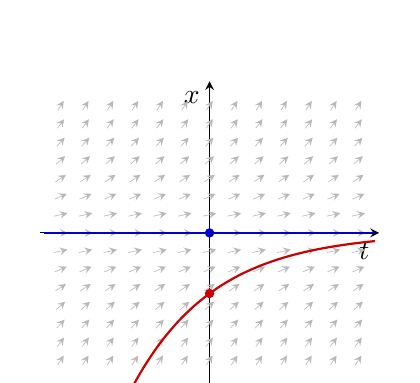
\begin{tikzpicture}[x=1.05cm,y=.77cm,>=stealth]
\clip (-2.2,-2.7) rectangle (2.2,2.7);
\draw[->] (-2.05,0)--(2.05,0) node[below left]{$t$};
\draw[->] (0,-2.5)--(0,2.5) node[below left]{$x$};
\draw[gray!55,->,line width=.23pt] (-1.8365,-2.1767)--(-1.7635,-2.0233);
\draw[gray!55,->,line width=.23pt] (-1.8413,-1.8743)--(-1.7587,-1.7257);
\draw[gray!55,->,line width=.23pt] (-1.8471,-1.5707)--(-1.7529,-1.4293);
\draw[gray!55,->,line width=.23pt] (-1.8544,-1.2653)--(-1.7456,-1.1347);
\draw[gray!55,->,line width=.23pt] (-1.8632,-0.9569)--(-1.7368,-0.8431);
\draw[gray!55,->,line width=.23pt] (-1.8729,-0.6437)--(-1.7271,-0.5563);
\draw[gray!55,->,line width=.23pt] (-1.8814,-0.3244)--(-1.7186,-0.2756);
\draw[gray!55,->,line width=.23pt] (-1.8850,0.0000)--(-1.7150,0.0000);
\draw[gray!55,->,line width=.23pt] (-1.8814,0.2756)--(-1.7186,0.3244);
\draw[gray!55,->,line width=.23pt] (-1.8729,0.5563)--(-1.7271,0.6437);
\draw[gray!55,->,line width=.23pt] (-1.8632,0.8431)--(-1.7368,0.9569);
\draw[gray!55,->,line width=.23pt] (-1.8544,1.1347)--(-1.7456,1.2653);
\draw[gray!55,->,line width=.23pt] (-1.8471,1.4293)--(-1.7529,1.5707);
\draw[gray!55,->,line width=.23pt] (-1.8413,1.7257)--(-1.7587,1.8743);
\draw[gray!55,->,line width=.23pt] (-1.8365,2.0233)--(-1.7635,2.1767);
\draw[gray!55,->,line width=.23pt] (-1.5365,-2.1767)--(-1.4635,-2.0233);
\draw[gray!55,->,line width=.23pt] (-1.5413,-1.8743)--(-1.4587,-1.7257);
\draw[gray!55,->,line width=.23pt] (-1.5471,-1.5707)--(-1.4529,-1.4293);
\draw[gray!55,->,line width=.23pt] (-1.5544,-1.2653)--(-1.4456,-1.1347);
\draw[gray!55,->,line width=.23pt] (-1.5632,-0.9569)--(-1.4368,-0.8431);
\draw[gray!55,->,line width=.23pt] (-1.5729,-0.6437)--(-1.4271,-0.5563);
\draw[gray!55,->,line width=.23pt] (-1.5814,-0.3244)--(-1.4186,-0.2756);
\draw[gray!55,->,line width=.23pt] (-1.5850,0.0000)--(-1.4150,0.0000);
\draw[gray!55,->,line width=.23pt] (-1.5814,0.2756)--(-1.4186,0.3244);
\draw[gray!55,->,line width=.23pt] (-1.5729,0.5563)--(-1.4271,0.6437);
\draw[gray!55,->,line width=.23pt] (-1.5632,0.8431)--(-1.4368,0.9569);
\draw[gray!55,->,line width=.23pt] (-1.5544,1.1347)--(-1.4456,1.2653);
\draw[gray!55,->,line width=.23pt] (-1.5471,1.4293)--(-1.4529,1.5707);
\draw[gray!55,->,line width=.23pt] (-1.5413,1.7257)--(-1.4587,1.8743);
\draw[gray!55,->,line width=.23pt] (-1.5365,2.0233)--(-1.4635,2.1767);
\draw[gray!55,->,line width=.23pt] (-1.2365,-2.1767)--(-1.1635,-2.0233);
\draw[gray!55,->,line width=.23pt] (-1.2413,-1.8743)--(-1.1587,-1.7257);
\draw[gray!55,->,line width=.23pt] (-1.2471,-1.5707)--(-1.1529,-1.4293);
\draw[gray!55,->,line width=.23pt] (-1.2544,-1.2653)--(-1.1456,-1.1347);
\draw[gray!55,->,line width=.23pt] (-1.2632,-0.9569)--(-1.1368,-0.8431);
\draw[gray!55,->,line width=.23pt] (-1.2729,-0.6437)--(-1.1271,-0.5563);
\draw[gray!55,->,line width=.23pt] (-1.2814,-0.3244)--(-1.1186,-0.2756);
\draw[gray!55,->,line width=.23pt] (-1.2850,0.0000)--(-1.1150,0.0000);
\draw[gray!55,->,line width=.23pt] (-1.2814,0.2756)--(-1.1186,0.3244);
\draw[gray!55,->,line width=.23pt] (-1.2729,0.5563)--(-1.1271,0.6437);
\draw[gray!55,->,line width=.23pt] (-1.2632,0.8431)--(-1.1368,0.9569);
\draw[gray!55,->,line width=.23pt] (-1.2544,1.1347)--(-1.1456,1.2653);
\draw[gray!55,->,line width=.23pt] (-1.2471,1.4293)--(-1.1529,1.5707);
\draw[gray!55,->,line width=.23pt] (-1.2413,1.7257)--(-1.1587,1.8743);
\draw[gray!55,->,line width=.23pt] (-1.2365,2.0233)--(-1.1635,2.1767);
\draw[gray!55,->,line width=.23pt] (-0.9365,-2.1767)--(-0.8635,-2.0233);
\draw[gray!55,->,line width=.23pt] (-0.9413,-1.8743)--(-0.8587,-1.7257);
\draw[gray!55,->,line width=.23pt] (-0.9471,-1.5707)--(-0.8529,-1.4293);
\draw[gray!55,->,line width=.23pt] (-0.9544,-1.2653)--(-0.8456,-1.1347);
\draw[gray!55,->,line width=.23pt] (-0.9632,-0.9569)--(-0.8368,-0.8431);
\draw[gray!55,->,line width=.23pt] (-0.9729,-0.6437)--(-0.8271,-0.5563);
\draw[gray!55,->,line width=.23pt] (-0.9814,-0.3244)--(-0.8186,-0.2756);
\draw[gray!55,->,line width=.23pt] (-0.9850,0.0000)--(-0.8150,0.0000);
\draw[gray!55,->,line width=.23pt] (-0.9814,0.2756)--(-0.8186,0.3244);
\draw[gray!55,->,line width=.23pt] (-0.9729,0.5563)--(-0.8271,0.6437);
\draw[gray!55,->,line width=.23pt] (-0.9632,0.8431)--(-0.8368,0.9569);
\draw[gray!55,->,line width=.23pt] (-0.9544,1.1347)--(-0.8456,1.2653);
\draw[gray!55,->,line width=.23pt] (-0.9471,1.4293)--(-0.8529,1.5707);
\draw[gray!55,->,line width=.23pt] (-0.9413,1.7257)--(-0.8587,1.8743);
\draw[gray!55,->,line width=.23pt] (-0.9365,2.0233)--(-0.8635,2.1767);
\draw[gray!55,->,line width=.23pt] (-0.6365,-2.1767)--(-0.5635,-2.0233);
\draw[gray!55,->,line width=.23pt] (-0.6413,-1.8743)--(-0.5587,-1.7257);
\draw[gray!55,->,line width=.23pt] (-0.6471,-1.5707)--(-0.5529,-1.4293);
\draw[gray!55,->,line width=.23pt] (-0.6544,-1.2653)--(-0.5456,-1.1347);
\draw[gray!55,->,line width=.23pt] (-0.6632,-0.9569)--(-0.5368,-0.8431);
\draw[gray!55,->,line width=.23pt] (-0.6729,-0.6437)--(-0.5271,-0.5563);
\draw[gray!55,->,line width=.23pt] (-0.6814,-0.3244)--(-0.5186,-0.2756);
\draw[gray!55,->,line width=.23pt] (-0.6850,0.0000)--(-0.5150,0.0000);
\draw[gray!55,->,line width=.23pt] (-0.6814,0.2756)--(-0.5186,0.3244);
\draw[gray!55,->,line width=.23pt] (-0.6729,0.5563)--(-0.5271,0.6437);
\draw[gray!55,->,line width=.23pt] (-0.6632,0.8431)--(-0.5368,0.9569);
\draw[gray!55,->,line width=.23pt] (-0.6544,1.1347)--(-0.5456,1.2653);
\draw[gray!55,->,line width=.23pt] (-0.6471,1.4293)--(-0.5529,1.5707);
\draw[gray!55,->,line width=.23pt] (-0.6413,1.7257)--(-0.5587,1.8743);
\draw[gray!55,->,line width=.23pt] (-0.6365,2.0233)--(-0.5635,2.1767);
\draw[gray!55,->,line width=.23pt] (-0.3365,-2.1767)--(-0.2635,-2.0233);
\draw[gray!55,->,line width=.23pt] (-0.3413,-1.8743)--(-0.2587,-1.7257);
\draw[gray!55,->,line width=.23pt] (-0.3471,-1.5707)--(-0.2529,-1.4293);
\draw[gray!55,->,line width=.23pt] (-0.3544,-1.2653)--(-0.2456,-1.1347);
\draw[gray!55,->,line width=.23pt] (-0.3632,-0.9569)--(-0.2368,-0.8431);
\draw[gray!55,->,line width=.23pt] (-0.3729,-0.6437)--(-0.2271,-0.5563);
\draw[gray!55,->,line width=.23pt] (-0.3814,-0.3244)--(-0.2186,-0.2756);
\draw[gray!55,->,line width=.23pt] (-0.3850,0.0000)--(-0.2150,0.0000);
\draw[gray!55,->,line width=.23pt] (-0.3814,0.2756)--(-0.2186,0.3244);
\draw[gray!55,->,line width=.23pt] (-0.3729,0.5563)--(-0.2271,0.6437);
\draw[gray!55,->,line width=.23pt] (-0.3632,0.8431)--(-0.2368,0.9569);
\draw[gray!55,->,line width=.23pt] (-0.3544,1.1347)--(-0.2456,1.2653);
\draw[gray!55,->,line width=.23pt] (-0.3471,1.4293)--(-0.2529,1.5707);
\draw[gray!55,->,line width=.23pt] (-0.3413,1.7257)--(-0.2587,1.8743);
\draw[gray!55,->,line width=.23pt] (-0.3365,2.0233)--(-0.2635,2.1767);
\draw[gray!55,->,line width=.23pt] (-0.0365,-2.1767)--(0.0365,-2.0233);
\draw[gray!55,->,line width=.23pt] (-0.0413,-1.8743)--(0.0413,-1.7257);
\draw[gray!55,->,line width=.23pt] (-0.0471,-1.5707)--(0.0471,-1.4293);
\draw[gray!55,->,line width=.23pt] (-0.0544,-1.2653)--(0.0544,-1.1347);
\draw[gray!55,->,line width=.23pt] (-0.0632,-0.9569)--(0.0632,-0.8431);
\draw[gray!55,->,line width=.23pt] (-0.0729,-0.6437)--(0.0729,-0.5563);
\draw[gray!55,->,line width=.23pt] (-0.0814,-0.3244)--(0.0814,-0.2756);
\draw[gray!55,->,line width=.23pt] (-0.0850,0.0000)--(0.0850,0.0000);
\draw[gray!55,->,line width=.23pt] (-0.0814,0.2756)--(0.0814,0.3244);
\draw[gray!55,->,line width=.23pt] (-0.0729,0.5563)--(0.0729,0.6437);
\draw[gray!55,->,line width=.23pt] (-0.0632,0.8431)--(0.0632,0.9569);
\draw[gray!55,->,line width=.23pt] (-0.0544,1.1347)--(0.0544,1.2653);
\draw[gray!55,->,line width=.23pt] (-0.0471,1.4293)--(0.0471,1.5707);
\draw[gray!55,->,line width=.23pt] (-0.0413,1.7257)--(0.0413,1.8743);
\draw[gray!55,->,line width=.23pt] (-0.0365,2.0233)--(0.0365,2.1767);
\draw[gray!55,->,line width=.23pt] (0.2635,-2.1767)--(0.3365,-2.0233);
\draw[gray!55,->,line width=.23pt] (0.2587,-1.8743)--(0.3413,-1.7257);
\draw[gray!55,->,line width=.23pt] (0.2529,-1.5707)--(0.3471,-1.4293);
\draw[gray!55,->,line width=.23pt] (0.2456,-1.2653)--(0.3544,-1.1347);
\draw[gray!55,->,line width=.23pt] (0.2368,-0.9569)--(0.3632,-0.8431);
\draw[gray!55,->,line width=.23pt] (0.2271,-0.6437)--(0.3729,-0.5563);
\draw[gray!55,->,line width=.23pt] (0.2186,-0.3244)--(0.3814,-0.2756);
\draw[gray!55,->,line width=.23pt] (0.2150,0.0000)--(0.3850,0.0000);
\draw[gray!55,->,line width=.23pt] (0.2186,0.2756)--(0.3814,0.3244);
\draw[gray!55,->,line width=.23pt] (0.2271,0.5563)--(0.3729,0.6437);
\draw[gray!55,->,line width=.23pt] (0.2368,0.8431)--(0.3632,0.9569);
\draw[gray!55,->,line width=.23pt] (0.2456,1.1347)--(0.3544,1.2653);
\draw[gray!55,->,line width=.23pt] (0.2529,1.4293)--(0.3471,1.5707);
\draw[gray!55,->,line width=.23pt] (0.2587,1.7257)--(0.3413,1.8743);
\draw[gray!55,->,line width=.23pt] (0.2635,2.0233)--(0.3365,2.1767);
\draw[gray!55,->,line width=.23pt] (0.5635,-2.1767)--(0.6365,-2.0233);
\draw[gray!55,->,line width=.23pt] (0.5587,-1.8743)--(0.6413,-1.7257);
\draw[gray!55,->,line width=.23pt] (0.5529,-1.5707)--(0.6471,-1.4293);
\draw[gray!55,->,line width=.23pt] (0.5456,-1.2653)--(0.6544,-1.1347);
\draw[gray!55,->,line width=.23pt] (0.5368,-0.9569)--(0.6632,-0.8431);
\draw[gray!55,->,line width=.23pt] (0.5271,-0.6437)--(0.6729,-0.5563);
\draw[gray!55,->,line width=.23pt] (0.5186,-0.3244)--(0.6814,-0.2756);
\draw[gray!55,->,line width=.23pt] (0.5150,0.0000)--(0.6850,0.0000);
\draw[gray!55,->,line width=.23pt] (0.5186,0.2756)--(0.6814,0.3244);
\draw[gray!55,->,line width=.23pt] (0.5271,0.5563)--(0.6729,0.6437);
\draw[gray!55,->,line width=.23pt] (0.5368,0.8431)--(0.6632,0.9569);
\draw[gray!55,->,line width=.23pt] (0.5456,1.1347)--(0.6544,1.2653);
\draw[gray!55,->,line width=.23pt] (0.5529,1.4293)--(0.6471,1.5707);
\draw[gray!55,->,line width=.23pt] (0.5587,1.7257)--(0.6413,1.8743);
\draw[gray!55,->,line width=.23pt] (0.5635,2.0233)--(0.6365,2.1767);
\draw[gray!55,->,line width=.23pt] (0.8635,-2.1767)--(0.9365,-2.0233);
\draw[gray!55,->,line width=.23pt] (0.8587,-1.8743)--(0.9413,-1.7257);
\draw[gray!55,->,line width=.23pt] (0.8529,-1.5707)--(0.9471,-1.4293);
\draw[gray!55,->,line width=.23pt] (0.8456,-1.2653)--(0.9544,-1.1347);
\draw[gray!55,->,line width=.23pt] (0.8368,-0.9569)--(0.9632,-0.8431);
\draw[gray!55,->,line width=.23pt] (0.8271,-0.6437)--(0.9729,-0.5563);
\draw[gray!55,->,line width=.23pt] (0.8186,-0.3244)--(0.9814,-0.2756);
\draw[gray!55,->,line width=.23pt] (0.8150,0.0000)--(0.9850,0.0000);
\draw[gray!55,->,line width=.23pt] (0.8186,0.2756)--(0.9814,0.3244);
\draw[gray!55,->,line width=.23pt] (0.8271,0.5563)--(0.9729,0.6437);
\draw[gray!55,->,line width=.23pt] (0.8368,0.8431)--(0.9632,0.9569);
\draw[gray!55,->,line width=.23pt] (0.8456,1.1347)--(0.9544,1.2653);
\draw[gray!55,->,line width=.23pt] (0.8529,1.4293)--(0.9471,1.5707);
\draw[gray!55,->,line width=.23pt] (0.8587,1.7257)--(0.9413,1.8743);
\draw[gray!55,->,line width=.23pt] (0.8635,2.0233)--(0.9365,2.1767);
\draw[gray!55,->,line width=.23pt] (1.1635,-2.1767)--(1.2365,-2.0233);
\draw[gray!55,->,line width=.23pt] (1.1587,-1.8743)--(1.2413,-1.7257);
\draw[gray!55,->,line width=.23pt] (1.1529,-1.5707)--(1.2471,-1.4293);
\draw[gray!55,->,line width=.23pt] (1.1456,-1.2653)--(1.2544,-1.1347);
\draw[gray!55,->,line width=.23pt] (1.1368,-0.9569)--(1.2632,-0.8431);
\draw[gray!55,->,line width=.23pt] (1.1271,-0.6437)--(1.2729,-0.5563);
\draw[gray!55,->,line width=.23pt] (1.1186,-0.3244)--(1.2814,-0.2756);
\draw[gray!55,->,line width=.23pt] (1.1150,0.0000)--(1.2850,0.0000);
\draw[gray!55,->,line width=.23pt] (1.1186,0.2756)--(1.2814,0.3244);
\draw[gray!55,->,line width=.23pt] (1.1271,0.5563)--(1.2729,0.6437);
\draw[gray!55,->,line width=.23pt] (1.1368,0.8431)--(1.2632,0.9569);
\draw[gray!55,->,line width=.23pt] (1.1456,1.1347)--(1.2544,1.2653);
\draw[gray!55,->,line width=.23pt] (1.1529,1.4293)--(1.2471,1.5707);
\draw[gray!55,->,line width=.23pt] (1.1587,1.7257)--(1.2413,1.8743);
\draw[gray!55,->,line width=.23pt] (1.1635,2.0233)--(1.2365,2.1767);
\draw[gray!55,->,line width=.23pt] (1.4635,-2.1767)--(1.5365,-2.0233);
\draw[gray!55,->,line width=.23pt] (1.4587,-1.8743)--(1.5413,-1.7257);
\draw[gray!55,->,line width=.23pt] (1.4529,-1.5707)--(1.5471,-1.4293);
\draw[gray!55,->,line width=.23pt] (1.4456,-1.2653)--(1.5544,-1.1347);
\draw[gray!55,->,line width=.23pt] (1.4368,-0.9569)--(1.5632,-0.8431);
\draw[gray!55,->,line width=.23pt] (1.4271,-0.6437)--(1.5729,-0.5563);
\draw[gray!55,->,line width=.23pt] (1.4186,-0.3244)--(1.5814,-0.2756);
\draw[gray!55,->,line width=.23pt] (1.4150,0.0000)--(1.5850,0.0000);
\draw[gray!55,->,line width=.23pt] (1.4186,0.2756)--(1.5814,0.3244);
\draw[gray!55,->,line width=.23pt] (1.4271,0.5563)--(1.5729,0.6437);
\draw[gray!55,->,line width=.23pt] (1.4368,0.8431)--(1.5632,0.9569);
\draw[gray!55,->,line width=.23pt] (1.4456,1.1347)--(1.5544,1.2653);
\draw[gray!55,->,line width=.23pt] (1.4529,1.4293)--(1.5471,1.5707);
\draw[gray!55,->,line width=.23pt] (1.4587,1.7257)--(1.5413,1.8743);
\draw[gray!55,->,line width=.23pt] (1.4635,2.0233)--(1.5365,2.1767);
\draw[gray!55,->,line width=.23pt] (1.7635,-2.1767)--(1.8365,-2.0233);
\draw[gray!55,->,line width=.23pt] (1.7587,-1.8743)--(1.8413,-1.7257);
\draw[gray!55,->,line width=.23pt] (1.7529,-1.5707)--(1.8471,-1.4293);
\draw[gray!55,->,line width=.23pt] (1.7456,-1.2653)--(1.8544,-1.1347);
\draw[gray!55,->,line width=.23pt] (1.7368,-0.9569)--(1.8632,-0.8431);
\draw[gray!55,->,line width=.23pt] (1.7271,-0.6437)--(1.8729,-0.5563);
\draw[gray!55,->,line width=.23pt] (1.7186,-0.3244)--(1.8814,-0.2756);
\draw[gray!55,->,line width=.23pt] (1.7150,0.0000)--(1.8850,0.0000);
\draw[gray!55,->,line width=.23pt] (1.7186,0.2756)--(1.8814,0.3244);
\draw[gray!55,->,line width=.23pt] (1.7271,0.5563)--(1.8729,0.6437);
\draw[gray!55,->,line width=.23pt] (1.7368,0.8431)--(1.8632,0.9569);
\draw[gray!55,->,line width=.23pt] (1.7456,1.1347)--(1.8544,1.2653);
\draw[gray!55,->,line width=.23pt] (1.7529,1.4293)--(1.8471,1.5707);
\draw[gray!55,->,line width=.23pt] (1.7587,1.7257)--(1.8413,1.8743);
\draw[gray!55,->,line width=.23pt] (1.7635,2.0233)--(1.8365,2.1767);
\draw[blue!80!black,thick] plot coordinates {(0.00000,0.00000) (-0.00000,0.00000) (-0.00001,0.00000) (-0.00011,0.00000) (-0.00111,0.00000) (-0.01111,0.00000) (-0.03611,0.00000) (-0.06111,0.00000) (-0.08611,0.00000) (-0.11111,0.00000) (-0.13611,0.00000) (-0.16111,0.00000) (-0.18611,0.00000) (-0.21111,0.00000) (-0.23611,0.00000) (-0.26111,0.00000) (-0.28611,0.00000) (-0.31111,0.00000) (-0.33611,0.00000) (-0.36111,0.00000) (-0.38611,0.00000) (-0.41111,0.00000) (-0.43611,0.00000) (-0.46111,0.00000) (-0.48611,0.00000) (-0.51111,0.00000) (-0.53611,0.00000) (-0.56111,0.00000) (-0.58611,0.00000) (-0.61111,0.00000) (-0.63611,0.00000) (-0.66111,0.00000) (-0.68611,0.00000) (-0.71111,0.00000) (-0.73611,0.00000) (-0.76111,0.00000) (-0.78611,0.00000) (-0.81111,0.00000) (-0.83611,0.00000) (-0.86111,0.00000) (-0.88611,0.00000) (-0.91111,0.00000) (-0.93611,0.00000) (-0.96111,0.00000) (-0.98611,0.00000) (-1.01111,0.00000) (-1.03611,0.00000) (-1.06111,0.00000) (-1.08611,0.00000) (-1.11111,0.00000) (-1.13611,0.00000) (-1.16111,0.00000) (-1.18611,0.00000) (-1.21111,0.00000) (-1.23611,0.00000) (-1.26111,0.00000) (-1.28611,0.00000) (-1.31111,0.00000) (-1.33611,0.00000) (-1.36111,0.00000) (-1.38611,0.00000) (-1.41111,0.00000) (-1.43611,0.00000) (-1.46111,0.00000) (-1.48611,0.00000) (-1.51111,0.00000) (-1.53611,0.00000) (-1.56111,0.00000) (-1.58611,0.00000) (-1.61111,0.00000) (-1.63611,0.00000) (-1.66111,0.00000) (-1.68611,0.00000) (-1.71111,0.00000) (-1.73611,0.00000) (-1.76111,0.00000) (-1.78611,0.00000) (-1.81111,0.00000) (-1.83611,0.00000) (-1.86111,0.00000) (-1.88611,0.00000) (-1.91111,0.00000) (-1.93611,0.00000) (-1.96111,0.00000) (-1.98611,0.00000) (-2.00000,0.00000)};
\draw[blue!80!black,thick] plot coordinates {(0.00000,0.00000) (0.00000,0.00000) (0.00001,0.00000) (0.00011,0.00000) (0.00111,0.00000) (0.01111,0.00000) (0.03611,0.00000) (0.06111,0.00000) (0.08611,0.00000) (0.11111,0.00000) (0.13611,0.00000) (0.16111,0.00000) (0.18611,0.00000) (0.21111,0.00000) (0.23611,0.00000) (0.26111,0.00000) (0.28611,0.00000) (0.31111,0.00000) (0.33611,0.00000) (0.36111,0.00000) (0.38611,0.00000) (0.41111,0.00000) (0.43611,0.00000) (0.46111,0.00000) (0.48611,0.00000) (0.51111,0.00000) (0.53611,0.00000) (0.56111,0.00000) (0.58611,0.00000) (0.61111,0.00000) (0.63611,0.00000) (0.66111,0.00000) (0.68611,0.00000) (0.71111,0.00000) (0.73611,0.00000) (0.76111,0.00000) (0.78611,0.00000) (0.81111,0.00000) (0.83611,0.00000) (0.86111,0.00000) (0.88611,0.00000) (0.91111,0.00000) (0.93611,0.00000) (0.96111,0.00000) (0.98611,0.00000) (1.01111,0.00000) (1.03611,0.00000) (1.06111,0.00000) (1.08611,0.00000) (1.11111,0.00000) (1.13611,0.00000) (1.16111,0.00000) (1.18611,0.00000) (1.21111,0.00000) (1.23611,0.00000) (1.26111,0.00000) (1.28611,0.00000) (1.31111,0.00000) (1.33611,0.00000) (1.36111,0.00000) (1.38611,0.00000) (1.41111,0.00000) (1.43611,0.00000) (1.46111,0.00000) (1.48611,0.00000) (1.51111,0.00000) (1.53611,0.00000) (1.56111,0.00000) (1.58611,0.00000) (1.61111,0.00000) (1.63611,0.00000) (1.66111,0.00000) (1.68611,0.00000) (1.71111,0.00000) (1.73611,0.00000) (1.76111,0.00000) (1.78611,0.00000) (1.81111,0.00000) (1.83611,0.00000) (1.86111,0.00000) (1.88611,0.00000) (1.91111,0.00000) (1.93611,0.00000) (1.96111,0.00000) (1.98611,0.00000) (2.00000,0.00000)};
\fill[blue!80!black] (0.00000,0.00000) circle (1.7pt);
\draw[red!80!black,thick] plot coordinates {(0.00000,-1.00000) (-0.00399,-1.00400) (-0.02899,-1.02941) (-0.05399,-1.05547) (-0.07899,-1.08219) (-0.10399,-1.10959) (-0.12899,-1.13768) (-0.15399,-1.16648) (-0.17899,-1.19601) (-0.20399,-1.22628) (-0.22899,-1.25733) (-0.25399,-1.28916) (-0.27899,-1.32179) (-0.30399,-1.35525) (-0.32899,-1.38956) (-0.35399,-1.42474) (-0.37899,-1.46081) (-0.40399,-1.49779) (-0.42899,-1.53570) (-0.45399,-1.57458) (-0.47899,-1.61444) (-0.50399,-1.65531) (-0.52899,-1.69722) (-0.55399,-1.74018) (-0.57899,-1.78423) (-0.60399,-1.82940) (-0.62899,-1.87571) (-0.65399,-1.92320) (-0.67899,-1.97188) (-0.70399,-2.02180) (-0.72899,-2.07298) (-0.75399,-2.12546) (-0.77899,-2.17927) (-0.80399,-2.23444) (-0.82899,-2.29100) (-0.85399,-2.34900) (-0.87899,-2.40846) (-0.90399,-2.46943) (-0.92899,-2.53195) (-0.95399,-2.59604) (-0.97899,-2.66176) (-1.00399,-2.72915) (-1.02899,-2.79824) (-1.05399,-2.86907) (-1.07899,-2.94170) (-1.09861,-3.00000)};
\draw[red!80!black,thick] plot coordinates {(0.00000,-1.00000) (0.00399,-0.99602) (0.02899,-0.97143) (0.05399,-0.94744) (0.07899,-0.92405) (0.10399,-0.90124) (0.12899,-0.87898) (0.15399,-0.85728) (0.17899,-0.83612) (0.20399,-0.81547) (0.22899,-0.79534) (0.25399,-0.77570) (0.27899,-0.75655) (0.30399,-0.73787) (0.32899,-0.71965) (0.35399,-0.70188) (0.37899,-0.68455) (0.40399,-0.66765) (0.42899,-0.65117) (0.45399,-0.63509) (0.47899,-0.61941) (0.50399,-0.60412) (0.52899,-0.58920) (0.55399,-0.57465) (0.57899,-0.56046) (0.60399,-0.54663) (0.62899,-0.53313) (0.65399,-0.51997) (0.67899,-0.50713) (0.70399,-0.49461) (0.72899,-0.48240) (0.75399,-0.47049) (0.77899,-0.45887) (0.80399,-0.44754) (0.82899,-0.43649) (0.85399,-0.42571) (0.87899,-0.41520) (0.90399,-0.40495) (0.92899,-0.39495) (0.95399,-0.38520) (0.97899,-0.37569) (1.00399,-0.36641) (1.02899,-0.35737) (1.05399,-0.34854) (1.07899,-0.33994) (1.10399,-0.33155) (1.12899,-0.32336) (1.15399,-0.31538) (1.17899,-0.30759) (1.20399,-0.30000) (1.22899,-0.29259) (1.25399,-0.28536) (1.27899,-0.27832) (1.30399,-0.27145) (1.32899,-0.26474) (1.35399,-0.25821) (1.37899,-0.25183) (1.40399,-0.24562) (1.42899,-0.23955) (1.45399,-0.23364) (1.47899,-0.22787) (1.50399,-0.22224) (1.52899,-0.21675) (1.55399,-0.21140) (1.57899,-0.20618) (1.60399,-0.20109) (1.62899,-0.19613) (1.65399,-0.19129) (1.67899,-0.18656) (1.70399,-0.18196) (1.72899,-0.17746) (1.75399,-0.17308) (1.77899,-0.16881) (1.80399,-0.16464) (1.82899,-0.16058) (1.85399,-0.15661) (1.87899,-0.15274) (1.90399,-0.14897) (1.92899,-0.14530) (1.95399,-0.14171) (1.97899,-0.13821) (2.00000,-0.13534)};
\fill[red!80!black] (0.00000,-1.00000) circle (1.7pt);
\end{tikzpicture}
\par\small (1)\end{minipage}\hfill\begin{minipage}[t]{.32\textwidth}\centering
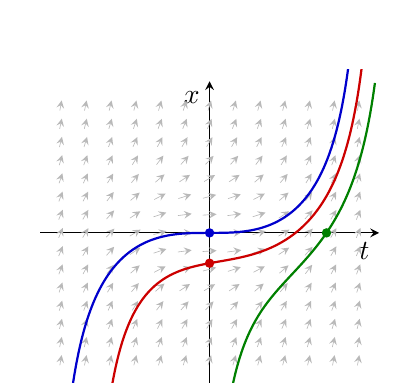
\begin{tikzpicture}[x=1.05cm,y=.77cm,>=stealth]
\clip (-2.2,-2.7) rectangle (2.2,2.7);
\draw[->] (-2.05,0)--(2.05,0) node[below left]{$t$};
\draw[->] (0,-2.5)--(0,2.5) node[below left]{$x$};
\draw[gray!55,->,line width=.23pt] (-1.8110,-2.1843)--(-1.7890,-2.0157);
\draw[gray!55,->,line width=.23pt] (-1.8130,-1.8840)--(-1.7870,-1.7160);
\draw[gray!55,->,line width=.23pt] (-1.8152,-1.5836)--(-1.7848,-1.4164);
\draw[gray!55,->,line width=.23pt] (-1.8178,-1.2831)--(-1.7822,-1.1169);
\draw[gray!55,->,line width=.23pt] (-1.8204,-0.9825)--(-1.7796,-0.8175);
\draw[gray!55,->,line width=.23pt] (-1.8227,-0.6819)--(-1.7773,-0.5181);
\draw[gray!55,->,line width=.23pt] (-1.8244,-0.3814)--(-1.7756,-0.2186);
\draw[gray!55,->,line width=.23pt] (-1.8251,-0.0812)--(-1.7749,0.0812);
\draw[gray!55,->,line width=.23pt] (-1.8244,0.2186)--(-1.7756,0.3814);
\draw[gray!55,->,line width=.23pt] (-1.8227,0.5181)--(-1.7773,0.6819);
\draw[gray!55,->,line width=.23pt] (-1.8204,0.8175)--(-1.7796,0.9825);
\draw[gray!55,->,line width=.23pt] (-1.8178,1.1169)--(-1.7822,1.2831);
\draw[gray!55,->,line width=.23pt] (-1.8152,1.4164)--(-1.7848,1.5836);
\draw[gray!55,->,line width=.23pt] (-1.8130,1.7160)--(-1.7870,1.8840);
\draw[gray!55,->,line width=.23pt] (-1.8110,2.0157)--(-1.7890,2.1843);
\draw[gray!55,->,line width=.23pt] (-1.5126,-2.1841)--(-1.4874,-2.0159);
\draw[gray!55,->,line width=.23pt] (-1.5152,-1.8836)--(-1.4848,-1.7164);
\draw[gray!55,->,line width=.23pt] (-1.5184,-1.5830)--(-1.4816,-1.4170);
\draw[gray!55,->,line width=.23pt] (-1.5222,-1.2820)--(-1.4778,-1.1180);
\draw[gray!55,->,line width=.23pt] (-1.5264,-0.9808)--(-1.4736,-0.8192);
\draw[gray!55,->,line width=.23pt] (-1.5304,-0.6794)--(-1.4696,-0.5206);
\draw[gray!55,->,line width=.23pt] (-1.5334,-0.3782)--(-1.4666,-0.2218);
\draw[gray!55,->,line width=.23pt] (-1.5345,-0.0777)--(-1.4655,0.0777);
\draw[gray!55,->,line width=.23pt] (-1.5334,0.2218)--(-1.4666,0.3782);
\draw[gray!55,->,line width=.23pt] (-1.5304,0.5206)--(-1.4696,0.6794);
\draw[gray!55,->,line width=.23pt] (-1.5264,0.8192)--(-1.4736,0.9808);
\draw[gray!55,->,line width=.23pt] (-1.5222,1.1180)--(-1.4778,1.2820);
\draw[gray!55,->,line width=.23pt] (-1.5184,1.4170)--(-1.4816,1.5830);
\draw[gray!55,->,line width=.23pt] (-1.5152,1.7164)--(-1.4848,1.8836);
\draw[gray!55,->,line width=.23pt] (-1.5126,2.0159)--(-1.4874,2.1841);
\draw[gray!55,->,line width=.23pt] (-1.2143,-2.1838)--(-1.1857,-2.0162);
\draw[gray!55,->,line width=.23pt] (-1.2178,-1.8831)--(-1.1822,-1.7169);
\draw[gray!55,->,line width=.23pt] (-1.2222,-1.5820)--(-1.1778,-1.4180);
\draw[gray!55,->,line width=.23pt] (-1.2279,-1.2803)--(-1.1721,-1.1197);
\draw[gray!55,->,line width=.23pt] (-1.2345,-0.9777)--(-1.1655,-0.8223);
\draw[gray!55,->,line width=.23pt] (-1.2413,-0.6743)--(-1.1587,-0.5257);
\draw[gray!55,->,line width=.23pt] (-1.2465,-0.3712)--(-1.1535,-0.2288);
\draw[gray!55,->,line width=.23pt] (-1.2485,-0.0698)--(-1.1515,0.0698);
\draw[gray!55,->,line width=.23pt] (-1.2465,0.2288)--(-1.1535,0.3712);
\draw[gray!55,->,line width=.23pt] (-1.2413,0.5257)--(-1.1587,0.6743);
\draw[gray!55,->,line width=.23pt] (-1.2345,0.8223)--(-1.1655,0.9777);
\draw[gray!55,->,line width=.23pt] (-1.2279,1.1197)--(-1.1721,1.2803);
\draw[gray!55,->,line width=.23pt] (-1.2222,1.4180)--(-1.1778,1.5820);
\draw[gray!55,->,line width=.23pt] (-1.2178,1.7169)--(-1.1822,1.8831);
\draw[gray!55,->,line width=.23pt] (-1.2143,2.0162)--(-1.1857,2.1838);
\draw[gray!55,->,line width=.23pt] (-0.9160,-2.1835)--(-0.8840,-2.0165);
\draw[gray!55,->,line width=.23pt] (-0.9204,-1.8825)--(-0.8796,-1.7175);
\draw[gray!55,->,line width=.23pt] (-0.9264,-1.5808)--(-0.8736,-1.4192);
\draw[gray!55,->,line width=.23pt] (-0.9345,-1.2777)--(-0.8655,-1.1223);
\draw[gray!55,->,line width=.23pt] (-0.9446,-0.9723)--(-0.8554,-0.8277);
\draw[gray!55,->,line width=.23pt] (-0.9552,-0.6646)--(-0.8448,-0.5354);
\draw[gray!55,->,line width=.23pt] (-0.9632,-0.3569)--(-0.8368,-0.2431);
\draw[gray!55,->,line width=.23pt] (-0.9661,-0.0535)--(-0.8339,0.0535);
\draw[gray!55,->,line width=.23pt] (-0.9632,0.2431)--(-0.8368,0.3569);
\draw[gray!55,->,line width=.23pt] (-0.9552,0.5354)--(-0.8448,0.6646);
\draw[gray!55,->,line width=.23pt] (-0.9446,0.8277)--(-0.8554,0.9723);
\draw[gray!55,->,line width=.23pt] (-0.9345,1.1223)--(-0.8655,1.2777);
\draw[gray!55,->,line width=.23pt] (-0.9264,1.4192)--(-0.8736,1.5808);
\draw[gray!55,->,line width=.23pt] (-0.9204,1.7175)--(-0.8796,1.8825);
\draw[gray!55,->,line width=.23pt] (-0.9160,2.0165)--(-0.8840,2.1835);
\draw[gray!55,->,line width=.23pt] (-0.6174,-2.1832)--(-0.5826,-2.0168);
\draw[gray!55,->,line width=.23pt] (-0.6227,-1.8819)--(-0.5773,-1.7181);
\draw[gray!55,->,line width=.23pt] (-0.6304,-1.5794)--(-0.5696,-1.4206);
\draw[gray!55,->,line width=.23pt] (-0.6413,-1.2743)--(-0.5587,-1.1257);
\draw[gray!55,->,line width=.23pt] (-0.6552,-0.9646)--(-0.5448,-0.8354);
\draw[gray!55,->,line width=.23pt] (-0.6690,-0.6497)--(-0.5310,-0.5503);
\draw[gray!55,->,line width=.23pt] (-0.6775,-0.3349)--(-0.5225,-0.2651);
\draw[gray!55,->,line width=.23pt] (-0.6800,-0.0288)--(-0.5200,0.0288);
\draw[gray!55,->,line width=.23pt] (-0.6775,0.2651)--(-0.5225,0.3349);
\draw[gray!55,->,line width=.23pt] (-0.6690,0.5503)--(-0.5310,0.6497);
\draw[gray!55,->,line width=.23pt] (-0.6552,0.8354)--(-0.5448,0.9646);
\draw[gray!55,->,line width=.23pt] (-0.6413,1.1257)--(-0.5587,1.2743);
\draw[gray!55,->,line width=.23pt] (-0.6304,1.4206)--(-0.5696,1.5794);
\draw[gray!55,->,line width=.23pt] (-0.6227,1.7181)--(-0.5773,1.8819);
\draw[gray!55,->,line width=.23pt] (-0.6174,2.0168)--(-0.5826,2.1832);
\draw[gray!55,->,line width=.23pt] (-0.3184,-2.1830)--(-0.2816,-2.0170);
\draw[gray!55,->,line width=.23pt] (-0.3244,-1.8814)--(-0.2756,-1.7186);
\draw[gray!55,->,line width=.23pt] (-0.3334,-1.5782)--(-0.2666,-1.4218);
\draw[gray!55,->,line width=.23pt] (-0.3465,-1.2712)--(-0.2535,-1.1288);
\draw[gray!55,->,line width=.23pt] (-0.3632,-0.9569)--(-0.2368,-0.8431);
\draw[gray!55,->,line width=.23pt] (-0.3775,-0.6349)--(-0.2225,-0.5651);
\draw[gray!55,->,line width=.23pt] (-0.3837,-0.3151)--(-0.2163,-0.2849);
\draw[gray!55,->,line width=.23pt] (-0.3847,-0.0076)--(-0.2153,0.0076);
\draw[gray!55,->,line width=.23pt] (-0.3837,0.2849)--(-0.2163,0.3151);
\draw[gray!55,->,line width=.23pt] (-0.3775,0.5651)--(-0.2225,0.6349);
\draw[gray!55,->,line width=.23pt] (-0.3632,0.8431)--(-0.2368,0.9569);
\draw[gray!55,->,line width=.23pt] (-0.3465,1.1288)--(-0.2535,1.2712);
\draw[gray!55,->,line width=.23pt] (-0.3334,1.4218)--(-0.2666,1.5782);
\draw[gray!55,->,line width=.23pt] (-0.3244,1.7186)--(-0.2756,1.8814);
\draw[gray!55,->,line width=.23pt] (-0.3184,2.0170)--(-0.2816,2.1830);
\draw[gray!55,->,line width=.23pt] (-0.0188,-2.1829)--(0.0188,-2.0171);
\draw[gray!55,->,line width=.23pt] (-0.0251,-1.8812)--(0.0251,-1.7188);
\draw[gray!55,->,line width=.23pt] (-0.0345,-1.5777)--(0.0345,-1.4223);
\draw[gray!55,->,line width=.23pt] (-0.0485,-1.2698)--(0.0485,-1.1302);
\draw[gray!55,->,line width=.23pt] (-0.0661,-0.9535)--(0.0661,-0.8465);
\draw[gray!55,->,line width=.23pt] (-0.0800,-0.6288)--(0.0800,-0.5712);
\draw[gray!55,->,line width=.23pt] (-0.0847,-0.3076)--(0.0847,-0.2924);
\draw[gray!55,->,line width=.23pt] (-0.0850,0.0000)--(0.0850,0.0000);
\draw[gray!55,->,line width=.23pt] (-0.0847,0.2924)--(0.0847,0.3076);
\draw[gray!55,->,line width=.23pt] (-0.0800,0.5712)--(0.0800,0.6288);
\draw[gray!55,->,line width=.23pt] (-0.0661,0.8465)--(0.0661,0.9535);
\draw[gray!55,->,line width=.23pt] (-0.0485,1.1302)--(0.0485,1.2698);
\draw[gray!55,->,line width=.23pt] (-0.0345,1.4223)--(0.0345,1.5777);
\draw[gray!55,->,line width=.23pt] (-0.0251,1.7188)--(0.0251,1.8812);
\draw[gray!55,->,line width=.23pt] (-0.0188,2.0171)--(0.0188,2.1829);
\draw[gray!55,->,line width=.23pt] (0.2816,-2.1830)--(0.3184,-2.0170);
\draw[gray!55,->,line width=.23pt] (0.2756,-1.8814)--(0.3244,-1.7186);
\draw[gray!55,->,line width=.23pt] (0.2666,-1.5782)--(0.3334,-1.4218);
\draw[gray!55,->,line width=.23pt] (0.2535,-1.2712)--(0.3465,-1.1288);
\draw[gray!55,->,line width=.23pt] (0.2368,-0.9569)--(0.3632,-0.8431);
\draw[gray!55,->,line width=.23pt] (0.2225,-0.6349)--(0.3775,-0.5651);
\draw[gray!55,->,line width=.23pt] (0.2163,-0.3151)--(0.3837,-0.2849);
\draw[gray!55,->,line width=.23pt] (0.2153,-0.0076)--(0.3847,0.0076);
\draw[gray!55,->,line width=.23pt] (0.2163,0.2849)--(0.3837,0.3151);
\draw[gray!55,->,line width=.23pt] (0.2225,0.5651)--(0.3775,0.6349);
\draw[gray!55,->,line width=.23pt] (0.2368,0.8431)--(0.3632,0.9569);
\draw[gray!55,->,line width=.23pt] (0.2535,1.1288)--(0.3465,1.2712);
\draw[gray!55,->,line width=.23pt] (0.2666,1.4218)--(0.3334,1.5782);
\draw[gray!55,->,line width=.23pt] (0.2756,1.7186)--(0.3244,1.8814);
\draw[gray!55,->,line width=.23pt] (0.2816,2.0170)--(0.3184,2.1830);
\draw[gray!55,->,line width=.23pt] (0.5826,-2.1832)--(0.6174,-2.0168);
\draw[gray!55,->,line width=.23pt] (0.5773,-1.8819)--(0.6227,-1.7181);
\draw[gray!55,->,line width=.23pt] (0.5696,-1.5794)--(0.6304,-1.4206);
\draw[gray!55,->,line width=.23pt] (0.5587,-1.2743)--(0.6413,-1.1257);
\draw[gray!55,->,line width=.23pt] (0.5448,-0.9646)--(0.6552,-0.8354);
\draw[gray!55,->,line width=.23pt] (0.5310,-0.6497)--(0.6690,-0.5503);
\draw[gray!55,->,line width=.23pt] (0.5225,-0.3349)--(0.6775,-0.2651);
\draw[gray!55,->,line width=.23pt] (0.5200,-0.0288)--(0.6800,0.0288);
\draw[gray!55,->,line width=.23pt] (0.5225,0.2651)--(0.6775,0.3349);
\draw[gray!55,->,line width=.23pt] (0.5310,0.5503)--(0.6690,0.6497);
\draw[gray!55,->,line width=.23pt] (0.5448,0.8354)--(0.6552,0.9646);
\draw[gray!55,->,line width=.23pt] (0.5587,1.1257)--(0.6413,1.2743);
\draw[gray!55,->,line width=.23pt] (0.5696,1.4206)--(0.6304,1.5794);
\draw[gray!55,->,line width=.23pt] (0.5773,1.7181)--(0.6227,1.8819);
\draw[gray!55,->,line width=.23pt] (0.5826,2.0168)--(0.6174,2.1832);
\draw[gray!55,->,line width=.23pt] (0.8840,-2.1835)--(0.9160,-2.0165);
\draw[gray!55,->,line width=.23pt] (0.8796,-1.8825)--(0.9204,-1.7175);
\draw[gray!55,->,line width=.23pt] (0.8736,-1.5808)--(0.9264,-1.4192);
\draw[gray!55,->,line width=.23pt] (0.8655,-1.2777)--(0.9345,-1.1223);
\draw[gray!55,->,line width=.23pt] (0.8554,-0.9723)--(0.9446,-0.8277);
\draw[gray!55,->,line width=.23pt] (0.8448,-0.6646)--(0.9552,-0.5354);
\draw[gray!55,->,line width=.23pt] (0.8368,-0.3569)--(0.9632,-0.2431);
\draw[gray!55,->,line width=.23pt] (0.8339,-0.0535)--(0.9661,0.0535);
\draw[gray!55,->,line width=.23pt] (0.8368,0.2431)--(0.9632,0.3569);
\draw[gray!55,->,line width=.23pt] (0.8448,0.5354)--(0.9552,0.6646);
\draw[gray!55,->,line width=.23pt] (0.8554,0.8277)--(0.9446,0.9723);
\draw[gray!55,->,line width=.23pt] (0.8655,1.1223)--(0.9345,1.2777);
\draw[gray!55,->,line width=.23pt] (0.8736,1.4192)--(0.9264,1.5808);
\draw[gray!55,->,line width=.23pt] (0.8796,1.7175)--(0.9204,1.8825);
\draw[gray!55,->,line width=.23pt] (0.8840,2.0165)--(0.9160,2.1835);
\draw[gray!55,->,line width=.23pt] (1.1857,-2.1838)--(1.2143,-2.0162);
\draw[gray!55,->,line width=.23pt] (1.1822,-1.8831)--(1.2178,-1.7169);
\draw[gray!55,->,line width=.23pt] (1.1778,-1.5820)--(1.2222,-1.4180);
\draw[gray!55,->,line width=.23pt] (1.1721,-1.2803)--(1.2279,-1.1197);
\draw[gray!55,->,line width=.23pt] (1.1655,-0.9777)--(1.2345,-0.8223);
\draw[gray!55,->,line width=.23pt] (1.1587,-0.6743)--(1.2413,-0.5257);
\draw[gray!55,->,line width=.23pt] (1.1535,-0.3712)--(1.2465,-0.2288);
\draw[gray!55,->,line width=.23pt] (1.1515,-0.0698)--(1.2485,0.0698);
\draw[gray!55,->,line width=.23pt] (1.1535,0.2288)--(1.2465,0.3712);
\draw[gray!55,->,line width=.23pt] (1.1587,0.5257)--(1.2413,0.6743);
\draw[gray!55,->,line width=.23pt] (1.1655,0.8223)--(1.2345,0.9777);
\draw[gray!55,->,line width=.23pt] (1.1721,1.1197)--(1.2279,1.2803);
\draw[gray!55,->,line width=.23pt] (1.1778,1.4180)--(1.2222,1.5820);
\draw[gray!55,->,line width=.23pt] (1.1822,1.7169)--(1.2178,1.8831);
\draw[gray!55,->,line width=.23pt] (1.1857,2.0162)--(1.2143,2.1838);
\draw[gray!55,->,line width=.23pt] (1.4874,-2.1841)--(1.5126,-2.0159);
\draw[gray!55,->,line width=.23pt] (1.4848,-1.8836)--(1.5152,-1.7164);
\draw[gray!55,->,line width=.23pt] (1.4816,-1.5830)--(1.5184,-1.4170);
\draw[gray!55,->,line width=.23pt] (1.4778,-1.2820)--(1.5222,-1.1180);
\draw[gray!55,->,line width=.23pt] (1.4736,-0.9808)--(1.5264,-0.8192);
\draw[gray!55,->,line width=.23pt] (1.4696,-0.6794)--(1.5304,-0.5206);
\draw[gray!55,->,line width=.23pt] (1.4666,-0.3782)--(1.5334,-0.2218);
\draw[gray!55,->,line width=.23pt] (1.4655,-0.0777)--(1.5345,0.0777);
\draw[gray!55,->,line width=.23pt] (1.4666,0.2218)--(1.5334,0.3782);
\draw[gray!55,->,line width=.23pt] (1.4696,0.5206)--(1.5304,0.6794);
\draw[gray!55,->,line width=.23pt] (1.4736,0.8192)--(1.5264,0.9808);
\draw[gray!55,->,line width=.23pt] (1.4778,1.1180)--(1.5222,1.2820);
\draw[gray!55,->,line width=.23pt] (1.4816,1.4170)--(1.5184,1.5830);
\draw[gray!55,->,line width=.23pt] (1.4848,1.7164)--(1.5152,1.8836);
\draw[gray!55,->,line width=.23pt] (1.4874,2.0159)--(1.5126,2.1841);
\draw[gray!55,->,line width=.23pt] (1.7890,-2.1843)--(1.8110,-2.0157);
\draw[gray!55,->,line width=.23pt] (1.7870,-1.8840)--(1.8130,-1.7160);
\draw[gray!55,->,line width=.23pt] (1.7848,-1.5836)--(1.8152,-1.4164);
\draw[gray!55,->,line width=.23pt] (1.7822,-1.2831)--(1.8178,-1.1169);
\draw[gray!55,->,line width=.23pt] (1.7796,-0.9825)--(1.8204,-0.8175);
\draw[gray!55,->,line width=.23pt] (1.7773,-0.6819)--(1.8227,-0.5181);
\draw[gray!55,->,line width=.23pt] (1.7756,-0.3814)--(1.8244,-0.2186);
\draw[gray!55,->,line width=.23pt] (1.7749,-0.0812)--(1.8251,0.0812);
\draw[gray!55,->,line width=.23pt] (1.7756,0.2186)--(1.8244,0.3814);
\draw[gray!55,->,line width=.23pt] (1.7773,0.5181)--(1.8227,0.6819);
\draw[gray!55,->,line width=.23pt] (1.7796,0.8175)--(1.8204,0.9825);
\draw[gray!55,->,line width=.23pt] (1.7822,1.1169)--(1.8178,1.2831);
\draw[gray!55,->,line width=.23pt] (1.7848,1.4164)--(1.8152,1.5836);
\draw[gray!55,->,line width=.23pt] (1.7870,1.7160)--(1.8130,1.8840);
\draw[gray!55,->,line width=.23pt] (1.7890,2.0157)--(1.8110,2.1843);
\draw[blue!80!black,thick] plot coordinates {(0.00000,0.00000) (-0.00010,-0.00000) (-0.00110,-0.00000) (-0.01110,-0.00000) (-0.03610,-0.00002) (-0.06110,-0.00008) (-0.08610,-0.00021) (-0.11110,-0.00046) (-0.13610,-0.00084) (-0.16110,-0.00139) (-0.18610,-0.00215) (-0.21110,-0.00314) (-0.23610,-0.00439) (-0.26110,-0.00593) (-0.28610,-0.00781) (-0.31110,-0.01004) (-0.33610,-0.01266) (-0.36110,-0.01571) (-0.38610,-0.01921) (-0.41110,-0.02319) (-0.43610,-0.02769) (-0.46110,-0.03275) (-0.48610,-0.03839) (-0.51110,-0.04465) (-0.53610,-0.05156) (-0.56110,-0.05916) (-0.58610,-0.06749) (-0.61110,-0.07658) (-0.63610,-0.08647) (-0.66110,-0.09720) (-0.68610,-0.10881) (-0.71110,-0.12134) (-0.73610,-0.13484) (-0.76110,-0.14936) (-0.78610,-0.16494) (-0.81110,-0.18163) (-0.83610,-0.19950) (-0.86110,-0.21860) (-0.88610,-0.23899) (-0.91110,-0.26074) (-0.93610,-0.28392) (-0.96110,-0.30861) (-0.98610,-0.33489) (-1.01110,-0.36287) (-1.03610,-0.39263) (-1.06110,-0.42429) (-1.08610,-0.45797) (-1.11110,-0.49380) (-1.13610,-0.53194) (-1.16110,-0.57254) (-1.18610,-0.61580) (-1.21110,-0.66192) (-1.23610,-0.71113) (-1.26110,-0.76370) (-1.28610,-0.81992) (-1.31110,-0.88013) (-1.33610,-0.94474) (-1.36110,-1.01418) (-1.38399,-1.08244) (-1.40481,-1.14885) (-1.42412,-1.21441) (-1.44219,-1.27965) (-1.45925,-1.34489) (-1.47542,-1.41038) (-1.49081,-1.47629) (-1.50550,-1.54275) (-1.51957,-1.60987) (-1.53306,-1.67774) (-1.54602,-1.74644) (-1.55849,-1.81605) (-1.57050,-1.88662) (-1.58209,-1.95823) (-1.59327,-2.03091) (-1.60408,-2.10474) (-1.61453,-2.17975) (-1.62464,-2.25601) (-1.63443,-2.33355) (-1.64392,-2.41243) (-1.65311,-2.49269) (-1.66202,-2.57439) (-1.67067,-2.65757) (-1.67906,-2.74228) (-1.68721,-2.82856) (-1.69512,-2.91648) (-1.70230,-3.00000)};
\draw[blue!80!black,thick] plot coordinates {(0.00000,0.00000) (0.00010,0.00000) (0.00110,0.00000) (0.01110,0.00000) (0.03610,0.00002) (0.06110,0.00008) (0.08610,0.00021) (0.11110,0.00046) (0.13610,0.00084) (0.16110,0.00139) (0.18610,0.00215) (0.21110,0.00314) (0.23610,0.00439) (0.26110,0.00593) (0.28610,0.00781) (0.31110,0.01004) (0.33610,0.01266) (0.36110,0.01571) (0.38610,0.01921) (0.41110,0.02319) (0.43610,0.02769) (0.46110,0.03275) (0.48610,0.03839) (0.51110,0.04465) (0.53610,0.05156) (0.56110,0.05916) (0.58610,0.06749) (0.61110,0.07658) (0.63610,0.08647) (0.66110,0.09720) (0.68610,0.10881) (0.71110,0.12134) (0.73610,0.13484) (0.76110,0.14936) (0.78610,0.16494) (0.81110,0.18163) (0.83610,0.19950) (0.86110,0.21860) (0.88610,0.23899) (0.91110,0.26074) (0.93610,0.28392) (0.96110,0.30861) (0.98610,0.33489) (1.01110,0.36287) (1.03610,0.39263) (1.06110,0.42429) (1.08610,0.45797) (1.11110,0.49380) (1.13610,0.53194) (1.16110,0.57254) (1.18610,0.61580) (1.21110,0.66192) (1.23610,0.71113) (1.26110,0.76370) (1.28610,0.81992) (1.31110,0.88013) (1.33610,0.94474) (1.36110,1.01418) (1.38399,1.08244) (1.40481,1.14885) (1.42412,1.21441) (1.44219,1.27965) (1.45925,1.34489) (1.47542,1.41038) (1.49081,1.47629) (1.50550,1.54275) (1.51957,1.60987) (1.53306,1.67774) (1.54602,1.74644) (1.55849,1.81605) (1.57050,1.88662) (1.58209,1.95823) (1.59327,2.03091) (1.60408,2.10474) (1.61453,2.17975) (1.62464,2.25601) (1.63443,2.33355) (1.64392,2.41243) (1.65311,2.49269) (1.66202,2.57439) (1.67067,2.65757) (1.67906,2.74228) (1.68721,2.82856) (1.69512,2.91648) (1.70230,3.00000)};
\fill[blue!80!black] (0.00000,0.00000) circle (1.7pt);
\draw[red!80!black,thick] plot coordinates {(0.00000,-0.50000) (-0.00452,-0.50113) (-0.02952,-0.50750) (-0.05452,-0.51407) (-0.07952,-0.52087) (-0.10452,-0.52796) (-0.12952,-0.53537) (-0.15452,-0.54315) (-0.17952,-0.55133) (-0.20452,-0.55997) (-0.22952,-0.56912) (-0.25452,-0.57882) (-0.27952,-0.58912) (-0.30452,-0.60010) (-0.32952,-0.61179) (-0.35452,-0.62426) (-0.37952,-0.63758) (-0.40452,-0.65181) (-0.42952,-0.66703) (-0.45452,-0.68331) (-0.47952,-0.70073) (-0.50452,-0.71938) (-0.52952,-0.73936) (-0.55452,-0.76077) (-0.57952,-0.78372) (-0.60452,-0.80832) (-0.62949,-0.83467) (-0.65381,-0.86219) (-0.67749,-0.89087) (-0.70051,-0.92068) (-0.72290,-0.95165) (-0.74467,-0.98374) (-0.76582,-1.01697) (-0.78637,-1.05132) (-0.80634,-1.08680) (-0.82573,-1.12339) (-0.84456,-1.16109) (-0.86285,-1.19990) (-0.88062,-1.23983) (-0.89787,-1.28087) (-0.91462,-1.32302) (-0.93090,-1.36630) (-0.94670,-1.41070) (-0.96206,-1.45623) (-0.97698,-1.50291) (-0.99147,-1.55074) (-1.00556,-1.59974) (-1.01925,-1.64991) (-1.03256,-1.70127) (-1.04550,-1.75385) (-1.05808,-1.80765) (-1.07031,-1.86269) (-1.08221,-1.91899) (-1.09378,-1.97658) (-1.10504,-2.03548) (-1.11599,-2.09571) (-1.12664,-2.15729) (-1.13702,-2.22025) (-1.14711,-2.28462) (-1.15694,-2.35043) (-1.16650,-2.41770) (-1.17582,-2.48647) (-1.18488,-2.55676) (-1.19372,-2.62862) (-1.20232,-2.70207) (-1.21070,-2.77715) (-1.21886,-2.85389) (-1.22682,-2.93234) (-1.23338,-3.00000)};
\draw[red!80!black,thick] plot coordinates {(0.00000,-0.50000) (0.00459,-0.49885) (0.02959,-0.49270) (0.05459,-0.48666) (0.07959,-0.48070) (0.10459,-0.47478) (0.12959,-0.46887) (0.15459,-0.46294) (0.17959,-0.45695) (0.20459,-0.45087) (0.22959,-0.44468) (0.25459,-0.43834) (0.27959,-0.43182) (0.30459,-0.42510) (0.32959,-0.41814) (0.35459,-0.41092) (0.37959,-0.40340) (0.40459,-0.39557) (0.42959,-0.38738) (0.45459,-0.37883) (0.47959,-0.36987) (0.50459,-0.36048) (0.52959,-0.35063) (0.55459,-0.34030) (0.57959,-0.32945) (0.60459,-0.31806) (0.62959,-0.30611) (0.65459,-0.29355) (0.67959,-0.28036) (0.70459,-0.26652) (0.72959,-0.25198) (0.75459,-0.23672) (0.77959,-0.22070) (0.80459,-0.20388) (0.82959,-0.18624) (0.85459,-0.16772) (0.87959,-0.14830) (0.90459,-0.12792) (0.92959,-0.10655) (0.95459,-0.08413) (0.97959,-0.06062) (1.00459,-0.03595) (1.02959,-0.01007) (1.04873,0.01059) (1.06708,0.03114) (1.08727,0.05460) (1.10855,0.08036) (1.13044,0.10799) (1.15265,0.13726) (1.17498,0.16804) (1.19734,0.20026) (1.21966,0.23390) (1.24188,0.26897) (1.26399,0.30550) (1.28596,0.34354) (1.30781,0.38317) (1.32953,0.42448) (1.35114,0.46761) (1.37266,0.51270) (1.39413,0.55995) (1.41558,0.60963) (1.43709,0.66207) (1.45874,0.71777) (1.48069,0.77744) (1.50319,0.84229) (1.52680,0.91469) (1.55180,0.99675) (1.57680,1.08500) (1.59687,1.16083) (1.61694,1.24160) (1.63541,1.32077) (1.65241,1.39814) (1.66828,1.47461) (1.68321,1.55070) (1.69735,1.62677) (1.71079,1.70306) (1.72362,1.77978) (1.73590,1.85708) (1.74766,1.93509) (1.75897,2.01391) (1.76985,2.09365) (1.78033,2.17438) (1.79044,2.25620) (1.80019,2.33916) (1.80962,2.42335) (1.81874,2.50882) (1.82757,2.59564) (1.83612,2.68388) (1.84440,2.77358) (1.85243,2.86481) (1.86022,2.95763) (1.86365,3.00000)};
\fill[red!80!black] (0.00000,-0.50000) circle (1.7pt);
\draw[green!50!black,thick] plot coordinates {(1.41421,0.00000) (1.41411,-0.00020) (1.41311,-0.00220) (1.40311,-0.02203) (1.38794,-0.05160) (1.37023,-0.08537) (1.35006,-0.12291) (1.32727,-0.16421) (1.30227,-0.20830) (1.27727,-0.25122) (1.25227,-0.29306) (1.22727,-0.33395) (1.20227,-0.37398) (1.17727,-0.41325) (1.15227,-0.45185) (1.12727,-0.48988) (1.10227,-0.52742) (1.07727,-0.56457) (1.05227,-0.60141) (1.02727,-0.63805) (1.00227,-0.67456) (0.97727,-0.71106) (0.95227,-0.74763) (0.92727,-0.78438) (0.90227,-0.82142) (0.87727,-0.85886) (0.85227,-0.89683) (0.82727,-0.93544) (0.80227,-0.97485) (0.77727,-1.01519) (0.75306,-1.05532) (0.72992,-1.09479) (0.70774,-1.13379) (0.68643,-1.17247) (0.66591,-1.21099) (0.64612,-1.24946) (0.62700,-1.28799) (0.60849,-1.32667) (0.59057,-1.36559) (0.57319,-1.40481) (0.55633,-1.44440) (0.53996,-1.48442) (0.52405,-1.52494) (0.50859,-1.56600) (0.49354,-1.60765) (0.47891,-1.64995) (0.46465,-1.69293) (0.45077,-1.73664) (0.43726,-1.78113) (0.42408,-1.82643) (0.41124,-1.87258) (0.39873,-1.91962) (0.38652,-1.96760) (0.37462,-2.01654) (0.36301,-2.06649) (0.35169,-2.11749) (0.34064,-2.16956) (0.32987,-2.22275) (0.31935,-2.27709) (0.30909,-2.33262) (0.29907,-2.38938) (0.28929,-2.44740) (0.27975,-2.50673) (0.27043,-2.56739) (0.26134,-2.62943) (0.25246,-2.69289) (0.24379,-2.75780) (0.23532,-2.82420) (0.22706,-2.89214) (0.21899,-2.96165) (0.21470,-3.00000)};
\draw[green!50!black,thick] plot coordinates {(1.41421,0.00000) (1.41431,0.00020) (1.41531,0.00220) (1.42531,0.02238) (1.44073,0.05407) (1.45804,0.09051) (1.47625,0.12995) (1.49494,0.17160) (1.51384,0.21509) (1.53281,0.26020) (1.55179,0.30686) (1.57072,0.35507) (1.58957,0.40487) (1.60834,0.45635) (1.62704,0.50963) (1.64566,0.56489) (1.66425,0.62236) (1.68284,0.68231) (1.70147,0.74514) (1.72022,0.81140) (1.73922,0.88188) (1.75869,0.95788) (1.77904,1.04192) (1.80156,1.14090) (1.82138,1.23387) (1.84120,1.33298) (1.85733,1.41864) (1.87345,1.50931) (1.88843,1.59848) (1.90240,1.68630) (1.91553,1.77343) (1.92795,1.86034) (1.93977,1.94735) (1.95104,2.03469) (1.96183,2.12258) (1.97217,2.21116) (1.98211,2.30057) (1.99167,2.39093) (2.00000,2.47334)};
\fill[green!50!black] (1.41421,0.00000) circle (1.7pt);
\end{tikzpicture}
\par\small (2)\end{minipage}\hfill\begin{minipage}[t]{.32\textwidth}\centering
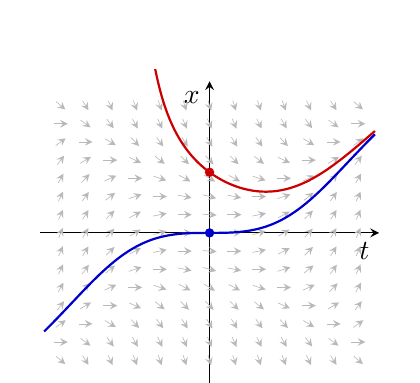
\begin{tikzpicture}[x=1.05cm,y=.77cm,>=stealth]
\clip (-2.2,-2.7) rectangle (2.2,2.7);
\draw[->] (-2.05,0)--(2.05,0) node[below left]{$t$};
\draw[->] (0,-2.5)--(0,2.5) node[below left]{$x$};
\draw[gray!55,->,line width=.23pt] (-1.8552,-2.0354)--(-1.7448,-2.1646);
\draw[gray!55,->,line width=.23pt] (-1.8850,-1.8000)--(-1.7150,-1.8000);
\draw[gray!55,->,line width=.23pt] (-1.8604,-1.5598)--(-1.7396,-1.4402);
\draw[gray!55,->,line width=.23pt] (-1.8413,-1.2743)--(-1.7587,-1.1257);
\draw[gray!55,->,line width=.23pt] (-1.8323,-0.9786)--(-1.7677,-0.8214);
\draw[gray!55,->,line width=.23pt] (-1.8279,-0.6803)--(-1.7721,-0.5197);
\draw[gray!55,->,line width=.23pt] (-1.8257,-0.3810)--(-1.7743,-0.2190);
\draw[gray!55,->,line width=.23pt] (-1.8251,-0.0812)--(-1.7749,0.0812);
\draw[gray!55,->,line width=.23pt] (-1.8257,0.2190)--(-1.7743,0.3810);
\draw[gray!55,->,line width=.23pt] (-1.8279,0.5197)--(-1.7721,0.6803);
\draw[gray!55,->,line width=.23pt] (-1.8323,0.8214)--(-1.7677,0.9786);
\draw[gray!55,->,line width=.23pt] (-1.8413,1.1257)--(-1.7587,1.2743);
\draw[gray!55,->,line width=.23pt] (-1.8604,1.4402)--(-1.7396,1.5598);
\draw[gray!55,->,line width=.23pt] (-1.8850,1.8000)--(-1.7150,1.8000);
\draw[gray!55,->,line width=.23pt] (-1.8552,2.1646)--(-1.7448,2.0354);
\draw[gray!55,->,line width=.23pt] (-1.5357,-2.0229)--(-1.4643,-2.1771);
\draw[gray!55,->,line width=.23pt] (-1.5604,-1.7402)--(-1.4396,-1.8598);
\draw[gray!55,->,line width=.23pt] (-1.5850,-1.5000)--(-1.4150,-1.5000);
\draw[gray!55,->,line width=.23pt] (-1.5661,-1.2535)--(-1.4339,-1.1465);
\draw[gray!55,->,line width=.23pt] (-1.5485,-0.9698)--(-1.4515,-0.8302);
\draw[gray!55,->,line width=.23pt] (-1.5398,-0.6751)--(-1.4602,-0.5249);
\draw[gray!55,->,line width=.23pt] (-1.5357,-0.3771)--(-1.4643,-0.2229);
\draw[gray!55,->,line width=.23pt] (-1.5345,-0.0777)--(-1.4655,0.0777);
\draw[gray!55,->,line width=.23pt] (-1.5357,0.2229)--(-1.4643,0.3771);
\draw[gray!55,->,line width=.23pt] (-1.5398,0.5249)--(-1.4602,0.6751);
\draw[gray!55,->,line width=.23pt] (-1.5485,0.8302)--(-1.4515,0.9698);
\draw[gray!55,->,line width=.23pt] (-1.5661,1.1465)--(-1.4339,1.2535);
\draw[gray!55,->,line width=.23pt] (-1.5850,1.5000)--(-1.4150,1.5000);
\draw[gray!55,->,line width=.23pt] (-1.5604,1.8598)--(-1.4396,1.7402);
\draw[gray!55,->,line width=.23pt] (-1.5357,2.1771)--(-1.4643,2.0229);
\draw[gray!55,->,line width=.23pt] (-1.2271,-2.0194)--(-1.1729,-2.1806);
\draw[gray!55,->,line width=.23pt] (-1.2413,-1.7257)--(-1.1587,-1.8743);
\draw[gray!55,->,line width=.23pt] (-1.2661,-1.4465)--(-1.1339,-1.5535);
\draw[gray!55,->,line width=.23pt] (-1.2850,-1.2000)--(-1.1150,-1.2000);
\draw[gray!55,->,line width=.23pt] (-1.2719,-0.9453)--(-1.1281,-0.8547);
\draw[gray!55,->,line width=.23pt] (-1.2577,-0.6624)--(-1.1423,-0.5376);
\draw[gray!55,->,line width=.23pt] (-1.2506,-0.3683)--(-1.1494,-0.2317);
\draw[gray!55,->,line width=.23pt] (-1.2485,-0.0698)--(-1.1515,0.0698);
\draw[gray!55,->,line width=.23pt] (-1.2506,0.2317)--(-1.1494,0.3683);
\draw[gray!55,->,line width=.23pt] (-1.2577,0.5376)--(-1.1423,0.6624);
\draw[gray!55,->,line width=.23pt] (-1.2719,0.8547)--(-1.1281,0.9453);
\draw[gray!55,->,line width=.23pt] (-1.2850,1.2000)--(-1.1150,1.2000);
\draw[gray!55,->,line width=.23pt] (-1.2661,1.5535)--(-1.1339,1.4465);
\draw[gray!55,->,line width=.23pt] (-1.2413,1.8743)--(-1.1587,1.7257);
\draw[gray!55,->,line width=.23pt] (-1.2271,2.1806)--(-1.1729,2.0194);
\draw[gray!55,->,line width=.23pt] (-0.9227,-2.0181)--(-0.8773,-2.1819);
\draw[gray!55,->,line width=.23pt] (-0.9323,-1.7214)--(-0.8677,-1.8786);
\draw[gray!55,->,line width=.23pt] (-0.9485,-1.4302)--(-0.8515,-1.5698);
\draw[gray!55,->,line width=.23pt] (-0.9719,-1.1547)--(-0.8281,-1.2453);
\draw[gray!55,->,line width=.23pt] (-0.9850,-0.9000)--(-0.8150,-0.9000);
\draw[gray!55,->,line width=.23pt] (-0.9775,-0.6349)--(-0.8225,-0.5651);
\draw[gray!55,->,line width=.23pt] (-0.9690,-0.3497)--(-0.8310,-0.2503);
\draw[gray!55,->,line width=.23pt] (-0.9661,-0.0535)--(-0.8339,0.0535);
\draw[gray!55,->,line width=.23pt] (-0.9690,0.2503)--(-0.8310,0.3497);
\draw[gray!55,->,line width=.23pt] (-0.9775,0.5651)--(-0.8225,0.6349);
\draw[gray!55,->,line width=.23pt] (-0.9850,0.9000)--(-0.8150,0.9000);
\draw[gray!55,->,line width=.23pt] (-0.9719,1.2453)--(-0.8281,1.1547);
\draw[gray!55,->,line width=.23pt] (-0.9485,1.5698)--(-0.8515,1.4302);
\draw[gray!55,->,line width=.23pt] (-0.9323,1.8786)--(-0.8677,1.7214);
\draw[gray!55,->,line width=.23pt] (-0.9227,2.1819)--(-0.8773,2.0181);
\draw[gray!55,->,line width=.23pt] (-0.6204,-2.0175)--(-0.5796,-2.1825);
\draw[gray!55,->,line width=.23pt] (-0.6279,-1.7197)--(-0.5721,-1.8803);
\draw[gray!55,->,line width=.23pt] (-0.6398,-1.4249)--(-0.5602,-1.5751);
\draw[gray!55,->,line width=.23pt] (-0.6577,-1.1376)--(-0.5423,-1.2624);
\draw[gray!55,->,line width=.23pt] (-0.6775,-0.8651)--(-0.5225,-0.9349);
\draw[gray!55,->,line width=.23pt] (-0.6850,-0.6000)--(-0.5150,-0.6000);
\draw[gray!55,->,line width=.23pt] (-0.6821,-0.3222)--(-0.5179,-0.2778);
\draw[gray!55,->,line width=.23pt] (-0.6800,-0.0288)--(-0.5200,0.0288);
\draw[gray!55,->,line width=.23pt] (-0.6821,0.2778)--(-0.5179,0.3222);
\draw[gray!55,->,line width=.23pt] (-0.6850,0.6000)--(-0.5150,0.6000);
\draw[gray!55,->,line width=.23pt] (-0.6775,0.9349)--(-0.5225,0.8651);
\draw[gray!55,->,line width=.23pt] (-0.6577,1.2624)--(-0.5423,1.1376);
\draw[gray!55,->,line width=.23pt] (-0.6398,1.5751)--(-0.5602,1.4249);
\draw[gray!55,->,line width=.23pt] (-0.6279,1.8803)--(-0.5721,1.7197);
\draw[gray!55,->,line width=.23pt] (-0.6204,2.1825)--(-0.5796,2.0175);
\draw[gray!55,->,line width=.23pt] (-0.3192,-2.0172)--(-0.2808,-2.1828);
\draw[gray!55,->,line width=.23pt] (-0.3257,-1.7190)--(-0.2743,-1.8810);
\draw[gray!55,->,line width=.23pt] (-0.3357,-1.4229)--(-0.2643,-1.5771);
\draw[gray!55,->,line width=.23pt] (-0.3506,-1.1317)--(-0.2494,-1.2683);
\draw[gray!55,->,line width=.23pt] (-0.3690,-0.8503)--(-0.2310,-0.9497);
\draw[gray!55,->,line width=.23pt] (-0.3821,-0.5778)--(-0.2179,-0.6222);
\draw[gray!55,->,line width=.23pt] (-0.3850,-0.3000)--(-0.2150,-0.3000);
\draw[gray!55,->,line width=.23pt] (-0.3847,-0.0076)--(-0.2153,0.0076);
\draw[gray!55,->,line width=.23pt] (-0.3850,0.3000)--(-0.2150,0.3000);
\draw[gray!55,->,line width=.23pt] (-0.3821,0.6222)--(-0.2179,0.5778);
\draw[gray!55,->,line width=.23pt] (-0.3690,0.9497)--(-0.2310,0.8503);
\draw[gray!55,->,line width=.23pt] (-0.3506,1.2683)--(-0.2494,1.1317);
\draw[gray!55,->,line width=.23pt] (-0.3357,1.5771)--(-0.2643,1.4229);
\draw[gray!55,->,line width=.23pt] (-0.3257,1.8810)--(-0.2743,1.7190);
\draw[gray!55,->,line width=.23pt] (-0.3192,2.1828)--(-0.2808,2.0172);
\draw[gray!55,->,line width=.23pt] (-0.0188,-2.0171)--(0.0188,-2.1829);
\draw[gray!55,->,line width=.23pt] (-0.0251,-1.7188)--(0.0251,-1.8812);
\draw[gray!55,->,line width=.23pt] (-0.0345,-1.4223)--(0.0345,-1.5777);
\draw[gray!55,->,line width=.23pt] (-0.0485,-1.1302)--(0.0485,-1.2698);
\draw[gray!55,->,line width=.23pt] (-0.0661,-0.8465)--(0.0661,-0.9535);
\draw[gray!55,->,line width=.23pt] (-0.0800,-0.5712)--(0.0800,-0.6288);
\draw[gray!55,->,line width=.23pt] (-0.0847,-0.2924)--(0.0847,-0.3076);
\draw[gray!55,->,line width=.23pt] (-0.0850,0.0000)--(0.0850,0.0000);
\draw[gray!55,->,line width=.23pt] (-0.0847,0.3076)--(0.0847,0.2924);
\draw[gray!55,->,line width=.23pt] (-0.0800,0.6288)--(0.0800,0.5712);
\draw[gray!55,->,line width=.23pt] (-0.0661,0.9535)--(0.0661,0.8465);
\draw[gray!55,->,line width=.23pt] (-0.0485,1.2698)--(0.0485,1.1302);
\draw[gray!55,->,line width=.23pt] (-0.0345,1.5777)--(0.0345,1.4223);
\draw[gray!55,->,line width=.23pt] (-0.0251,1.8812)--(0.0251,1.7188);
\draw[gray!55,->,line width=.23pt] (-0.0188,2.1829)--(0.0188,2.0171);
\draw[gray!55,->,line width=.23pt] (0.2808,-2.0172)--(0.3192,-2.1828);
\draw[gray!55,->,line width=.23pt] (0.2743,-1.7190)--(0.3257,-1.8810);
\draw[gray!55,->,line width=.23pt] (0.2643,-1.4229)--(0.3357,-1.5771);
\draw[gray!55,->,line width=.23pt] (0.2494,-1.1317)--(0.3506,-1.2683);
\draw[gray!55,->,line width=.23pt] (0.2310,-0.8503)--(0.3690,-0.9497);
\draw[gray!55,->,line width=.23pt] (0.2179,-0.5778)--(0.3821,-0.6222);
\draw[gray!55,->,line width=.23pt] (0.2150,-0.3000)--(0.3850,-0.3000);
\draw[gray!55,->,line width=.23pt] (0.2153,-0.0076)--(0.3847,0.0076);
\draw[gray!55,->,line width=.23pt] (0.2150,0.3000)--(0.3850,0.3000);
\draw[gray!55,->,line width=.23pt] (0.2179,0.6222)--(0.3821,0.5778);
\draw[gray!55,->,line width=.23pt] (0.2310,0.9497)--(0.3690,0.8503);
\draw[gray!55,->,line width=.23pt] (0.2494,1.2683)--(0.3506,1.1317);
\draw[gray!55,->,line width=.23pt] (0.2643,1.5771)--(0.3357,1.4229);
\draw[gray!55,->,line width=.23pt] (0.2743,1.8810)--(0.3257,1.7190);
\draw[gray!55,->,line width=.23pt] (0.2808,2.1828)--(0.3192,2.0172);
\draw[gray!55,->,line width=.23pt] (0.5796,-2.0175)--(0.6204,-2.1825);
\draw[gray!55,->,line width=.23pt] (0.5721,-1.7197)--(0.6279,-1.8803);
\draw[gray!55,->,line width=.23pt] (0.5602,-1.4249)--(0.6398,-1.5751);
\draw[gray!55,->,line width=.23pt] (0.5423,-1.1376)--(0.6577,-1.2624);
\draw[gray!55,->,line width=.23pt] (0.5225,-0.8651)--(0.6775,-0.9349);
\draw[gray!55,->,line width=.23pt] (0.5150,-0.6000)--(0.6850,-0.6000);
\draw[gray!55,->,line width=.23pt] (0.5179,-0.3222)--(0.6821,-0.2778);
\draw[gray!55,->,line width=.23pt] (0.5200,-0.0288)--(0.6800,0.0288);
\draw[gray!55,->,line width=.23pt] (0.5179,0.2778)--(0.6821,0.3222);
\draw[gray!55,->,line width=.23pt] (0.5150,0.6000)--(0.6850,0.6000);
\draw[gray!55,->,line width=.23pt] (0.5225,0.9349)--(0.6775,0.8651);
\draw[gray!55,->,line width=.23pt] (0.5423,1.2624)--(0.6577,1.1376);
\draw[gray!55,->,line width=.23pt] (0.5602,1.5751)--(0.6398,1.4249);
\draw[gray!55,->,line width=.23pt] (0.5721,1.8803)--(0.6279,1.7197);
\draw[gray!55,->,line width=.23pt] (0.5796,2.1825)--(0.6204,2.0175);
\draw[gray!55,->,line width=.23pt] (0.8773,-2.0181)--(0.9227,-2.1819);
\draw[gray!55,->,line width=.23pt] (0.8677,-1.7214)--(0.9323,-1.8786);
\draw[gray!55,->,line width=.23pt] (0.8515,-1.4302)--(0.9485,-1.5698);
\draw[gray!55,->,line width=.23pt] (0.8281,-1.1547)--(0.9719,-1.2453);
\draw[gray!55,->,line width=.23pt] (0.8150,-0.9000)--(0.9850,-0.9000);
\draw[gray!55,->,line width=.23pt] (0.8225,-0.6349)--(0.9775,-0.5651);
\draw[gray!55,->,line width=.23pt] (0.8310,-0.3497)--(0.9690,-0.2503);
\draw[gray!55,->,line width=.23pt] (0.8339,-0.0535)--(0.9661,0.0535);
\draw[gray!55,->,line width=.23pt] (0.8310,0.2503)--(0.9690,0.3497);
\draw[gray!55,->,line width=.23pt] (0.8225,0.5651)--(0.9775,0.6349);
\draw[gray!55,->,line width=.23pt] (0.8150,0.9000)--(0.9850,0.9000);
\draw[gray!55,->,line width=.23pt] (0.8281,1.2453)--(0.9719,1.1547);
\draw[gray!55,->,line width=.23pt] (0.8515,1.5698)--(0.9485,1.4302);
\draw[gray!55,->,line width=.23pt] (0.8677,1.8786)--(0.9323,1.7214);
\draw[gray!55,->,line width=.23pt] (0.8773,2.1819)--(0.9227,2.0181);
\draw[gray!55,->,line width=.23pt] (1.1729,-2.0194)--(1.2271,-2.1806);
\draw[gray!55,->,line width=.23pt] (1.1587,-1.7257)--(1.2413,-1.8743);
\draw[gray!55,->,line width=.23pt] (1.1339,-1.4465)--(1.2661,-1.5535);
\draw[gray!55,->,line width=.23pt] (1.1150,-1.2000)--(1.2850,-1.2000);
\draw[gray!55,->,line width=.23pt] (1.1281,-0.9453)--(1.2719,-0.8547);
\draw[gray!55,->,line width=.23pt] (1.1423,-0.6624)--(1.2577,-0.5376);
\draw[gray!55,->,line width=.23pt] (1.1494,-0.3683)--(1.2506,-0.2317);
\draw[gray!55,->,line width=.23pt] (1.1515,-0.0698)--(1.2485,0.0698);
\draw[gray!55,->,line width=.23pt] (1.1494,0.2317)--(1.2506,0.3683);
\draw[gray!55,->,line width=.23pt] (1.1423,0.5376)--(1.2577,0.6624);
\draw[gray!55,->,line width=.23pt] (1.1281,0.8547)--(1.2719,0.9453);
\draw[gray!55,->,line width=.23pt] (1.1150,1.2000)--(1.2850,1.2000);
\draw[gray!55,->,line width=.23pt] (1.1339,1.5535)--(1.2661,1.4465);
\draw[gray!55,->,line width=.23pt] (1.1587,1.8743)--(1.2413,1.7257);
\draw[gray!55,->,line width=.23pt] (1.1729,2.1806)--(1.2271,2.0194);
\draw[gray!55,->,line width=.23pt] (1.4643,-2.0229)--(1.5357,-2.1771);
\draw[gray!55,->,line width=.23pt] (1.4396,-1.7402)--(1.5604,-1.8598);
\draw[gray!55,->,line width=.23pt] (1.4150,-1.5000)--(1.5850,-1.5000);
\draw[gray!55,->,line width=.23pt] (1.4339,-1.2535)--(1.5661,-1.1465);
\draw[gray!55,->,line width=.23pt] (1.4515,-0.9698)--(1.5485,-0.8302);
\draw[gray!55,->,line width=.23pt] (1.4602,-0.6751)--(1.5398,-0.5249);
\draw[gray!55,->,line width=.23pt] (1.4643,-0.3771)--(1.5357,-0.2229);
\draw[gray!55,->,line width=.23pt] (1.4655,-0.0777)--(1.5345,0.0777);
\draw[gray!55,->,line width=.23pt] (1.4643,0.2229)--(1.5357,0.3771);
\draw[gray!55,->,line width=.23pt] (1.4602,0.5249)--(1.5398,0.6751);
\draw[gray!55,->,line width=.23pt] (1.4515,0.8302)--(1.5485,0.9698);
\draw[gray!55,->,line width=.23pt] (1.4339,1.1465)--(1.5661,1.2535);
\draw[gray!55,->,line width=.23pt] (1.4150,1.5000)--(1.5850,1.5000);
\draw[gray!55,->,line width=.23pt] (1.4396,1.8598)--(1.5604,1.7402);
\draw[gray!55,->,line width=.23pt] (1.4643,2.1771)--(1.5357,2.0229);
\draw[gray!55,->,line width=.23pt] (1.7448,-2.0354)--(1.8552,-2.1646);
\draw[gray!55,->,line width=.23pt] (1.7150,-1.8000)--(1.8850,-1.8000);
\draw[gray!55,->,line width=.23pt] (1.7396,-1.5598)--(1.8604,-1.4402);
\draw[gray!55,->,line width=.23pt] (1.7587,-1.2743)--(1.8413,-1.1257);
\draw[gray!55,->,line width=.23pt] (1.7677,-0.9786)--(1.8323,-0.8214);
\draw[gray!55,->,line width=.23pt] (1.7721,-0.6803)--(1.8279,-0.5197);
\draw[gray!55,->,line width=.23pt] (1.7743,-0.3810)--(1.8257,-0.2190);
\draw[gray!55,->,line width=.23pt] (1.7749,-0.0812)--(1.8251,0.0812);
\draw[gray!55,->,line width=.23pt] (1.7743,0.2190)--(1.8257,0.3810);
\draw[gray!55,->,line width=.23pt] (1.7721,0.5197)--(1.8279,0.6803);
\draw[gray!55,->,line width=.23pt] (1.7677,0.8214)--(1.8323,0.9786);
\draw[gray!55,->,line width=.23pt] (1.7587,1.1257)--(1.8413,1.2743);
\draw[gray!55,->,line width=.23pt] (1.7396,1.4402)--(1.8604,1.5598);
\draw[gray!55,->,line width=.23pt] (1.7150,1.8000)--(1.8850,1.8000);
\draw[gray!55,->,line width=.23pt] (1.7448,2.1646)--(1.8552,2.0354);
\draw[blue!80!black,thick] plot coordinates {(0.00000,0.00000) (-0.00010,-0.00000) (-0.00110,-0.00000) (-0.01110,-0.00000) (-0.03610,-0.00002) (-0.06110,-0.00008) (-0.08610,-0.00021) (-0.11110,-0.00046) (-0.13610,-0.00084) (-0.16110,-0.00139) (-0.18610,-0.00215) (-0.21110,-0.00314) (-0.23610,-0.00439) (-0.26110,-0.00593) (-0.28610,-0.00780) (-0.31110,-0.01003) (-0.33610,-0.01265) (-0.36110,-0.01568) (-0.38610,-0.01917) (-0.41110,-0.02313) (-0.43610,-0.02760) (-0.46110,-0.03261) (-0.48610,-0.03819) (-0.51110,-0.04436) (-0.53610,-0.05116) (-0.56110,-0.05861) (-0.58610,-0.06674) (-0.61110,-0.07557) (-0.63610,-0.08513) (-0.66110,-0.09545) (-0.68610,-0.10654) (-0.71110,-0.11842) (-0.73610,-0.13112) (-0.76110,-0.14466) (-0.78610,-0.15905) (-0.81110,-0.17430) (-0.83610,-0.19043) (-0.86110,-0.20744) (-0.88610,-0.22535) (-0.91110,-0.24416) (-0.93610,-0.26388) (-0.96110,-0.28449) (-0.98610,-0.30601) (-1.01110,-0.32843) (-1.03610,-0.35173) (-1.06110,-0.37591) (-1.08610,-0.40096) (-1.11110,-0.42685) (-1.13610,-0.45357) (-1.16110,-0.48109) (-1.18610,-0.50940) (-1.21110,-0.53845) (-1.23610,-0.56823) (-1.26110,-0.59869) (-1.28610,-0.62981) (-1.31110,-0.66155) (-1.33610,-0.69387) (-1.36110,-0.72672) (-1.38610,-0.76008) (-1.41110,-0.79389) (-1.43610,-0.82811) (-1.46110,-0.86270) (-1.48610,-0.89762) (-1.51110,-0.93283) (-1.53610,-0.96827) (-1.56110,-1.00391) (-1.58610,-1.03972) (-1.61110,-1.07564) (-1.63610,-1.11164) (-1.66110,-1.14768) (-1.68610,-1.18373) (-1.71110,-1.21975) (-1.73610,-1.25572) (-1.76110,-1.29161) (-1.78610,-1.32738) (-1.81110,-1.36301) (-1.83610,-1.39848) (-1.86110,-1.43378) (-1.88610,-1.46888) (-1.91110,-1.50376) (-1.93610,-1.53842) (-1.96110,-1.57285) (-1.98610,-1.60702) (-2.00000,-1.62592)};
\draw[blue!80!black,thick] plot coordinates {(0.00000,0.00000) (0.00010,0.00000) (0.00110,0.00000) (0.01110,0.00000) (0.03610,0.00002) (0.06110,0.00008) (0.08610,0.00021) (0.11110,0.00046) (0.13610,0.00084) (0.16110,0.00139) (0.18610,0.00215) (0.21110,0.00314) (0.23610,0.00439) (0.26110,0.00593) (0.28610,0.00780) (0.31110,0.01003) (0.33610,0.01265) (0.36110,0.01568) (0.38610,0.01917) (0.41110,0.02313) (0.43610,0.02760) (0.46110,0.03261) (0.48610,0.03819) (0.51110,0.04436) (0.53610,0.05116) (0.56110,0.05861) (0.58610,0.06674) (0.61110,0.07557) (0.63610,0.08513) (0.66110,0.09545) (0.68610,0.10654) (0.71110,0.11842) (0.73610,0.13112) (0.76110,0.14466) (0.78610,0.15905) (0.81110,0.17430) (0.83610,0.19043) (0.86110,0.20744) (0.88610,0.22535) (0.91110,0.24416) (0.93610,0.26388) (0.96110,0.28449) (0.98610,0.30601) (1.01110,0.32843) (1.03610,0.35173) (1.06110,0.37591) (1.08610,0.40096) (1.11110,0.42685) (1.13610,0.45357) (1.16110,0.48109) (1.18610,0.50940) (1.21110,0.53845) (1.23610,0.56823) (1.26110,0.59869) (1.28610,0.62981) (1.31110,0.66155) (1.33610,0.69387) (1.36110,0.72672) (1.38610,0.76008) (1.41110,0.79389) (1.43610,0.82811) (1.46110,0.86270) (1.48610,0.89762) (1.51110,0.93283) (1.53610,0.96827) (1.56110,1.00391) (1.58610,1.03972) (1.61110,1.07564) (1.63610,1.11164) (1.66110,1.14768) (1.68610,1.18373) (1.71110,1.21975) (1.73610,1.25572) (1.76110,1.29161) (1.78610,1.32738) (1.81110,1.36301) (1.83610,1.39848) (1.86110,1.43378) (1.88610,1.46888) (1.91110,1.50376) (1.93610,1.53842) (1.96110,1.57285) (1.98610,1.60702) (2.00000,1.62592)};
\fill[blue!80!black] (0.00000,0.00000) circle (1.7pt);
\draw[red!80!black,thick] plot coordinates {(0.00000,1.00000) (-0.00347,1.00348) (-0.02669,1.02741) (-0.04975,1.05231) (-0.07234,1.07785) (-0.09445,1.10400) (-0.11608,1.13077) (-0.13724,1.15813) (-0.15792,1.18610) (-0.17815,1.21467) (-0.19792,1.24384) (-0.21724,1.27361) (-0.23612,1.30400) (-0.25457,1.33500) (-0.27259,1.36663) (-0.29020,1.39890) (-0.30740,1.43182) (-0.32421,1.46541) (-0.34062,1.49967) (-0.35666,1.53463) (-0.37232,1.57029) (-0.38763,1.60669) (-0.40257,1.64384) (-0.41718,1.68176) (-0.43144,1.72046) (-0.44538,1.75998) (-0.45899,1.80034) (-0.47229,1.84155) (-0.48529,1.88364) (-0.49798,1.92665) (-0.51038,1.97058) (-0.52250,2.01548) (-0.53434,2.06136) (-0.54591,2.10826) (-0.55721,2.15620) (-0.56826,2.20522) (-0.57905,2.25534) (-0.58959,2.30659) (-0.59990,2.35900) (-0.60996,2.41262) (-0.61980,2.46746) (-0.62941,2.52357) (-0.63881,2.58097) (-0.64798,2.63970) (-0.65695,2.69981) (-0.66572,2.76131) (-0.67428,2.82426) (-0.68265,2.88869) (-0.69083,2.95463) (-0.69624,3.00000)};
\draw[red!80!black,thick] plot coordinates {(0.00000,1.00000) (0.00347,0.99654) (0.02673,0.97398) (0.05021,0.95224) (0.07414,0.93111) (0.09853,0.91062) (0.12335,0.89078) (0.14835,0.87183) (0.17335,0.85387) (0.19835,0.83687) (0.22335,0.82081) (0.24835,0.80567) (0.27335,0.79144) (0.29835,0.77809) (0.32335,0.76561) (0.34835,0.75400) (0.37335,0.74325) (0.39835,0.73335) (0.42335,0.72429) (0.44835,0.71608) (0.47335,0.70871) (0.49835,0.70217) (0.52335,0.69647) (0.54835,0.69161) (0.57335,0.68759) (0.59835,0.68441) (0.62335,0.68207) (0.64835,0.68058) (0.67335,0.67993) (0.69835,0.68013) (0.72335,0.68119) (0.74835,0.68310) (0.77335,0.68586) (0.79835,0.68948) (0.82335,0.69396) (0.84835,0.69930) (0.87335,0.70549) (0.89835,0.71255) (0.92335,0.72046) (0.94835,0.72922) (0.97335,0.73884) (0.99835,0.74930) (1.02335,0.76060) (1.04835,0.77273) (1.07335,0.78569) (1.09835,0.79947) (1.12333,0.81404) (1.14814,0.82929) (1.17280,0.84522) (1.19730,0.86178) (1.22167,0.87897) (1.24592,0.89677) (1.27004,0.91515) (1.29406,0.93410) (1.31799,0.95360) (1.34184,0.97363) (1.36561,0.99419) (1.38933,1.01525) (1.41300,1.03681) (1.43664,1.05884) (1.46025,1.08135) (1.48387,1.10432) (1.50749,1.12774) (1.53113,1.15161) (1.55482,1.17592) (1.57855,1.20067) (1.60237,1.22586) (1.62627,1.25148) (1.65029,1.27754) (1.67445,1.30405) (1.69876,1.33101) (1.72327,1.35844) (1.74798,1.38634) (1.77295,1.41475) (1.79795,1.44339) (1.82295,1.47221) (1.84795,1.50117) (1.87295,1.53027) (1.89795,1.55948) (1.92295,1.58878) (1.94795,1.61815) (1.97295,1.64758) (1.99795,1.67705) (2.00000,1.67946)};
\fill[red!80!black] (0.00000,1.00000) circle (1.7pt);
\end{tikzpicture}
\par\small (3)\end{minipage}
\end{center}
\noindent{\small 蓝线分别从$(0,0)$出发；红线依次对应$(0,-1),(0,-1/2),(0,1)$；中图绿线从$(\sqrt2,0)$出发。图示仅显示有限窗口内的曲线段，不表示端点就是最大存在区间端点。}
\problem{1.3.1(1)}{13}{求曲线族 $x=Ct+C^2$ 满足的微分方程。}
原曲线族只含一个常数 $C$，所以先求一次导数来消去它。因为求导时 $C$ 与 $t$ 无关，
\[
\dfrac\dd{\dd t}(Ct+C^2)=C,\qquad x'=C.
\]
将 $C=x'$ 代回原式 $x=Ct+C^2$，得到 $x=tx'+(x')^2$。消元后没有留下任何任意常数，即为所求微分方程。
\ans{x=tx'+(x')^2.}
这是一阶 Clairaut 方程，除了原直线族还可能有奇解；题目只要求构造方程，不要求解集恰好等于原族。
\problem{1.3.1(2)}{14}{求 $x=C_1\e^t\cos t+C_2\e^t\sin t$ 满足的微分方程。}
先除去公共指数因子，令 $u=\e^{-t}x=C_1\cos t+C_2\sin t$。两次求导有
\[
u'=-C_1\sin t+C_2\cos t,\quad
u''=-C_1\cos t-C_2\sin t=-u.
\]
因此 $u''+u=0$，已经消去两个常数。再把 $u=\e^{-t}x$ 的导数展开：
\[
\begin{aligned}
u'&=\e^{-t}(x'-x),\\
u''&=\e^{-t}(x''-2x'+x),\\
u''+u&=\e^{-t}(x''-2x'+2x)=0.
\end{aligned}
\]
指数因子从不为零，可以约去。
\ans{x''-2x'+2x=0.}
\checknote{特征根 $1\pm\ii$ 与给定曲线族一致，两基函数的 Wronski 行列式为 $\e^{2t}\ne0$。}
\problem{1.3.1(3)}{14}{求 $(t-C_1)^2+(x-C_2)^2=1$ 满足的微分方程。}
在圆能表示为可微函数 $x=x(t)$ 的局部区间，令 $q=x-C_2$，原式为 $(t-C_1)^2+q^2=1$。连续两次求导并各除以2：
\[
(t-C_1)+qx'=0,\qquad 1+(x')^2+qx''=0.
\]
由第一式，$t-C_1=-qx'$，代回原圆方程得
\[
q^2[1+(x')^2]=1.
\]
把第二式平方为 $q^2(x'')^2=[1+(x')^2]^2$，再用 $q^2=1/[1+(x')^2]$ 消去 $q$，就得到不含两个常数的二阶方程。因为 $1+(x')^2>0$，这里的除法没有额外零分支。
\ans{(x'')^2=[1+(x')^2]^3.}
\checknote{该式表示曲率绝对值为1；单位圆的上下函数分支均满足，竖直切线处需换局部坐标。}
\problem{1.3.2}{14}{长为 $2a$ 的细磁棒，简化为两端异性点磁荷 $+1,-1$。求磁场满足的微分方程，画方向场并分析积分曲线。}
取正磁荷在 $(-a,0)$，负磁荷在 $(a,0)$。由点磁荷场的反平方规律，每个贡献等于“带符号的单位径向量除以距离平方”。记
\[
r_+=\sqrt{(x+a)^2+y^2},\qquad r_-=\sqrt{(x-a)^2+y^2},
\]
把两点磁场按坐标相加，忽略共同的正比例系数：
\[
\begin{aligned}
(B_x,B_y)&=\dfrac{(x+a,y)}{r_+^3}-\dfrac{(x-a,y)}{r_-^3},\\
B_x&=\dfrac{x+a}{r_+^3}-\dfrac{x-a}{r_-^3},\\
B_y&=y\left(\dfrac1{r_+^3}-\dfrac1{r_-^3}\right).
\end{aligned}
\]
场线的切向量与 $B$ 平行，所以在 $B_x\ne0$ 处满足 $y'=B_y/B_x$；竖直方向处保留参数方程 $\dot x=B_x,\dot y=B_y$。

为找到第一积分，取 $F=(x+a)/r_+-(x-a)/r_-$。逐项求导时使用
\[
\dfrac\partial{\partial x}\dfrac{x\pm a}{r_\pm}
=\dfrac{y^2}{r_\pm^3},\qquad
\dfrac\partial{\partial y}\dfrac{x\pm a}{r_\pm}
=-\dfrac{y(x\pm a)}{r_\pm^3}.
\]
于是 $F_x=yB_y,F_y=-yB_x$，沿场线 $\dot F=F_xB_x+F_yB_y=0$，所以 $F$ 为常数。
\ans{\dfrac{\dd y}{\dd x}=\dfrac{B_y}{B_x}\ (B_x\ne0),\qquad
\dfrac{x+a}{r_+}-\dfrac{x-a}{r_-}=C.}
事实上，令左端为 $F$，则 $F_x=yB_y,F_y=-yB_x$，所以沿场线 $\dd F/\dd s=F_xB_x+F_yB_y=0$。场线从正端发出，进入负端；关于横轴及纵轴的曲线形状均对称。两磁荷处场未定义，不能把场线通过奇点继续成光滑解。横轴的各连通分段也是场线，需直接由 $B_y=0$ 另行记录。图取 $a=1$。
\begin{center}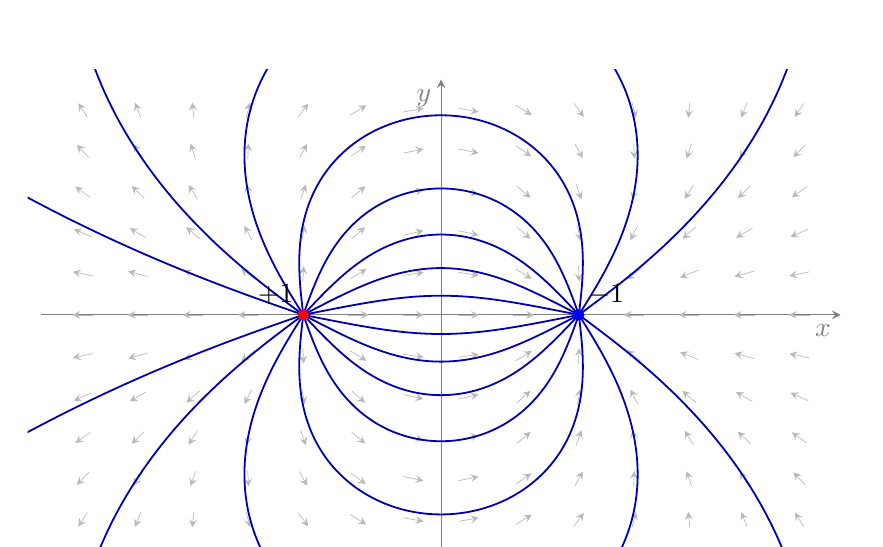
\begin{tikzpicture}[x=1.75cm,y=1.3cm,>=stealth]
\clip (-3,-2.4) rectangle (3,2.4);
\draw[gray,->] (-2.9,0)--(2.9,0) node[below left]{$x$};
\draw[gray,->] (0,-2.3)--(0,2.3) node[below left]{$y$};
\draw[gray!55,->,line width=.25pt](-2.5674,-1.9325)--(-2.6326,-2.0675);
\draw[gray!55,->,line width=.25pt](-2.5567,-1.5388)--(-2.6433,-1.6612);
\draw[gray!55,->,line width=.25pt](-2.5458,-1.1482)--(-2.6542,-1.2518);
\draw[gray!55,->,line width=.25pt](-2.5356,-0.7616)--(-2.6644,-0.8384);
\draw[gray!55,->,line width=.25pt](-2.5279,-0.3793)--(-2.6721,-0.4207);
\draw[gray!55,->,line width=.25pt](-2.5250,-0.0000)--(-2.6750,-0.0000);
\draw[gray!55,->,line width=.25pt](-2.5279,0.3793)--(-2.6721,0.4207);
\draw[gray!55,->,line width=.25pt](-2.5356,0.7616)--(-2.6644,0.8384);
\draw[gray!55,->,line width=.25pt](-2.5458,1.1482)--(-2.6542,1.2518);
\draw[gray!55,->,line width=.25pt](-2.5567,1.5388)--(-2.6433,1.6612);
\draw[gray!55,->,line width=.25pt](-2.5674,1.9325)--(-2.6326,2.0675);
\draw[gray!55,->,line width=.25pt](-2.1791,-1.9280)--(-2.2209,-2.0720);
\draw[gray!55,->,line width=.25pt](-2.1672,-1.5325)--(-2.2328,-1.6675);
\draw[gray!55,->,line width=.25pt](-2.1543,-1.1405)--(-2.2457,-1.2595);
\draw[gray!55,->,line width=.25pt](-2.1410,-0.7536)--(-2.2590,-0.8464);
\draw[gray!55,->,line width=.25pt](-2.1297,-0.3738)--(-2.2703,-0.4262);
\draw[gray!55,->,line width=.25pt](-2.1250,-0.0000)--(-2.2750,-0.0000);
\draw[gray!55,->,line width=.25pt](-2.1297,0.3738)--(-2.2703,0.4262);
\draw[gray!55,->,line width=.25pt](-2.1410,0.7536)--(-2.2590,0.8464);
\draw[gray!55,->,line width=.25pt](-2.1543,1.1405)--(-2.2457,1.2595);
\draw[gray!55,->,line width=.25pt](-2.1672,1.5325)--(-2.2328,1.6675);
\draw[gray!55,->,line width=.25pt](-2.1791,1.9280)--(-2.2209,2.0720);
\draw[gray!55,->,line width=.25pt](-1.7944,-1.9252)--(-1.8056,-2.0748);
\draw[gray!55,->,line width=.25pt](-1.7823,-1.5271)--(-1.8177,-1.6729);
\draw[gray!55,->,line width=.25pt](-1.7682,-1.1321)--(-1.8318,-1.2679);
\draw[gray!55,->,line width=.25pt](-1.7516,-0.7427)--(-1.8484,-0.8573);
\draw[gray!55,->,line width=.25pt](-1.7341,-0.3641)--(-1.8659,-0.4359);
\draw[gray!55,->,line width=.25pt](-1.7250,-0.0000)--(-1.8750,-0.0000);
\draw[gray!55,->,line width=.25pt](-1.7341,0.3641)--(-1.8659,0.4359);
\draw[gray!55,->,line width=.25pt](-1.7516,0.7427)--(-1.8484,0.8573);
\draw[gray!55,->,line width=.25pt](-1.7682,1.1321)--(-1.8318,1.2679);
\draw[gray!55,->,line width=.25pt](-1.7823,1.5271)--(-1.8177,1.6729);
\draw[gray!55,->,line width=.25pt](-1.7944,1.9252)--(-1.8056,2.0748);
\draw[gray!55,->,line width=.25pt](-1.4137,-1.9263)--(-1.3863,-2.0737);
\draw[gray!55,->,line width=.25pt](-1.4028,-1.5251)--(-1.3972,-1.6749);
\draw[gray!55,->,line width=.25pt](-1.3897,-1.1257)--(-1.4103,-1.2743);
\draw[gray!55,->,line width=.25pt](-1.3731,-0.7300)--(-1.4269,-0.8700);
\draw[gray!55,->,line width=.25pt](-1.3487,-0.3453)--(-1.4513,-0.4547);
\draw[gray!55,->,line width=.25pt](-1.3250,-0.0000)--(-1.4750,-0.0000);
\draw[gray!55,->,line width=.25pt](-1.3487,0.3453)--(-1.4513,0.4547);
\draw[gray!55,->,line width=.25pt](-1.3731,0.7300)--(-1.4269,0.8700);
\draw[gray!55,->,line width=.25pt](-1.3897,1.1257)--(-1.4103,1.2743);
\draw[gray!55,->,line width=.25pt](-1.4028,1.5251)--(-1.3972,1.6749);
\draw[gray!55,->,line width=.25pt](-1.4137,1.9263)--(-1.3863,2.0737);
\draw[gray!55,->,line width=.25pt](-1.0360,-1.9342)--(-0.9640,-2.0658);
\draw[gray!55,->,line width=.25pt](-1.0280,-1.5304)--(-0.9720,-1.6696);
\draw[gray!55,->,line width=.25pt](-1.0191,-1.1275)--(-0.9809,-1.2725);
\draw[gray!55,->,line width=.25pt](-1.0100,-0.7257)--(-0.9900,-0.8743);
\draw[gray!55,->,line width=.25pt](-1.0028,-0.3251)--(-0.9972,-0.4749);
\draw[gray!55,->,line width=.25pt](-1.0028,0.3251)--(-0.9972,0.4749);
\draw[gray!55,->,line width=.25pt](-1.0100,0.7257)--(-0.9900,0.8743);
\draw[gray!55,->,line width=.25pt](-1.0191,1.1275)--(-0.9809,1.2725);
\draw[gray!55,->,line width=.25pt](-1.0280,1.5304)--(-0.9720,1.6696);
\draw[gray!55,->,line width=.25pt](-1.0360,1.9342)--(-0.9640,2.0658);
\draw[gray!55,->,line width=.25pt](-0.6580,-1.9525)--(-0.5420,-2.0475);
\draw[gray!55,->,line width=.25pt](-0.6541,-1.5480)--(-0.5459,-1.6520);
\draw[gray!55,->,line width=.25pt](-0.6501,-1.1442)--(-0.5499,-1.2558);
\draw[gray!55,->,line width=.25pt](-0.6488,-0.7431)--(-0.5512,-0.8569);
\draw[gray!55,->,line width=.25pt](-0.6578,-0.3522)--(-0.5422,-0.4478);
\draw[gray!55,->,line width=.25pt](-0.6750,-0.0000)--(-0.5250,-0.0000);
\draw[gray!55,->,line width=.25pt](-0.6578,0.3522)--(-0.5422,0.4478);
\draw[gray!55,->,line width=.25pt](-0.6488,0.7431)--(-0.5512,0.8569);
\draw[gray!55,->,line width=.25pt](-0.6501,1.1442)--(-0.5499,1.2558);
\draw[gray!55,->,line width=.25pt](-0.6541,1.5480)--(-0.5459,1.6520);
\draw[gray!55,->,line width=.25pt](-0.6580,1.9525)--(-0.5420,2.0475);
\draw[gray!55,->,line width=.25pt](-0.2729,-1.9823)--(-0.1271,-2.0177);
\draw[gray!55,->,line width=.25pt](-0.2723,-1.5802)--(-0.1277,-1.6198);
\draw[gray!55,->,line width=.25pt](-0.2718,-1.1783)--(-0.1282,-1.2217);
\draw[gray!55,->,line width=.25pt](-0.2718,-0.7784)--(-0.1282,-0.8216);
\draw[gray!55,->,line width=.25pt](-0.2734,-0.3845)--(-0.1266,-0.4155);
\draw[gray!55,->,line width=.25pt](-0.2750,-0.0000)--(-0.1250,-0.0000);
\draw[gray!55,->,line width=.25pt](-0.2734,0.3845)--(-0.1266,0.4155);
\draw[gray!55,->,line width=.25pt](-0.2718,0.7784)--(-0.1282,0.8216);
\draw[gray!55,->,line width=.25pt](-0.2718,1.1783)--(-0.1282,1.2217);
\draw[gray!55,->,line width=.25pt](-0.2723,1.5802)--(-0.1277,1.6198);
\draw[gray!55,->,line width=.25pt](-0.2729,1.9823)--(-0.1271,2.0177);
\draw[gray!55,->,line width=.25pt](0.1271,-2.0177)--(0.2729,-1.9823);
\draw[gray!55,->,line width=.25pt](0.1277,-1.6198)--(0.2723,-1.5802);
\draw[gray!55,->,line width=.25pt](0.1282,-1.2217)--(0.2718,-1.1783);
\draw[gray!55,->,line width=.25pt](0.1282,-0.8216)--(0.2718,-0.7784);
\draw[gray!55,->,line width=.25pt](0.1266,-0.4155)--(0.2734,-0.3845);
\draw[gray!55,->,line width=.25pt](0.1250,-0.0000)--(0.2750,-0.0000);
\draw[gray!55,->,line width=.25pt](0.1266,0.4155)--(0.2734,0.3845);
\draw[gray!55,->,line width=.25pt](0.1282,0.8216)--(0.2718,0.7784);
\draw[gray!55,->,line width=.25pt](0.1282,1.2217)--(0.2718,1.1783);
\draw[gray!55,->,line width=.25pt](0.1277,1.6198)--(0.2723,1.5802);
\draw[gray!55,->,line width=.25pt](0.1271,2.0177)--(0.2729,1.9823);
\draw[gray!55,->,line width=.25pt](0.5420,-2.0475)--(0.6580,-1.9525);
\draw[gray!55,->,line width=.25pt](0.5459,-1.6520)--(0.6541,-1.5480);
\draw[gray!55,->,line width=.25pt](0.5499,-1.2558)--(0.6501,-1.1442);
\draw[gray!55,->,line width=.25pt](0.5512,-0.8569)--(0.6488,-0.7431);
\draw[gray!55,->,line width=.25pt](0.5422,-0.4478)--(0.6578,-0.3522);
\draw[gray!55,->,line width=.25pt](0.5250,-0.0000)--(0.6750,-0.0000);
\draw[gray!55,->,line width=.25pt](0.5422,0.4478)--(0.6578,0.3522);
\draw[gray!55,->,line width=.25pt](0.5512,0.8569)--(0.6488,0.7431);
\draw[gray!55,->,line width=.25pt](0.5499,1.2558)--(0.6501,1.1442);
\draw[gray!55,->,line width=.25pt](0.5459,1.6520)--(0.6541,1.5480);
\draw[gray!55,->,line width=.25pt](0.5420,2.0475)--(0.6580,1.9525);
\draw[gray!55,->,line width=.25pt](0.9640,-2.0658)--(1.0360,-1.9342);
\draw[gray!55,->,line width=.25pt](0.9720,-1.6696)--(1.0280,-1.5304);
\draw[gray!55,->,line width=.25pt](0.9809,-1.2725)--(1.0191,-1.1275);
\draw[gray!55,->,line width=.25pt](0.9900,-0.8743)--(1.0100,-0.7257);
\draw[gray!55,->,line width=.25pt](0.9972,-0.4749)--(1.0028,-0.3251);
\draw[gray!55,->,line width=.25pt](0.9972,0.4749)--(1.0028,0.3251);
\draw[gray!55,->,line width=.25pt](0.9900,0.8743)--(1.0100,0.7257);
\draw[gray!55,->,line width=.25pt](0.9809,1.2725)--(1.0191,1.1275);
\draw[gray!55,->,line width=.25pt](0.9720,1.6696)--(1.0280,1.5304);
\draw[gray!55,->,line width=.25pt](0.9640,2.0658)--(1.0360,1.9342);
\draw[gray!55,->,line width=.25pt](1.3863,-2.0737)--(1.4137,-1.9263);
\draw[gray!55,->,line width=.25pt](1.3972,-1.6749)--(1.4028,-1.5251);
\draw[gray!55,->,line width=.25pt](1.4103,-1.2743)--(1.3897,-1.1257);
\draw[gray!55,->,line width=.25pt](1.4269,-0.8700)--(1.3731,-0.7300);
\draw[gray!55,->,line width=.25pt](1.4513,-0.4547)--(1.3487,-0.3453);
\draw[gray!55,->,line width=.25pt](1.4750,-0.0000)--(1.3250,-0.0000);
\draw[gray!55,->,line width=.25pt](1.4513,0.4547)--(1.3487,0.3453);
\draw[gray!55,->,line width=.25pt](1.4269,0.8700)--(1.3731,0.7300);
\draw[gray!55,->,line width=.25pt](1.4103,1.2743)--(1.3897,1.1257);
\draw[gray!55,->,line width=.25pt](1.3972,1.6749)--(1.4028,1.5251);
\draw[gray!55,->,line width=.25pt](1.3863,2.0737)--(1.4137,1.9263);
\draw[gray!55,->,line width=.25pt](1.8056,-2.0748)--(1.7944,-1.9252);
\draw[gray!55,->,line width=.25pt](1.8177,-1.6729)--(1.7823,-1.5271);
\draw[gray!55,->,line width=.25pt](1.8318,-1.2679)--(1.7682,-1.1321);
\draw[gray!55,->,line width=.25pt](1.8484,-0.8573)--(1.7516,-0.7427);
\draw[gray!55,->,line width=.25pt](1.8659,-0.4359)--(1.7341,-0.3641);
\draw[gray!55,->,line width=.25pt](1.8750,-0.0000)--(1.7250,-0.0000);
\draw[gray!55,->,line width=.25pt](1.8659,0.4359)--(1.7341,0.3641);
\draw[gray!55,->,line width=.25pt](1.8484,0.8573)--(1.7516,0.7427);
\draw[gray!55,->,line width=.25pt](1.8318,1.2679)--(1.7682,1.1321);
\draw[gray!55,->,line width=.25pt](1.8177,1.6729)--(1.7823,1.5271);
\draw[gray!55,->,line width=.25pt](1.8056,2.0748)--(1.7944,1.9252);
\draw[gray!55,->,line width=.25pt](2.2209,-2.0720)--(2.1791,-1.9280);
\draw[gray!55,->,line width=.25pt](2.2328,-1.6675)--(2.1672,-1.5325);
\draw[gray!55,->,line width=.25pt](2.2457,-1.2595)--(2.1543,-1.1405);
\draw[gray!55,->,line width=.25pt](2.2590,-0.8464)--(2.1410,-0.7536);
\draw[gray!55,->,line width=.25pt](2.2703,-0.4262)--(2.1297,-0.3738);
\draw[gray!55,->,line width=.25pt](2.2750,-0.0000)--(2.1250,-0.0000);
\draw[gray!55,->,line width=.25pt](2.2703,0.4262)--(2.1297,0.3738);
\draw[gray!55,->,line width=.25pt](2.2590,0.8464)--(2.1410,0.7536);
\draw[gray!55,->,line width=.25pt](2.2457,1.2595)--(2.1543,1.1405);
\draw[gray!55,->,line width=.25pt](2.2328,1.6675)--(2.1672,1.5325);
\draw[gray!55,->,line width=.25pt](2.2209,2.0720)--(2.1791,1.9280);
\draw[gray!55,->,line width=.25pt](2.6326,-2.0675)--(2.5674,-1.9325);
\draw[gray!55,->,line width=.25pt](2.6433,-1.6612)--(2.5567,-1.5388);
\draw[gray!55,->,line width=.25pt](2.6542,-1.2518)--(2.5458,-1.1482);
\draw[gray!55,->,line width=.25pt](2.6644,-0.8384)--(2.5356,-0.7616);
\draw[gray!55,->,line width=.25pt](2.6721,-0.4207)--(2.5279,-0.3793);
\draw[gray!55,->,line width=.25pt](2.6750,-0.0000)--(2.5250,-0.0000);
\draw[gray!55,->,line width=.25pt](2.6721,0.4207)--(2.5279,0.3793);
\draw[gray!55,->,line width=.25pt](2.6644,0.8384)--(2.5356,0.7616);
\draw[gray!55,->,line width=.25pt](2.6542,1.2518)--(2.5458,1.1482);
\draw[gray!55,->,line width=.25pt](2.6433,1.6612)--(2.5567,1.5388);
\draw[gray!55,->,line width=.25pt](2.6326,2.0675)--(2.5674,1.9325);
\draw[blue!70!black,line width=.65pt] plot coordinates {(-0.97585,-0.00647) (-0.97209,-0.00748) (-0.96381,-0.00970) (-0.95430,-0.01224) (-0.94367,-0.01509) (-0.93192,-0.01823) (-0.91903,-0.02168) (-0.90500,-0.02542) (-0.88981,-0.02947) (-0.87346,-0.03382) (-0.85595,-0.03847) (-0.83728,-0.04341) (-0.81746,-0.04864) (-0.79649,-0.05415) (-0.77437,-0.05993) (-0.75112,-0.06596) (-0.72691,-0.07219) (-0.70268,-0.07836) (-0.67844,-0.08447) (-0.65418,-0.09051) (-0.62990,-0.09647) (-0.60560,-0.10234) (-0.58128,-0.10811) (-0.55692,-0.11377) (-0.53255,-0.11931) (-0.50814,-0.12472) (-0.48370,-0.12999) (-0.45923,-0.13511) (-0.43472,-0.14005) (-0.41018,-0.14482) (-0.38561,-0.14940) (-0.36099,-0.15378) (-0.33634,-0.15794) (-0.31165,-0.16186) (-0.28692,-0.16555) (-0.26216,-0.16898) (-0.23736,-0.17214) (-0.21253,-0.17503) (-0.18766,-0.17762) (-0.16277,-0.17992) (-0.13785,-0.18190) (-0.11291,-0.18357) (-0.08794,-0.18492) (-0.06296,-0.18593) (-0.03797,-0.18661) (-0.01297,-0.18696) (0.01203,-0.18697) (0.03702,-0.18663) (0.06201,-0.18596) (0.08699,-0.18496) (0.11196,-0.18363) (0.13690,-0.18197) (0.16182,-0.18000) (0.18672,-0.17771) (0.21159,-0.17513) (0.23642,-0.17226) (0.26122,-0.16910) (0.28598,-0.16568) (0.31071,-0.16201) (0.33540,-0.15809) (0.36006,-0.15394) (0.38467,-0.14957) (0.40925,-0.14500) (0.43379,-0.14024) (0.45830,-0.13530) (0.48277,-0.13019) (0.50721,-0.12492) (0.53162,-0.11952) (0.55600,-0.11398) (0.58035,-0.10832) (0.60468,-0.10256) (0.62898,-0.09669) (0.65326,-0.09074) (0.67752,-0.08470) (0.70176,-0.07860) (0.72599,-0.07242) (0.75020,-0.06620) (0.77407,-0.06001) (0.79681,-0.05407) (0.81840,-0.04840) (0.83883,-0.04301) (0.85810,-0.03790) (0.87619,-0.03310) (0.89309,-0.02860) (0.90879,-0.02441) (0.92329,-0.02054) (0.93658,-0.01699) (0.94744,-0.01408) (0.95831,-0.01117) (0.96690,-0.00887) (0.97445,-0.00685) (0.97585,-0.00647)};
\draw[blue!70!black,line width=.65pt] plot coordinates {(-0.97585,0.00647) (-0.97209,0.00748) (-0.96381,0.00970) (-0.95430,0.01224) (-0.94367,0.01509) (-0.93192,0.01823) (-0.91903,0.02168) (-0.90500,0.02542) (-0.88981,0.02947) (-0.87346,0.03382) (-0.85595,0.03847) (-0.83728,0.04341) (-0.81746,0.04864) (-0.79649,0.05415) (-0.77437,0.05993) (-0.75112,0.06596) (-0.72691,0.07219) (-0.70268,0.07836) (-0.67844,0.08447) (-0.65418,0.09051) (-0.62990,0.09647) (-0.60560,0.10234) (-0.58128,0.10811) (-0.55692,0.11377) (-0.53255,0.11931) (-0.50814,0.12472) (-0.48370,0.12999) (-0.45923,0.13511) (-0.43472,0.14005) (-0.41018,0.14482) (-0.38561,0.14940) (-0.36099,0.15378) (-0.33634,0.15794) (-0.31165,0.16186) (-0.28692,0.16555) (-0.26216,0.16898) (-0.23736,0.17214) (-0.21253,0.17503) (-0.18766,0.17762) (-0.16277,0.17992) (-0.13785,0.18190) (-0.11291,0.18357) (-0.08794,0.18492) (-0.06296,0.18593) (-0.03797,0.18661) (-0.01297,0.18696) (0.01203,0.18697) (0.03702,0.18663) (0.06201,0.18596) (0.08699,0.18496) (0.11196,0.18363) (0.13690,0.18197) (0.16182,0.18000) (0.18672,0.17771) (0.21159,0.17513) (0.23642,0.17226) (0.26122,0.16910) (0.28598,0.16568) (0.31071,0.16201) (0.33540,0.15809) (0.36006,0.15394) (0.38467,0.14957) (0.40925,0.14500) (0.43379,0.14024) (0.45830,0.13530) (0.48277,0.13019) (0.50721,0.12492) (0.53162,0.11952) (0.55600,0.11398) (0.58035,0.10832) (0.60468,0.10256) (0.62898,0.09669) (0.65326,0.09074) (0.67752,0.08470) (0.70176,0.07860) (0.72599,0.07242) (0.75020,0.06620) (0.77407,0.06001) (0.79681,0.05407) (0.81840,0.04840) (0.83883,0.04301) (0.85810,0.03790) (0.87619,0.03310) (0.89309,0.02860) (0.90879,0.02441) (0.92329,0.02054) (0.93658,0.01699) (0.94744,0.01408) (0.95831,0.01117) (0.96690,0.00887) (0.97445,0.00685) (0.97585,0.00647)};
\draw[blue!70!black,line width=.65pt] plot coordinates {(-0.97952,-0.01434) (-0.97658,-0.01640) (-0.96988,-0.02108) (-0.96214,-0.02650) (-0.95343,-0.03260) (-0.94372,-0.03938) (-0.93300,-0.04687) (-0.92124,-0.05507) (-0.90843,-0.06399) (-0.89456,-0.07363) (-0.87959,-0.08401) (-0.86354,-0.09510) (-0.84638,-0.10691) (-0.82811,-0.11942) (-0.80871,-0.13262) (-0.78818,-0.14649) (-0.76741,-0.16040) (-0.74657,-0.17422) (-0.72566,-0.18792) (-0.70467,-0.20150) (-0.68360,-0.21495) (-0.66242,-0.22824) (-0.64115,-0.24137) (-0.61976,-0.25431) (-0.59825,-0.26705) (-0.57661,-0.27957) (-0.55484,-0.29186) (-0.53292,-0.30388) (-0.51085,-0.31563) (-0.48863,-0.32708) (-0.46624,-0.33820) (-0.44368,-0.34898) (-0.42095,-0.35939) (-0.39805,-0.36941) (-0.37496,-0.37900) (-0.35170,-0.38816) (-0.32826,-0.39685) (-0.30464,-0.40504) (-0.28085,-0.41272) (-0.25689,-0.41986) (-0.23277,-0.42642) (-0.20850,-0.43240) (-0.18408,-0.43777) (-0.15953,-0.44251) (-0.13487,-0.44660) (-0.11011,-0.45002) (-0.08526,-0.45277) (-0.06034,-0.45482) (-0.03538,-0.45618) (-0.01039,-0.45682) (0.01461,-0.45676) (0.03960,-0.45600) (0.06455,-0.45452) (0.08946,-0.45235) (0.11429,-0.44949) (0.13904,-0.44596) (0.16368,-0.44176) (0.18821,-0.43691) (0.21260,-0.43144) (0.23685,-0.42536) (0.26094,-0.41869) (0.28487,-0.41146) (0.30864,-0.40370) (0.33223,-0.39542) (0.35564,-0.38665) (0.37887,-0.37742) (0.40192,-0.36774) (0.42480,-0.35766) (0.44750,-0.34719) (0.47003,-0.33635) (0.49239,-0.32517) (0.51458,-0.31367) (0.53663,-0.30187) (0.55852,-0.28980) (0.58027,-0.27748) (0.60189,-0.26492) (0.62337,-0.25214) (0.64474,-0.23917) (0.66600,-0.22601) (0.68716,-0.21269) (0.70822,-0.19922) (0.72920,-0.18562) (0.75009,-0.17189) (0.77092,-0.15806) (0.79168,-0.14414) (0.81239,-0.13013) (0.83227,-0.11657) (0.85102,-0.10372) (0.86863,-0.09158) (0.88511,-0.08018) (0.90046,-0.06953) (0.91468,-0.05964) (0.92778,-0.05051) (0.93976,-0.04215) (0.94954,-0.03531) (0.95932,-0.02848) (0.96707,-0.02306) (0.97391,-0.01826) (0.97952,-0.01434)};
\draw[blue!70!black,line width=.65pt] plot coordinates {(-0.97952,0.01434) (-0.97658,0.01640) (-0.96988,0.02108) (-0.96214,0.02650) (-0.95343,0.03260) (-0.94372,0.03938) (-0.93300,0.04687) (-0.92124,0.05507) (-0.90843,0.06399) (-0.89456,0.07363) (-0.87959,0.08401) (-0.86354,0.09510) (-0.84638,0.10691) (-0.82811,0.11942) (-0.80871,0.13262) (-0.78818,0.14649) (-0.76741,0.16040) (-0.74657,0.17422) (-0.72566,0.18792) (-0.70467,0.20150) (-0.68360,0.21495) (-0.66242,0.22824) (-0.64115,0.24137) (-0.61976,0.25431) (-0.59825,0.26705) (-0.57661,0.27957) (-0.55484,0.29186) (-0.53292,0.30388) (-0.51085,0.31563) (-0.48863,0.32708) (-0.46624,0.33820) (-0.44368,0.34898) (-0.42095,0.35939) (-0.39805,0.36941) (-0.37496,0.37900) (-0.35170,0.38816) (-0.32826,0.39685) (-0.30464,0.40504) (-0.28085,0.41272) (-0.25689,0.41986) (-0.23277,0.42642) (-0.20850,0.43240) (-0.18408,0.43777) (-0.15953,0.44251) (-0.13487,0.44660) (-0.11011,0.45002) (-0.08526,0.45277) (-0.06034,0.45482) (-0.03538,0.45618) (-0.01039,0.45682) (0.01461,0.45676) (0.03960,0.45600) (0.06455,0.45452) (0.08946,0.45235) (0.11429,0.44949) (0.13904,0.44596) (0.16368,0.44176) (0.18821,0.43691) (0.21260,0.43144) (0.23685,0.42536) (0.26094,0.41869) (0.28487,0.41146) (0.30864,0.40370) (0.33223,0.39542) (0.35564,0.38665) (0.37887,0.37742) (0.40192,0.36774) (0.42480,0.35766) (0.44750,0.34719) (0.47003,0.33635) (0.49239,0.32517) (0.51458,0.31367) (0.53663,0.30187) (0.55852,0.28980) (0.58027,0.27748) (0.60189,0.26492) (0.62337,0.25214) (0.64474,0.23917) (0.66600,0.22601) (0.68716,0.21269) (0.70822,0.19922) (0.72920,0.18562) (0.75009,0.17189) (0.77092,0.15806) (0.79168,0.14414) (0.81239,0.13013) (0.83227,0.11657) (0.85102,0.10372) (0.86863,0.09158) (0.88511,0.08018) (0.90046,0.06953) (0.91468,0.05964) (0.92778,0.05051) (0.93976,0.04215) (0.94954,0.03531) (0.95932,0.02848) (0.96707,0.02306) (0.97391,0.01826) (0.97952,0.01434)};
\draw[blue!70!black,line width=.65pt] plot coordinates {(-0.98566,-0.02048) (-0.98365,-0.02335) (-0.97874,-0.03036) (-0.97297,-0.03858) (-0.96643,-0.04792) (-0.95906,-0.05840) (-0.95086,-0.07007) (-0.94179,-0.08294) (-0.93184,-0.09704) (-0.92096,-0.11239) (-0.90916,-0.12899) (-0.89639,-0.14685) (-0.88264,-0.16595) (-0.86797,-0.18619) (-0.85320,-0.20636) (-0.83833,-0.22646) (-0.82335,-0.24648) (-0.80825,-0.26640) (-0.79300,-0.28621) (-0.77761,-0.30591) (-0.76206,-0.32549) (-0.74633,-0.34492) (-0.73041,-0.36420) (-0.71430,-0.38331) (-0.69797,-0.40224) (-0.68141,-0.42097) (-0.66462,-0.43949) (-0.64757,-0.45778) (-0.63027,-0.47582) (-0.61269,-0.49360) (-0.59483,-0.51109) (-0.57667,-0.52827) (-0.55821,-0.54513) (-0.53944,-0.56164) (-0.52034,-0.57778) (-0.50092,-0.59352) (-0.48116,-0.60883) (-0.46107,-0.62370) (-0.44063,-0.63810) (-0.41984,-0.65199) (-0.39871,-0.66535) (-0.37724,-0.67815) (-0.35543,-0.69037) (-0.33328,-0.70196) (-0.31081,-0.71291) (-0.28802,-0.72319) (-0.26492,-0.73275) (-0.24154,-0.74159) (-0.21788,-0.74966) (-0.19397,-0.75695) (-0.16982,-0.76343) (-0.14547,-0.76908) (-0.12093,-0.77387) (-0.09624,-0.77779) (-0.07143,-0.78083) (-0.04652,-0.78298) (-0.02156,-0.78422) (0.00344,-0.78455) (0.02843,-0.78397) (0.05339,-0.78248) (0.07827,-0.78009) (0.10305,-0.77680) (0.12770,-0.77264) (0.15219,-0.76761) (0.17649,-0.76173) (0.20057,-0.75503) (0.22442,-0.74752) (0.24800,-0.73923) (0.27131,-0.73019) (0.29432,-0.72043) (0.31703,-0.70997) (0.33941,-0.69884) (0.36146,-0.68707) (0.38318,-0.67469) (0.40456,-0.66173) (0.42560,-0.64822) (0.44629,-0.63418) (0.46663,-0.61966) (0.48663,-0.60466) (0.50630,-0.58923) (0.52563,-0.57338) (0.54464,-0.55713) (0.56332,-0.54053) (0.58170,-0.52358) (0.59977,-0.50631) (0.61756,-0.48873) (0.63506,-0.47088) (0.65229,-0.45277) (0.66926,-0.43442) (0.68599,-0.41584) (0.70248,-0.39705) (0.71875,-0.37807) (0.73481,-0.35891) (0.75067,-0.33958) (0.76635,-0.32011) (0.78186,-0.30050) (0.79721,-0.28077) (0.81242,-0.26093) (0.82748,-0.24098) (0.84243,-0.22094) (0.85727,-0.20082) (0.87201,-0.18063) (0.88667,-0.16037) (0.90082,-0.14066) (0.91397,-0.12224) (0.92611,-0.10513) (0.93727,-0.08935) (0.94746,-0.07490) (0.95577,-0.06309) (0.96407,-0.05127) (0.97066,-0.04188) (0.97649,-0.03357) (0.98158,-0.02631) (0.98566,-0.02048)};
\draw[blue!70!black,line width=.65pt] plot coordinates {(-0.98566,0.02048) (-0.98365,0.02335) (-0.97874,0.03036) (-0.97297,0.03858) (-0.96643,0.04792) (-0.95906,0.05840) (-0.95086,0.07007) (-0.94179,0.08294) (-0.93184,0.09704) (-0.92096,0.11239) (-0.90916,0.12899) (-0.89639,0.14685) (-0.88264,0.16595) (-0.86797,0.18619) (-0.85320,0.20636) (-0.83833,0.22646) (-0.82335,0.24648) (-0.80825,0.26640) (-0.79300,0.28621) (-0.77761,0.30591) (-0.76206,0.32549) (-0.74633,0.34492) (-0.73041,0.36420) (-0.71430,0.38331) (-0.69797,0.40224) (-0.68141,0.42097) (-0.66462,0.43949) (-0.64757,0.45778) (-0.63027,0.47582) (-0.61269,0.49360) (-0.59483,0.51109) (-0.57667,0.52827) (-0.55821,0.54513) (-0.53944,0.56164) (-0.52034,0.57778) (-0.50092,0.59352) (-0.48116,0.60883) (-0.46107,0.62370) (-0.44063,0.63810) (-0.41984,0.65199) (-0.39871,0.66535) (-0.37724,0.67815) (-0.35543,0.69037) (-0.33328,0.70196) (-0.31081,0.71291) (-0.28802,0.72319) (-0.26492,0.73275) (-0.24154,0.74159) (-0.21788,0.74966) (-0.19397,0.75695) (-0.16982,0.76343) (-0.14547,0.76908) (-0.12093,0.77387) (-0.09624,0.77779) (-0.07143,0.78083) (-0.04652,0.78298) (-0.02156,0.78422) (0.00344,0.78455) (0.02843,0.78397) (0.05339,0.78248) (0.07827,0.78009) (0.10305,0.77680) (0.12770,0.77264) (0.15219,0.76761) (0.17649,0.76173) (0.20057,0.75503) (0.22442,0.74752) (0.24800,0.73923) (0.27131,0.73019) (0.29432,0.72043) (0.31703,0.70997) (0.33941,0.69884) (0.36146,0.68707) (0.38318,0.67469) (0.40456,0.66173) (0.42560,0.64822) (0.44629,0.63418) (0.46663,0.61966) (0.48663,0.60466) (0.50630,0.58923) (0.52563,0.57338) (0.54464,0.55713) (0.56332,0.54053) (0.58170,0.52358) (0.59977,0.50631) (0.61756,0.48873) (0.63506,0.47088) (0.65229,0.45277) (0.66926,0.43442) (0.68599,0.41584) (0.70248,0.39705) (0.71875,0.37807) (0.73481,0.35891) (0.75067,0.33958) (0.76635,0.32011) (0.78186,0.30050) (0.79721,0.28077) (0.81242,0.26093) (0.82748,0.24098) (0.84243,0.22094) (0.85727,0.20082) (0.87201,0.18063) (0.88667,0.16037) (0.90082,0.14066) (0.91397,0.12224) (0.92611,0.10513) (0.93727,0.08935) (0.94746,0.07490) (0.95577,0.06309) (0.96407,0.05127) (0.97066,0.04188) (0.97649,0.03357) (0.98158,0.02631) (0.98566,0.02048)};
\draw[blue!70!black,line width=.65pt] plot coordinates {(-0.99353,-0.02415) (-0.99263,-0.02750) (-0.99005,-0.03712) (-0.98694,-0.04870) (-0.98333,-0.06210) (-0.97921,-0.07738) (-0.97454,-0.09459) (-0.96932,-0.11376) (-0.96351,-0.13491) (-0.95710,-0.15804) (-0.95034,-0.18211) (-0.94350,-0.20615) (-0.93655,-0.23017) (-0.92950,-0.25415) (-0.92231,-0.27810) (-0.91499,-0.30200) (-0.90752,-0.32586) (-0.89988,-0.34966) (-0.89207,-0.37341) (-0.88407,-0.39710) (-0.87587,-0.42071) (-0.86746,-0.44426) (-0.85882,-0.46772) (-0.84994,-0.49109) (-0.84082,-0.51436) (-0.83144,-0.53753) (-0.82178,-0.56059) (-0.81184,-0.58353) (-0.80160,-0.60634) (-0.79106,-0.62901) (-0.78020,-0.65153) (-0.76901,-0.67388) (-0.75748,-0.69607) (-0.74561,-0.71807) (-0.73338,-0.73987) (-0.72078,-0.76146) (-0.70780,-0.78283) (-0.69443,-0.80396) (-0.68068,-0.82483) (-0.66652,-0.84543) (-0.65195,-0.86575) (-0.63696,-0.88576) (-0.62155,-0.90544) (-0.60572,-0.92479) (-0.58945,-0.94377) (-0.57275,-0.96237) (-0.55561,-0.98057) (-0.53802,-0.99834) (-0.52000,-1.01566) (-0.50153,-1.03251) (-0.48263,-1.04887) (-0.46328,-1.06470) (-0.44350,-1.07999) (-0.42330,-1.09471) (-0.40267,-1.10884) (-0.38163,-1.12234) (-0.36019,-1.13519) (-0.33836,-1.14738) (-0.31615,-1.15886) (-0.29359,-1.16962) (-0.27068,-1.17963) (-0.24746,-1.18887) (-0.22393,-1.19732) (-0.20012,-1.20495) (-0.17607,-1.21175) (-0.15178,-1.21770) (-0.12731,-1.22277) (-0.10266,-1.22697) (-0.07788,-1.23027) (-0.05300,-1.23266) (-0.02804,-1.23415) (-0.00305,-1.23472) (0.02194,-1.23437) (0.04691,-1.23311) (0.07181,-1.23094) (0.09662,-1.22786) (0.12130,-1.22388) (0.14582,-1.21902) (0.17016,-1.21328) (0.19427,-1.20669) (0.21814,-1.19926) (0.24174,-1.19101) (0.26504,-1.18196) (0.28803,-1.17213) (0.31068,-1.16155) (0.33297,-1.15025) (0.35490,-1.13823) (0.37643,-1.12554) (0.39757,-1.11219) (0.41830,-1.09822) (0.43861,-1.08364) (0.45849,-1.06849) (0.47794,-1.05278) (0.49696,-1.03655) (0.51553,-1.01982) (0.53366,-1.00261) (0.55135,-0.98495) (0.56860,-0.96685) (0.58541,-0.94835) (0.60179,-0.92946) (0.61773,-0.91020) (0.63324,-0.89059) (0.64833,-0.87066) (0.66300,-0.85042) (0.67726,-0.82988) (0.69111,-0.80908) (0.70457,-0.78801) (0.71764,-0.76670) (0.73033,-0.74516) (0.74266,-0.72341) (0.75462,-0.70146) (0.76623,-0.67932) (0.77750,-0.65700) (0.78844,-0.63452) (0.79906,-0.61189) (0.80937,-0.58911) (0.81938,-0.56621) (0.82910,-0.54318) (0.83855,-0.52003) (0.84774,-0.49678) (0.85667,-0.47343) (0.86537,-0.44999) (0.87384,-0.42647) (0.88209,-0.40287) (0.89014,-0.37920) (0.89799,-0.35547) (0.90567,-0.33168) (0.91318,-0.30783) (0.92054,-0.28394) (0.92776,-0.26000) (0.93484,-0.23603) (0.94181,-0.21202) (0.94868,-0.18798) (0.95546,-0.16392) (0.96215,-0.13983) (0.96851,-0.11672) (0.97367,-0.09779) (0.97881,-0.07886) (0.98284,-0.06392) (0.98638,-0.05077) (0.98944,-0.03940) (0.99204,-0.02971) (0.99353,-0.02415)};
\draw[blue!70!black,line width=.65pt] plot coordinates {(-0.99353,0.02415) (-0.99263,0.02750) (-0.99005,0.03712) (-0.98694,0.04870) (-0.98333,0.06210) (-0.97921,0.07738) (-0.97454,0.09459) (-0.96932,0.11376) (-0.96351,0.13491) (-0.95710,0.15804) (-0.95034,0.18211) (-0.94350,0.20615) (-0.93655,0.23017) (-0.92950,0.25415) (-0.92231,0.27810) (-0.91499,0.30200) (-0.90752,0.32586) (-0.89988,0.34966) (-0.89207,0.37341) (-0.88407,0.39710) (-0.87587,0.42071) (-0.86746,0.44426) (-0.85882,0.46772) (-0.84994,0.49109) (-0.84082,0.51436) (-0.83144,0.53753) (-0.82178,0.56059) (-0.81184,0.58353) (-0.80160,0.60634) (-0.79106,0.62901) (-0.78020,0.65153) (-0.76901,0.67388) (-0.75748,0.69607) (-0.74561,0.71807) (-0.73338,0.73987) (-0.72078,0.76146) (-0.70780,0.78283) (-0.69443,0.80396) (-0.68068,0.82483) (-0.66652,0.84543) (-0.65195,0.86575) (-0.63696,0.88576) (-0.62155,0.90544) (-0.60572,0.92479) (-0.58945,0.94377) (-0.57275,0.96237) (-0.55561,0.98057) (-0.53802,0.99834) (-0.52000,1.01566) (-0.50153,1.03251) (-0.48263,1.04887) (-0.46328,1.06470) (-0.44350,1.07999) (-0.42330,1.09471) (-0.40267,1.10884) (-0.38163,1.12234) (-0.36019,1.13519) (-0.33836,1.14738) (-0.31615,1.15886) (-0.29359,1.16962) (-0.27068,1.17963) (-0.24746,1.18887) (-0.22393,1.19732) (-0.20012,1.20495) (-0.17607,1.21175) (-0.15178,1.21770) (-0.12731,1.22277) (-0.10266,1.22697) (-0.07788,1.23027) (-0.05300,1.23266) (-0.02804,1.23415) (-0.00305,1.23472) (0.02194,1.23437) (0.04691,1.23311) (0.07181,1.23094) (0.09662,1.22786) (0.12130,1.22388) (0.14582,1.21902) (0.17016,1.21328) (0.19427,1.20669) (0.21814,1.19926) (0.24174,1.19101) (0.26504,1.18196) (0.28803,1.17213) (0.31068,1.16155) (0.33297,1.15025) (0.35490,1.13823) (0.37643,1.12554) (0.39757,1.11219) (0.41830,1.09822) (0.43861,1.08364) (0.45849,1.06849) (0.47794,1.05278) (0.49696,1.03655) (0.51553,1.01982) (0.53366,1.00261) (0.55135,0.98495) (0.56860,0.96685) (0.58541,0.94835) (0.60179,0.92946) (0.61773,0.91020) (0.63324,0.89059) (0.64833,0.87066) (0.66300,0.85042) (0.67726,0.82988) (0.69111,0.80908) (0.70457,0.78801) (0.71764,0.76670) (0.73033,0.74516) (0.74266,0.72341) (0.75462,0.70146) (0.76623,0.67932) (0.77750,0.65700) (0.78844,0.63452) (0.79906,0.61189) (0.80937,0.58911) (0.81938,0.56621) (0.82910,0.54318) (0.83855,0.52003) (0.84774,0.49678) (0.85667,0.47343) (0.86537,0.44999) (0.87384,0.42647) (0.88209,0.40287) (0.89014,0.37920) (0.89799,0.35547) (0.90567,0.33168) (0.91318,0.30783) (0.92054,0.28394) (0.92776,0.26000) (0.93484,0.23603) (0.94181,0.21202) (0.94868,0.18798) (0.95546,0.16392) (0.96215,0.13983) (0.96851,0.11672) (0.97367,0.09779) (0.97881,0.07886) (0.98284,0.06392) (0.98638,0.05077) (0.98944,0.03940) (0.99204,0.02971) (0.99353,0.02415)};
\draw[blue!70!black,line width=.65pt] plot coordinates {(-1.00218,-0.02490) (-1.00248,-0.02835) (-1.00354,-0.04053) (-1.00485,-0.05563) (-1.00637,-0.07333) (-1.00809,-0.09359) (-1.00999,-0.11634) (-1.01202,-0.14126) (-1.01398,-0.16618) (-1.01587,-0.19111) (-1.01768,-0.21604) (-1.01939,-0.24098) (-1.02099,-0.26593) (-1.02248,-0.29089) (-1.02384,-0.31585) (-1.02507,-0.34082) (-1.02616,-0.36580) (-1.02709,-0.39078) (-1.02786,-0.41577) (-1.02846,-0.44076) (-1.02888,-0.46576) (-1.02911,-0.49075) (-1.02914,-0.51575) (-1.02897,-0.54075) (-1.02859,-0.56575) (-1.02799,-0.59074) (-1.02716,-0.61573) (-1.02610,-0.64071) (-1.02479,-0.66567) (-1.02323,-0.69062) (-1.02141,-0.71556) (-1.01933,-0.74047) (-1.01698,-0.76536) (-1.01435,-0.79022) (-1.01144,-0.81505) (-1.00824,-0.83984) (-1.00473,-0.86460) (-1.00093,-0.88931) (-0.99681,-0.91396) (-0.99238,-0.93857) (-0.98762,-0.96311) (-0.98254,-0.98759) (-0.97712,-1.01200) (-0.97137,-1.03632) (-0.96526,-1.06057) (-0.95881,-1.08472) (-0.95200,-1.10877) (-0.94483,-1.13272) (-0.93729,-1.15656) (-0.92938,-1.18028) (-0.92110,-1.20386) (-0.91243,-1.22731) (-0.90338,-1.25062) (-0.89394,-1.27376) (-0.88411,-1.29675) (-0.87388,-1.31956) (-0.86324,-1.34218) (-0.85220,-1.36461) (-0.84076,-1.38684) (-0.82890,-1.40885) (-0.81662,-1.43063) (-0.80394,-1.45217) (-0.79083,-1.47345) (-0.77730,-1.49448) (-0.76334,-1.51522) (-0.74897,-1.53567) (-0.73417,-1.55582) (-0.71895,-1.57565) (-0.70330,-1.59515) (-0.68722,-1.61429) (-0.67073,-1.63308) (-0.65381,-1.65149) (-0.63648,-1.66950) (-0.61873,-1.68710) (-0.60056,-1.70428) (-0.58199,-1.72102) (-0.56302,-1.73729) (-0.54365,-1.75310) (-0.52389,-1.76841) (-0.50374,-1.78321) (-0.48322,-1.79749) (-0.46233,-1.81122) (-0.44109,-1.82440) (-0.41949,-1.83700) (-0.39757,-1.84901) (-0.37532,-1.86041) (-0.35276,-1.87119) (-0.32992,-1.88133) (-0.30679,-1.89082) (-0.28340,-1.89964) (-0.25976,-1.90778) (-0.23590,-1.91523) (-0.21182,-1.92198) (-0.18756,-1.92801) (-0.16313,-1.93331) (-0.13856,-1.93789) (-0.11385,-1.94172) (-0.08904,-1.94480) (-0.06415,-1.94713) (-0.03920,-1.94870) (-0.01422,-1.94952) (0.01078,-1.94957) (0.03577,-1.94886) (0.06072,-1.94739) (0.08562,-1.94517) (0.11045,-1.94219) (0.13516,-1.93846) (0.15976,-1.93399) (0.18421,-1.92878) (0.20850,-1.92285) (0.23260,-1.91620) (0.25649,-1.90885) (0.28016,-1.90080) (0.30358,-1.89207) (0.32675,-1.88268) (0.34964,-1.87262) (0.37224,-1.86193) (0.39453,-1.85061) (0.41650,-1.83869) (0.43813,-1.82617) (0.45943,-1.81307) (0.48037,-1.79941) (0.50094,-1.78521) (0.52114,-1.77047) (0.54095,-1.75523) (0.56038,-1.73950) (0.57941,-1.72328) (0.59803,-1.70661) (0.61625,-1.68949) (0.63406,-1.67195) (0.65145,-1.65399) (0.66843,-1.63563) (0.68498,-1.61690) (0.70111,-1.59780) (0.71682,-1.57835) (0.73210,-1.55857) (0.74696,-1.53846) (0.76139,-1.51805) (0.77540,-1.49735) (0.78899,-1.47636) (0.80216,-1.45511) (0.81490,-1.43361) (0.82723,-1.41186) (0.83915,-1.38988) (0.85065,-1.36768) (0.86175,-1.34528) (0.87244,-1.32268) (0.88272,-1.29990) (0.89261,-1.27694) (0.90211,-1.25381) (0.91121,-1.23053) (0.91993,-1.20710) (0.92827,-1.18353) (0.93623,-1.15983) (0.94382,-1.13601) (0.95104,-1.11208) (0.95789,-1.08803) (0.96440,-1.06390) (0.97055,-1.03966) (0.97635,-1.01535) (0.98182,-0.99095) (0.98694,-0.96648) (0.99174,-0.94195) (0.99622,-0.91735) (1.00038,-0.89270) (1.00423,-0.86800) (1.00777,-0.84325) (1.01102,-0.81846) (1.01397,-0.79364) (1.01664,-0.76878) (1.01903,-0.74390) (1.02114,-0.71899) (1.02300,-0.69406) (1.02459,-0.66911) (1.02593,-0.64414) (1.02703,-0.61917) (1.02789,-0.59418) (1.02852,-0.56919) (1.02893,-0.54419) (1.02913,-0.51919) (1.02912,-0.49419) (1.02892,-0.46920) (1.02853,-0.44420) (1.02795,-0.41921) (1.02720,-0.39422) (1.02629,-0.36923) (1.02523,-0.34426) (1.02402,-0.31928) (1.02267,-0.29432) (1.02120,-0.26936) (1.01961,-0.24442) (1.01792,-0.21947) (1.01613,-0.19454) (1.01425,-0.16961) (1.01229,-0.14468) (1.01027,-0.11977) (1.00844,-0.09766) (1.00676,-0.07786) (1.00527,-0.06046) (1.00397,-0.04549) (1.00288,-0.03295) (1.00218,-0.02490)};
\draw[blue!70!black,line width=.65pt] plot coordinates {(-1.00218,0.02490) (-1.00248,0.02835) (-1.00354,0.04053) (-1.00485,0.05563) (-1.00637,0.07333) (-1.00809,0.09359) (-1.00999,0.11634) (-1.01202,0.14126) (-1.01398,0.16618) (-1.01587,0.19111) (-1.01768,0.21604) (-1.01939,0.24098) (-1.02099,0.26593) (-1.02248,0.29089) (-1.02384,0.31585) (-1.02507,0.34082) (-1.02616,0.36580) (-1.02709,0.39078) (-1.02786,0.41577) (-1.02846,0.44076) (-1.02888,0.46576) (-1.02911,0.49075) (-1.02914,0.51575) (-1.02897,0.54075) (-1.02859,0.56575) (-1.02799,0.59074) (-1.02716,0.61573) (-1.02610,0.64071) (-1.02479,0.66567) (-1.02323,0.69062) (-1.02141,0.71556) (-1.01933,0.74047) (-1.01698,0.76536) (-1.01435,0.79022) (-1.01144,0.81505) (-1.00824,0.83984) (-1.00473,0.86460) (-1.00093,0.88931) (-0.99681,0.91396) (-0.99238,0.93857) (-0.98762,0.96311) (-0.98254,0.98759) (-0.97712,1.01200) (-0.97137,1.03632) (-0.96526,1.06057) (-0.95881,1.08472) (-0.95200,1.10877) (-0.94483,1.13272) (-0.93729,1.15656) (-0.92938,1.18028) (-0.92110,1.20386) (-0.91243,1.22731) (-0.90338,1.25062) (-0.89394,1.27376) (-0.88411,1.29675) (-0.87388,1.31956) (-0.86324,1.34218) (-0.85220,1.36461) (-0.84076,1.38684) (-0.82890,1.40885) (-0.81662,1.43063) (-0.80394,1.45217) (-0.79083,1.47345) (-0.77730,1.49448) (-0.76334,1.51522) (-0.74897,1.53567) (-0.73417,1.55582) (-0.71895,1.57565) (-0.70330,1.59515) (-0.68722,1.61429) (-0.67073,1.63308) (-0.65381,1.65149) (-0.63648,1.66950) (-0.61873,1.68710) (-0.60056,1.70428) (-0.58199,1.72102) (-0.56302,1.73729) (-0.54365,1.75310) (-0.52389,1.76841) (-0.50374,1.78321) (-0.48322,1.79749) (-0.46233,1.81122) (-0.44109,1.82440) (-0.41949,1.83700) (-0.39757,1.84901) (-0.37532,1.86041) (-0.35276,1.87119) (-0.32992,1.88133) (-0.30679,1.89082) (-0.28340,1.89964) (-0.25976,1.90778) (-0.23590,1.91523) (-0.21182,1.92198) (-0.18756,1.92801) (-0.16313,1.93331) (-0.13856,1.93789) (-0.11385,1.94172) (-0.08904,1.94480) (-0.06415,1.94713) (-0.03920,1.94870) (-0.01422,1.94952) (0.01078,1.94957) (0.03577,1.94886) (0.06072,1.94739) (0.08562,1.94517) (0.11045,1.94219) (0.13516,1.93846) (0.15976,1.93399) (0.18421,1.92878) (0.20850,1.92285) (0.23260,1.91620) (0.25649,1.90885) (0.28016,1.90080) (0.30358,1.89207) (0.32675,1.88268) (0.34964,1.87262) (0.37224,1.86193) (0.39453,1.85061) (0.41650,1.83869) (0.43813,1.82617) (0.45943,1.81307) (0.48037,1.79941) (0.50094,1.78521) (0.52114,1.77047) (0.54095,1.75523) (0.56038,1.73950) (0.57941,1.72328) (0.59803,1.70661) (0.61625,1.68949) (0.63406,1.67195) (0.65145,1.65399) (0.66843,1.63563) (0.68498,1.61690) (0.70111,1.59780) (0.71682,1.57835) (0.73210,1.55857) (0.74696,1.53846) (0.76139,1.51805) (0.77540,1.49735) (0.78899,1.47636) (0.80216,1.45511) (0.81490,1.43361) (0.82723,1.41186) (0.83915,1.38988) (0.85065,1.36768) (0.86175,1.34528) (0.87244,1.32268) (0.88272,1.29990) (0.89261,1.27694) (0.90211,1.25381) (0.91121,1.23053) (0.91993,1.20710) (0.92827,1.18353) (0.93623,1.15983) (0.94382,1.13601) (0.95104,1.11208) (0.95789,1.08803) (0.96440,1.06390) (0.97055,1.03966) (0.97635,1.01535) (0.98182,0.99095) (0.98694,0.96648) (0.99174,0.94195) (0.99622,0.91735) (1.00038,0.89270) (1.00423,0.86800) (1.00777,0.84325) (1.01102,0.81846) (1.01397,0.79364) (1.01664,0.76878) (1.01903,0.74390) (1.02114,0.71899) (1.02300,0.69406) (1.02459,0.66911) (1.02593,0.64414) (1.02703,0.61917) (1.02789,0.59418) (1.02852,0.56919) (1.02893,0.54419) (1.02913,0.51919) (1.02912,0.49419) (1.02892,0.46920) (1.02853,0.44420) (1.02795,0.41921) (1.02720,0.39422) (1.02629,0.36923) (1.02523,0.34426) (1.02402,0.31928) (1.02267,0.29432) (1.02120,0.26936) (1.01961,0.24442) (1.01792,0.21947) (1.01613,0.19454) (1.01425,0.16961) (1.01229,0.14468) (1.01027,0.11977) (1.00844,0.09766) (1.00676,0.07786) (1.00527,0.06046) (1.00397,0.04549) (1.00288,0.03295) (1.00218,0.02490)};
\draw[blue!70!black,line width=.65pt] plot coordinates {(-1.01057,-0.02266) (-1.01204,-0.02581) (-1.01590,-0.03411) (-1.02049,-0.04395) (-1.02576,-0.05528) (-1.03174,-0.06817) (-1.03848,-0.08269) (-1.04598,-0.09893) (-1.05429,-0.11695) (-1.06342,-0.13685) (-1.07339,-0.15869) (-1.08371,-0.18146) (-1.09397,-0.20426) (-1.10416,-0.22709) (-1.11427,-0.24995) (-1.12429,-0.27286) (-1.13422,-0.29580) (-1.14406,-0.31878) (-1.15379,-0.34181) (-1.16342,-0.36488) (-1.17294,-0.38800) (-1.18234,-0.41116) (-1.19162,-0.43438) (-1.20077,-0.45764) (-1.20979,-0.48096) (-1.21867,-0.50433) (-1.22742,-0.52775) (-1.23602,-0.55122) (-1.24448,-0.57475) (-1.25278,-0.59833) (-1.26093,-0.62196) (-1.26892,-0.64565) (-1.27675,-0.66939) (-1.28442,-0.69319) (-1.29192,-0.71704) (-1.29924,-0.74094) (-1.30639,-0.76489) (-1.31337,-0.78890) (-1.32016,-0.81296) (-1.32677,-0.83707) (-1.33319,-0.86123) (-1.33942,-0.88544) (-1.34546,-0.90970) (-1.35130,-0.93401) (-1.35695,-0.95837) (-1.36239,-0.98277) (-1.36764,-1.00721) (-1.37267,-1.03170) (-1.37750,-1.05623) (-1.38212,-1.08080) (-1.38652,-1.10540) (-1.39071,-1.13005) (-1.39469,-1.15473) (-1.39844,-1.17945) (-1.40197,-1.20420) (-1.40527,-1.22898) (-1.40835,-1.25379) (-1.41120,-1.27863) (-1.41381,-1.30349) (-1.41619,-1.32838) (-1.41834,-1.35328) (-1.42025,-1.37821) (-1.42191,-1.40315) (-1.42334,-1.42811) (-1.42452,-1.45309) (-1.42545,-1.47807) (-1.42614,-1.50306) (-1.42657,-1.52806) (-1.42676,-1.55305) (-1.42668,-1.57805) (-1.42635,-1.60305) (-1.42577,-1.62804) (-1.42492,-1.65303) (-1.42381,-1.67801) (-1.42243,-1.70297) (-1.42079,-1.72791) (-1.41888,-1.75284) (-1.41670,-1.77774) (-1.41425,-1.80262) (-1.41152,-1.82747) (-1.40852,-1.85229) (-1.40524,-1.87708) (-1.40168,-1.90182) (-1.39784,-1.92653) (-1.39372,-1.95118) (-1.38931,-1.97579) (-1.38462,-2.00035) (-1.37964,-2.02485) (-1.37438,-2.04929) (-1.36882,-2.07366) (-1.36297,-2.09797) (-1.35682,-2.12220) (-1.35038,-2.14635) (-1.34364,-2.17043) (-1.33661,-2.19442) (-1.32927,-2.21832) (-1.32164,-2.24212) (-1.31370,-2.26583) (-1.30546,-2.28943) (-1.29692,-2.31293) (-1.28807,-2.33631) (-1.27891,-2.35957) (-1.26945,-2.38271) (-1.25968,-2.40572) (-1.24960,-2.42860) (-1.23920,-2.45134) (-1.22850,-2.47393) (-1.21749,-2.49637) (-1.20616,-2.51866) (-1.19452,-2.54079) (-1.18257,-2.56274) (-1.17031,-2.58453) (-1.15773,-2.60613) (-1.14484,-2.62755) (-1.13164,-2.64878) (-1.11812,-2.66981) (-1.10429,-2.69064) (-1.09015,-2.71125) (-1.07569,-2.73165) (-1.06092,-2.75182) (-1.04585,-2.77176) (-1.03046,-2.79147) (-1.01476,-2.81092) (-0.99876,-2.83013) (-0.98245,-2.84908) (-0.96583,-2.86776) (-0.94892,-2.88616) (-0.93170,-2.90429) (-0.91418,-2.92213) (-0.89637,-2.93967) (-0.87827,-2.95691) (-0.85987,-2.97384) (-0.84119,-2.99045) (-0.82222,-3.00673) (-0.80297,-3.02268) (-0.78344,-3.03829) (-0.76363,-3.05355) (-0.74356,-3.06845) (-0.72323,-3.08299) (-0.70263,-3.09716) (-0.68177,-3.11094) (-0.66067,-3.12435) (-0.63932,-3.13735) (-0.61773,-3.14996) (-0.59591,-3.16216) (-0.57386,-3.17394) (-0.55159,-3.18530) (-0.52911,-3.19623) (-0.50642,-3.20673) (-0.48353,-3.21678) (-0.46045,-3.22638) (-0.43718,-3.23553) (-0.41374,-3.24422) (-0.39013,-3.25243) (-0.36636,-3.26018) (-0.34244,-3.26745) (-0.31838,-3.27424) (-0.29419,-3.28054) (-0.26987,-3.28634) (-0.24544,-3.29165) (-0.22091,-3.29646) (-0.19629,-3.30077) (-0.17158,-3.30457) (-0.14680,-3.30787) (-0.12195,-3.31065) (-0.09705,-3.31292) (-0.07212,-3.31467) (-0.04715,-3.31590) (-0.02216,-3.31662) (0.00284,-3.31682) (0.02784,-3.31650) (0.05282,-3.31567) (0.07779,-3.31432) (0.10272,-3.31245) (0.12760,-3.31006) (0.15243,-3.30716) (0.17720,-3.30376) (0.20189,-3.29984) (0.22649,-3.29542) (0.25100,-3.29049) (0.27541,-3.28507) (0.29970,-3.27915) (0.32386,-3.27274) (0.34789,-3.26584) (0.37178,-3.25846) (0.39551,-3.25061) (0.41908,-3.24228) (0.44249,-3.23349) (0.46571,-3.22424) (0.48875,-3.21453) (0.51159,-3.20438) (0.53424,-3.19379) (0.55667,-3.18276) (0.57889,-3.17130) (0.60089,-3.15942) (0.62266,-3.14713) (0.64419,-3.13443) (0.66549,-3.12134) (0.68654,-3.10784) (0.70733,-3.09397) (0.72787,-3.07972) (0.74815,-3.06509) (0.76816,-3.05011) (0.78790,-3.03477) (0.80736,-3.01908) (0.82655,-3.00306) (0.84546,-2.98670) (0.86408,-2.97002) (0.88241,-2.95302) (0.90045,-2.93571) (0.91819,-2.91810) (0.93564,-2.90020) (0.95279,-2.88201) (0.96964,-2.86354) (0.98618,-2.84479) (1.00242,-2.82579) (1.01836,-2.80652) (1.03398,-2.78701) (1.04930,-2.76725) (1.06431,-2.74726) (1.07900,-2.72703) (1.09339,-2.70659) (1.10746,-2.68592) (1.12122,-2.66505) (1.13466,-2.64398) (1.14780,-2.62270) (1.16062,-2.60124) (1.17312,-2.57959) (1.18532,-2.55777) (1.19720,-2.53577) (1.20876,-2.51361) (1.22002,-2.49129) (1.23096,-2.46881) (1.24159,-2.44618) (1.25191,-2.42341) (1.26192,-2.40050) (1.27163,-2.37746) (1.28102,-2.35430) (1.29011,-2.33101) (1.29889,-2.30760) (1.30736,-2.28408) (1.31553,-2.26045) (1.32340,-2.23672) (1.33097,-2.21290) (1.33823,-2.18898) (1.34520,-2.16497) (1.35187,-2.14087) (1.35824,-2.11670) (1.36432,-2.09245) (1.37011,-2.06813) (1.37560,-2.04374) (1.38080,-2.01929) (1.38571,-1.99477) (1.39034,-1.97021) (1.39468,-1.94559) (1.39874,-1.92092) (1.40251,-1.89620) (1.40601,-1.87145) (1.40922,-1.84666) (1.41216,-1.82183) (1.41483,-1.79697) (1.41722,-1.77209) (1.41934,-1.74718) (1.42119,-1.72225) (1.42277,-1.69730) (1.42408,-1.67233) (1.42513,-1.64735) (1.42592,-1.62237) (1.42645,-1.59737) (1.42672,-1.57237) (1.42674,-1.54737) (1.42650,-1.52237) (1.42601,-1.49738) (1.42526,-1.47239) (1.42427,-1.44741) (1.42304,-1.42244) (1.42156,-1.39748) (1.41983,-1.37254) (1.41787,-1.34762) (1.41567,-1.32272) (1.41324,-1.29784) (1.41057,-1.27298) (1.40767,-1.24815) (1.40454,-1.22335) (1.40118,-1.19857) (1.39760,-1.17383) (1.39380,-1.14912) (1.38978,-1.12445) (1.38554,-1.09981) (1.38109,-1.07521) (1.37642,-1.05065) (1.37155,-1.02613) (1.36646,-1.00165) (1.36117,-0.97722) (1.35568,-0.95283) (1.34999,-0.92848) (1.34410,-0.90419) (1.33802,-0.87994) (1.33174,-0.85574) (1.32528,-0.83159) (1.31863,-0.80749) (1.31180,-0.78344) (1.30478,-0.75945) (1.29759,-0.73550) (1.29023,-0.71161) (1.28269,-0.68777) (1.27499,-0.66399) (1.26712,-0.64026) (1.25909,-0.61659) (1.25091,-0.59296) (1.24257,-0.56940) (1.23408,-0.54588) (1.22544,-0.52242) (1.21666,-0.49901) (1.20775,-0.47566) (1.19870,-0.45235) (1.18952,-0.42910) (1.18021,-0.40590) (1.17079,-0.38274) (1.16124,-0.35963) (1.15159,-0.33657) (1.14183,-0.31356) (1.13197,-0.29058) (1.12202,-0.26765) (1.11198,-0.24475) (1.10185,-0.22190) (1.09165,-0.19907) (1.08137,-0.17628) (1.07104,-0.15352) (1.06064,-0.13078) (1.05089,-0.10956) (1.04302,-0.09251) (1.03593,-0.07720) (1.02960,-0.06356) (1.02400,-0.05152) (1.01911,-0.04099) (1.01487,-0.03190) (1.01126,-0.02416) (1.01057,-0.02266)};
\draw[blue!70!black,line width=.65pt] plot coordinates {(-1.01057,0.02266) (-1.01204,0.02581) (-1.01590,0.03411) (-1.02049,0.04395) (-1.02576,0.05528) (-1.03174,0.06817) (-1.03848,0.08269) (-1.04598,0.09893) (-1.05429,0.11695) (-1.06342,0.13685) (-1.07339,0.15869) (-1.08371,0.18146) (-1.09397,0.20426) (-1.10416,0.22709) (-1.11427,0.24995) (-1.12429,0.27286) (-1.13422,0.29580) (-1.14406,0.31878) (-1.15379,0.34181) (-1.16342,0.36488) (-1.17294,0.38800) (-1.18234,0.41116) (-1.19162,0.43438) (-1.20077,0.45764) (-1.20979,0.48096) (-1.21867,0.50433) (-1.22742,0.52775) (-1.23602,0.55122) (-1.24448,0.57475) (-1.25278,0.59833) (-1.26093,0.62196) (-1.26892,0.64565) (-1.27675,0.66939) (-1.28442,0.69319) (-1.29192,0.71704) (-1.29924,0.74094) (-1.30639,0.76489) (-1.31337,0.78890) (-1.32016,0.81296) (-1.32677,0.83707) (-1.33319,0.86123) (-1.33942,0.88544) (-1.34546,0.90970) (-1.35130,0.93401) (-1.35695,0.95837) (-1.36239,0.98277) (-1.36764,1.00721) (-1.37267,1.03170) (-1.37750,1.05623) (-1.38212,1.08080) (-1.38652,1.10540) (-1.39071,1.13005) (-1.39469,1.15473) (-1.39844,1.17945) (-1.40197,1.20420) (-1.40527,1.22898) (-1.40835,1.25379) (-1.41120,1.27863) (-1.41381,1.30349) (-1.41619,1.32838) (-1.41834,1.35328) (-1.42025,1.37821) (-1.42191,1.40315) (-1.42334,1.42811) (-1.42452,1.45309) (-1.42545,1.47807) (-1.42614,1.50306) (-1.42657,1.52806) (-1.42676,1.55305) (-1.42668,1.57805) (-1.42635,1.60305) (-1.42577,1.62804) (-1.42492,1.65303) (-1.42381,1.67801) (-1.42243,1.70297) (-1.42079,1.72791) (-1.41888,1.75284) (-1.41670,1.77774) (-1.41425,1.80262) (-1.41152,1.82747) (-1.40852,1.85229) (-1.40524,1.87708) (-1.40168,1.90182) (-1.39784,1.92653) (-1.39372,1.95118) (-1.38931,1.97579) (-1.38462,2.00035) (-1.37964,2.02485) (-1.37438,2.04929) (-1.36882,2.07366) (-1.36297,2.09797) (-1.35682,2.12220) (-1.35038,2.14635) (-1.34364,2.17043) (-1.33661,2.19442) (-1.32927,2.21832) (-1.32164,2.24212) (-1.31370,2.26583) (-1.30546,2.28943) (-1.29692,2.31293) (-1.28807,2.33631) (-1.27891,2.35957) (-1.26945,2.38271) (-1.25968,2.40572) (-1.24960,2.42860) (-1.23920,2.45134) (-1.22850,2.47393) (-1.21749,2.49637) (-1.20616,2.51866) (-1.19452,2.54079) (-1.18257,2.56274) (-1.17031,2.58453) (-1.15773,2.60613) (-1.14484,2.62755) (-1.13164,2.64878) (-1.11812,2.66981) (-1.10429,2.69064) (-1.09015,2.71125) (-1.07569,2.73165) (-1.06092,2.75182) (-1.04585,2.77176) (-1.03046,2.79147) (-1.01476,2.81092) (-0.99876,2.83013) (-0.98245,2.84908) (-0.96583,2.86776) (-0.94892,2.88616) (-0.93170,2.90429) (-0.91418,2.92213) (-0.89637,2.93967) (-0.87827,2.95691) (-0.85987,2.97384) (-0.84119,2.99045) (-0.82222,3.00673) (-0.80297,3.02268) (-0.78344,3.03829) (-0.76363,3.05355) (-0.74356,3.06845) (-0.72323,3.08299) (-0.70263,3.09716) (-0.68177,3.11094) (-0.66067,3.12435) (-0.63932,3.13735) (-0.61773,3.14996) (-0.59591,3.16216) (-0.57386,3.17394) (-0.55159,3.18530) (-0.52911,3.19623) (-0.50642,3.20673) (-0.48353,3.21678) (-0.46045,3.22638) (-0.43718,3.23553) (-0.41374,3.24422) (-0.39013,3.25243) (-0.36636,3.26018) (-0.34244,3.26745) (-0.31838,3.27424) (-0.29419,3.28054) (-0.26987,3.28634) (-0.24544,3.29165) (-0.22091,3.29646) (-0.19629,3.30077) (-0.17158,3.30457) (-0.14680,3.30787) (-0.12195,3.31065) (-0.09705,3.31292) (-0.07212,3.31467) (-0.04715,3.31590) (-0.02216,3.31662) (0.00284,3.31682) (0.02784,3.31650) (0.05282,3.31567) (0.07779,3.31432) (0.10272,3.31245) (0.12760,3.31006) (0.15243,3.30716) (0.17720,3.30376) (0.20189,3.29984) (0.22649,3.29542) (0.25100,3.29049) (0.27541,3.28507) (0.29970,3.27915) (0.32386,3.27274) (0.34789,3.26584) (0.37178,3.25846) (0.39551,3.25061) (0.41908,3.24228) (0.44249,3.23349) (0.46571,3.22424) (0.48875,3.21453) (0.51159,3.20438) (0.53424,3.19379) (0.55667,3.18276) (0.57889,3.17130) (0.60089,3.15942) (0.62266,3.14713) (0.64419,3.13443) (0.66549,3.12134) (0.68654,3.10784) (0.70733,3.09397) (0.72787,3.07972) (0.74815,3.06509) (0.76816,3.05011) (0.78790,3.03477) (0.80736,3.01908) (0.82655,3.00306) (0.84546,2.98670) (0.86408,2.97002) (0.88241,2.95302) (0.90045,2.93571) (0.91819,2.91810) (0.93564,2.90020) (0.95279,2.88201) (0.96964,2.86354) (0.98618,2.84479) (1.00242,2.82579) (1.01836,2.80652) (1.03398,2.78701) (1.04930,2.76725) (1.06431,2.74726) (1.07900,2.72703) (1.09339,2.70659) (1.10746,2.68592) (1.12122,2.66505) (1.13466,2.64398) (1.14780,2.62270) (1.16062,2.60124) (1.17312,2.57959) (1.18532,2.55777) (1.19720,2.53577) (1.20876,2.51361) (1.22002,2.49129) (1.23096,2.46881) (1.24159,2.44618) (1.25191,2.42341) (1.26192,2.40050) (1.27163,2.37746) (1.28102,2.35430) (1.29011,2.33101) (1.29889,2.30760) (1.30736,2.28408) (1.31553,2.26045) (1.32340,2.23672) (1.33097,2.21290) (1.33823,2.18898) (1.34520,2.16497) (1.35187,2.14087) (1.35824,2.11670) (1.36432,2.09245) (1.37011,2.06813) (1.37560,2.04374) (1.38080,2.01929) (1.38571,1.99477) (1.39034,1.97021) (1.39468,1.94559) (1.39874,1.92092) (1.40251,1.89620) (1.40601,1.87145) (1.40922,1.84666) (1.41216,1.82183) (1.41483,1.79697) (1.41722,1.77209) (1.41934,1.74718) (1.42119,1.72225) (1.42277,1.69730) (1.42408,1.67233) (1.42513,1.64735) (1.42592,1.62237) (1.42645,1.59737) (1.42672,1.57237) (1.42674,1.54737) (1.42650,1.52237) (1.42601,1.49738) (1.42526,1.47239) (1.42427,1.44741) (1.42304,1.42244) (1.42156,1.39748) (1.41983,1.37254) (1.41787,1.34762) (1.41567,1.32272) (1.41324,1.29784) (1.41057,1.27298) (1.40767,1.24815) (1.40454,1.22335) (1.40118,1.19857) (1.39760,1.17383) (1.39380,1.14912) (1.38978,1.12445) (1.38554,1.09981) (1.38109,1.07521) (1.37642,1.05065) (1.37155,1.02613) (1.36646,1.00165) (1.36117,0.97722) (1.35568,0.95283) (1.34999,0.92848) (1.34410,0.90419) (1.33802,0.87994) (1.33174,0.85574) (1.32528,0.83159) (1.31863,0.80749) (1.31180,0.78344) (1.30478,0.75945) (1.29759,0.73550) (1.29023,0.71161) (1.28269,0.68777) (1.27499,0.66399) (1.26712,0.64026) (1.25909,0.61659) (1.25091,0.59296) (1.24257,0.56940) (1.23408,0.54588) (1.22544,0.52242) (1.21666,0.49901) (1.20775,0.47566) (1.19870,0.45235) (1.18952,0.42910) (1.18021,0.40590) (1.17079,0.38274) (1.16124,0.35963) (1.15159,0.33657) (1.14183,0.31356) (1.13197,0.29058) (1.12202,0.26765) (1.11198,0.24475) (1.10185,0.22190) (1.09165,0.19907) (1.08137,0.17628) (1.07104,0.15352) (1.06064,0.13078) (1.05089,0.10956) (1.04302,0.09251) (1.03593,0.07720) (1.02960,0.06356) (1.02400,0.05152) (1.01911,0.04099) (1.01487,0.03190) (1.01126,0.02416) (1.01057,0.02266)};
\draw[blue!70!black,line width=.65pt] plot coordinates {(-1.01768,-0.01768) (-1.02018,-0.02018) (-1.02613,-0.02614) (-1.03309,-0.03310) (-1.04101,-0.04103) (-1.04994,-0.04998) (-1.05993,-0.05999) (-1.07102,-0.07113) (-1.08327,-0.08345) (-1.09673,-0.09702) (-1.11146,-0.11189) (-1.12750,-0.12814) (-1.14491,-0.14584) (-1.16241,-0.16370) (-1.17986,-0.18160) (-1.19727,-0.19954) (-1.21464,-0.21753) (-1.23195,-0.23556) (-1.24921,-0.25365) (-1.26642,-0.27178) (-1.28357,-0.28997) (-1.30067,-0.30821) (-1.31770,-0.32651) (-1.33467,-0.34487) (-1.35157,-0.36329) (-1.36841,-0.38177) (-1.38518,-0.40031) (-1.40187,-0.41892) (-1.41850,-0.43759) (-1.43505,-0.45633) (-1.45153,-0.47513) (-1.46793,-0.49400) (-1.48425,-0.51293) (-1.50050,-0.53194) (-1.51666,-0.55101) (-1.53274,-0.57015) (-1.54874,-0.58936) (-1.56466,-0.60864) (-1.58048,-0.62799) (-1.59623,-0.64741) (-1.61188,-0.66690) (-1.62745,-0.68646) (-1.64293,-0.70609) (-1.65832,-0.72580) (-1.67361,-0.74557) (-1.68882,-0.76542) (-1.70393,-0.78533) (-1.71895,-0.80532) (-1.73387,-0.82538) (-1.74870,-0.84550) (-1.76343,-0.86570) (-1.77807,-0.88597) (-1.79260,-0.90631) (-1.80704,-0.92672) (-1.82138,-0.94720) (-1.83562,-0.96775) (-1.84976,-0.98836) (-1.86380,-1.00905) (-1.87773,-1.02981) (-1.89156,-1.05063) (-1.90529,-1.07153) (-1.91892,-1.09249) (-1.93244,-1.11351) (-1.94585,-1.13461) (-1.95916,-1.15577) (-1.97237,-1.17700) (-1.98546,-1.19830) (-1.99845,-1.21966) (-2.01133,-1.24108) (-2.02410,-1.26258) (-2.03676,-1.28413) (-2.04932,-1.30575) (-2.06176,-1.32744) (-2.07409,-1.34918) (-2.08631,-1.37099) (-2.09842,-1.39287) (-2.11041,-1.41480) (-2.12230,-1.43680) (-2.13407,-1.45885) (-2.14572,-1.48097) (-2.15726,-1.50315) (-2.16869,-1.52538) (-2.18000,-1.54768) (-2.19119,-1.57003) (-2.20227,-1.59244) (-2.21323,-1.61491) (-2.22407,-1.63744) (-2.23480,-1.66002) (-2.24540,-1.68266) (-2.25589,-1.70535) (-2.26626,-1.72810) (-2.27651,-1.75090) (-2.28664,-1.77376) (-2.29664,-1.79667) (-2.30653,-1.81963) (-2.31630,-1.84265) (-2.32594,-1.86571) (-2.33546,-1.88883) (-2.34486,-1.91199) (-2.35413,-1.93521) (-2.36328,-1.95848) (-2.37231,-1.98179) (-2.38121,-2.00515) (-2.38998,-2.02856) (-2.39863,-2.05202) (-2.40716,-2.07552) (-2.41556,-2.09906) (-2.42383,-2.12266) (-2.43197,-2.14629) (-2.43999,-2.16997) (-2.44788,-2.19370) (-2.45563,-2.21746) (-2.46326,-2.24127) (-2.47076,-2.26512) (-2.47814,-2.28901) (-2.48538,-2.31293) (-2.49248,-2.33690) (-2.49946,-2.36091) (-2.50631,-2.38495) (-2.51302,-2.40903) (-2.51961,-2.43315) (-2.52606,-2.45731) (-2.53237,-2.48149) (-2.53855,-2.50572) (-2.54460,-2.52998) (-2.55052,-2.55427) (-2.55630,-2.57859) (-2.56194,-2.60294) (-2.56745,-2.62733) (-2.57282,-2.65175) (-2.57805,-2.67619) (-2.58315,-2.70067) (-2.58811,-2.72517) (-2.59293,-2.74970) (-2.59762,-2.77426) (-2.60216,-2.79884) (-2.60657,-2.82345) (-2.61084,-2.84808) (-2.61496,-2.87274) (-2.61895,-2.89742) (-2.62279,-2.92212) (-2.62650,-2.94684) (-2.63006,-2.97159) (-2.63348,-2.99635) (-2.63676,-3.02114) (-2.63990,-3.04594) (-2.64289,-3.07076) (-2.64574,-3.09560) (-2.64844,-3.12045) (-2.65101,-3.14532) (-2.65342,-3.17020) (-2.65569,-3.19510) (-2.65782,-3.22001) (-2.65980,-3.24493) (-2.66163,-3.26986) (-2.66331,-3.29481) (-2.66485,-3.31976) (-2.66624,-3.34472) (-2.66748,-3.36969) (-2.66858,-3.39467) (-2.66952,-3.41965) (-2.67032,-3.44463) (-2.67097,-3.46963) (-2.67146,-3.49462) (-2.67181,-3.51962) (-2.67200,-3.54462) (-2.67205,-3.56962) (-2.67194,-3.59462) (-2.67168,-3.61962) (-2.67127,-3.64461) (-2.67070,-3.66961) (-2.66998,-3.69460) (-2.66911,-3.71958) (-2.66808,-3.74456) (-2.66690,-3.76953) (-2.66557,-3.79450) (-2.66408,-3.81945) (-2.66243,-3.84440) (-2.66063,-3.86933) (-2.65867,-3.89426) (-2.65656,-3.91917) (-2.65429,-3.94406) (-2.65186,-3.96894) (-2.64927,-3.99381) (-2.64652,-4.01866) (-2.64362,-4.04349) (-2.64056,-4.06830) (-2.63734,-4.09309) (-2.63396,-4.11786) (-2.63042,-4.14261) (-2.62671,-4.16734) (-2.62285,-4.19204) (-2.61883,-4.21671) (-2.61465,-4.24136) (-2.61030,-4.26598) (-2.60579,-4.29057) (-2.60112,-4.31513) (-2.59629,-4.33965) (-2.59130,-4.36415) (-2.58614,-4.38861) (-2.58082,-4.41304) (-2.57533,-4.43743) (-2.56968,-4.46178) (-2.56386,-4.48610) (-2.55789,-4.51037) (-2.55174,-4.53460) (-2.54543,-4.55880) (-2.53896,-4.58294) (-2.53231,-4.60704) (-2.52551,-4.63110) (-2.51853,-4.65511) (-2.51139,-4.67907) (-2.50408,-4.70297) (-2.49661,-4.72683) (-2.48897,-4.75063) (-2.48116,-4.77438) (-2.47318,-4.79807) (-2.46503,-4.82171) (-2.45672,-4.84529) (-2.44824,-4.86880) (-2.43959,-4.89226) (-2.43077,-4.91565) (-2.42178,-4.93898) (-2.41262,-4.96224) (-2.40329,-4.98544) (-2.39379,-5.00856) (-2.38413,-5.03162) (-2.37429,-5.05460) (-2.36428,-5.07751) (-2.35411,-5.10034) (-2.34376,-5.12310) (-2.33324,-5.14578) (-2.32255,-5.16838) (-2.31170,-5.19090) (-2.30067,-5.21334) (-2.28947,-5.23569) (-2.27810,-5.25796) (-2.26656,-5.28013) (-2.25485,-5.30222) (-2.24297,-5.32422) (-2.23092,-5.34612) (-2.21870,-5.36793) (-2.20631,-5.38964) (-2.19374,-5.41126) (-2.18101,-5.43277) (-2.16811,-5.45419) (-2.15504,-5.47550) (-2.14179,-5.49670) (-2.12838,-5.51780) (-2.11480,-5.53879) (-2.10105,-5.55967) (-2.08713,-5.58043) (-2.07304,-5.60108) (-2.05879,-5.62162) (-2.04436,-5.64204) (-2.02977,-5.66234) (-2.01500,-5.68251) (-2.00007,-5.70257) (-1.98498,-5.72249) (-1.96972,-5.74229) (-1.95429,-5.76196) (-1.93869,-5.78150) (-1.92293,-5.80091) (-1.90700,-5.82018) (-1.89091,-5.83931) (-1.87466,-5.85831) (-1.85824,-5.87716) (-1.84166,-5.89587) (-1.82492,-5.91443) (-1.80801,-5.93285) (-1.79094,-5.95112) (-1.77372,-5.96924) (-1.75633,-5.98720) (-1.73878,-6.00501) (-1.72108,-6.02266) (-1.70322,-6.04015) (-1.68520,-6.05748) (-1.66702,-6.07465) (-1.64870,-6.09165) (-1.63021,-6.10848) (-1.61157,-6.12514) (-1.59279,-6.14164) (-1.57384,-6.15795) (-1.55475,-6.17409) (-1.53551,-6.19006) (-1.51613,-6.20584) (-1.49659,-6.22144) (-1.47691,-6.23686) (-1.45709,-6.25209) (-1.43712,-6.26713) (-1.41701,-6.28198) (-1.39675,-6.29664) (-1.37636,-6.31110) (-1.35583,-6.32537) (-1.33517,-6.33944) (-1.31437,-6.35330) (-1.29343,-6.36697) (-1.27236,-6.38043) (-1.25117,-6.39368) (-1.22984,-6.40673) (-1.20838,-6.41956) (-1.18680,-6.43218) (-1.16510,-6.44458) (-1.14327,-6.45677) (-1.12132,-6.46874) (-1.09926,-6.48049) (-1.07707,-6.49202) (-1.05478,-6.50332) (-1.03236,-6.51440) (-1.00984,-6.52525) (-0.98721,-6.53587) (-0.96447,-6.54626) (-0.94162,-6.55641) (-0.91868,-6.56633) (-0.89563,-6.57602) (-0.87248,-6.58546) (-0.84924,-6.59467) (-0.82590,-6.60363) (-0.80247,-6.61235) (-0.77895,-6.62083) (-0.75535,-6.62906) (-0.73165,-6.63704) (-0.70788,-6.64477) (-0.68403,-6.65226) (-0.66010,-6.65949) (-0.63609,-6.66647) (-0.61201,-6.67319) (-0.58786,-6.67966) (-0.56365,-6.68587) (-0.53936,-6.69182) (-0.51502,-6.69751) (-0.49062,-6.70295) (-0.46616,-6.70812) (-0.44165,-6.71303) (-0.41708,-6.71767) (-0.39247,-6.72205) (-0.36781,-6.72617) (-0.34311,-6.73002) (-0.31837,-6.73361) (-0.29359,-6.73692) (-0.26878,-6.73997) (-0.24393,-6.74276) (-0.21906,-6.74527) (-0.19416,-6.74751) (-0.16924,-6.74948) (-0.14429,-6.75118) (-0.11934,-6.75262) (-0.09436,-6.75378) (-0.06938,-6.75467) (-0.04439,-6.75528) (-0.01939,-6.75563) (0.00561,-6.75570) (0.03061,-6.75551) (0.05561,-6.75504) (0.08059,-6.75430) (0.10557,-6.75329) (0.13054,-6.75201) (0.15549,-6.75045) (0.18043,-6.74863) (0.20534,-6.74654) (0.23023,-6.74417) (0.25509,-6.74154) (0.27992,-6.73864) (0.30472,-6.73547) (0.32948,-6.73203) (0.35420,-6.72833) (0.37888,-6.72436) (0.40352,-6.72012) (0.42811,-6.71562) (0.45266,-6.71086) (0.47714,-6.70583) (0.50158,-6.70054) (0.52595,-6.69499) (0.55027,-6.68918) (0.57452,-6.68311) (0.59871,-6.67679) (0.62283,-6.67020) (0.64687,-6.66337) (0.67085,-6.65627) (0.69474,-6.64893) (0.71856,-6.64133) (0.74230,-6.63349) (0.76595,-6.62540) (0.78952,-6.61706) (0.81300,-6.60847) (0.83639,-6.59964) (0.85968,-6.59057) (0.88288,-6.58125) (0.90599,-6.57170) (0.92899,-6.56191) (0.95189,-6.55189) (0.97469,-6.54163) (0.99738,-6.53113) (1.01996,-6.52041) (1.04244,-6.50946) (1.06480,-6.49828) (1.08705,-6.48687) (1.10918,-6.47525) (1.13119,-6.46340) (1.15308,-6.45133) (1.17486,-6.43904) (1.19651,-6.42654) (1.21803,-6.41382) (1.23943,-6.40090) (1.26070,-6.38776) (1.28184,-6.37441) (1.30284,-6.36086) (1.32372,-6.34710) (1.34446,-6.33315) (1.36507,-6.31899) (1.38553,-6.30463) (1.40586,-6.29008) (1.42605,-6.27534) (1.44610,-6.26040) (1.46600,-6.24527) (1.48576,-6.22996) (1.50538,-6.21446) (1.52485,-6.19878) (1.54417,-6.18291) (1.56334,-6.16687) (1.58236,-6.15065) (1.60124,-6.13426) (1.61996,-6.11769) (1.63853,-6.10095) (1.65694,-6.08404) (1.67520,-6.06696) (1.69331,-6.04972) (1.71125,-6.03232) (1.72905,-6.01476) (1.74668,-5.99704) (1.76415,-5.97916) (1.78147,-5.96112) (1.79862,-5.94294) (1.81562,-5.92460) (1.83245,-5.90612) (1.84912,-5.88749) (1.86563,-5.86872) (1.88197,-5.84980) (1.89816,-5.83074) (1.91417,-5.81155) (1.93002,-5.79221) (1.94571,-5.77275) (1.96123,-5.75315) (1.97659,-5.73342) (1.99177,-5.71356) (2.00680,-5.69358) (2.02165,-5.67347) (2.03634,-5.65324) (2.05085,-5.63289) (2.06521,-5.61242) (2.07939,-5.59183) (2.09340,-5.57113) (2.10724,-5.55031) (2.12092,-5.52938) (2.13442,-5.50834) (2.14776,-5.48720) (2.16093,-5.46594) (2.17392,-5.44459) (2.18675,-5.42313) (2.19940,-5.40157) (2.21189,-5.37991) (2.22420,-5.35815) (2.23635,-5.33630) (2.24832,-5.31436) (2.26013,-5.29232) (2.27176,-5.27019) (2.28322,-5.24797) (2.29452,-5.22567) (2.30564,-5.20328) (2.31659,-5.18081) (2.32737,-5.15825) (2.33798,-5.13561) (2.34842,-5.11290) (2.35869,-5.09011) (2.36879,-5.06724) (2.37872,-5.04429) (2.38849,-5.02128) (2.39808,-4.99819) (2.40750,-4.97503) (2.41675,-4.95181) (2.42583,-4.92852) (2.43475,-4.90516) (2.44349,-4.88174) (2.45207,-4.85826) (2.46047,-4.83471) (2.46871,-4.81111) (2.47678,-4.78745) (2.48468,-4.76373) (2.49242,-4.73996) (2.49999,-4.71613) (2.50738,-4.69225) (2.51462,-4.66832) (2.52168,-4.64434) (2.52858,-4.62031) (2.53532,-4.59623) (2.54188,-4.57211) (2.54828,-4.54794) (2.55452,-4.52373) (2.56059,-4.49948) (2.56649,-4.47519) (2.57224,-4.45086) (2.57781,-4.42649) (2.58322,-4.40208) (2.58847,-4.37764) (2.59356,-4.35316) (2.59848,-4.32865) (2.60324,-4.30411) (2.60784,-4.27953) (2.61227,-4.25493) (2.61654,-4.23030) (2.62066,-4.20564) (2.62461,-4.18095) (2.62840,-4.15624) (2.63202,-4.13151) (2.63549,-4.10675) (2.63880,-4.08197) (2.64195,-4.05717) (2.64494,-4.03235) (2.64778,-4.00751) (2.65045,-3.98265) (2.65297,-3.95778) (2.65532,-3.93289) (2.65753,-3.90799) (2.65957,-3.88307) (2.66146,-3.85814) (2.66319,-3.83320) (2.66477,-3.80825) (2.66619,-3.78329) (2.66745,-3.75832) (2.66856,-3.73335) (2.66952,-3.70837) (2.67032,-3.68338) (2.67097,-3.65839) (2.67147,-3.63339) (2.67181,-3.60840) (2.67201,-3.58340) (2.67205,-3.55840) (2.67193,-3.53340) (2.67167,-3.50840) (2.67126,-3.48340) (2.67069,-3.45841) (2.66998,-3.43342) (2.66912,-3.40843) (2.66811,-3.38345) (2.66695,-3.35848) (2.66564,-3.33352) (2.66418,-3.30856) (2.66257,-3.28361) (2.66082,-3.25867) (2.65893,-3.23374) (2.65688,-3.20883) (2.65469,-3.18392) (2.65235,-3.15903) (2.64987,-3.13416) (2.64725,-3.10929) (2.64448,-3.08445) (2.64157,-3.05962) (2.63851,-3.03481) (2.63531,-3.01001) (2.63197,-2.98524) (2.62848,-2.96048) (2.62485,-2.93575) (2.62109,-2.91103) (2.61718,-2.88634) (2.61313,-2.86167) (2.60894,-2.83702) (2.60461,-2.81240) (2.60014,-2.78780) (2.59553,-2.76323) (2.59079,-2.73869) (2.58590,-2.71417) (2.58088,-2.68968) (2.57572,-2.66522) (2.57042,-2.64078) (2.56499,-2.61638) (2.55942,-2.59201) (2.55372,-2.56767) (2.54788,-2.54336) (2.54190,-2.51908) (2.53580,-2.49484) (2.52955,-2.47063) (2.52318,-2.44646) (2.51667,-2.42232) (2.51003,-2.39822) (2.50325,-2.37416) (2.49635,-2.35013) (2.48931,-2.32614) (2.48214,-2.30219) (2.47484,-2.27828) (2.46741,-2.25441) (2.45986,-2.23058) (2.45217,-2.20679) (2.44435,-2.18304) (2.43641,-2.15934) (2.42833,-2.13568) (2.42013,-2.11206) (2.41180,-2.08849) (2.40335,-2.06496) (2.39477,-2.04148) (2.38606,-2.01805) (2.37723,-1.99466) (2.36827,-1.97132) (2.35919,-1.94803) (2.34998,-1.92478) (2.34065,-1.90159) (2.33120,-1.87845) (2.32163,-1.85535) (2.31193,-1.83231) (2.30211,-1.80932) (2.29217,-1.78638) (2.28211,-1.76349) (2.27192,-1.74066) (2.26162,-1.71788) (2.25120,-1.69516) (2.24066,-1.67249) (2.23000,-1.64988) (2.21922,-1.62732) (2.20832,-1.60482) (2.19731,-1.58238) (2.18618,-1.55999) (2.17493,-1.53766) (2.16357,-1.51539) (2.15210,-1.49318) (2.14050,-1.47103) (2.12880,-1.44894) (2.11698,-1.42691) (2.10504,-1.40495) (2.09300,-1.38304) (2.08084,-1.36120) (2.06857,-1.33941) (2.05619,-1.31770) (2.04370,-1.29604) (2.03109,-1.27445) (2.01838,-1.25292) (2.00556,-1.23146) (1.99263,-1.21006) (1.97960,-1.18873) (1.96645,-1.16747) (1.95320,-1.14627) (1.93984,-1.12513) (1.92638,-1.10407) (1.91281,-1.08307) (1.89914,-1.06214) (1.88537,-1.04128) (1.87149,-1.02048) (1.85751,-0.99976) (1.84342,-0.97910) (1.82924,-0.95851) (1.81496,-0.93800) (1.80057,-0.91755) (1.78609,-0.89717) (1.77151,-0.87686) (1.75683,-0.85663) (1.74206,-0.83646) (1.72719,-0.81636) (1.71222,-0.79634) (1.69716,-0.77638) (1.68201,-0.75650) (1.66676,-0.73669) (1.65142,-0.71695) (1.63599,-0.69727) (1.62047,-0.67767) (1.60487,-0.65814) (1.58917,-0.63868) (1.57339,-0.61930) (1.55752,-0.59998) (1.54157,-0.58073) (1.52553,-0.56155) (1.50942,-0.54244) (1.49322,-0.52340) (1.47694,-0.50442) (1.46058,-0.48552) (1.44414,-0.46668) (1.42763,-0.44791) (1.41105,-0.42920) (1.39439,-0.41056) (1.37766,-0.39198) (1.36086,-0.37347) (1.34399,-0.35502) (1.32706,-0.33662) (1.31006,-0.31829) (1.29300,-0.30002) (1.27588,-0.28180) (1.25871,-0.26363) (1.24147,-0.24552) (1.22419,-0.22746) (1.20685,-0.20945) (1.18946,-0.19149) (1.17203,-0.17356) (1.15456,-0.15568) (1.13705,-0.13784) (1.11950,-0.12003) (1.10265,-0.10298) (1.08729,-0.08749) (1.07478,-0.07491) (1.06227,-0.06234) (1.05220,-0.05225) (1.04320,-0.04322) (1.03522,-0.03523) (1.02820,-0.02821) (1.02210,-0.02211) (1.01768,-0.01768)};
\draw[blue!70!black,line width=.65pt] plot coordinates {(-1.01768,0.01768) (-1.02018,0.02018) (-1.02613,0.02614) (-1.03309,0.03310) (-1.04101,0.04103) (-1.04994,0.04998) (-1.05993,0.05999) (-1.07102,0.07113) (-1.08327,0.08345) (-1.09673,0.09702) (-1.11146,0.11189) (-1.12750,0.12814) (-1.14491,0.14584) (-1.16241,0.16370) (-1.17986,0.18160) (-1.19727,0.19954) (-1.21464,0.21753) (-1.23195,0.23556) (-1.24921,0.25365) (-1.26642,0.27178) (-1.28357,0.28997) (-1.30067,0.30821) (-1.31770,0.32651) (-1.33467,0.34487) (-1.35157,0.36329) (-1.36841,0.38177) (-1.38518,0.40031) (-1.40187,0.41892) (-1.41850,0.43759) (-1.43505,0.45633) (-1.45153,0.47513) (-1.46793,0.49400) (-1.48425,0.51293) (-1.50050,0.53194) (-1.51666,0.55101) (-1.53274,0.57015) (-1.54874,0.58936) (-1.56466,0.60864) (-1.58048,0.62799) (-1.59623,0.64741) (-1.61188,0.66690) (-1.62745,0.68646) (-1.64293,0.70609) (-1.65832,0.72580) (-1.67361,0.74557) (-1.68882,0.76542) (-1.70393,0.78533) (-1.71895,0.80532) (-1.73387,0.82538) (-1.74870,0.84550) (-1.76343,0.86570) (-1.77807,0.88597) (-1.79260,0.90631) (-1.80704,0.92672) (-1.82138,0.94720) (-1.83562,0.96775) (-1.84976,0.98836) (-1.86380,1.00905) (-1.87773,1.02981) (-1.89156,1.05063) (-1.90529,1.07153) (-1.91892,1.09249) (-1.93244,1.11351) (-1.94585,1.13461) (-1.95916,1.15577) (-1.97237,1.17700) (-1.98546,1.19830) (-1.99845,1.21966) (-2.01133,1.24108) (-2.02410,1.26258) (-2.03676,1.28413) (-2.04932,1.30575) (-2.06176,1.32744) (-2.07409,1.34918) (-2.08631,1.37099) (-2.09842,1.39287) (-2.11041,1.41480) (-2.12230,1.43680) (-2.13407,1.45885) (-2.14572,1.48097) (-2.15726,1.50315) (-2.16869,1.52538) (-2.18000,1.54768) (-2.19119,1.57003) (-2.20227,1.59244) (-2.21323,1.61491) (-2.22407,1.63744) (-2.23480,1.66002) (-2.24540,1.68266) (-2.25589,1.70535) (-2.26626,1.72810) (-2.27651,1.75090) (-2.28664,1.77376) (-2.29664,1.79667) (-2.30653,1.81963) (-2.31630,1.84265) (-2.32594,1.86571) (-2.33546,1.88883) (-2.34486,1.91199) (-2.35413,1.93521) (-2.36328,1.95848) (-2.37231,1.98179) (-2.38121,2.00515) (-2.38998,2.02856) (-2.39863,2.05202) (-2.40716,2.07552) (-2.41556,2.09906) (-2.42383,2.12266) (-2.43197,2.14629) (-2.43999,2.16997) (-2.44788,2.19370) (-2.45563,2.21746) (-2.46326,2.24127) (-2.47076,2.26512) (-2.47814,2.28901) (-2.48538,2.31293) (-2.49248,2.33690) (-2.49946,2.36091) (-2.50631,2.38495) (-2.51302,2.40903) (-2.51961,2.43315) (-2.52606,2.45731) (-2.53237,2.48149) (-2.53855,2.50572) (-2.54460,2.52998) (-2.55052,2.55427) (-2.55630,2.57859) (-2.56194,2.60294) (-2.56745,2.62733) (-2.57282,2.65175) (-2.57805,2.67619) (-2.58315,2.70067) (-2.58811,2.72517) (-2.59293,2.74970) (-2.59762,2.77426) (-2.60216,2.79884) (-2.60657,2.82345) (-2.61084,2.84808) (-2.61496,2.87274) (-2.61895,2.89742) (-2.62279,2.92212) (-2.62650,2.94684) (-2.63006,2.97159) (-2.63348,2.99635) (-2.63676,3.02114) (-2.63990,3.04594) (-2.64289,3.07076) (-2.64574,3.09560) (-2.64844,3.12045) (-2.65101,3.14532) (-2.65342,3.17020) (-2.65569,3.19510) (-2.65782,3.22001) (-2.65980,3.24493) (-2.66163,3.26986) (-2.66331,3.29481) (-2.66485,3.31976) (-2.66624,3.34472) (-2.66748,3.36969) (-2.66858,3.39467) (-2.66952,3.41965) (-2.67032,3.44463) (-2.67097,3.46963) (-2.67146,3.49462) (-2.67181,3.51962) (-2.67200,3.54462) (-2.67205,3.56962) (-2.67194,3.59462) (-2.67168,3.61962) (-2.67127,3.64461) (-2.67070,3.66961) (-2.66998,3.69460) (-2.66911,3.71958) (-2.66808,3.74456) (-2.66690,3.76953) (-2.66557,3.79450) (-2.66408,3.81945) (-2.66243,3.84440) (-2.66063,3.86933) (-2.65867,3.89426) (-2.65656,3.91917) (-2.65429,3.94406) (-2.65186,3.96894) (-2.64927,3.99381) (-2.64652,4.01866) (-2.64362,4.04349) (-2.64056,4.06830) (-2.63734,4.09309) (-2.63396,4.11786) (-2.63042,4.14261) (-2.62671,4.16734) (-2.62285,4.19204) (-2.61883,4.21671) (-2.61465,4.24136) (-2.61030,4.26598) (-2.60579,4.29057) (-2.60112,4.31513) (-2.59629,4.33965) (-2.59130,4.36415) (-2.58614,4.38861) (-2.58082,4.41304) (-2.57533,4.43743) (-2.56968,4.46178) (-2.56386,4.48610) (-2.55789,4.51037) (-2.55174,4.53460) (-2.54543,4.55880) (-2.53896,4.58294) (-2.53231,4.60704) (-2.52551,4.63110) (-2.51853,4.65511) (-2.51139,4.67907) (-2.50408,4.70297) (-2.49661,4.72683) (-2.48897,4.75063) (-2.48116,4.77438) (-2.47318,4.79807) (-2.46503,4.82171) (-2.45672,4.84529) (-2.44824,4.86880) (-2.43959,4.89226) (-2.43077,4.91565) (-2.42178,4.93898) (-2.41262,4.96224) (-2.40329,4.98544) (-2.39379,5.00856) (-2.38413,5.03162) (-2.37429,5.05460) (-2.36428,5.07751) (-2.35411,5.10034) (-2.34376,5.12310) (-2.33324,5.14578) (-2.32255,5.16838) (-2.31170,5.19090) (-2.30067,5.21334) (-2.28947,5.23569) (-2.27810,5.25796) (-2.26656,5.28013) (-2.25485,5.30222) (-2.24297,5.32422) (-2.23092,5.34612) (-2.21870,5.36793) (-2.20631,5.38964) (-2.19374,5.41126) (-2.18101,5.43277) (-2.16811,5.45419) (-2.15504,5.47550) (-2.14179,5.49670) (-2.12838,5.51780) (-2.11480,5.53879) (-2.10105,5.55967) (-2.08713,5.58043) (-2.07304,5.60108) (-2.05879,5.62162) (-2.04436,5.64204) (-2.02977,5.66234) (-2.01500,5.68251) (-2.00007,5.70257) (-1.98498,5.72249) (-1.96972,5.74229) (-1.95429,5.76196) (-1.93869,5.78150) (-1.92293,5.80091) (-1.90700,5.82018) (-1.89091,5.83931) (-1.87466,5.85831) (-1.85824,5.87716) (-1.84166,5.89587) (-1.82492,5.91443) (-1.80801,5.93285) (-1.79094,5.95112) (-1.77372,5.96924) (-1.75633,5.98720) (-1.73878,6.00501) (-1.72108,6.02266) (-1.70322,6.04015) (-1.68520,6.05748) (-1.66702,6.07465) (-1.64870,6.09165) (-1.63021,6.10848) (-1.61157,6.12514) (-1.59279,6.14164) (-1.57384,6.15795) (-1.55475,6.17409) (-1.53551,6.19006) (-1.51613,6.20584) (-1.49659,6.22144) (-1.47691,6.23686) (-1.45709,6.25209) (-1.43712,6.26713) (-1.41701,6.28198) (-1.39675,6.29664) (-1.37636,6.31110) (-1.35583,6.32537) (-1.33517,6.33944) (-1.31437,6.35330) (-1.29343,6.36697) (-1.27236,6.38043) (-1.25117,6.39368) (-1.22984,6.40673) (-1.20838,6.41956) (-1.18680,6.43218) (-1.16510,6.44458) (-1.14327,6.45677) (-1.12132,6.46874) (-1.09926,6.48049) (-1.07707,6.49202) (-1.05478,6.50332) (-1.03236,6.51440) (-1.00984,6.52525) (-0.98721,6.53587) (-0.96447,6.54626) (-0.94162,6.55641) (-0.91868,6.56633) (-0.89563,6.57602) (-0.87248,6.58546) (-0.84924,6.59467) (-0.82590,6.60363) (-0.80247,6.61235) (-0.77895,6.62083) (-0.75535,6.62906) (-0.73165,6.63704) (-0.70788,6.64477) (-0.68403,6.65226) (-0.66010,6.65949) (-0.63609,6.66647) (-0.61201,6.67319) (-0.58786,6.67966) (-0.56365,6.68587) (-0.53936,6.69182) (-0.51502,6.69751) (-0.49062,6.70295) (-0.46616,6.70812) (-0.44165,6.71303) (-0.41708,6.71767) (-0.39247,6.72205) (-0.36781,6.72617) (-0.34311,6.73002) (-0.31837,6.73361) (-0.29359,6.73692) (-0.26878,6.73997) (-0.24393,6.74276) (-0.21906,6.74527) (-0.19416,6.74751) (-0.16924,6.74948) (-0.14429,6.75118) (-0.11934,6.75262) (-0.09436,6.75378) (-0.06938,6.75467) (-0.04439,6.75528) (-0.01939,6.75563) (0.00561,6.75570) (0.03061,6.75551) (0.05561,6.75504) (0.08059,6.75430) (0.10557,6.75329) (0.13054,6.75201) (0.15549,6.75045) (0.18043,6.74863) (0.20534,6.74654) (0.23023,6.74417) (0.25509,6.74154) (0.27992,6.73864) (0.30472,6.73547) (0.32948,6.73203) (0.35420,6.72833) (0.37888,6.72436) (0.40352,6.72012) (0.42811,6.71562) (0.45266,6.71086) (0.47714,6.70583) (0.50158,6.70054) (0.52595,6.69499) (0.55027,6.68918) (0.57452,6.68311) (0.59871,6.67679) (0.62283,6.67020) (0.64687,6.66337) (0.67085,6.65627) (0.69474,6.64893) (0.71856,6.64133) (0.74230,6.63349) (0.76595,6.62540) (0.78952,6.61706) (0.81300,6.60847) (0.83639,6.59964) (0.85968,6.59057) (0.88288,6.58125) (0.90599,6.57170) (0.92899,6.56191) (0.95189,6.55189) (0.97469,6.54163) (0.99738,6.53113) (1.01996,6.52041) (1.04244,6.50946) (1.06480,6.49828) (1.08705,6.48687) (1.10918,6.47525) (1.13119,6.46340) (1.15308,6.45133) (1.17486,6.43904) (1.19651,6.42654) (1.21803,6.41382) (1.23943,6.40090) (1.26070,6.38776) (1.28184,6.37441) (1.30284,6.36086) (1.32372,6.34710) (1.34446,6.33315) (1.36507,6.31899) (1.38553,6.30463) (1.40586,6.29008) (1.42605,6.27534) (1.44610,6.26040) (1.46600,6.24527) (1.48576,6.22996) (1.50538,6.21446) (1.52485,6.19878) (1.54417,6.18291) (1.56334,6.16687) (1.58236,6.15065) (1.60124,6.13426) (1.61996,6.11769) (1.63853,6.10095) (1.65694,6.08404) (1.67520,6.06696) (1.69331,6.04972) (1.71125,6.03232) (1.72905,6.01476) (1.74668,5.99704) (1.76415,5.97916) (1.78147,5.96112) (1.79862,5.94294) (1.81562,5.92460) (1.83245,5.90612) (1.84912,5.88749) (1.86563,5.86872) (1.88197,5.84980) (1.89816,5.83074) (1.91417,5.81155) (1.93002,5.79221) (1.94571,5.77275) (1.96123,5.75315) (1.97659,5.73342) (1.99177,5.71356) (2.00680,5.69358) (2.02165,5.67347) (2.03634,5.65324) (2.05085,5.63289) (2.06521,5.61242) (2.07939,5.59183) (2.09340,5.57113) (2.10724,5.55031) (2.12092,5.52938) (2.13442,5.50834) (2.14776,5.48720) (2.16093,5.46594) (2.17392,5.44459) (2.18675,5.42313) (2.19940,5.40157) (2.21189,5.37991) (2.22420,5.35815) (2.23635,5.33630) (2.24832,5.31436) (2.26013,5.29232) (2.27176,5.27019) (2.28322,5.24797) (2.29452,5.22567) (2.30564,5.20328) (2.31659,5.18081) (2.32737,5.15825) (2.33798,5.13561) (2.34842,5.11290) (2.35869,5.09011) (2.36879,5.06724) (2.37872,5.04429) (2.38849,5.02128) (2.39808,4.99819) (2.40750,4.97503) (2.41675,4.95181) (2.42583,4.92852) (2.43475,4.90516) (2.44349,4.88174) (2.45207,4.85826) (2.46047,4.83471) (2.46871,4.81111) (2.47678,4.78745) (2.48468,4.76373) (2.49242,4.73996) (2.49999,4.71613) (2.50738,4.69225) (2.51462,4.66832) (2.52168,4.64434) (2.52858,4.62031) (2.53532,4.59623) (2.54188,4.57211) (2.54828,4.54794) (2.55452,4.52373) (2.56059,4.49948) (2.56649,4.47519) (2.57224,4.45086) (2.57781,4.42649) (2.58322,4.40208) (2.58847,4.37764) (2.59356,4.35316) (2.59848,4.32865) (2.60324,4.30411) (2.60784,4.27953) (2.61227,4.25493) (2.61654,4.23030) (2.62066,4.20564) (2.62461,4.18095) (2.62840,4.15624) (2.63202,4.13151) (2.63549,4.10675) (2.63880,4.08197) (2.64195,4.05717) (2.64494,4.03235) (2.64778,4.00751) (2.65045,3.98265) (2.65297,3.95778) (2.65532,3.93289) (2.65753,3.90799) (2.65957,3.88307) (2.66146,3.85814) (2.66319,3.83320) (2.66477,3.80825) (2.66619,3.78329) (2.66745,3.75832) (2.66856,3.73335) (2.66952,3.70837) (2.67032,3.68338) (2.67097,3.65839) (2.67147,3.63339) (2.67181,3.60840) (2.67201,3.58340) (2.67205,3.55840) (2.67193,3.53340) (2.67167,3.50840) (2.67126,3.48340) (2.67069,3.45841) (2.66998,3.43342) (2.66912,3.40843) (2.66811,3.38345) (2.66695,3.35848) (2.66564,3.33352) (2.66418,3.30856) (2.66257,3.28361) (2.66082,3.25867) (2.65893,3.23374) (2.65688,3.20883) (2.65469,3.18392) (2.65235,3.15903) (2.64987,3.13416) (2.64725,3.10929) (2.64448,3.08445) (2.64157,3.05962) (2.63851,3.03481) (2.63531,3.01001) (2.63197,2.98524) (2.62848,2.96048) (2.62485,2.93575) (2.62109,2.91103) (2.61718,2.88634) (2.61313,2.86167) (2.60894,2.83702) (2.60461,2.81240) (2.60014,2.78780) (2.59553,2.76323) (2.59079,2.73869) (2.58590,2.71417) (2.58088,2.68968) (2.57572,2.66522) (2.57042,2.64078) (2.56499,2.61638) (2.55942,2.59201) (2.55372,2.56767) (2.54788,2.54336) (2.54190,2.51908) (2.53580,2.49484) (2.52955,2.47063) (2.52318,2.44646) (2.51667,2.42232) (2.51003,2.39822) (2.50325,2.37416) (2.49635,2.35013) (2.48931,2.32614) (2.48214,2.30219) (2.47484,2.27828) (2.46741,2.25441) (2.45986,2.23058) (2.45217,2.20679) (2.44435,2.18304) (2.43641,2.15934) (2.42833,2.13568) (2.42013,2.11206) (2.41180,2.08849) (2.40335,2.06496) (2.39477,2.04148) (2.38606,2.01805) (2.37723,1.99466) (2.36827,1.97132) (2.35919,1.94803) (2.34998,1.92478) (2.34065,1.90159) (2.33120,1.87845) (2.32163,1.85535) (2.31193,1.83231) (2.30211,1.80932) (2.29217,1.78638) (2.28211,1.76349) (2.27192,1.74066) (2.26162,1.71788) (2.25120,1.69516) (2.24066,1.67249) (2.23000,1.64988) (2.21922,1.62732) (2.20832,1.60482) (2.19731,1.58238) (2.18618,1.55999) (2.17493,1.53766) (2.16357,1.51539) (2.15210,1.49318) (2.14050,1.47103) (2.12880,1.44894) (2.11698,1.42691) (2.10504,1.40495) (2.09300,1.38304) (2.08084,1.36120) (2.06857,1.33941) (2.05619,1.31770) (2.04370,1.29604) (2.03109,1.27445) (2.01838,1.25292) (2.00556,1.23146) (1.99263,1.21006) (1.97960,1.18873) (1.96645,1.16747) (1.95320,1.14627) (1.93984,1.12513) (1.92638,1.10407) (1.91281,1.08307) (1.89914,1.06214) (1.88537,1.04128) (1.87149,1.02048) (1.85751,0.99976) (1.84342,0.97910) (1.82924,0.95851) (1.81496,0.93800) (1.80057,0.91755) (1.78609,0.89717) (1.77151,0.87686) (1.75683,0.85663) (1.74206,0.83646) (1.72719,0.81636) (1.71222,0.79634) (1.69716,0.77638) (1.68201,0.75650) (1.66676,0.73669) (1.65142,0.71695) (1.63599,0.69727) (1.62047,0.67767) (1.60487,0.65814) (1.58917,0.63868) (1.57339,0.61930) (1.55752,0.59998) (1.54157,0.58073) (1.52553,0.56155) (1.50942,0.54244) (1.49322,0.52340) (1.47694,0.50442) (1.46058,0.48552) (1.44414,0.46668) (1.42763,0.44791) (1.41105,0.42920) (1.39439,0.41056) (1.37766,0.39198) (1.36086,0.37347) (1.34399,0.35502) (1.32706,0.33662) (1.31006,0.31829) (1.29300,0.30002) (1.27588,0.28180) (1.25871,0.26363) (1.24147,0.24552) (1.22419,0.22746) (1.20685,0.20945) (1.18946,0.19149) (1.17203,0.17356) (1.15456,0.15568) (1.13705,0.13784) (1.11950,0.12003) (1.10265,0.10298) (1.08729,0.08749) (1.07478,0.07491) (1.06227,0.06234) (1.05220,0.05225) (1.04320,0.04322) (1.03522,0.03523) (1.02820,0.02821) (1.02210,0.02211) (1.01768,0.01768)};
\draw[blue!70!black,line width=.65pt] plot coordinates {(-1.02266,-0.01057) (-1.02601,-0.01213) (-1.03361,-0.01568) (-1.04243,-0.01979) (-1.05242,-0.02445) (-1.06361,-0.02968) (-1.07608,-0.03550) (-1.08988,-0.04196) (-1.10508,-0.04908) (-1.12176,-0.05690) (-1.13997,-0.06545) (-1.15979,-0.07478) (-1.18131,-0.08493) (-1.20391,-0.09563) (-1.22649,-0.10635) (-1.24906,-0.11710) (-1.27162,-0.12788) (-1.29416,-0.13870) (-1.31668,-0.14955) (-1.33918,-0.16043) (-1.36167,-0.17136) (-1.38414,-0.18232) (-1.40659,-0.19332) (-1.42902,-0.20437) (-1.45142,-0.21545) (-1.47381,-0.22658) (-1.49618,-0.23775) (-1.51852,-0.24897) (-1.54084,-0.26023) (-1.56314,-0.27153) (-1.58541,-0.28288) (-1.60766,-0.29428) (-1.62989,-0.30573) (-1.65209,-0.31722) (-1.67427,-0.32876) (-1.69642,-0.34034) (-1.71855,-0.35198) (-1.74065,-0.36367) (-1.76273,-0.37540) (-1.78477,-0.38718) (-1.80680,-0.39901) (-1.82879,-0.41090) (-1.85076,-0.42283) (-1.87270,-0.43481) (-1.89462,-0.44684) (-1.91651,-0.45892) (-1.93837,-0.47105) (-1.96020,-0.48323) (-1.98200,-0.49546) (-2.00378,-0.50775) (-2.02552,-0.52008) (-2.04724,-0.53246) (-2.06893,-0.54490) (-2.09059,-0.55738) (-2.11222,-0.56991) (-2.13382,-0.58250) (-2.15539,-0.59513) (-2.17693,-0.60782) (-2.19845,-0.62056) (-2.21993,-0.63334) (-2.24138,-0.64618) (-2.26281,-0.65906) (-2.28420,-0.67200) (-2.30556,-0.68499) (-2.32689,-0.69802) (-2.34819,-0.71111) (-2.36946,-0.72425) (-2.39070,-0.73743) (-2.41191,-0.75067) (-2.43309,-0.76395) (-2.45424,-0.77729) (-2.47535,-0.79067) (-2.49644,-0.80410) (-2.51749,-0.81759) (-2.53851,-0.83112) (-2.55950,-0.84470) (-2.58046,-0.85833) (-2.60139,-0.87200) (-2.62228,-0.88573) (-2.64315,-0.89950) (-2.66398,-0.91333) (-2.68478,-0.92720) (-2.70555,-0.94111) (-2.72628,-0.95508) (-2.74698,-0.96910) (-2.76765,-0.98316) (-2.78829,-0.99727) (-2.80890,-1.01142) (-2.82947,-1.02563) (-2.85001,-1.03988) (-2.87052,-1.05418) (-2.89099,-1.06852) (-2.91143,-1.08291) (-2.93184,-1.09735) (-2.95222,-1.11184) (-2.97256,-1.12637) (-2.99287,-1.14095) (-3.01315,-1.15557) (-3.03339,-1.17024) (-3.05360,-1.18495) (-3.07378,-1.19971) (-3.09393,-1.21452) (-3.11404,-1.22937) (-3.13411,-1.24427) (-3.15416,-1.25921) (-3.17417,-1.27420) (-3.19414,-1.28923) (-3.21409,-1.30430) (-3.23400,-1.31942) (-3.25387,-1.33459) (-3.27371,-1.34980) (-3.29352,-1.36505) (-3.31329,-1.38035) (-3.33303,-1.39569) (-3.35274,-1.41107) (-3.37241,-1.42650) (-3.39205,-1.44197) (-3.41165,-1.45749) (-3.43122,-1.47305) (-3.45075,-1.48865) (-3.47025,-1.50429) (-3.48972,-1.51998) (-3.50915,-1.53571) (-3.52855,-1.55148) (-3.54791,-1.56730) (-3.56724,-1.58315) (-3.58653,-1.59905) (-3.60579,-1.61499) (-3.62502,-1.63097) (-3.64420,-1.64700) (-3.66336,-1.66306) (-3.68248,-1.67917) (-3.70156,-1.69532) (-3.72061,-1.71151) (-3.73963,-1.72774) (-3.75861,-1.74401) (-3.77756,-1.76032) (-3.79647,-1.77667) (-3.81534,-1.79307) (-3.83418,-1.80950) (-3.85299,-1.82597) (-3.87175,-1.84249) (-3.89049,-1.85904) (-3.90919,-1.87563) (-3.92785,-1.89227) (-3.94648,-1.90894) (-3.96507,-1.92565) (-3.98363,-1.94240) (-4.00215,-1.95920) (-4.02064,-1.97603) (-4.03909,-1.99289) (-4.05750,-2.00980) (-4.07588,-2.02675) (-4.09423,-2.04373) (-4.11254,-2.06076) (-4.13081,-2.07782) (-4.14905,-2.09492) (-4.16725,-2.11206) (-4.18541,-2.12924) (-4.20354,-2.14645) (-4.22163,-2.16370) (-4.23969,-2.18099) (-4.25771,-2.19832) (-4.27570,-2.21568) (-4.29365,-2.23309) (-4.31156,-2.25052) (-4.32944,-2.26800) (-4.34728,-2.28551) (-4.36508,-2.30306) (-4.38285,-2.32065) (-4.40058,-2.33827) (-4.41828,-2.35593) (-4.43594,-2.37363) (-4.45356,-2.39136) (-4.47115,-2.40913) (-4.48870,-2.42693) (-4.50621,-2.44478) (-4.52369,-2.46265) (-4.54113,-2.48056) (-4.55853,-2.49851) (-4.57590,-2.51649) (-4.59323,-2.53451) (-4.61052,-2.55256) (-4.62778,-2.57065) (-4.64500,-2.58878) (-4.66218,-2.60694) (-4.67933,-2.62513) (-4.69644,-2.64336) (-4.71351,-2.66162) (-4.73055,-2.67992) (-4.74755,-2.69825) (-4.76451,-2.71661) (-4.78143,-2.73501) (-4.79832,-2.75345) (-4.81517,-2.77191) (-4.83199,-2.79041) (-4.84876,-2.80895) (-4.86550,-2.82752) (-4.88220,-2.84612) (-4.89887,-2.86476) (-4.91550,-2.88343) (-4.93209,-2.90213) (-4.94864,-2.92086) (-4.96515,-2.93963) (-4.98163,-2.95843) (-4.99807,-2.97727) (-5.01448,-2.99613) (-5.03084,-3.01503) (-5.04717,-3.03396) (-5.06346,-3.05293) (-5.07971,-3.07192) (-5.09593,-3.09095) (-5.11210,-3.11001) (-5.12824,-3.12910) (-5.14435,-3.14823) (-5.16041,-3.16738) (-5.17644,-3.18657) (-5.19242,-3.20579) (-5.20837,-3.22504) (-5.22429,-3.24432) (-5.24016,-3.26363) (-5.25600,-3.28298) (-5.27180,-3.30235) (-5.28756,-3.32176) (-5.30328,-3.34120) (-5.31896,-3.36067) (-5.33461,-3.38016) (-5.35022,-3.39969) (-5.36579,-3.41925) (-5.38132,-3.43884) (-5.39681,-3.45846) (-5.41227,-3.47811) (-5.42769,-3.49779) (-5.44306,-3.51750) (-5.45840,-3.53724) (-5.47371,-3.55702) (-5.48897,-3.57682) (-5.50419,-3.59664) (-5.51938,-3.61650) (-5.53453,-3.63639) (-5.54964,-3.65631) (-5.56471,-3.67626) (-5.57974,-3.69623) (-5.59473,-3.71624) (-5.60969,-3.73627) (-5.62460,-3.75634) (-5.63948,-3.77643) (-5.65432,-3.79655) (-5.66912,-3.81670) (-5.68388,-3.83687) (-5.69860,-3.85708) (-5.71328,-3.87732) (-5.72792,-3.89758) (-5.74253,-3.91787) (-5.75709,-3.93819) (-5.77162,-3.95853) (-5.78611,-3.97891) (-5.80055,-3.99931) (-5.81496,-4.01974) (-5.82933,-4.04020) (-5.84366,-4.06068) (-5.85795,-4.08120) (-5.87221,-4.10173) (-5.88642,-4.12230) (-5.90059,-4.14290) (-5.91473,-4.16352) (-5.92882,-4.18417) (-5.94288,-4.20484) (-5.95689,-4.22554) (-5.97087,-4.24627) (-5.98480,-4.26703) (-5.99870,-4.28781) (-6.01256,-4.30862) (-6.02638,-4.32945) (-6.04015,-4.35031) (-6.05389,-4.37120) (-6.06759,-4.39211) (-6.08125,-4.41305) (-6.09487,-4.43401) (-6.10845,-4.45500) (-6.12199,-4.47602) (-6.13549,-4.49706) (-6.14895,-4.51813) (-6.16237,-4.53922) (-6.17575,-4.56034) (-6.18909,-4.58148) (-6.20239,-4.60265) (-6.21564,-4.62385) (-6.22886,-4.64507) (-6.24204,-4.66631) (-6.25518,-4.68758) (-6.26828,-4.70887) (-6.28134,-4.73019) (-6.29436,-4.75153) (-6.30734,-4.77290) (-6.32027,-4.79429) (-6.33317,-4.81571) (-6.34603,-4.83715) (-6.35884,-4.85862) (-6.37162,-4.88011) (-6.38435,-4.90162) (-6.39705,-4.92316) (-6.40970,-4.94472) (-6.42232,-4.96630) (-6.43489,-4.98791) (-6.44742,-5.00954) (-6.45991,-5.03120) (-6.47237,-5.05288) (-6.48478,-5.07458) (-6.49715,-5.09630) (-6.50947,-5.11805) (-6.52176,-5.13982) (-6.53401,-5.16162) (-6.54621,-5.18344) (-6.55838,-5.20528) (-6.57050,-5.22714) (-6.58259,-5.24903) (-6.59463,-5.27094) (-6.60663,-5.29287) (-6.61859,-5.31482) (-6.63051,-5.33680) (-6.64238,-5.35879) (-6.65422,-5.38082) (-6.66601,-5.40286) (-6.67777,-5.42492) (-6.68948,-5.44701) (-6.70115,-5.46912) (-6.71278,-5.49125) (-6.72437,-5.51340) (-6.73592,-5.53557) (-6.74742,-5.55777) (-6.75888,-5.57999) (-6.77031,-5.60222) (-6.78169,-5.62448) (-6.79303,-5.64676) (-6.80432,-5.66907) (-6.81558,-5.69139) (-6.82679,-5.71373) (-6.83796,-5.73610) (-6.84909,-5.75848) (-6.86018,-5.78089) (-6.87123,-5.80332) (-6.88223,-5.82577) (-6.89320,-5.84823) (-6.90412,-5.87072) (-6.91500,-5.89323) (-6.92583,-5.91576) (-6.93663,-5.93831) (-6.94738,-5.96088) (-6.95809,-5.98347) (-6.96876,-6.00608) (-6.97939,-6.02871) (-6.98997,-6.05136) (-7.00051,-6.07402) (-7.01101,-6.09671) (-7.02147,-6.11942) (-7.03188,-6.14215) (-7.04226,-6.16489) (-7.05259,-6.18766) (-7.06288,-6.21045) (-7.07312,-6.23325) (-7.08332,-6.25607) (-7.09348,-6.27892) (-7.10360,-6.30178) (-7.11368,-6.32466) (-7.12371,-6.34756) (-7.13370,-6.37047) (-7.14364,-6.39341) (-7.15355,-6.41636) (-7.16341,-6.43934) (-7.17323,-6.46233) (-7.18300,-6.48534) (-7.19274,-6.50836) (-7.20243,-6.53141) (-7.21207,-6.55447) (-7.22168,-6.57756) (-7.23124,-6.60066) (-7.24076,-6.62377) (-7.25023,-6.64691) (-7.25966,-6.67006) (-7.26905,-6.69323) (-7.27840,-6.71642) (-7.28770,-6.73962) (-7.29696,-6.76285) (-7.30617,-6.78609) (-7.31534,-6.80934) (-7.32447,-6.83262) (-7.33356,-6.85591) (-7.34260,-6.87921) (-7.35160,-6.90254) (-7.36055,-6.92588) (-7.36946,-6.94924) (-7.37833,-6.97261) (-7.38716,-6.99600) (-7.39594,-7.01941) (-7.40467,-7.04283) (-7.41337,-7.06627) (-7.42202,-7.08973) (-7.43062,-7.11320) (-7.43918,-7.13669) (-7.44770,-7.16019) (-7.45617,-7.18371) (-7.46460,-7.20725) (-7.47299,-7.23080) (-7.48133,-7.25437) (-7.48963,-7.27795) (-7.49789,-7.30155) (-7.50610,-7.32516) (-7.51426,-7.34879) (-7.52238,-7.37244) (-7.53046,-7.39609) (-7.53849,-7.41977) (-7.54648,-7.44346) (-7.55443,-7.46716) (-7.56233,-7.49088) (-7.57018,-7.51461) (-7.57799,-7.53836) (-7.58576,-7.56213) (-7.59348,-7.58590) (-7.60116,-7.60970) (-7.60880,-7.63350) (-7.61638,-7.65732) (-7.62393,-7.68116) (-7.63143,-7.70500) (-7.63888,-7.72887) (-7.64629,-7.75274) (-7.65366,-7.77663) (-7.66098,-7.80054) (-7.66825,-7.82446) (-7.67549,-7.84839) (-7.68267,-7.87233) (-7.68981,-7.89629) (-7.69691,-7.92026) (-7.70396,-7.94425) (-7.71097,-7.96825) (-7.71793,-7.99226) (-7.72484,-8.01628) (-7.73171,-8.04032) (-7.73854,-8.06437) (-7.74532,-8.08843) (-7.75205,-8.11251) (-7.75874,-8.13660) (-7.76539,-8.16070) (-7.77199,-8.18481) (-7.77854,-8.20894) (-7.78505,-8.23307) (-7.79151,-8.25723) (-7.79793,-8.28139) (-7.80430,-8.30556) (-7.81062,-8.32975) (-7.81690,-8.35395) (-7.82314,-8.37816) (-7.82933,-8.40238) (-7.83547,-8.42661) (-7.84157,-8.45086) (-7.84762,-8.47511) (-7.85362,-8.49938) (-7.85958,-8.52366) (-7.86550,-8.54795) (-7.87137,-8.57225) (-7.87719,-8.59657) (-7.88296,-8.62089) (-7.88869,-8.64522) (-7.89438,-8.66957) (-7.90001,-8.69393) (-7.90561,-8.71829) (-7.91115,-8.74267) (-7.91665,-8.76706) (-7.92210,-8.79146) (-7.92751,-8.81586) (-7.93287,-8.84028) (-7.93818,-8.86471) (-7.94345,-8.88915) (-7.94867,-8.91360) (-7.95384,-8.93806) (-7.95897,-8.96253) (-7.96405,-8.98700) (-7.96909,-9.01149) (-7.97408,-9.03599) (-7.97902,-9.06050) (-7.98391,-9.08501) (-7.98876,-9.10954) (-7.99356,-9.13407) (-7.99831,-9.15862) (-8.00302,-9.18317) (-8.00768,-9.20773) (-8.01229,-9.23230) (-8.01686,-9.25688) (-8.02138,-9.28147) (-8.02585,-9.30607) (-8.03028,-9.33067) (-8.03465,-9.35529) (-8.03899,-9.37991) (-8.04327,-9.40454) (-8.04751,-9.42918) (-8.05169,-9.45382) (-8.05584,-9.47848) (-8.05993,-9.50314) (-8.06398,-9.52781) (-8.06798,-9.55249) (-8.07193,-9.57717) (-8.07583,-9.60187) (-8.07969,-9.62657) (-8.08350,-9.65128) (-8.08726,-9.67599) (-8.09098,-9.70071) (-8.09464,-9.72544) (-8.09826,-9.75018) (-8.10183,-9.77492) (-8.10536,-9.79967) (-8.10883,-9.82443) (-8.11226,-9.84919) (-8.11564,-9.87397) (-8.11897,-9.89874) (-8.12225,-9.92353) (-8.12549,-9.94832) (-8.12868,-9.97311) (-8.13182,-9.99791) (-8.13491,-10.02272) (-8.13795,-10.04754) (-8.14095,-10.07236) (-8.14389,-10.09718) (-8.14679,-10.12201) (-8.14964,-10.14685) (-8.15244,-10.17169) (-8.15520,-10.19654) (-8.15790,-10.22139) (-8.16056,-10.24625) (-8.16317,-10.27112) (-8.16573,-10.29598) (-8.16824,-10.32086) (-8.17070,-10.34574) (-8.17311,-10.37062) (-8.17548,-10.39551) (-8.17780,-10.42040) (-8.18006,-10.44530) (-8.18228,-10.47020) (-8.18445,-10.49510) (-8.18657,-10.52001) (-8.18864,-10.54493) (-8.19067,-10.56985) (-8.19264,-10.59477) (-8.19457,-10.61969) (-8.19644,-10.64462) (-8.19827,-10.66956) (-8.20005,-10.69449) (-8.20178,-10.71943) (-8.20346,-10.74438) (-8.20509,-10.76932) (-8.20667,-10.79427) (-8.20820,-10.81923) (-8.20968,-10.84418) (-8.21111,-10.86914) (-8.21250,-10.89410) (-8.21383,-10.91907) (-8.21511,-10.94403) (-8.21635,-10.96900) (-8.21753,-10.99397) (-8.21867,-11.01895) (-8.21976,-11.04393) (-8.22079,-11.06890) (-8.22178,-11.09388) (-8.22272,-11.11887) (-8.22360,-11.14385) (-8.22444,-11.16884) (-8.22523,-11.19382) (-8.22596,-11.21881) (-8.22665,-11.24380) (-8.22729,-11.26880) (-8.22788,-11.29379) (-8.22841,-11.31878) (-8.22890,-11.34378) (-8.22934,-11.36878) (-8.22972,-11.39377) (-8.23006,-11.41877) (-8.23035,-11.44377) (-8.23058,-11.46877) (-8.23077,-11.49377) (-8.23090,-11.51877) (-8.23099,-11.54377) (-8.23102,-11.56877) (-8.23101,-11.59377) (-8.23094,-11.61877) (-8.23082,-11.64377) (-8.23066,-11.66876) (-8.23044,-11.69376) (-8.23017,-11.71876) (-8.22985,-11.74376) (-8.22948,-11.76876) (-8.22906,-11.79375) (-8.22858,-11.81875) (-8.22806,-11.84374) (-8.22749,-11.86874) (-8.22686,-11.89373) (-8.22619,-11.91872) (-8.22546,-11.94371) (-8.22468,-11.96870) (-8.22386,-11.99368) (-8.22298,-12.01867) (-8.22204,-12.04365) (-8.22106,-12.06863) (-8.22003,-12.09361) (-8.21895,-12.11859) (-8.21781,-12.14356) (-8.21662,-12.16853) (-8.21538,-12.19350) (-8.21409,-12.21847) (-8.21275,-12.24343) (-8.21136,-12.26839) (-8.20992,-12.29335) (-8.20842,-12.31831) (-8.20687,-12.34326) (-8.20527,-12.36821) (-8.20362,-12.39315) (-8.20192,-12.41810) (-8.20017,-12.44303) (-8.19836,-12.46797) (-8.19651,-12.49290) (-8.19460,-12.51783) (-8.19264,-12.54275) (-8.19062,-12.56767) (-8.18856,-12.59258) (-8.18644,-12.61749) (-8.18427,-12.64240) (-8.18205,-12.66730) (-8.17978,-12.69220) (-8.17745,-12.71709) (-8.17508,-12.74198) (-8.17265,-12.76686) (-8.17017,-12.79173) (-8.16763,-12.81661) (-8.16505,-12.84147) (-8.16241,-12.86633) (-8.15972,-12.89119) (-8.15698,-12.91604) (-8.15418,-12.94088) (-8.15133,-12.96572) (-8.14843,-12.99055) (-8.14548,-13.01537) (-8.14247,-13.04019) (-8.13942,-13.06500) (-8.13631,-13.08981) (-8.13314,-13.11461) (-8.12993,-13.13940) (-8.12666,-13.16419) (-8.12334,-13.18896) (-8.11996,-13.21374) (-8.11654,-13.23850) (-8.11306,-13.26326) (-8.10953,-13.28801) (-8.10594,-13.31275) (-8.10230,-13.33748) (-8.09861,-13.36221) (-8.09487,-13.38692) (-8.09107,-13.41163) (-8.08722,-13.43634) (-8.08332,-13.46103) (-8.07936,-13.48571) (-8.07535,-13.51039) (-8.07129,-13.53506) (-8.06717,-13.55972) (-8.06300,-13.58437) (-8.05878,-13.60901) (-8.05450,-13.63364) (-8.05017,-13.65826) (-8.04579,-13.68288) (-8.04136,-13.70748) (-8.03687,-13.73207) (-8.03232,-13.75666) (-8.02773,-13.78123) (-8.02308,-13.80579) (-8.01837,-13.83035) (-8.01362,-13.85489) (-8.00881,-13.87942) (-8.00394,-13.90394) (-7.99902,-13.92846) (-7.99405,-13.95296) (-7.98903,-13.97745) (-7.98395,-14.00193) (-7.97881,-14.02639) (-7.97363,-14.05085) (-7.96838,-14.07529) (-7.96309,-14.09973) (-7.95774,-14.12415) (-7.95234,-14.14856) (-7.94688,-14.17295) (-7.94137,-14.19734) (-7.93581,-14.22171) (-7.93019,-14.24607) (-7.92452,-14.27042) (-7.91879,-14.29476) (-7.91301,-14.31908) (-7.90717,-14.34339) (-7.90128,-14.36768) (-7.89534,-14.39197) (-7.88934,-14.41624) (-7.88329,-14.44049) (-7.87718,-14.46474) (-7.87102,-14.48896) (-7.86481,-14.51318) (-7.85854,-14.53738) (-7.85221,-14.56157) (-7.84584,-14.58574) (-7.83940,-14.60990) (-7.83292,-14.63404) (-7.82637,-14.65817) (-7.81978,-14.68229) (-7.81313,-14.70638) (-7.80642,-14.73047) (-7.79966,-14.75454) (-7.79285,-14.77859) (-7.78598,-14.80263) (-7.77905,-14.82665) (-7.77207,-14.85066) (-7.76504,-14.87465) (-7.75795,-14.89862) (-7.75081,-14.92258) (-7.74361,-14.94652) (-7.73636,-14.97044) (-7.72905,-14.99435) (-7.72169,-15.01824) (-7.71427,-15.04212) (-7.70680,-15.06598) (-7.69927,-15.08982) (-7.69169,-15.11364) (-7.68405,-15.13744) (-7.67636,-15.16123) (-7.66861,-15.18500) (-7.66081,-15.20875) (-7.65296,-15.23248) (-7.64504,-15.25620) (-7.63708,-15.27990) (-7.62905,-15.30357) (-7.62098,-15.32723) (-7.61284,-15.35087) (-7.60466,-15.37449) (-7.59641,-15.39810) (-7.58811,-15.42168) (-7.57976,-15.44524) (-7.57135,-15.46879) (-7.56289,-15.49231) (-7.55437,-15.51581) (-7.54580,-15.53930) (-7.53717,-15.56276) (-7.52848,-15.58620) (-7.51974,-15.60962) (-7.51094,-15.63303) (-7.50209,-15.65641) (-7.49319,-15.67977) (-7.48423,-15.70311) (-7.47521,-15.72642) (-7.46614,-15.74972) (-7.45701,-15.77299) (-7.44782,-15.79624) (-7.43858,-15.81947) (-7.42929,-15.84268) (-7.41994,-15.86587) (-7.41053,-15.88903) (-7.40107,-15.91217) (-7.39156,-15.93529) (-7.38199,-15.95838) (-7.37236,-15.98146) (-7.36267,-16.00451) (-7.35294,-16.02753) (-7.34314,-16.05053) (-7.33329,-16.07351) (-7.32339,-16.09646) (-7.31343,-16.11939) (-7.30341,-16.14230) (-7.29334,-16.16518) (-7.28321,-16.18804) (-7.27303,-16.21087) (-7.26279,-16.23368) (-7.25249,-16.25646) (-7.24214,-16.27921) (-7.23173,-16.30195) (-7.22127,-16.32465) (-7.21076,-16.34733) (-7.20018,-16.36999) (-7.18955,-16.39261) (-7.17887,-16.41522) (-7.16813,-16.43779) (-7.15733,-16.46034) (-7.14648,-16.48286) (-7.13558,-16.50536) (-7.12461,-16.52783) (-7.11359,-16.55027) (-7.10252,-16.57268) (-7.09139,-16.59507) (-7.08020,-16.61742) (-7.06896,-16.63975) (-7.05767,-16.66206) (-7.04631,-16.68433) (-7.03490,-16.70657) (-7.02344,-16.72879) (-7.01192,-16.75098) (-7.00035,-16.77314) (-6.98871,-16.79527) (-6.97703,-16.81737) (-6.96529,-16.83944) (-6.95349,-16.86148) (-6.94163,-16.88349) (-6.92972,-16.90547) (-6.91776,-16.92742) (-6.90574,-16.94934) (-6.89377,-16.97104)};
\draw[blue!70!black,line width=.65pt] plot coordinates {(-1.02266,0.01057) (-1.02601,0.01213) (-1.03361,0.01568) (-1.04243,0.01979) (-1.05242,0.02445) (-1.06361,0.02968) (-1.07608,0.03550) (-1.08988,0.04196) (-1.10508,0.04908) (-1.12176,0.05690) (-1.13997,0.06545) (-1.15979,0.07478) (-1.18131,0.08493) (-1.20391,0.09563) (-1.22649,0.10635) (-1.24906,0.11710) (-1.27162,0.12788) (-1.29416,0.13870) (-1.31668,0.14955) (-1.33918,0.16043) (-1.36167,0.17136) (-1.38414,0.18232) (-1.40659,0.19332) (-1.42902,0.20437) (-1.45142,0.21545) (-1.47381,0.22658) (-1.49618,0.23775) (-1.51852,0.24897) (-1.54084,0.26023) (-1.56314,0.27153) (-1.58541,0.28288) (-1.60766,0.29428) (-1.62989,0.30573) (-1.65209,0.31722) (-1.67427,0.32876) (-1.69642,0.34034) (-1.71855,0.35198) (-1.74065,0.36367) (-1.76273,0.37540) (-1.78477,0.38718) (-1.80680,0.39901) (-1.82879,0.41090) (-1.85076,0.42283) (-1.87270,0.43481) (-1.89462,0.44684) (-1.91651,0.45892) (-1.93837,0.47105) (-1.96020,0.48323) (-1.98200,0.49546) (-2.00378,0.50775) (-2.02552,0.52008) (-2.04724,0.53246) (-2.06893,0.54490) (-2.09059,0.55738) (-2.11222,0.56991) (-2.13382,0.58250) (-2.15539,0.59513) (-2.17693,0.60782) (-2.19845,0.62056) (-2.21993,0.63334) (-2.24138,0.64618) (-2.26281,0.65906) (-2.28420,0.67200) (-2.30556,0.68499) (-2.32689,0.69802) (-2.34819,0.71111) (-2.36946,0.72425) (-2.39070,0.73743) (-2.41191,0.75067) (-2.43309,0.76395) (-2.45424,0.77729) (-2.47535,0.79067) (-2.49644,0.80410) (-2.51749,0.81759) (-2.53851,0.83112) (-2.55950,0.84470) (-2.58046,0.85833) (-2.60139,0.87200) (-2.62228,0.88573) (-2.64315,0.89950) (-2.66398,0.91333) (-2.68478,0.92720) (-2.70555,0.94111) (-2.72628,0.95508) (-2.74698,0.96910) (-2.76765,0.98316) (-2.78829,0.99727) (-2.80890,1.01142) (-2.82947,1.02563) (-2.85001,1.03988) (-2.87052,1.05418) (-2.89099,1.06852) (-2.91143,1.08291) (-2.93184,1.09735) (-2.95222,1.11184) (-2.97256,1.12637) (-2.99287,1.14095) (-3.01315,1.15557) (-3.03339,1.17024) (-3.05360,1.18495) (-3.07378,1.19971) (-3.09393,1.21452) (-3.11404,1.22937) (-3.13411,1.24427) (-3.15416,1.25921) (-3.17417,1.27420) (-3.19414,1.28923) (-3.21409,1.30430) (-3.23400,1.31942) (-3.25387,1.33459) (-3.27371,1.34980) (-3.29352,1.36505) (-3.31329,1.38035) (-3.33303,1.39569) (-3.35274,1.41107) (-3.37241,1.42650) (-3.39205,1.44197) (-3.41165,1.45749) (-3.43122,1.47305) (-3.45075,1.48865) (-3.47025,1.50429) (-3.48972,1.51998) (-3.50915,1.53571) (-3.52855,1.55148) (-3.54791,1.56730) (-3.56724,1.58315) (-3.58653,1.59905) (-3.60579,1.61499) (-3.62502,1.63097) (-3.64420,1.64700) (-3.66336,1.66306) (-3.68248,1.67917) (-3.70156,1.69532) (-3.72061,1.71151) (-3.73963,1.72774) (-3.75861,1.74401) (-3.77756,1.76032) (-3.79647,1.77667) (-3.81534,1.79307) (-3.83418,1.80950) (-3.85299,1.82597) (-3.87175,1.84249) (-3.89049,1.85904) (-3.90919,1.87563) (-3.92785,1.89227) (-3.94648,1.90894) (-3.96507,1.92565) (-3.98363,1.94240) (-4.00215,1.95920) (-4.02064,1.97603) (-4.03909,1.99289) (-4.05750,2.00980) (-4.07588,2.02675) (-4.09423,2.04373) (-4.11254,2.06076) (-4.13081,2.07782) (-4.14905,2.09492) (-4.16725,2.11206) (-4.18541,2.12924) (-4.20354,2.14645) (-4.22163,2.16370) (-4.23969,2.18099) (-4.25771,2.19832) (-4.27570,2.21568) (-4.29365,2.23309) (-4.31156,2.25052) (-4.32944,2.26800) (-4.34728,2.28551) (-4.36508,2.30306) (-4.38285,2.32065) (-4.40058,2.33827) (-4.41828,2.35593) (-4.43594,2.37363) (-4.45356,2.39136) (-4.47115,2.40913) (-4.48870,2.42693) (-4.50621,2.44478) (-4.52369,2.46265) (-4.54113,2.48056) (-4.55853,2.49851) (-4.57590,2.51649) (-4.59323,2.53451) (-4.61052,2.55256) (-4.62778,2.57065) (-4.64500,2.58878) (-4.66218,2.60694) (-4.67933,2.62513) (-4.69644,2.64336) (-4.71351,2.66162) (-4.73055,2.67992) (-4.74755,2.69825) (-4.76451,2.71661) (-4.78143,2.73501) (-4.79832,2.75345) (-4.81517,2.77191) (-4.83199,2.79041) (-4.84876,2.80895) (-4.86550,2.82752) (-4.88220,2.84612) (-4.89887,2.86476) (-4.91550,2.88343) (-4.93209,2.90213) (-4.94864,2.92086) (-4.96515,2.93963) (-4.98163,2.95843) (-4.99807,2.97727) (-5.01448,2.99613) (-5.03084,3.01503) (-5.04717,3.03396) (-5.06346,3.05293) (-5.07971,3.07192) (-5.09593,3.09095) (-5.11210,3.11001) (-5.12824,3.12910) (-5.14435,3.14823) (-5.16041,3.16738) (-5.17644,3.18657) (-5.19242,3.20579) (-5.20837,3.22504) (-5.22429,3.24432) (-5.24016,3.26363) (-5.25600,3.28298) (-5.27180,3.30235) (-5.28756,3.32176) (-5.30328,3.34120) (-5.31896,3.36067) (-5.33461,3.38016) (-5.35022,3.39969) (-5.36579,3.41925) (-5.38132,3.43884) (-5.39681,3.45846) (-5.41227,3.47811) (-5.42769,3.49779) (-5.44306,3.51750) (-5.45840,3.53724) (-5.47371,3.55702) (-5.48897,3.57682) (-5.50419,3.59664) (-5.51938,3.61650) (-5.53453,3.63639) (-5.54964,3.65631) (-5.56471,3.67626) (-5.57974,3.69623) (-5.59473,3.71624) (-5.60969,3.73627) (-5.62460,3.75634) (-5.63948,3.77643) (-5.65432,3.79655) (-5.66912,3.81670) (-5.68388,3.83687) (-5.69860,3.85708) (-5.71328,3.87732) (-5.72792,3.89758) (-5.74253,3.91787) (-5.75709,3.93819) (-5.77162,3.95853) (-5.78611,3.97891) (-5.80055,3.99931) (-5.81496,4.01974) (-5.82933,4.04020) (-5.84366,4.06068) (-5.85795,4.08120) (-5.87221,4.10173) (-5.88642,4.12230) (-5.90059,4.14290) (-5.91473,4.16352) (-5.92882,4.18417) (-5.94288,4.20484) (-5.95689,4.22554) (-5.97087,4.24627) (-5.98480,4.26703) (-5.99870,4.28781) (-6.01256,4.30862) (-6.02638,4.32945) (-6.04015,4.35031) (-6.05389,4.37120) (-6.06759,4.39211) (-6.08125,4.41305) (-6.09487,4.43401) (-6.10845,4.45500) (-6.12199,4.47602) (-6.13549,4.49706) (-6.14895,4.51813) (-6.16237,4.53922) (-6.17575,4.56034) (-6.18909,4.58148) (-6.20239,4.60265) (-6.21564,4.62385) (-6.22886,4.64507) (-6.24204,4.66631) (-6.25518,4.68758) (-6.26828,4.70887) (-6.28134,4.73019) (-6.29436,4.75153) (-6.30734,4.77290) (-6.32027,4.79429) (-6.33317,4.81571) (-6.34603,4.83715) (-6.35884,4.85862) (-6.37162,4.88011) (-6.38435,4.90162) (-6.39705,4.92316) (-6.40970,4.94472) (-6.42232,4.96630) (-6.43489,4.98791) (-6.44742,5.00954) (-6.45991,5.03120) (-6.47237,5.05288) (-6.48478,5.07458) (-6.49715,5.09630) (-6.50947,5.11805) (-6.52176,5.13982) (-6.53401,5.16162) (-6.54621,5.18344) (-6.55838,5.20528) (-6.57050,5.22714) (-6.58259,5.24903) (-6.59463,5.27094) (-6.60663,5.29287) (-6.61859,5.31482) (-6.63051,5.33680) (-6.64238,5.35879) (-6.65422,5.38082) (-6.66601,5.40286) (-6.67777,5.42492) (-6.68948,5.44701) (-6.70115,5.46912) (-6.71278,5.49125) (-6.72437,5.51340) (-6.73592,5.53557) (-6.74742,5.55777) (-6.75888,5.57999) (-6.77031,5.60222) (-6.78169,5.62448) (-6.79303,5.64676) (-6.80432,5.66907) (-6.81558,5.69139) (-6.82679,5.71373) (-6.83796,5.73610) (-6.84909,5.75848) (-6.86018,5.78089) (-6.87123,5.80332) (-6.88223,5.82577) (-6.89320,5.84823) (-6.90412,5.87072) (-6.91500,5.89323) (-6.92583,5.91576) (-6.93663,5.93831) (-6.94738,5.96088) (-6.95809,5.98347) (-6.96876,6.00608) (-6.97939,6.02871) (-6.98997,6.05136) (-7.00051,6.07402) (-7.01101,6.09671) (-7.02147,6.11942) (-7.03188,6.14215) (-7.04226,6.16489) (-7.05259,6.18766) (-7.06288,6.21045) (-7.07312,6.23325) (-7.08332,6.25607) (-7.09348,6.27892) (-7.10360,6.30178) (-7.11368,6.32466) (-7.12371,6.34756) (-7.13370,6.37047) (-7.14364,6.39341) (-7.15355,6.41636) (-7.16341,6.43934) (-7.17323,6.46233) (-7.18300,6.48534) (-7.19274,6.50836) (-7.20243,6.53141) (-7.21207,6.55447) (-7.22168,6.57756) (-7.23124,6.60066) (-7.24076,6.62377) (-7.25023,6.64691) (-7.25966,6.67006) (-7.26905,6.69323) (-7.27840,6.71642) (-7.28770,6.73962) (-7.29696,6.76285) (-7.30617,6.78609) (-7.31534,6.80934) (-7.32447,6.83262) (-7.33356,6.85591) (-7.34260,6.87921) (-7.35160,6.90254) (-7.36055,6.92588) (-7.36946,6.94924) (-7.37833,6.97261) (-7.38716,6.99600) (-7.39594,7.01941) (-7.40467,7.04283) (-7.41337,7.06627) (-7.42202,7.08973) (-7.43062,7.11320) (-7.43918,7.13669) (-7.44770,7.16019) (-7.45617,7.18371) (-7.46460,7.20725) (-7.47299,7.23080) (-7.48133,7.25437) (-7.48963,7.27795) (-7.49789,7.30155) (-7.50610,7.32516) (-7.51426,7.34879) (-7.52238,7.37244) (-7.53046,7.39609) (-7.53849,7.41977) (-7.54648,7.44346) (-7.55443,7.46716) (-7.56233,7.49088) (-7.57018,7.51461) (-7.57799,7.53836) (-7.58576,7.56213) (-7.59348,7.58590) (-7.60116,7.60970) (-7.60880,7.63350) (-7.61638,7.65732) (-7.62393,7.68116) (-7.63143,7.70500) (-7.63888,7.72887) (-7.64629,7.75274) (-7.65366,7.77663) (-7.66098,7.80054) (-7.66825,7.82446) (-7.67549,7.84839) (-7.68267,7.87233) (-7.68981,7.89629) (-7.69691,7.92026) (-7.70396,7.94425) (-7.71097,7.96825) (-7.71793,7.99226) (-7.72484,8.01628) (-7.73171,8.04032) (-7.73854,8.06437) (-7.74532,8.08843) (-7.75205,8.11251) (-7.75874,8.13660) (-7.76539,8.16070) (-7.77199,8.18481) (-7.77854,8.20894) (-7.78505,8.23307) (-7.79151,8.25723) (-7.79793,8.28139) (-7.80430,8.30556) (-7.81062,8.32975) (-7.81690,8.35395) (-7.82314,8.37816) (-7.82933,8.40238) (-7.83547,8.42661) (-7.84157,8.45086) (-7.84762,8.47511) (-7.85362,8.49938) (-7.85958,8.52366) (-7.86550,8.54795) (-7.87137,8.57225) (-7.87719,8.59657) (-7.88296,8.62089) (-7.88869,8.64522) (-7.89438,8.66957) (-7.90001,8.69393) (-7.90561,8.71829) (-7.91115,8.74267) (-7.91665,8.76706) (-7.92210,8.79146) (-7.92751,8.81586) (-7.93287,8.84028) (-7.93818,8.86471) (-7.94345,8.88915) (-7.94867,8.91360) (-7.95384,8.93806) (-7.95897,8.96253) (-7.96405,8.98700) (-7.96909,9.01149) (-7.97408,9.03599) (-7.97902,9.06050) (-7.98391,9.08501) (-7.98876,9.10954) (-7.99356,9.13407) (-7.99831,9.15862) (-8.00302,9.18317) (-8.00768,9.20773) (-8.01229,9.23230) (-8.01686,9.25688) (-8.02138,9.28147) (-8.02585,9.30607) (-8.03028,9.33067) (-8.03465,9.35529) (-8.03899,9.37991) (-8.04327,9.40454) (-8.04751,9.42918) (-8.05169,9.45382) (-8.05584,9.47848) (-8.05993,9.50314) (-8.06398,9.52781) (-8.06798,9.55249) (-8.07193,9.57717) (-8.07583,9.60187) (-8.07969,9.62657) (-8.08350,9.65128) (-8.08726,9.67599) (-8.09098,9.70071) (-8.09464,9.72544) (-8.09826,9.75018) (-8.10183,9.77492) (-8.10536,9.79967) (-8.10883,9.82443) (-8.11226,9.84919) (-8.11564,9.87397) (-8.11897,9.89874) (-8.12225,9.92353) (-8.12549,9.94832) (-8.12868,9.97311) (-8.13182,9.99791) (-8.13491,10.02272) (-8.13795,10.04754) (-8.14095,10.07236) (-8.14389,10.09718) (-8.14679,10.12201) (-8.14964,10.14685) (-8.15244,10.17169) (-8.15520,10.19654) (-8.15790,10.22139) (-8.16056,10.24625) (-8.16317,10.27112) (-8.16573,10.29598) (-8.16824,10.32086) (-8.17070,10.34574) (-8.17311,10.37062) (-8.17548,10.39551) (-8.17780,10.42040) (-8.18006,10.44530) (-8.18228,10.47020) (-8.18445,10.49510) (-8.18657,10.52001) (-8.18864,10.54493) (-8.19067,10.56985) (-8.19264,10.59477) (-8.19457,10.61969) (-8.19644,10.64462) (-8.19827,10.66956) (-8.20005,10.69449) (-8.20178,10.71943) (-8.20346,10.74438) (-8.20509,10.76932) (-8.20667,10.79427) (-8.20820,10.81923) (-8.20968,10.84418) (-8.21111,10.86914) (-8.21250,10.89410) (-8.21383,10.91907) (-8.21511,10.94403) (-8.21635,10.96900) (-8.21753,10.99397) (-8.21867,11.01895) (-8.21976,11.04393) (-8.22079,11.06890) (-8.22178,11.09388) (-8.22272,11.11887) (-8.22360,11.14385) (-8.22444,11.16884) (-8.22523,11.19382) (-8.22596,11.21881) (-8.22665,11.24380) (-8.22729,11.26880) (-8.22788,11.29379) (-8.22841,11.31878) (-8.22890,11.34378) (-8.22934,11.36878) (-8.22972,11.39377) (-8.23006,11.41877) (-8.23035,11.44377) (-8.23058,11.46877) (-8.23077,11.49377) (-8.23090,11.51877) (-8.23099,11.54377) (-8.23102,11.56877) (-8.23101,11.59377) (-8.23094,11.61877) (-8.23082,11.64377) (-8.23066,11.66876) (-8.23044,11.69376) (-8.23017,11.71876) (-8.22985,11.74376) (-8.22948,11.76876) (-8.22906,11.79375) (-8.22858,11.81875) (-8.22806,11.84374) (-8.22749,11.86874) (-8.22686,11.89373) (-8.22619,11.91872) (-8.22546,11.94371) (-8.22468,11.96870) (-8.22386,11.99368) (-8.22298,12.01867) (-8.22204,12.04365) (-8.22106,12.06863) (-8.22003,12.09361) (-8.21895,12.11859) (-8.21781,12.14356) (-8.21662,12.16853) (-8.21538,12.19350) (-8.21409,12.21847) (-8.21275,12.24343) (-8.21136,12.26839) (-8.20992,12.29335) (-8.20842,12.31831) (-8.20687,12.34326) (-8.20527,12.36821) (-8.20362,12.39315) (-8.20192,12.41810) (-8.20017,12.44303) (-8.19836,12.46797) (-8.19651,12.49290) (-8.19460,12.51783) (-8.19264,12.54275) (-8.19062,12.56767) (-8.18856,12.59258) (-8.18644,12.61749) (-8.18427,12.64240) (-8.18205,12.66730) (-8.17978,12.69220) (-8.17745,12.71709) (-8.17508,12.74198) (-8.17265,12.76686) (-8.17017,12.79173) (-8.16763,12.81661) (-8.16505,12.84147) (-8.16241,12.86633) (-8.15972,12.89119) (-8.15698,12.91604) (-8.15418,12.94088) (-8.15133,12.96572) (-8.14843,12.99055) (-8.14548,13.01537) (-8.14247,13.04019) (-8.13942,13.06500) (-8.13631,13.08981) (-8.13314,13.11461) (-8.12993,13.13940) (-8.12666,13.16419) (-8.12334,13.18896) (-8.11996,13.21374) (-8.11654,13.23850) (-8.11306,13.26326) (-8.10953,13.28801) (-8.10594,13.31275) (-8.10230,13.33748) (-8.09861,13.36221) (-8.09487,13.38692) (-8.09107,13.41163) (-8.08722,13.43634) (-8.08332,13.46103) (-8.07936,13.48571) (-8.07535,13.51039) (-8.07129,13.53506) (-8.06717,13.55972) (-8.06300,13.58437) (-8.05878,13.60901) (-8.05450,13.63364) (-8.05017,13.65826) (-8.04579,13.68288) (-8.04136,13.70748) (-8.03687,13.73207) (-8.03232,13.75666) (-8.02773,13.78123) (-8.02308,13.80579) (-8.01837,13.83035) (-8.01362,13.85489) (-8.00881,13.87942) (-8.00394,13.90394) (-7.99902,13.92846) (-7.99405,13.95296) (-7.98903,13.97745) (-7.98395,14.00193) (-7.97881,14.02639) (-7.97363,14.05085) (-7.96838,14.07529) (-7.96309,14.09973) (-7.95774,14.12415) (-7.95234,14.14856) (-7.94688,14.17295) (-7.94137,14.19734) (-7.93581,14.22171) (-7.93019,14.24607) (-7.92452,14.27042) (-7.91879,14.29476) (-7.91301,14.31908) (-7.90717,14.34339) (-7.90128,14.36768) (-7.89534,14.39197) (-7.88934,14.41624) (-7.88329,14.44049) (-7.87718,14.46474) (-7.87102,14.48896) (-7.86481,14.51318) (-7.85854,14.53738) (-7.85221,14.56157) (-7.84584,14.58574) (-7.83940,14.60990) (-7.83292,14.63404) (-7.82637,14.65817) (-7.81978,14.68229) (-7.81313,14.70638) (-7.80642,14.73047) (-7.79966,14.75454) (-7.79285,14.77859) (-7.78598,14.80263) (-7.77905,14.82665) (-7.77207,14.85066) (-7.76504,14.87465) (-7.75795,14.89862) (-7.75081,14.92258) (-7.74361,14.94652) (-7.73636,14.97044) (-7.72905,14.99435) (-7.72169,15.01824) (-7.71427,15.04212) (-7.70680,15.06598) (-7.69927,15.08982) (-7.69169,15.11364) (-7.68405,15.13744) (-7.67636,15.16123) (-7.66861,15.18500) (-7.66081,15.20875) (-7.65296,15.23248) (-7.64504,15.25620) (-7.63708,15.27990) (-7.62905,15.30357) (-7.62098,15.32723) (-7.61284,15.35087) (-7.60466,15.37449) (-7.59641,15.39810) (-7.58811,15.42168) (-7.57976,15.44524) (-7.57135,15.46879) (-7.56289,15.49231) (-7.55437,15.51581) (-7.54580,15.53930) (-7.53717,15.56276) (-7.52848,15.58620) (-7.51974,15.60962) (-7.51094,15.63303) (-7.50209,15.65641) (-7.49319,15.67977) (-7.48423,15.70311) (-7.47521,15.72642) (-7.46614,15.74972) (-7.45701,15.77299) (-7.44782,15.79624) (-7.43858,15.81947) (-7.42929,15.84268) (-7.41994,15.86587) (-7.41053,15.88903) (-7.40107,15.91217) (-7.39156,15.93529) (-7.38199,15.95838) (-7.37236,15.98146) (-7.36267,16.00451) (-7.35294,16.02753) (-7.34314,16.05053) (-7.33329,16.07351) (-7.32339,16.09646) (-7.31343,16.11939) (-7.30341,16.14230) (-7.29334,16.16518) (-7.28321,16.18804) (-7.27303,16.21087) (-7.26279,16.23368) (-7.25249,16.25646) (-7.24214,16.27921) (-7.23173,16.30195) (-7.22127,16.32465) (-7.21076,16.34733) (-7.20018,16.36999) (-7.18955,16.39261) (-7.17887,16.41522) (-7.16813,16.43779) (-7.15733,16.46034) (-7.14648,16.48286) (-7.13558,16.50536) (-7.12461,16.52783) (-7.11359,16.55027) (-7.10252,16.57268) (-7.09139,16.59507) (-7.08020,16.61742) (-7.06896,16.63975) (-7.05767,16.66206) (-7.04631,16.68433) (-7.03490,16.70657) (-7.02344,16.72879) (-7.01192,16.75098) (-7.00035,16.77314) (-6.98871,16.79527) (-6.97703,16.81737) (-6.96529,16.83944) (-6.95349,16.86148) (-6.94163,16.88349) (-6.92972,16.90547) (-6.91776,16.92742) (-6.90574,16.94934) (-6.89377,16.97104)};
\fill[red] (-1,0) circle (2pt) node[above left,black]{$+1$};
\fill[blue] (1,0) circle (2pt) node[above right,black]{$-1$};
\end{tikzpicture}\end{center}

\clearpage\section{第二章：初等积分法}
\basis{本章按第2.1--2.4节的方法计算，教材第15--59页。以下带零解的题，非零解的公式与零解分别列出。}
\problem{2.1.1}{25}{对 $y'=h(x)g(y)$，没有假设 $g(y)\ne0$ 时，怎样用分离变量法求解？}
\begin{proof}
先求 $g$ 的所有实零点 $a$，每个零点给出 $y\equiv a$。在 $g(y)\ne0$ 的开区间内，原方程等价于 $\dd y/g(y)=h(x)\dd x$，积分后取可微分支。
若 $g$ 在零点附近满足局部 Lipschitz 条件，唯一性使非常值解不能在有限时刻接触相应常值解；若只有连续性，还须检查非常值分支能否在有限时刻到达 $a$ 并与常值段拼接。拼接时函数及其导数都须连续，且原方程处处成立。只把方程除以 $g(y)$ 而不检查这些情况会漏解。
例如在一个 $g(y)\ne0$ 的区间内，先选定 $a_*$，定义 $\displaystyle G(y)=\int_{a_*}^y\dd\eta/g(\eta)$。链式法则给 $(G(y(x)))'=y'/g(y)=h(x)$，所以 $\displaystyle G(y)=\int h(x)\dd x+C$。反向求导也恢复原方程，这说明分离步骤的等价性只在所选非零区间内成立。
\end{proof}
\problem{2.1.2(1)}{25}{用分离变量法解 $y'=-x/y$。}
原方程的分母要求 $y\ne0$。先乘 $y\dd x$，将两种变量分开，再对两端积分：
\[
\begin{aligned}
y\,\dd y&=-x\,\dd x,\\
\int y\,\dd y&=-\int x\,\dd x,\\
\dfrac{y^2}{2}&=-\dfrac{x^2}{2}+C_0.
\end{aligned}
\]
两端乘2，并将 $2C_0$ 重新记为 $C$，得到下列隐式解。若写成显式解，则为 $y=\pm\sqrt{C-x^2}$，每个分支在 $C-x^2>0$ 的区间内固定符号。
\ans{x^2+y^2=C,\quad y\ne0.}
取圆的可微函数分支，不能越过 $y=0$。
\problem{2.1.2(2)}{25}{解 $y'=y^2\cos x$。}
先检查常值分支：$y=0$ 使两端都为零，确为解。对 $y\ne0$ 的分支除以 $y^2$：
\[
\begin{aligned}
\dfrac{\dd y}{y^2}&=\cos x\,\dd x,\\
\int y^{-2}\,\dd y&=\int\cos x\,\dd x,\\
-y^{-1}&=\sin x+C.
\end{aligned}
\]
最后对非零分支取倒数。所得分母必须始终非零；取倒数的计算不能包含先前记录的零解。
\ans{y=-\dfrac1{\sin x+C},\qquad y=0.}
\problem{2.1.2(3)}{25}{解 $y'=2xy$。}
当 $y\ne0$ 时，将方程除以 $y$ 并积分：
\[
\begin{aligned}
\dfrac{\dd y}{y}&=2x\,\dd x,\\
\ln|y|&=x^2+C_0,\\
|y|&=\e^{C_0}\e^{x^2}.
\end{aligned}
\]
在一个不经过零点的连通区间内，$y$ 的符号固定，故把符号与正数 $\e^{C_0}$ 合并为非零常数 $C$。此外 $y=0$ 满足原方程，可用 $C=0$ 一并表示。
\ans{y=C\e^{x^2}.}
\problem{2.1.2(4)}{25}{解 $xy(1+x^2)\,\dd y=(1+y^2)\,\dd x$。}
若函数解经过 $x=0$ 或 $y=0$，代回 $xy(1+x^2)y'=1+y^2$ 都产生矛盾。因此在解的区间上 $xy\ne0$。分离变量时右端先作分式拆分：
\[
\begin{aligned}
\dfrac{y}{1+y^2}\,\dd y
 &=\dfrac1{x(1+x^2)}\,\dd x
 =\left(\dfrac1x-\dfrac{x}{1+x^2}\right)\dd x,\\
\dfrac12\ln(1+y^2)
 &=\ln|x|-\dfrac12\ln(1+x^2)+C_0,\\
\ln[(1+x^2)(1+y^2)]&=\ln(x^2)+2C_0.
\end{aligned}
\]
两端取指数，将正数 $\e^{2C_0}$ 记为 $C$。只有能使 $y^2=Cx^2/(1+x^2)-1>0$ 的区间才给出原方程的函数解。
\ans{(1+x^2)(1+y^2)=Cx^2,\quad x y\ne0.}
\problem{2.1.2(5)}{25}{解 $y'=\e^{2y-4x}$。}
因为指数函数恒正，可以把含 $y$ 的指数移到左端：
\[
\begin{aligned}
\e^{-2y}\,\dd y&=\e^{-4x}\,\dd x,\\
-\dfrac12\e^{-2y}&=-\dfrac14\e^{-4x}+C_0,\\
\e^{-2y}&=\dfrac12\e^{-4x}+C,\qquad C=-2C_0.
\end{aligned}
\]
由左端恒正，右端也必须为正。在这个条件下取自然对数，再除以 $-2$，得到显式解。
\ans{\e^{-2y}=\dfrac12\e^{-4x}+C,\qquad
 y=-\dfrac12\ln\left(\dfrac12\e^{-4x}+C\right).}
括号须为正。
\problem{2.1.2(6)}{25}{解 $y'=2/(x^2-1)$。}
先因式分解分母，原方程要求 $x\ne\pm1$。设部分分式为 $A/(x-1)+B/(x+1)$，比较分子得
\[
2=A(x+1)+B(x-1),\qquad A+B=0,\quad A-B=2.
\]
所以 $A=1,B=-1$，逐项积分：
\[
\begin{aligned}
y&=\int\left(\dfrac1{x-1}-\dfrac1{x+1}\right)\dd x\\
 &=\ln|x-1|-\ln|x+1|+C.
\end{aligned}
\]
再用对数的商法则合并两项。
\ans{y=\ln\left|\dfrac{x-1}{x+1}\right|+C,\quad x\ne\pm1.}
\problem{2.1.2(7)}{25}{解 $y'=(y^2-1)/2$。}
先由 $y^2-1=0$ 记录两个常值解 $y=1,-1$。其余分支满足
\[
\begin{aligned}
\dfrac{2\,\dd y}{y^2-1}&=\dd x,\\
\left(\dfrac1{y-1}-\dfrac1{y+1}\right)\dd y&=\dd x,\\
\ln\left|\dfrac{y-1}{y+1}\right|&=x+C_0.
\end{aligned}
\]
在连通区间内把比例的符号并入常数，写成 $(y-1)/(y+1)=C\e^x$。交叉相乘有 $y-1=C\e^xy+C\e^x$，故 $(1-C\e^x)y=1+C\e^x$。除以非零分母即得结果。
\ans{y=\dfrac{1+C\e^x}{1-C\e^x},\qquad y=-1.}
其中 $C=0$ 包括 $y=1$，分母不为零。
\problem{2.1.2(8)}{25}{解 $y'=\e^x\cos^2 y$。}
若 $\cos y=0$，则 $y=\pi/2+k\pi$ 是常值解。对于 $\cos y\ne0$ 的分支，分离并积分：
\[
\begin{aligned}
\sec^2y\,\dd y&=\e^x\,\dd x,\\
\int\sec^2y\,\dd y&=\int\e^x\,\dd x,\\
\tan y&=\e^x+C.
\end{aligned}
\]
若解出 $y$，应写 $y=\arctan(\e^x+C)+k\pi$，其中一个连通解区间内的整数 $k$ 固定。
\ans{\tan y=\e^x+C,\qquad y=\dfrac\pi2+k\pi\ (k\in\mathbb Z).}
\problem{2.1.2(9)}{25}{解 $y'=\sqrt{1-y^2}/\sqrt{1-x^2}$。}
分母要求 $|x|<1$，分子要求 $|y|\le1$。先检查 $y=\pm1$，它们的两端都为零。对 $|y|<1$ 的分支：
\[
\begin{aligned}
\dfrac{\dd y}{\sqrt{1-y^2}}&=\dfrac{\dd x}{\sqrt{1-x^2}},\\
\arcsin y&=\arcsin x+C,\\
y&=\sin(\arcsin x+C).
\end{aligned}
\]
由于反正弦取值在 $[-\pi/2,\pi/2]$，非常值段中相位必须位于该区间内部。此时求导产生的余弦为正，才等于原式中的非负平方根。
\ans{y=\sin(\arcsin x+C),\quad -\pi/2<\arcsin x+C<\pi/2;\qquad y=\pm1.}
相位范围不能删去，否则求导后可能得到负的平方根。到达 $y=\pm1$ 时可与相应常值段作 $C^1$ 拼接，拼接解也须保留。
\problem{2.1.2(10)}{25}{解 $y'=2xy^2$。}
零函数先单独保留。对 $y\ne0$，计算为
\[
\begin{aligned}
y^{-2}\,\dd y&=2x\,\dd x,\\
-\dfrac1y&=x^2+C,\\
y&=-\dfrac1{x^2+C}.
\end{aligned}
\]
最后一步仅在 $x^2+C\ne0$ 时成立。把所得式子求导，可得 $y'=2x/(x^2+C)^2=2xy^2$，符号与原式一致。
\ans{y=-\dfrac1{x^2+C},\qquad y=0.}
\problem{2.1.2(11)}{25}{解 $(x+1)y'=2y$。}
在 $x\ne-1,y\ne0$ 的区间内，分离变量并积分：
\[
\begin{aligned}
\dfrac{\dd y}{y}&=\dfrac{2\,\dd x}{x+1},\\
\ln|y|&=2\ln|x+1|+C_0,\\
y&=C(x+1)^2.
\end{aligned}
\]
常数 $C$ 的符号吸收 $y$ 的符号；$C=0$ 包括先前除去的零解。对原方程的退化点 $x=-1$，必须另由原式确定 $y(-1)=0$，而不能用除以 $x+1$ 后的方程判断。
\ans{y=C(x+1)^2.}
若定义区间跨越 $x=-1$，可在左右分别取常数 $C_-,C_+$，于 $x=-1$ 取 $y=y'=0$；这仍是原退化方程的 $C^1$ 解。
\problem{2.1.2(12)}{25}{解 $y'=\cos x/(3y^2+\e^y)$。}
对任意实数 $y$，都有 $3y^2+\e^y>0$，所以乘回分母不丢失分支。积分时分别处理多项式和指数项：
\[
\begin{aligned}
(3y^2+\e^y)\,\dd y&=\cos x\,\dd x,\\
\int3y^2\,\dd y+\int\e^y\,\dd y&=\int\cos x\,\dd x,\\
y^3+\e^y&=\sin x+C.
\end{aligned}
\]
对最后一式求导得到 $(3y^2+\e^y)y'=\cos x$，即原方程。
\ans{y^3+\e^y=\sin x+C.}
左端严格递增，故每个 $C$ 都在全实轴上唯一确定 $y(x)$。
\problem{2.1.2(13)}{25}{解 $x(y^2-1)\,\dd x+y(x^2-1)\,\dd y=0$。}
用乘积微分公式检查原式：
\[
\begin{aligned}
\dd[(x^2-1)(y^2-1)]
 &=(y^2-1)\,\dd(x^2-1)+(x^2-1)\,\dd(y^2-1)\\
 &=2x(y^2-1)\,\dd x+2y(x^2-1)\,\dd y.
\end{aligned}
\]
因此原式等价于上述乘积的微分为零。沿每一条积分曲线积分，乘积就是常数。这种做法没有除以 $x^2-1$ 或 $y^2-1$，故不需在计算中把其零点分支排除。
\ans{(x^2-1)(y^2-1)=C.}
$C=0$ 的函数解为 $y=\pm1$；竖直直线 $x=\pm1$ 是微分形式的积分曲线，但不是 $y(x)$。
\problem{2.1.3(1)}{25}{化为分离变量方程并解 $y'=y/x+\tan(y/x)$。}
右端只依赖比值 $y/x$，故在 $x\ne0$ 处令 $y=xu(x)$。由乘积求导法则：
\[
\begin{aligned}
y'&=u+xu',\\
u+xu'&=u+\tan u,\\
xu'&=\tan u.
\end{aligned}
\]
若 $\tan u=0$，则 $u=k\pi$，给直线解 $y=k\pi x$。其余分支分离变量：
\[
\int\dfrac{\cos u}{\sin u}\,\dd u=\int\dfrac{\dd x}x,
\qquad \ln|\sin u|=\ln|x|+C_0.
\]
取指数并把符号并入常数，得到 $\sin u=Cx$，最后用 $u=y/x$ 回代。
\ans{\sin(y/x)=Cx,\quad x\ne0,\ \cos(y/x)\ne0.}
$C=0$ 包括 $y=k\pi x$；反三角函数取局部分支。
\problem{2.1.3(2)}{25}{解 $y'=(x-y+1)/(x+y-3)$。}
先求两条仿射直线的交点：$x-y+1=0,x+y-3=0$，解得 $(x,y)=(1,2)$。令 $X=x-1,Y=y-2$，再令 $Y=Xu$，则
\[
\begin{aligned}
\dfrac{\dd Y}{\dd X}&=\dfrac{X-Y}{X+Y}=\dfrac{1-u}{1+u},\\
u+X\dfrac{\dd u}{\dd X}&=\dfrac{1-u}{1+u},\\
X\dfrac{\dd u}{\dd X}&=\dfrac{1-2u-u^2}{1+u}.
\end{aligned}
\]
分离后，分母多项式的导数是 $-2(1+u)$，故
\[
\int\dfrac{1+u}{1-2u-u^2}\,\dd u=\ln|X|+C_0,
\quad -\dfrac12\ln|1-2u-u^2|=\ln|X|+C_0.
\]
整理成 $X^2(1-2u-u^2)=C$，回代 $Xu=Y$ 得 $X^2-2XY-Y^2=C$。被除去的平衡比例根满足 $1-2u-u^2=0$，正好对应 $C=0$。
\ans{(x-1)^2-2(x-1)(y-2)-(y-2)^2=C,\quad x+y\ne3.}
\problem{2.1.3(3)}{25}{解 $y^2+x^2y'=xyy'$。}
先移项为 $x(y-x)y'=y^2$。在 $x\ne0$ 处令 $y=xu$，代入后：
\[
\begin{aligned}
x^2(u-1)(u+xu')&=x^2u^2,\\
x(u-1)u'&=u,\\
\left(1-\dfrac1u\right)\dd u&=\dfrac{\dd x}x \quad(u\ne0).
\end{aligned}
\]
积分得 $u-\ln|u|=\ln|x|+C$。因为 $\ln|u|+\ln|x|=\ln|xu|=\ln|y|$，回代后便是 $y/x-\ln|y|=C$。除以 $u$ 前另检查 $u=0$，得到零解。
\ans{\dfrac yx-\ln|y|=C\quad(xy\ne0),\qquad y=0.}
原式在 $x=0$ 退化；上述公式描述非零的局部函数分支。
\problem{2.1.3(4)}{25}{解 $y'=1/(x+y)$。}
原式在 $x+y\ne0$ 时有 $y'\ne0$，可局部把 $x$ 看作 $y$ 的函数。取倒数后成为一阶线性方程：
\[
\dfrac{\dd x}{\dd y}-x=y.
\]
积分因子为 $\e^{-y}$，因此
\[
\begin{aligned}
\dfrac{\dd}{\dd y}(x\e^{-y})&=y\e^{-y},\\
x\e^{-y}&=\int y\e^{-y}\,\dd y
=-(y+1)\e^{-y}+C.
\end{aligned}
\]
其中原函数用分部积分得到。两端乘 $\e^y$，再移项，便得隐式关系。
\ans{x+y+1=C\e^y,\qquad x+y\ne0.}
\problem{2.1.3(5)}{25}{解 $(2x+y-4)\,\dd x+(x+y-1)\,\dd y=0$。}
令 $2x+y-4=0,x+y-1=0$，交点为 $(3,-2)$。以它为新原点，取 $X=x-3,Y=y+2$，则
\[
(2X+Y)\dd X+(X+Y)\dd Y=0.
\]
展开并配成两个完整微分：
\[
\begin{aligned}
(2X+Y)\dd X+(X+Y)\dd Y
 &=X\dd X+(X+Y)(\dd X+\dd Y)\\
 &=\dfrac12\dd(X^2)+\dfrac12\dd[(X+Y)^2].
\end{aligned}
\]
积分得到 $X^2+(X+Y)^2=C$。由于 $X+Y=x+y-1$，逐一回代即得所求曲线。
\ans{(x-3)^2+(x+y-1)^2=C.}
非退化积分曲线要求 $C>0$，写成函数时选取非竖直分支。
\problem{2.1.3(6)}{26}{解 $(x^3+y^3)\,\dd x-3xy^2\,\dd y=0$。}
在 $x\ne0$ 处令 $y=xu$，于是 $\dd y=(u+xu')\dd x$。代入原式并除去 $x^3$ 得
\[
\begin{aligned}
1+u^3-3u^2(u+xu')&=0,\\
3xu^2u'&=1-2u^3.
\end{aligned}
\]
非平衡分支积分为
\[
\int\dfrac{3u^2}{1-2u^3}\dd u=\int\dfrac{\dd x}x,
\quad -\dfrac12\ln|1-2u^3|=\ln|x|+C_0.
\]
取指数整理为 $x^2(1-2u^3)=C$；回代 $u=y/x$，再乘 $x$ 得最终式。$1-2u^3=0$ 的分支单独验证后并入 $C=0$。
\ans{x^3-2y^3=Cx\quad(x\ne0).}
平衡比例解 $y=2^{-1/3}x$ 对应 $C=0$，已包含；各曲线只取原式允许的可微函数段。
\problem{2.1.3(7)}{26}{解 $y'=1/(x-y)+1$。}
方程反复出现 $x-y$，令 $z=x-y$，则 $z'=1-y'$。代入并化简：
\[
\begin{aligned}
z'&=1-\left(1+\dfrac1z\right)=-\dfrac1z,\\
z\,\dd z&=-\dd x,\\
\dfrac{z^2}{2}&=-x+C_0.
\end{aligned}
\]
两端乘2，回代 $z=x-y$，把 $2C_0$ 记为 $C$。原方程的分母仍要求 $z\ne0$。
\ans{(x-y)^2+2x=C,\quad x\ne y.}
\problem{2.1.3(8)}{26}{解 $y'=(x^2+y^2)/(xy)$。}
原式要求 $xy\ne0$。令 $y=xu$，则
\[
\begin{aligned}
u+xu'&=\dfrac{x^2+x^2u^2}{x^2u}=u+\dfrac1u,\\
xu'&=\dfrac1u,\\
u\,\dd u&=\dfrac{\dd x}x.
\end{aligned}
\]
积分得 $u^2/2=\ln|x|+C_0$。将 $2C_0$ 记为 $C$，再用 $u^2=y^2/x^2$ 回代。所取区间中右端必须为正，否则会违反 $y\ne0$。
\ans{\dfrac{y^2}{x^2}=2\ln|x|+C,\quad xy\ne0.}
\problem{2.1.3(9)}{26}{解 $y'=(x-y+5)/(x-y-2)$。}
令 $z=x-y-2$，原式成为 $y'=(z+7)/z$。因此
\[
\begin{aligned}
z'&=1-y'=1-\dfrac{z+7}{z}=-\dfrac7z,\\
z\,\dd z&=-7\dd x,\\
\dfrac{z^2}{2}&=-7x+C_0.
\end{aligned}
\]
乘2并移项，得到 $z^2+14x=C$；最后回代 $z=x-y-2$，并保留分母限制。
\ans{(x-y-2)^2+14x=C,\quad x-y\ne2.}
\problem{2.1.3(10)}{26}{解 $y'=2[(y+2)/(x+y-1)]^2$。}
平移交点 $(3,-2)$，令 $X=x-3,Y=y+2$，于是 $Y'=2Y^2/(X+Y)^2$。再令 $Y=Xu$：
\[
\begin{aligned}
u+Xu'&=\dfrac{2u^2}{(1+u)^2},\\
Xu'&=\dfrac{2u^2-u(1+u)^2}{(1+u)^2}
=-\dfrac{u(1+u^2)}{(1+u)^2}.
\end{aligned}
\]
$u=0$ 给出 $y=-2$。在 $u\ne0$ 上，利用分式恒等式
\[
\dfrac{(1+u)^2}{u(1+u^2)}=\dfrac1u+\dfrac2{1+u^2},
\]
得到 $-\ln|u|-2\arctan u=\ln|X|+C_0$。把对数合成 $\ln|Xu|=\ln|Y|$，并回代，得到结果。
\ans{\ln|y+2|+2\arctan\dfrac{y+2}{x-3}=C,\qquad y=-2.}
反正切须在局部连续地取角度；$x=3$ 处可换角度分支解释，始终排除 $x+y-1=0$。
\problem{2.1.3(11)}{26}{解 $y'=2\sqrt{y/x}+y/x$。}
定义域要求 $x\ne0$、$y/x\ge0$。令 $u=y/x$，原方程化为
\[
u+xu'=2\sqrt u+u,\qquad xu'=2\sqrt u.
\]
$u=0$ 给零解。对 $u>0$，分离变量并积分：
\[
\begin{aligned}
\dfrac{\dd u}{2\sqrt u}&=\dfrac{\dd x}x,\\
\sqrt u&=\ln|x|+C,\\
u&=(\ln|x|+C)^2.
\end{aligned}
\]
平方前的等式要求 $\ln|x|+C>0$，到边界时可取等号；不能因为最后写成平方就取消这个限制。用 $y=xu$ 回代。
\ans{y=x(\ln|x|+C)^2,\quad \ln|x|+C\ge0,\ x\ne0;\qquad y=0.}
在相位为零处，导数为零，可与零解作 $C^1$ 拼接。相位为负的平方表达式不满足原平方根方程。
\problem{2.1.3(12)}{26}{解 $y'=(y-x-2)/(x+y+4)$。}
两条直线 $y-x-2=0,x+y+4=0$ 相交于 $(-3,-1)$。令 $X=x+3,Y=y+1$、$u=Y/X$，则
\[
\begin{aligned}
u+Xu'&=\dfrac{u-1}{u+1},\\
Xu'&=-\dfrac{u^2+1}{u+1},\\
\left(\dfrac{u}{1+u^2}+\dfrac1{1+u^2}\right)\dd u&=-\dfrac{\dd X}X.
\end{aligned}
\]
逐项积分得 $\dfrac12\ln(1+u^2)+\arctan u=-\ln|X|+C$。由于
\[
\dfrac12\ln(1+u^2)+\ln|X|=\dfrac12\ln(X^2+Y^2),
\]
回代后即得所列第一积分，角度在局部连续取值。
\ans{\dfrac12\ln[(x+3)^2+(y+1)^2]+\arctan\dfrac{y+1}{x+3}=C.}
角度取局部连续分支，且 $x+y+4\ne0$。这类对数与角度的组合可用极坐标检验。
\problem{2.1.3(13)}{26}{解 $2x^2y'=x^2+y^2$。}
在 $x\ne0$ 处令 $y=xu$，代入 $y'=u+xu'$：
\[
\begin{aligned}
2u+2xu'&=1+u^2,\\
2xu'&=(u-1)^2.
\end{aligned}
\]
若 $u=1$，得 $y=x$。其余分支积分：
\[
\int\dfrac{2\,\dd u}{(u-1)^2}=\int\dfrac{\dd x}x,
\quad -\dfrac2{u-1}=\ln|x|+C_0.
\]
解出 $u=1+2/(C-\ln|x|)$，其中 $C=-C_0$，再乘 $x$ 回代。
\ans{y=x+\dfrac{2x}{C-\ln|x|}\quad(x\ne0),\qquad y=x.}
\problem{2.1.3(14)}{26}{解 $y'=\sin(x+y+1)$。}
令 $u=x+y+1$，则 $u'=1+y'=1+\sin u$。若 $1+\sin u=0$，得到 $u=-\pi/2+2k\pi$，对应一族直线解。对其余分支，计算原函数：
\[
\begin{aligned}
\int\dfrac{\dd u}{1+\sin u}
 &=\int\dfrac{1-\sin u}{\cos^2u}\,\dd u\\
 &=\int(\sec^2u-\sec u\tan u)\,\dd u\\
 &=\tan u-\sec u=-\dfrac{\cos u}{1+\sin u}.
\end{aligned}
\]
故最后一项等于 $x+C$。有理化形式在 $\sin u=1$ 处仍有意义，避免用 $\tan u-\sec u$ 形式人为增加奇点。
\ans{-\dfrac{\cos(x+y+1)}{1+\sin(x+y+1)}=x+C;\qquad
 y=-x-1-\dfrac\pi2+2k\pi.}
第一式在 $\sin u\ne-1$ 处成立，避免 $\tan u-\sec u$ 的可去奇点。
\problem{2.1.3(15)}{26}{解 $xy'=\sqrt{x^2-y^2}+y$。}
在 $x\ne0$ 处令 $y=xu$，则 $|u|\le1$，并注意 $\sqrt{x^2}=|x|$。代入得到
\[
\begin{aligned}
x(u+xu')&=|x|\sqrt{1-u^2}+xu,\\
x^2u'&=|x|\sqrt{1-u^2},\\
\dfrac{\dd u}{\sqrt{1-u^2}}&=\dfrac{\dd x}{|x|}\quad(|u|<1).
\end{aligned}
\]
若 $x>0$，右端原函数是 $\ln x$；若 $x<0$，则为 $-\ln(-x)$。合写为 $\operatorname{sgn}(x)\ln|x|$，得反正弦关系。另查 $u=\pm1$，得到 $y=\pm x$。
\ans{\arcsin(y/x)=\operatorname{sgn}(x)\ln|x|+C,\qquad y=\pm x.}
反正弦相位在 $[-\pi/2,\pi/2]$ 内；到达边界时可与相应直线段拼接。原式在 $(0,0)$ 退化，跨越原点时须另外检查可微性。
\problem{2.1.4(1)}{26}{解 $y'-2y/(x+1)=(x+1)^{5/2}$。}
将方程与 $y'+p(x)y=q(x)$ 对照，$p=-2/(x+1)$。在 $x>-1$ 上，积分因子为
\[
\mu=\exp\left(\int-\dfrac2{x+1}\dd x\right)=(x+1)^{-2}.
\]
乘因子并积分：
\[
\begin{aligned}
\dfrac{y'}{(x+1)^2}-\dfrac{2y}{(x+1)^3}&=(x+1)^{1/2},\\
\left[\dfrac y{(x+1)^2}\right]'&=(x+1)^{1/2},\\
\dfrac y{(x+1)^2}&=\dfrac23(x+1)^{3/2}+C.
\end{aligned}
\]
两端乘 $(x+1)^2$ 即得结果，幂指数相加为 $3/2+2=7/2$。
\ans{y=\dfrac23(x+1)^{7/2}+C(x+1)^2.}
\problem{2.1.4(2)}{26}{解 $y'+y/x=\sin x/x$。}
原方程要求 $x\ne0$。可取积分因子 $\mu=x$；它在每个不跨零的区间上非零。乘后，左端由乘积求导合并：
\[
\begin{aligned}
xy'+y&=\sin x,\\
(xy)'&=\sin x,\\
xy&=\int\sin x\dd x=-\cos x+C.
\end{aligned}
\]
最后除以 $x$。用所得表达式再乘 $x$ 求导，可以直接恢复原方程。
\ans{y=\dfrac{C-\cos x}{x},\quad x\ne0.}
\problem{2.1.4(3)}{26}{解 $xy'+y=\e^x$，$x>0$。}
这里 $xy'+y$ 正是 $xy$ 的导数，故不必先把方程展开为积分因子形式：
\[
\begin{aligned}
\dfrac\dd{\dd x}(xy)&=\e^x,\\
xy&=\int\e^x\dd x=\e^x+C.
\end{aligned}
\]
由题设 $x>0$，可直接除以 $x$。等价地，规范式中 $p(x)=1/x$ 的积分因子是 $\displaystyle \exp(\int\dd x/x)=x$。
\ans{y=\dfrac{\e^x+C}{x},\quad x>0.}
\problem{2.1.4(4)}{26}{解 $x^2\,\dd y+(3xy+x-4)\,\dd x=0$。}
先写成 $x^2y'+3xy=4-x$，在 $x\ne0$ 上除以 $x^2$：
\[
y'+\dfrac3xy=\dfrac4{x^2}-\dfrac1x.
\]
取非零积分因子 $\mu=x^3$，乘后逐步计算：
\[
\begin{aligned}
x^3y'+3x^2y&=4x-x^2,\\
(x^3y)'&=4x-x^2,\\
x^3y&=\int(4x-x^2)\dd x=2x^2-\dfrac{x^3}{3}+C.
\end{aligned}
\]
分别把右端三项除以 $x^3$，便得到最终式。
\ans{y=-\dfrac13+\dfrac2x+\dfrac C{x^3}.}
$x=0$ 时原式要求 $-4=0$，故函数解不能经过该点。
\problem{2.1.4(5)}{26}{解 $(x+1)y'-y=x$，$x>-1$。}
在 $x>-1$ 上，规范式为 $y'-y/(x+1)=x/(x+1)$，积分因子 $\mu=(x+1)^{-1}$。于是
\[
\begin{aligned}
\left(\dfrac y{x+1}\right)'&=\dfrac x{(x+1)^2},\\
\dfrac y{x+1}
 &=\int\left(\dfrac1{x+1}-\dfrac1{(x+1)^2}\right)\dd x\\
 &=\ln(x+1)+\dfrac1{x+1}+C.
\end{aligned}
\]
两端乘 $x+1$，第二项变为1；这一步容易漏掉该常数项。
\ans{y=(x+1)[\ln(x+1)+C]+1.}
\problem{2.1.4(6)}{26}{解 $y'-2xy=x$。}
$y$ 的系数为 $-2x$，积分因子是 $\mu=\e^{-x^2}$。相乘后有
\[
\begin{aligned}
(y\e^{-x^2})'&=x\e^{-x^2},\\
y\e^{-x^2}&=\int x\e^{-x^2}\dd x.
\end{aligned}
\]
令 $u=-x^2$，$\dd u=-2x\dd x$，故该积分等于 $-\e^{-x^2}/2+C$。再乘 $\e^{x^2}$，得到通解。
\ans{y=C\e^{x^2}-\dfrac12.}
\problem{2.1.5(1)}{26}{求 $y'=y/(2x-y^2)$ 的通解。}
先记录 $y=0$：在 $x\ne0$ 上它满足原式。对 $y\ne0$ 的非恒定分支，局部反置自变量：
\[
\dfrac{\dd x}{\dd y}=\dfrac{2x-y^2}{y},\qquad
\dfrac{\dd x}{\dd y}-\dfrac2y x=-y.
\]
这是关于 $x(y)$ 的线性方程，取积分因子 $y^{-2}$：
\[
\begin{aligned}
\dfrac\dd{\dd y}\left(\dfrac x{y^2}\right)&=-\dfrac1y,\\
\dfrac x{y^2}&=-\ln|y|+C,\\
x&=y^2(C-\ln|y|).
\end{aligned}
\]
最后只选取能局部反解为 $y(x)$ 且 $2x-y^2\ne0$ 的分支。
\ans{x=y^2(C-\ln|y|),\qquad y=0.}
第一式取 $y\ne0$ 的函数分支，原方程还要求 $2x-y^2\ne0$；零解需取 $x\ne0$。
\problem{2.1.5(2)}{26}{求 $y\,\dd x+(x-y^3)\,\dd y=0$ 的通解。}
对 $y\ne0$ 的分支，把 $x$ 作为未知函数，得到
\[
\dfrac{\dd x}{\dd y}+\dfrac xy=y^2.
\]
乘积分因子 $y$ 后：
\[
\begin{aligned}
y\dfrac{\dd x}{\dd y}+x&=y^3,\\
\dfrac\dd{\dd y}(yx)&=y^3,\\
yx&=\dfrac{y^4}{4}+C.
\end{aligned}
\]
把最后一式移项即可。原方程中的 $y=0$ 也成立，作为 $C=0$ 的一个分支单独保留，不因先前的除法而舍去。
\ans{xy-\dfrac{y^4}{4}=C.}
$y=0$ 是 $C=0$ 的一个函数分支，已经包括。
\problem{2.1.5(3)}{26}{求 $y\,\dd x-(x+\sqrt{x^2+y^2})\,\dd y=0$ 的通解。}
先检查 $y=0$ 为原微分式的积分曲线。在 $y\ne0$ 处，把 $x$ 视为 $y$ 的函数，再令 $x=yu$：
\[
\begin{aligned}
y\dfrac{\dd x}{\dd y}&=x+\sqrt{x^2+y^2},\\
y\left(u+y\dfrac{\dd u}{\dd y}\right)&=yu+|y|\sqrt{1+u^2},\\
\dfrac{\dd u}{\sqrt{1+u^2}}&=\dfrac{\dd y}{|y|}.
\end{aligned}
\]
因此 $\ln(u+\sqrt{1+u^2})=\operatorname{sgn}(y)\ln|y|+C_0$。当 $y>0$，乘回 $y$ 得 $x+\sqrt{x^2+y^2}=Ay^2$；当 $y<0$，先得到 $\sqrt{x^2+y^2}-x=B$，再用
\[
(\sqrt{x^2+y^2}-x)(\sqrt{x^2+y^2}+x)=y^2
\]
也化为同一关系，常数 $A>0$。由此平方：$x^2+y^2=(Ay^2-x)^2$，在 $y\ne0$ 上约去 $y^2$ 得 $1=A^2y^2-2Ax$，解出 $x$ 即为所求。
\ans{x=\dfrac12\left(Ay^2-\dfrac1A\right),\quad A>0;\qquad y=0.}
由该式 $\sqrt{x^2+y^2}=(Ay^2+A^{-1})/2$，代回微分式可直接验证；$A>0$ 不能省去。
\problem{2.1.6(1)}{26}{解 $(1+\e^y)y'=\cos x$，$y(\pi/2)=3$。}
先乘 $\dd x$ 并积分，然后把给定点代入积分关系：
\[
\begin{aligned}
(1+\e^y)\dd y&=\cos x\dd x,\\
y+\e^y&=\sin x+C,\\
3+\e^3&=\sin(\pi/2)+C=1+C.
\end{aligned}
\]
故 $C=2+\e^3$。把这个固定数代回积分关系，而不是重新把 $C$ 留作任意常数。
\ans{y+\e^y=\sin x+2+\e^3.}
左端导数 $1+\e^y>0$，所以在全实轴上唯一确定解。
\problem{2.1.6(2)}{26}{解 $y(1+x^2)\,\dd y=x(1+y^2)\,\dd x$，$y(0)=-1$。}
因为 $1+x^2,1+y^2$ 恒正，可以分离并积分：
\[
\begin{aligned}
\dfrac{y\dd y}{1+y^2}&=\dfrac{x\dd x}{1+x^2},\\
\dfrac12\ln(1+y^2)&=\dfrac12\ln(1+x^2)+C_0,\\
1+y^2&=K(1+x^2),\qquad K>0.
\end{aligned}
\]
由 $y(0)=-1$，得 $2=K$，所以 $y^2=1+2x^2$。这个量在全实轴严格为正，解不能改变符号；由负初值只能选择负根。
\ans{y=-\sqrt{1+2x^2},\quad x\in\R.}
\problem{2.1.6(3)}{27}{解 $(1+\e^x)yy'=\e^x$，$y(0)=1$。}
由 $1+\e^x>0$，先写成 $yy'=\e^x/(1+\e^x)$。两端积分并代初值：
\[
\begin{aligned}
\dfrac{y^2}{2}&=\ln(1+\e^x)+C,\\
\dfrac12&=\ln2+C,\\
y^2&=1+2\ln\dfrac{1+\e^x}{2}.
\end{aligned}
\]
初值为正，故取正根。原式在 $y=0$ 时左端为零、右端为正，不能经过零点，因而根号内必须严格为正：
\[
1+\e^x>2\e^{-1/2}\quad\Longleftrightarrow\quad
x>\ln(2\e^{-1/2}-1).
\]
\ans{y=\sqrt{1+2\ln\dfrac{1+\e^x}{2}},\quad
 x>\ln(2\e^{-1/2}-1).}
下端根号为零而原式右端非零，不能继续为可微解。
\problem{2.1.6(4)}{27}{解 $y'+y\sin x=0$，$y(0)=3/2$。}
由于初值非零，在所求解附近先分离变量：
\[
\begin{aligned}
\dfrac{\dd y}y&=-\sin x\dd x,\\
\ln|y|&=\cos x+C,\\
\ln\dfrac32&=1+C.
\end{aligned}
\]
因此 $\ln|y|=\cos x-1+\ln(3/2)$。取指数后，由初值为正确定 $y$ 的符号，得到所列正值解。
\ans{y=\dfrac32\e^{\cos x-1}.}
\problem{2.1.6(5)}{27}{解 $\e^y y'-x-x^3=0$，$y(1)=1$。}
左端 $\e^y y'$ 是 $\e^y$ 的导数。积分并利用 $x=1,y=1$：
\[
\begin{aligned}
(\e^y)'&=x+x^3,\\
\e^y&=\dfrac{x^2}{2}+\dfrac{x^4}{4}+C,\\
\e&=\dfrac12+\dfrac14+C.
\end{aligned}
\]
所以 $C=\e-3/4>0$。右端两个幂次项也非负，故可在所有实数 $x$ 上取自然对数，不会产生额外的定义域端点。
\ans{y=\ln\left(\dfrac{x^2}{2}+\dfrac{x^4}{4}+\e-\dfrac34\right),\quad x\in\R.}
括号恒正。
\problem{2.1.6(6)}{27}{解 $y'+2xy=x$，$y(1)=2$。}
积分因子为 $\displaystyle \exp(\int2x\dd x)=\e^{x^2}$。乘后积分：
\[
\begin{aligned}
(y\e^{x^2})'&=x\e^{x^2},\\
y\e^{x^2}&=\dfrac12\e^{x^2}+C,\\
y&=\dfrac12+C\e^{-x^2}.
\end{aligned}
\]
把 $y(1)=2$ 代入，得 $2=1/2+C\e^{-1}$，故 $C=3\e/2$；再把常数并入指数。
\ans{y=\dfrac12+\dfrac32\e^{1-x^2}.}
\problem{2.1.7(1)}{27}{解 Bernoulli 方程 $y'=6y/x-xy^2$。}
先保留零解。对 $y\ne0$ 令 $z=y^{-1}$，有 $z'=-y^{-2}y'$。原式乘 $-y^{-2}$ 得
\[
z'+\dfrac6x z=x.
\]
在 $x\ne0$ 处取积分因子 $x^6$，于是
\[
\begin{aligned}
(x^6z)'&=x^7,\\
x^6z&=\dfrac{x^8}{8}+C_0,\\
z&=\dfrac{x^8+8C_0}{8x^6}.
\end{aligned}
\]
令 $C=8C_0$，再由 $y=1/z$ 回代。分母为零的点必须从所取区间中排除。
\ans{y=\dfrac{8x^6}{x^8+C}\ (x\ne0),\qquad y=0.}
\problem{2.1.7(2)}{27}{解 $y'+y/x=y^2\ln x$。}
这里的非线性项是 $y^2\ln x$，并且 $x>0$。保留零解后，在非零分支令 $z=1/y$，由 $z'=-y'/y^2$ 得
\[
z'-\dfrac zx=-\ln x.
\]
乘积分因子 $1/x$ 后计算：
\[
\begin{aligned}
\left(\dfrac zx\right)'&=-\dfrac{\ln x}{x},\\
\dfrac zx&=-\dfrac12(\ln x)^2+C,\\
z&=x\left[C-\dfrac12(\ln x)^2\right].
\end{aligned}
\]
最后取倒数。积分用替换 $u=\ln x$，$\dd u=\dd x/x$。
\ans{y=\dfrac1{x[C-\dfrac12(\ln x)^2]}\ (x>0),\qquad y=0.}
\problem{2.1.7(3)}{27}{解 $xy'-4y=2x^2\sqrt y$，$x\ne0,y>0$。}
题设 $y>0$，故可以令 $u=\sqrt y>0$，并用 $y'=2uu'$。代入后除以 $2u$：
\[
\begin{aligned}
2xuu'-4u^2&=2x^2u,\\
xu'-2u&=x^2,\\
u'-\dfrac2xu&=x.
\end{aligned}
\]
积分因子为 $x^{-2}$，所以
\[
\left(\dfrac u{x^2}\right)'=\dfrac1x,
\qquad \dfrac u{x^2}=\ln|x|+C.
\]
得到 $u=x^2(\ln|x|+C)$ 后再平方。因为 $x^2>0,u>0$，必须保留 $\ln|x|+C>0$。
\ans{y=x^4(\ln|x|+C)^2,\quad \ln|x|+C>0.}
由于原题要求 $y>0$，不加入零解，也不能允许相位为负。
\problem{2.1.7(4)}{27}{解 $y'-2xy=2x^3y^2$。}
先记录零解。在 $y\ne0$ 上令 $z=1/y$，原方程乘 $-1/y^2$ 后变为
\[
z'+2xz=-2x^3.
\]
乘积分因子 $\e^{x^2}$，并令 $v=x^2$ 计算原函数：
\[
\begin{aligned}
(z\e^{x^2})'&=-2x^3\e^{x^2},\\
z\e^{x^2}&=-\int v\e^v\dd v
=(1-v)\e^v+C,\\
z&=1-x^2+C\e^{-x^2}.
\end{aligned}
\]
其中 $\displaystyle \int v\e^v\dd v=(v-1)\e^v$ 由分部积分得到。最后以 $y=1/z$ 回代。
\ans{y=\dfrac1{1-x^2+C\e^{-x^2}},\qquad y=0.}
\problem{2.1.8}{27}{过原点的曲线在各点的切线斜率为 $\sqrt{1-y^2}/(1+x^2)$，求曲线方程。}
由几何条件与过原点条件，所求函数满足
\[
y'=\dfrac{\sqrt{1-y^2}}{1+x^2},\qquad y(0)=0.
\]
在原点附近有 $|y|<1$，分离后积分：
\[
\begin{aligned}
\dfrac{\dd y}{\sqrt{1-y^2}}&=\dfrac{\dd x}{1+x^2},\\
\arcsin y&=\arctan x+C,\\
0&=\arctan0+C,
\end{aligned}
\]
故 $C=0$。令 $\theta=\arctan x\in(-\pi/2,\pi/2)$，则 $\tan\theta=x$、$\cos\theta=1/\sqrt{1+x^2}$，从而 $\sin\theta=x/\sqrt{1+x^2}$，得到显式解。
\ans{y=\dfrac{x}{\sqrt{1+x^2}},\quad x\in\R.}
\checknote{求导为 $(1+x^2)^{-3/2}$，与右端相等；始终 $|y|<1$，不需拼接。}
\problem{2.1.9}{27}{曲线过 $(4,6)$，两坐标轴之间的每段切线都被切点平分，求曲线。}
设切点为 $P=(x,y)$，切线与横、纵轴分别交于 $A=(a,0),B=(0,b)$。因为 $P$ 是 $AB$ 的中点，
\[
x=\dfrac a2,\qquad y=\dfrac b2,
\]
所以 $A=(2x,0),B=(0,2y)$，切线斜率为 $-b/a=-y/x$。于是
\[
\begin{aligned}
y'&=-\dfrac yx,\\
xy'+y&=0,\\
(xy)'&=0,\qquad xy=C.
\end{aligned}
\]
利用曲线经过 $(4,6)$，得 $C=4\cdot6=24$。由初值点在第一象限，选取 $x>0$ 的连通分支。
\ans{y=\dfrac{24}{x},\quad x>0.}
取经过 $(4,6)$ 的连通分支；另一支不属于这条初值解。
\problem{2.2.1(1)}{36}{验证恰当性并解 $(3x^2+6xy^2)\dd x+(6x^2y+4y^3)\dd y=0$。}
先把方程写为 $M\dd x+N\dd y=0$。两个交叉偏导为
\[
M_y=N_x=12xy,
\]
故在原式有定义的适当区域内可求势函数 $F$。先把 $y$ 当成常数，对 $M$ 关于 $x$ 积分，再补上只依赖 $y$ 的函数：
\[
F(x,y)=x^3+3x^2y^2+g(y).
\]
对它关于 $y$ 求偏导，与原方程的 $N$ 比较：
\[
\begin{aligned}
F_y&=6x^2y+g'(y)=N,\\
g'(y)&=4y^3,\\
g(y)&=y^4+C_0.
\end{aligned}
\]
把 $g(y)$ 代回 $F$，常数 $C_0$ 收入最终的积分常数，所以积分曲线由 $F=C$ 给出。
\ans{x^3+3x^2y^2+y^4=C.}
\problem{2.2.1(2)}{36}{验证并解 $(\cos x+1/y)\dd x+(1/y-x/y^2)\dd y=0$。}
先把方程写为 $M\dd x+N\dd y=0$。两个交叉偏导为
\[
M_y=N_x=-1/y^2,
\]
故在原式有定义的适当区域内可求势函数 $F$。先把 $y$ 当成常数，对 $M$ 关于 $x$ 积分，再补上只依赖 $y$ 的函数：
\[
F(x,y)=\sin x+\dfrac xy+g(y).
\]
对它关于 $y$ 求偏导，与原方程的 $N$ 比较：
\[
\begin{aligned}
F_y&=-\dfrac{x}{y^2}+g'(y)=N,\\
g'(y)&=\dfrac1y,\\
g(y)&=\ln|y|+C_0.
\end{aligned}
\]
把 $g(y)$ 代回 $F$，常数 $C_0$ 收入最终的积分常数，所以积分曲线由 $F=C$ 给出。
\ans{\sin x+\dfrac xy+\ln|y|=C,\quad y\ne0.}
\problem{2.2.1(3)}{36}{验证并解 $(5x^4+3xy^2-y^3)\dd x+(3x^2y-3xy^2+y^2)\dd y=0$。}
先把方程写为 $M\dd x+N\dd y=0$。两个交叉偏导为
\[
M_y=N_x=6xy-3y^2,
\]
故在原式有定义的适当区域内可求势函数 $F$。先把 $y$ 当成常数，对 $M$ 关于 $x$ 积分，再补上只依赖 $y$ 的函数：
\[
F(x,y)=x^5+\dfrac32x^2y^2-xy^3+g(y).
\]
对它关于 $y$ 求偏导，与原方程的 $N$ 比较：
\[
\begin{aligned}
F_y&=3x^2y-3xy^2+g'(y)=N,\\
g'(y)&=y^2,\\
g(y)&=\dfrac{y^3}{3}+C_0.
\end{aligned}
\]
把 $g(y)$ 代回 $F$，常数 $C_0$ 收入最终的积分常数，所以积分曲线由 $F=C$ 给出。
\ans{x^5+\dfrac32x^2y^2-xy^3+\dfrac{y^3}{3}=C.}
\problem{2.2.1(4)}{36}{验证并解 $(x^2+y)\dd x+(x+y)\dd y=0$。}
先把方程写为 $M\dd x+N\dd y=0$。两个交叉偏导为
\[
M_y=N_x=1,
\]
故在原式有定义的适当区域内可求势函数 $F$。先把 $y$ 当成常数，对 $M$ 关于 $x$ 积分，再补上只依赖 $y$ 的函数：
\[
F(x,y)=\dfrac{x^3}{3}+xy+g(y).
\]
对它关于 $y$ 求偏导，与原方程的 $N$ 比较：
\[
\begin{aligned}
F_y&=x+g'(y)=N,\\
g'(y)&=y,\\
g(y)&=\dfrac{y^2}{2}+C_0.
\end{aligned}
\]
把 $g(y)$ 代回 $F$，常数 $C_0$ 收入最终的积分常数，所以积分曲线由 $F=C$ 给出。
\ans{\dfrac{x^3}{3}+xy+\dfrac{y^2}{2}=C.}
\problem{2.2.1(5)}{36}{解 $y'=-(6x+y+2)/(x+8y-3)$，验证对应微分式恰当。}
先把方程写为 $M\dd x+N\dd y=0$。本题移项后的 $M=6x+y+2,N=x+8y-3$。两个交叉偏导为
\[
M_y=N_x=1,
\]
故在原式有定义的适当区域内可求势函数 $F$。先把 $y$ 当成常数，对 $M$ 关于 $x$ 积分，再补上只依赖 $y$ 的函数：
\[
F(x,y)=3x^2+xy+2x+g(y).
\]
对它关于 $y$ 求偏导，与原方程的 $N$ 比较：
\[
\begin{aligned}
F_y&=x+g'(y)=N,\\
g'(y)&=8y-3,\\
g(y)&=4y^2-3y+C_0.
\end{aligned}
\]
把 $g(y)$ 代回 $F$，常数 $C_0$ 收入最终的积分常数，所以积分曲线由 $F=C$ 给出。
\ans{3x^2+xy+2x+4y^2-3y=C,\quad x+8y-3\ne0.}
\problem{2.2.1(6)}{36}{验证并解 $xy\dd x+(x^2/2+1/y)\dd y=0$。}
先把方程写为 $M\dd x+N\dd y=0$。两个交叉偏导为
\[
M_y=N_x=x,
\]
故在原式有定义的适当区域内可求势函数 $F$。先把 $y$ 当成常数，对 $M$ 关于 $x$ 积分，再补上只依赖 $y$ 的函数：
\[
F(x,y)=\dfrac{x^2y}{2}+g(y).
\]
对它关于 $y$ 求偏导，与原方程的 $N$ 比较：
\[
\begin{aligned}
F_y&=\dfrac{x^2}{2}+g'(y)=N,\\
g'(y)&=\dfrac1y,\\
g(y)&=\ln|y|+C_0.
\end{aligned}
\]
把 $g(y)$ 代回 $F$，常数 $C_0$ 收入最终的积分常数，所以积分曲线由 $F=C$ 给出。
\ans{\dfrac{x^2y}{2}+\ln|y|=C,\quad y\ne0.}
\problem{2.2.1(7)}{36}{验证并解 $3x^2-2y^2+(1-4xy)y'=0$。}
先把方程写为 $M\dd x+N\dd y=0$。把含 $y^{\prime}$ 的整项作为 $N\dd y$。两个交叉偏导为
\[
M_y=N_x=-4y,
\]
故在原式有定义的适当区域内可求势函数 $F$。先把 $y$ 当成常数，对 $M$ 关于 $x$ 积分，再补上只依赖 $y$ 的函数：
\[
F(x,y)=x^3-2xy^2+g(y).
\]
对它关于 $y$ 求偏导，与原方程的 $N$ 比较：
\[
\begin{aligned}
F_y&=-4xy+g'(y)=N,\\
g'(y)&=1,\\
g(y)&=y+C_0.
\end{aligned}
\]
把 $g(y)$ 代回 $F$，常数 $C_0$ 收入最终的积分常数，所以积分曲线由 $F=C$ 给出。
\ans{x^3-2xy^2+y=C.}
\problem{2.2.1(8)}{36}{验证并解 $(x^3+xy^2)\dd x+(x^2y+y^3)\dd y=0$。}
先把方程写为 $M\dd x+N\dd y=0$。两个交叉偏导为
\[
M_y=N_x=2xy,
\]
故在原式有定义的适当区域内可求势函数 $F$。先把 $y$ 当成常数，对 $M$ 关于 $x$ 积分，再补上只依赖 $y$ 的函数：
\[
F(x,y)=\dfrac{x^4}{4}+\dfrac{x^2y^2}{2}+g(y).
\]
对它关于 $y$ 求偏导，与原方程的 $N$ 比较：
\[
\begin{aligned}
F_y&=x^2y+g'(y)=N,\\
g'(y)&=y^3,\\
g(y)&=\dfrac{y^4}{4}+C_0.
\end{aligned}
\]
把 $g(y)$ 代回 $F$，常数 $C_0$ 收入最终的积分常数，所以积分曲线由 $F=C$ 给出。
最后利用 $x^4+2x^2y^2+y^4=(x^2+y^2)^2$ 合并。
\ans{\dfrac14(x^2+y^2)^2=C.}
可等价写成 $x^2+y^2=C_1\ge0$；原点是退化积分曲线。
\problem{2.2.1(9)}{36}{验证并解 $3y+\e^x+(3x+\cos y)y'=0$。}
先把方程写为 $M\dd x+N\dd y=0$。把含 $y^{\prime}$ 的整项作为 $N\dd y$。两个交叉偏导为
\[
M_y=N_x=3,
\]
故在原式有定义的适当区域内可求势函数 $F$。先把 $y$ 当成常数，对 $M$ 关于 $x$ 积分，再补上只依赖 $y$ 的函数：
\[
F(x,y)=3xy+\e^x+g(y).
\]
对它关于 $y$ 求偏导，与原方程的 $N$ 比较：
\[
\begin{aligned}
F_y&=3x+g'(y)=N,\\
g'(y)&=\cos y,\\
g(y)&=\sin y+C_0.
\end{aligned}
\]
把 $g(y)$ 代回 $F$，常数 $C_0$ 收入最终的积分常数，所以积分曲线由 $F=C$ 给出。
\ans{3xy+\e^x+\sin y=C.}
\problem{2.2.2(1)}{36}{解 $3x^2y+8xy^2+(x^3+8x^2y+12y^2)y'=0$，$y(2)=1$。}
记 $M=3x^2y+8xy^2,N=x^3+8x^2y+12y^2$。计算得 $M_y=N_x=3x^2+16xy$，故方程恰当。逐项对 $x$ 积分：
\[
F=x^3y+4x^2y^2+g(y).
\]
由 $F_y=x^3+8x^2y+g'(y)=N$，得 $g'(y)=12y^2$，从而 $g=4y^3$，任意常数可并入最终常数。因此
\[
x^3y+4x^2y^2+4y^3=C.
\]
把初值点 $(2,1)$ 逐项代入：
\[
C=2^3\cdot1+4\cdot2^2\cdot1^2+4\cdot1^3=8+16+4=28.
\]
\ans{x^3y+4x^2y^2+4y^3=28.}
初值处 $F_y=8+32+12=52\ne0$，隐函数定理保证局部唯一的函数分支。
\problem{2.2.2(2)}{36}{解 $4x^3\e^{x+y}+x^4\e^{x+y}+2x+(x^4\e^{x+y}+2y)y'=0$，$y(0)=1$。}
先观察乘积 $x^4\e^{x+y}$ 的两个偏导：
\[
\begin{aligned}
\dfrac\partial{\partial x}(x^4\e^{x+y})&=4x^3\e^{x+y}+x^4\e^{x+y},\\
\dfrac\partial{\partial y}(x^4\e^{x+y})&=x^4\e^{x+y}.
\end{aligned}
\]
原式中其余两项 $2x\dd x+2y\dd y=\dd(x^2+y^2)$，所以整个微分式为
\[
\dd[x^4\e^{x+y}+x^2+y^2]=0.
\]
积分得方括号为常数。初值 $(0,1)$ 给出 $C=0^4\e^1+0^2+1^2=1$。
\ans{x^4\e^{x+y}+x^2+y^2=1.}
初值处 $F_y=2$，故在该点附近选取经过 $(0,1)$ 的唯一分支。
\problem{2.2.4(1)}{36}{用积分因子法解 $y\dd x+(y-x)\dd y=0$。}
先计算 $M_y=1,N_x=-1$，原式不恰当。因
\[
\dfrac{N_x-M_y}{M}=-\dfrac2y,
\]
它只依赖 $y$，可取 $\displaystyle \mu=\exp(\int-2\dd y/y)=y^{-2}$，限于 $y\ne0$。
乘后 $\widetilde M=1/y,\widetilde N=1/y-x/y^2$。求势函数：
\[
\begin{aligned}
F&=\int\dfrac1y\dd x+g(y)=\dfrac xy+g(y),\\
F_y&=-\dfrac{x}{y^2}+g'(y)=\dfrac1y-\dfrac{x}{y^2},\\
g'(y)&=\dfrac1y,\qquad g(y)=\ln|y|.
\end{aligned}
\]
故 $F=C$。积分因子在 $y=0$ 失效，但零函数代回原微分式成立，须单独加入。
\ans{\dfrac xy+\ln|y|=C,\qquad y=0.}
\problem{2.2.4(2)}{36}{用积分因子法解 $y'=-x/y+\sqrt{1+(x/y)^2}$，$y>0$。}
由于 $y>0$，$\sqrt{1+(x/y)^2}=\sqrt{x^2+y^2}/y$。记 $r=\sqrt{x^2+y^2}>0$，乘 $y\dd x$ 后原式化为
\[
(x-r)\dd x+y\dd y=0.
\]
注意 $\dd r=(x\dd x+y\dd y)/r$。取积分因子 $\mu=1/r$，有
\[
\begin{aligned}
\dfrac{x-r}{r}\dd x+\dfrac yr\dd y
 &=\dfrac{x\dd x+y\dd y}{r}-\dd x\\
 &=\dd r-\dd x=\dd(r-x).
\end{aligned}
\]
积分得 $r-x=C$。因为 $y>0$，有 $r>|x|$，所以 $C>0$。若解出 $y$，先写 $r=x+C$，平方得 $y^2=2Cx+C^2$，按题设选择正根。
\ans{\sqrt{x^2+y^2}-x=C>0,\quad y>0.}
或 $y=\sqrt{2Cx+C^2}$，取根号内为正的区间。
\problem{2.2.4(3)}{36}{用积分因子法解 $(x^2+y^2+y)\dd x-x\dd y=0$。}
取 $M=x^2+y^2+y,N=-x$，在 $(x,y)\ne(0,0)$ 试用 $\mu=(x^2+y^2)^{-1}$。乘后系数为
\[
\widetilde M=1+\dfrac y{x^2+y^2},\qquad
\widetilde N=-\dfrac x{x^2+y^2}.
\]
检查交叉偏导：
\[
\widetilde M_y=\dfrac{x^2-y^2}{(x^2+y^2)^2}
=\widetilde N_x.
\]
局部令角度 $\theta=\arg(x+\ii y)$，由 $\theta_x=-y/(x^2+y^2),\theta_y=x/(x^2+y^2)$，得到
\[
\widetilde M\dd x+\widetilde N\dd y=\dd(x-\theta).
\]
所以 $x-\theta$ 为常数，改记常数后即为 $\theta-x=C$。在 $x\ne0$ 的坐标片上可用 $\theta=\arctan(y/x)$ 表示。
\ans{\arctan(y/x)-x=C\quad\text{（局部连续角度）}.}
在 $x\ne0$ 处等价于 $y=x\tan(x+C)$。原点积分因子失效，跨原点时必须回代原微分式并检查导数；不存在额外的恒零函数解。
\problem{2.2.4(4)}{36}{用积分因子法解 $(2xy+x^2y+y^3/3)\dd x+(x^2+y^2)\dd y=0$。}
本题 $M_y=2x+x^2+y^2$、$N_x=2x$，所以
\[
\dfrac{M_y-N_x}{N}=\dfrac{x^2+y^2}{x^2+y^2}=1
\]
在非零点成立，提示积分因子 $\mu=\e^x$；该因子在全平面非零。求乘后势函数时，先对 $\widetilde N=\e^x(x^2+y^2)$ 关于 $y$ 积分：
\[
F=\e^x\left(x^2y+\dfrac{y^3}{3}\right)+h(x).
\]
再对 $x$ 求导：
\[
F_x=\e^x\left(x^2y+\dfrac{y^3}{3}+2xy\right)+h'(x)=\e^xM.
\]
故 $h'=0$，它的常数并入积分曲线的常数，得到 $F=C$。
\ans{\e^x\left(x^2y+\dfrac{y^3}{3}\right)=C.}
\problem{2.2.4(5)}{36}{用积分因子法解 $2xy\ln y\dd x+(x^2+y^2\sqrt{1+y^2})\dd y=0$。}
由 $\ln y$ 知 $y>0$。计算 $M_y=2x(\ln y+1),N_x=2x$，因而
\[
\dfrac{N_x-M_y}{M}=-\dfrac1y.
\]
可取 $\mu=1/y$，乘后的系数为 $\widetilde M=2x\ln y$、$\widetilde N=x^2/y+y\sqrt{1+y^2}$。
先由 $F_x=\widetilde M$ 得 $F=x^2\ln y+g(y)$，再比较
\[
F_y=\dfrac{x^2}{y}+g'(y)=\dfrac{x^2}{y}+y\sqrt{1+y^2}.
\]
于是 $g'=y\sqrt{1+y^2}$。令 $v=1+y^2$，$\dd v=2y\dd y$，计算
\[
g=\dfrac12\int v^{1/2}\dd v=\dfrac13v^{3/2}=\dfrac13(1+y^2)^{3/2}.
\]
\ans{x^2\ln y+\dfrac13(1+y^2)^{3/2}=C,\quad y>0.}
\problem{2.2.5}{36--37}{求 Bernoulli 方程 $y'=a(x)y+f(x)y^\alpha$，$\alpha\ne0,1$ 的积分因子。}
把原方程写成 $M\dd x+N\dd y=0$，其中 $M=-a(x)y-f(x)y^\alpha,N=1$。在所选幂函数有定义且 $y\ne0$ 的区域，先乘 $y^{-\alpha}$，左端变为
\[
-a(x)y^{1-\alpha}\dd x-f(x)\dd x+y^{-\alpha}\dd y.
\]
令 $z=y^{1-\alpha}$，则 $\dd z=(1-\alpha)y^{-\alpha}\dd y$。因此它等于
\[
\dfrac1{1-\alpha}\bigl[\dd z-(1-\alpha)a(x)z\dd x\bigr]-f(x)\dd x.
\]
令 $\displaystyle A(x)=\int a(x)\dd x$，再乘线性方程的积分因子 $\e^{-(1-\alpha)A(x)}$，上式化为
\[
\dfrac1{1-\alpha}\dd\bigl[z\e^{-(1-\alpha)A(x)}\bigr]
-f(x)\e^{-(1-\alpha)A(x)}\dd x.
\]
后一个系数只依赖 $x$，也是一个完整微分；故总式恰当。把先后两个乘数相乘，就得到原方程的积分因子。
\ans{\mu(x,y)=y^{-\alpha}\e^{-(1-\alpha)\int a(x)\,\dd x}.}
只在该表达式实且非零的区域使用；零解须由原方程另判。
\problem{2.2.6}{37}{求 $M(x)N(y)\dd x+P(x)Q(y)\dd y=0$ 的积分因子。}
目标是乘一个因子，使 $\dd x$ 的系数只含 $x$、$\dd y$ 的系数只含 $y$。在 $P(x)N(y)\ne0$ 处取其倒数，得
\[
\dfrac{M(x)}{P(x)}\dd x+\dfrac{Q(y)}{N(y)}\dd y=0.
\]
此时第一个系数对 $y$ 的偏导为零，第二个系数对 $x$ 的偏导也为零，故已经恰当。分别对各自变量积分，令
\[
F(x,y)=\int\dfrac{M(x)}{P(x)}\dd x+\int\dfrac{Q(y)}{N(y)}\dd y,
\]
便有 $\dd F=0$。由乘数构造和所得势函数，得到以下答案。
\ans{\mu=\dfrac1{P(x)N(y)},\qquad
 \int\dfrac{M(x)}{P(x)}\dd x+\int\dfrac{Q(y)}{N(y)}\dd y=C.}
$P$ 或 $N$ 的零点所对应的原方程积分曲线另行检查。
\problem{2.2.7}{37}{求使 $x^2\sin x\dd x+yf(x)\dd y=0$ 恰当的所有 $f(x)$，并据此求解。}
取 $M=x^2\sin x,N=yf(x)$，则 $M_y=0,N_x=yf'(x)$。要求在开区域内恰当，必须 $f'=0$，故 $f=c$。此时需要计算
\[
F=\int x^2\sin x\dd x+\dfrac c2y^2.
\]
对第一个积分连续两次分部积分：
\[
\begin{aligned}
\int x^2\sin x\dd x&=-x^2\cos x+2\int x\cos x\dd x,\\
\int x\cos x\dd x&=x\sin x-\int\sin x\dd x
=x\sin x+\cos x.
\end{aligned}
\]
代回得 $F=-x^2\cos x+2x\sin x+2\cos x+cy^2/2$，所以 $F=C$。
\ans{f(x)=c,\qquad -x^2\cos x+2x\sin x+2\cos x+\dfrac c2y^2=C.}
若 $c=0$，所得微分式可能退化，应按其积分曲线而非非退化函数解理解。
\problem{2.2.8}{37}{已知 $(x^2+y)\dd x+f(x)\dd y=0$ 有积分因子 $\mu=x$，求所有 $f$。}
乘给定的 $\mu=x$ 后，系数为 $\widetilde M=x^3+xy$、$\widetilde N=xf(x)$。由恰当条件：
\[
\begin{aligned}
\widetilde M_y&=x,\\
\widetilde N_x&=f(x)+xf'(x),\\
(xf(x))'&=x.
\end{aligned}
\]
积分得到 $xf(x)=x^2/2+c$，所以在 $x\ne0$ 处 $f=x/2+c/x$。求势函数时，对 $\widetilde M$ 积分：
\[
F=\dfrac{x^4}{4}+\dfrac{x^2y}{2}+g(y).
\]
再由 $F_y=x^2/2+g'=xf=x^2/2+c$ 得 $g'=c$，所以 $g=cy$。
\ans{f(x)=\dfrac x2+\dfrac cx,\qquad
 \dfrac{x^4}{4}+\dfrac{x^2y}{2}+cy=C.}
若要求 $f$ 在含零的区间连续，必须 $c=0$；$\mu=x$ 本身只能在 $x\ne0$ 的区域作为非零积分因子。
\problem{2.2.9}{37}{方程 $y'=\tan y-\e^x\sec y$ 有形如 $\e^{-ax}\cos y$ 的积分因子，求 $a$ 并解方程。}
先移项为 $(\e^x\sec y-\tan y)\dd x+\dd y=0$。乘题设因子 $\e^{-ax}\cos y$ 后有
\[
\widetilde M=\e^{(1-a)x}-\e^{-ax}\sin y,\qquad
\widetilde N=\e^{-ax}\cos y.
\]
恰当条件要求
\[
-\e^{-ax}\cos y=-a\e^{-ax}\cos y.
\]
原方程要求 $\cos y\ne0$，因此可约去非零因子，得到 $a=1$。此时微分式为
\[
(1-\e^{-x}\sin y)\dd x+\e^{-x}\cos y\dd y
=\dd[x+\e^{-x}\sin y]=0.
\]
因此该方括号沿积分曲线为常数。
\ans{a=1,\qquad \e^{-x}\sin y+x=C,\quad\cos y\ne0.}
\subsection*{第二版第2.3节的题号说明}
第二版第37--44页为隐式方程的方法与例题，没有单独的“习题2.3”。下一组“习题2.4”中的全部计算题列在下面；不另编造第三版习题2.3的题面。
\problem{2.4.1(1)}{58}{求 $(y')^2+2y'-x=0$ 的通解。}
原式没有直接出现 $y$，令 $p=y'$ 作为参数。先解出自变量，再用 $\dd y=p\dd x$：
\[
\begin{aligned}
x&=p^2+2p,\qquad \dfrac{\dd x}{\dd p}=2p+2,\\
\dfrac{\dd y}{\dd p}&=p(2p+2)=2p^2+2p,\\
y&=\int(2p^2+2p)\dd p=\dfrac23p^3+p^2+C.
\end{aligned}
\]
若希望直接写 $y(x)$，由 $p^2+2p=x$ 得 $p=-1\pm\sqrt{x+1}$。参数表示同时保留这两个实分支；每个分支的实定义域要求 $x\ge-1$。
\ans{x=p^2+2p,\qquad y=\dfrac23p^3+p^2+C.}
选取 $p=-1\pm\sqrt{x+1}$ 的局部分支，故 $x\ge-1$；无恒定 $p$ 的区间解。
\problem{2.4.1(2)}{58}{求 $y=(y')^2-xy'+x^2/2$ 的通解。}
记 $p=y'$，对 $y=p^2-xp+x^2/2$ 关于 $x$ 求导，每个乘积都展开：
\[
\begin{aligned}
p&=2pp'-(p+xp')+x,\\
0&=(2p-x)p'-(2p-x),\\
(2p-x)(p'-1)&=0.
\end{aligned}
\]
在 $p'=1$ 的分支上，积分得 $p=x+C$，代回未求导的原式：
\[
y=(x+C)^2-x(x+C)+\dfrac{x^2}{2}
=\dfrac{x^2}{2}+Cx+C^2.
\]
在 $2p-x=0$ 的分支上，$p=x/2$，原式给 $y=x^2/4$；该函数求导恰为 $x/2$，因此也为解。它不能由一个固定 $C$ 从前一族得到。
\ans{y=\dfrac{x^2}{2}+Cx+C^2;\qquad y=\dfrac{x^2}{4}\ \text{（奇解）}.}
奇解与通解族相切，且不能由单个固定 $C$ 得到。
\problem{2.4.1(3)}{58}{求 $y^2(1-y')=(2-y')^2$ 的通解。}
令 $p=y'$，原式为 $y^2(1-p)=(2-p)^2$。$p=1$ 时右端为1、左端为0，不成立，故可令 $u=\sqrt{1-p}>0$。于是
\[
p=1-u^2,\quad y^2=\dfrac{(1+u^2)^2}{u^2},\quad
 y=\varepsilon\left(u+\dfrac1u\right),\quad\varepsilon=\pm1.
\]
对 $p\ne0$ 的分支，以 $u$ 为参数：
\[
\begin{aligned}
\dfrac{\dd y}{\dd u}&=\varepsilon\left(1-\dfrac1{u^2}\right),\\
\dfrac{\dd x}{\dd u}&=\dfrac1p\dfrac{\dd y}{\dd u}
=-\dfrac\varepsilon{u^2},\\
x-C&=\dfrac\varepsilon u.
\end{aligned}
\]
由 $\varepsilon u=1/(x-C)$，回代 $y=\varepsilon u+\varepsilon/u$ 即得非恒定族。被除去的 $p=0$ 另代原式：$y^2=4$，给出两个常值解。
\ans{y=x-C+\dfrac1{x-C},\quad x\ne C;\qquad y=\pm2.}
$y=\pm2$ 在原式中均对应 $p=0$，是不能漏去的常值解。
\problem{2.4.1(4)}{58}{求 $(y')^3-4xyy'+8y^2=0$ 的通解。}
为降低 $y$ 与导数的幂次，在 $y\ne0$ 的局部区间写 $y=\sigma u^2$，其中 $\sigma=\operatorname{sgn}y=\pm1$、$u>0$，记 $q=u'$。则 $y'=2\sigma uq$。原式化为
\[
8\sigma u^3q^3-8xu^3q+8u^4=0,
\qquad u=xq-\sigma q^3.
\]
这是关于 $u$ 的 Clairaut 方程。求导并用 $u'=q$：
\[
q=q+(x-3\sigma q^2)q',\qquad (x-3\sigma q^2)q'=0.
\]
若 $q'=0$，则 $q=a$，$u=ax-\sigma a^3=a(x-\sigma a^2)$。因此 $y=\sigma a^2(x-\sigma a^2)^2$，令 $C=\sigma a^2$ 得通解族。

若 $x=3\sigma q^2$，由 $u=xq-\sigma q^3=2\sigma q^3$，得到
\[
y=\sigma u^2=4\sigma q^6,
\qquad x^3=27\sigma q^6,
\]
故 $y=4x^3/27$。最后直接代回原式确认该奇解，并将零函数加入通解族的 $C=0$ 情形。
\ans{y=C(x-C)^2\quad(C\in\R),\qquad y=\dfrac4{27}x^3\ \text{（奇解）}.}
$C=0$ 包括零解。非恒定号区域的推导还须以原式回代延伸到零点。
\checknote{对两种表达式求导，代入三项均相消；包络由对参数 $C$ 求导所得 $(x-C)(x-3C)=0$ 得到，其中 $y=0$ 已在原族中。}
\problem{2.4.1(5)}{58}{求 $y^3+(y')^3-3yy'=0$ 的通解。}
记 $p=y'$。零函数先保留；在 $y\ne0$ 时令 $u=p/y$。代入后有
\[
y^3(1+u^3)-3uy^2=0,
\quad y=\dfrac{3u}{1+u^3},\quad p=\dfrac{3u^2}{1+u^3}.
\]
因此用链式法则得
\[
\begin{aligned}
\dfrac{\dd y}{\dd u}&=\dfrac{3(1-2u^3)}{(1+u^3)^2},\\
\dfrac{\dd x}{\dd u}&=\dfrac{\dd y/\dd u}{p}
=\dfrac{1-2u^3}{u^2(1+u^3)}
=\dfrac1{u^2}-\dfrac{3u}{1+u^3}.
\end{aligned}
\]
将后一项拆为
\[
\dfrac{3u}{1+u^3}=-\dfrac1{u+1}+\dfrac{u+1}{u^2-u+1}.
\]
又 $u+1=(2u-1)/2+3/2$、$u^2-u+1=(u-1/2)^2+3/4$，所以其原函数为
\[
-\ln|u+1|+\dfrac12\ln(u^2-u+1)
+\sqrt3\arctan\dfrac{2u-1}{\sqrt3}.
\]
连同 $\displaystyle \int u^{-2}\dd u=-1/u$，得到参数 $x(u)$。取 $u\ne0,-1$ 并选局部函数分支。
\ans{y=\dfrac{3u}{1+u^3},\quad u\ne0,-1,\\
x=C-\dfrac1u+\ln|u+1|-\dfrac12\ln(u^2-u+1)
-\sqrt3\arctan\dfrac{2u-1}{\sqrt3};\qquad y=0.}
参数曲线取能够表示可微函数的局部分支；直接由 $\dd y/\dd x=p$ 核验。
\problem{2.4.1(6)}{58}{求 $(y')^7-5(y')^2+1=0$ 的通解。}
令 $P(r)=r^7-5r^2+1$。原式要求每个 $x$ 上的导数 $y'(x)$ 都是 $P$ 的实根。$P$ 是非零多项式，实根集合有限；导数具有介值性质，故在连通解区间内不能在不同根之间跳变。因此必有 $y'=r$，其中 $r$ 是某个固定实根。
\[
y'=r\quad\Longrightarrow\quad y=rx+C.
\]
要判断实根个数，求导得 $P'(r)=r(7r^5-10)$。负半轴上 $P'>0$，且 $P(-\infty)=-\infty,P(0)=1$，所以有且仅有一个负根。正半轴上，$P$ 先减后增，唯一极小点为 $r_*=(10/7)^{1/5}>1$；又 $P(1)=-3<0$，故正半轴上有两个根。三根近似为
\[
r_1\approx-0.44642275,\quad r_2\approx0.44802305,\quad r_3\approx1.34792079.
\]
精确答案以多项式根的定义表示，不把近似值代替精确斜率。
\ans{y=rx+C,\qquad r\in\R,\quad r^7-5r^2+1=0.}
$P$ 有三个实根：由 $P'=r(7r^5-10)$ 的符号可将实轴分成三个单调区间，各区间端点的符号变化给出一个根。代入原式即核验；不必把七次多项式强行写为根式。
\problem{2.4.2(1)}{58}{解 $(y')^2+y^2-1=0$，并求奇解。}
先由 $(y')^2=1-y^2$ 知 $|y|\le1$。在 $|y|<1$ 的分支，导数不为零，符号在局部固定，故
\[
\dfrac{\dd y}{\sqrt{1-y^2}}=\pm\dd x,
\quad\arcsin y=\pm x+C_0.
\]
取正弦后，正、负两种符号都可通过平移相位写成 $y=\sin(x+C)$。

求奇解时记 $F=p^2+y^2-1$，联立 $F=0,F_p=2p=0$，得候选 $p=0,y=\pm1$。代回原式，两条常值曲线确为解，而且不是固定相位的一条正弦曲线。
\ans{y=\sin(x+C),\qquad y=\pm1\ \text{（奇解）}.}
完整的 $C^1$ 解还包括在极值点与 $y=\pm1$ 常值段拼接的解，不能跨越 $|y|>1$。
\problem{2.4.2(2)}{58}{解 $x(y')^2-yy'+1=0$，并求奇解。}
令 $p=y'$，若 $p=0$ 原式左端为1，故 $p\ne0$。除以 $p$ 得 $y=xp+1/p$。对 $x$ 求导：
\[
\begin{aligned}
p&=p+xp'-\dfrac{p'}{p^2},\\
\left(x-\dfrac1{p^2}\right)p'&=0.
\end{aligned}
\]
$p'=0$ 时 $p=C\ne0$，代回原式得直线族 $y=Cx+1/C$。

另一分支由 $x=p^{-2}$ 给出，代回得 $y=2/p$，故 $y^2=4x$。因为 $p$ 为有限非零实数，此处 $x>0$；于是奇解为两条函数分支 $y=\pm2\sqrt x$。其导数为 $\pm1/\sqrt x$，分别与参数关系一致。
\ans{y=Cx+\dfrac1C\ (C\ne0);\qquad
 y=\pm2\sqrt x\ (x>0)\ \text{（奇解）}.}
奇解来自 $x=p^{-2},y=2/p$；在 $x=0$ 处不为有限导数的函数解。
\problem{2.4.2(3)}{58}{解 $y=(y')^2$，并求奇解。}
令 $p=y'$，则 $y=p^2\ge0$。对两端求导，得到
\[
p=2pp',\qquad p(1-2p')=0.
\]
在 $p\ne0$ 的分支上，$p'=1/2$，积分为 $p=(x-C)/2$，再代回 $y=p^2$，得到 $y=(x-C)^2/4$。在 $p=0$ 分支上，原式直接给出 $y=0$。

零解是抛物线族的包络候选：对 $y=(x-C)^2/4$ 关于 $C$ 求导得 $x=C$，代回得到 $y=0$。由于它自身满足原式且不属于任意一条固定 $C$ 的抛物线，因此是奇解。
\ans{y=\dfrac{(x-C)^2}{4},\qquad y=0\ \text{（奇解）}.}
也可把不同抛物线段与零解段在顶点作 $C^1$ 拼接；这解释了零初值不唯一。
\problem{2.4.2(4)}{58}{解 $x-y=4(y')^2/9-8(y')^3/27$，并求奇解。}
把原式写为 $y=x-4p^2/9+8p^3/27$，$p=y'$。求导并因式分解：
\[
\begin{aligned}
p&=1+\left(-\dfrac89p+\dfrac89p^2\right)p',\\
p-1&=\dfrac89p(p-1)p',\\
(p-1)\left(1-\dfrac89pp'\right)&=0.
\end{aligned}
\]
若 $p\ne1$，则 $\dd x/\dd p=8p/9$，积分得 $x=C+4p^2/9$，代回原式得到 $y=C+8p^3/27$。

若 $p=1$，代回未求导的原式得 $x-y=4/9-8/27=4/27$，所以还有直线 $y=x-4/27$。它与参数族相切，且不能由一个固定 $C$ 表示，为奇解。
\ans{x=C+\dfrac49p^2,\qquad y=C+\dfrac8{27}p^3;\qquad
 y=x-\dfrac4{27}\ \text{（奇解）}.}
$p=1$ 分支给出直线。半立方抛物线在 $p=0$ 处选取可微函数段；可在相切点与奇解拼接。
\problem{2.4.2(5)}{59}{解 $y'=-\sqrt{y-x}+1$，并求奇解。}
根号要求 $y-x\ge0$，令 $z=y-x$，则 $z'=y'-1=-\sqrt z$。在 $z>0$ 的分支上：
\[
\begin{aligned}
\dfrac{\dd z}{\sqrt z}&=-\dd x,\\
2\sqrt z&=C-x,\\
z&=\dfrac{(C-x)^2}{4}.
\end{aligned}
\]
平方前必须有 $C-x>0$，所以非常值分支只取 $x<C$。再用 $y=x+z$ 回代。

被除去的 $z=0$ 给出 $y=x$，直接检验有 $y'=1=1-0$，成立。非常值分支在 $x=C$ 时与此直线相切，故可接上奇解继续向右延拓。
\ans{y=x+\dfrac{(C-x)^2}{4}\ (x<C),\qquad y=x\ \text{（奇解）}.}
可在 $x=C$ 后接上 $y=x$；不可把同一抛物线延伸到 $x>C$，因为平方根的符号会错误。
\problem{2.4.2(6)}{59}{解 $y'=-x+\sqrt{x^2+2y}$，并求奇解。}
令 $u=\sqrt{x^2+2y}\ge0$，于是 $u^2=x^2+2y$。沿可微解求导并利用原方程：
\[
\begin{aligned}
2uu'&=2x+2y'=2x+2(-x+u)=2u,\\
u(u'-1)&=0.
\end{aligned}
\]
若 $u>0$，则 $u'=1$，故 $u=x+C>0$。由 $y=(u^2-x^2)/2$，得到
\[
y=\dfrac{(x+C)^2-x^2}{2}=Cx+\dfrac{C^2}{2}.
\]
若 $u=0$，则 $y=-x^2/2$，其导数 $-x$ 与右端一致，给出奇解。边界 $x=-C$ 上两类曲线的函数值与导数相等，可按根号符号条件拼接。
\ans{y=Cx+\dfrac{C^2}{2},\quad x+C>0;\qquad
 y=-\dfrac{x^2}{2}\ \text{（奇解）}.}
可在 $x=-C$ 将奇解段接到直线段，且方向应满足 $u=x+C\ge0$。
\problem{2.4.3(1)}{59}{解 $y^{(5)}-y^{(4)}/x=0$。}
令 $u=y^{(4)}$，则原式降为 $u'-u/x=0$。在 $x\ne0$ 上，非零分支有 $\ln|u|=\ln|x|+C$，并入零分支可写 $u=Ax$。连续积分四次：
\[
\begin{aligned}
y^{(4)}&=Ax,\\
y'''&=\dfrac A2x^2+B,\\
y''&=\dfrac A6x^3+Bx+D,\\
y'&=\dfrac A{24}x^4+\dfrac B2x^2+Dx+E,\\
y&=\dfrac A{120}x^5+\dfrac B6x^3+\dfrac D2x^2+Ex+F.
\end{aligned}
\]
最后把五个互相独立的系数重新记为 $C_1,\ldots,C_5$。
\ans{y=C_1x^5+C_2x^3+C_3x^2+C_4x+C_5,\quad x\ne0.}
$x^4$ 项不能加入，因为其四阶导数为非零常数，不满足 $u'=u/x$。
\problem{2.4.3(2)}{59}{解 $yy''+(y')^2=0$。}
利用乘积求导公式，原式左端满足 $(yy')'=(y')^2+yy''$。所以可以连续积分两次：
\[
\begin{aligned}
(yy')'&=0,\\
yy'&=C_1,\\
\dfrac12(y^2)'&=C_1,\\
y^2&=2C_1x+C_2.
\end{aligned}
\]
将 $2C_1$ 记为 $A$、$C_2$ 记为 $B$。若 $A\ne0$，显式解为固定符号的 $\sqrt{Ax+B}$，必须取 $Ax+B>0$；若 $A=0$，只保留使 $B\ge0$ 的常值分支。
\ans{y^2=Ax+B.}
在根号内为正的区间取固定符号；$A=0$ 包括所有常值解。$A\ne0$ 时不能经过 $y=0$，否则原式要求 $y'=0$ 而平方根导数发散。
\problem{2.4.3(3)}{59}{解 $(1+x^2)y''=2xy'$。}
方程不含 $y$ 本身，令 $p=y'$，得到一阶方程 $(1+x^2)p'=2xp$。先记录 $p=0$，它对应常值解；非零分支分离变量：
\[
\begin{aligned}
\dfrac{\dd p}p&=\dfrac{2x}{1+x^2}\dd x,\\
\ln|p|&=\ln(1+x^2)+C_0,\\
p&=A(1+x^2).
\end{aligned}
\]
最后由 $y'=p$ 再积分一次，得到 $\displaystyle y=A\int(1+x^2)\dd x+B$，并允许 $A=0$ 包括常值解。
\ans{y=A\left(x+\dfrac{x^3}{3}\right)+B.}
\problem{2.4.3(4)}{59}{解 $yy''=(y')^2$。}
先检查 $y=0$ 确为解。对 $y\ne0$ 的区间，将原方程改写为
\[
\left(\dfrac{y'}y\right)'=\dfrac{yy''-(y')^2}{y^2}=0.
\]
因此 $y'/y=k$ 为常数，再积分：
\[
\dfrac{\dd y}y=k\dd x,\qquad \ln|y|=kx+C_0,\qquad y=A\e^{kx}.
\]
非零分支中 $A$ 吸收符号和 $\e^{C_0}$。允许 $A=0$ 即并入零解；允许 $k=0$ 即并入其他常值解。若直接求导，有 $y'=ky,y''=k^2y$，可验证两边相等。
\ans{y=A\e^{kx},\quad A,k\in\R.}
非零指数分支不在有限点到达零，故没有额外的有限点拼接解。
\problem{2.4.3(5)}{59}{解 $(y'')^2=y'$。}
令 $p=y'$，原方程成为 $(p')^2=p$，故 $p\ge0$。在 $p>0$ 的区间，$p'$ 不为零，可固定符号分离：
\[
\dfrac{\dd p}{\sqrt p}=\pm\dd x,
\quad 2\sqrt p=\pm(x-a),
\quad p=\dfrac{(x-a)^2}{4}.
\]
这里每种平方根符号先在对应的一侧使用。把 $p$ 代回 $y'=p$ 后积分：
\[
y=\int\dfrac{(x-a)^2}{4}\dd x=\dfrac{(x-a)^3}{12}+b.
\]
另有 $p=0$ 对应的 $y=b$。在 $x=a$ 上非恒定段满足 $y'=y''=0$，所以可以与常值段拼接，得到完整的 $C^2$ 解。
\ans{y=\dfrac{(x-a)^3}{12}+b,\qquad y=b.}
全部 $C^2$ 解还可在 $x=a$ 处把立方段与常值段拼接，因为此处 $y'=y''=0$。不同非零段之间可有一段 $y'=0$ 的停留区间。
\problem{2.4.3(6)}{59}{解 $y''+(y')^2/(1-y)=0$。}
原式的分母要求 $y\ne1$。将其乘以 $1-y$，得到 $(1-y)y''+(y')^2=0$。观察商的导数：
\[
\left(\dfrac{y'}{1-y}\right)'
=\dfrac{(1-y)y''+(y')^2}{(1-y)^2}=0.
\]
故 $y'/(1-y)=k$。利用 $\dd(1-y)=-\dd y$，分离并积分：
\[
\dfrac{\dd y}{1-y}=k\dd x,
\quad-\ln|1-y|=kx+C_0,
\quad y=1+A\e^{-kx}.
\]
令 $B=-k$，得到所列形式。$A\ne0$ 保证分母不为零；$B=0$ 时得到任意非1的常值解。
\ans{y=1+A\e^{Bx},\quad A\ne0.}
$B=0$ 包括除1以外的全部常值解；$y=1$ 不是原方程的解。
\problem{2.4.3(7)}{59}{解 $4y^{(4)}=y''$。}
最低阶导数是 $y''$，令 $u=y''$ 后有 $4u''-u=0$。其特征方程 $4r^2-1=0$ 给出 $r=\pm1/2$，故
\[
u=A\e^{x/2}+B\e^{-x/2}.
\]
再积分两次，注意负指数的积分系数：
\[
\begin{aligned}
y'&=2A\e^{x/2}-2B\e^{-x/2}+C,\\
y&=4A\e^{x/2}+4B\e^{-x/2}+Cx+D.
\end{aligned}
\]
把 $4A,4B,C,D$ 重记为四个常数即得通解。
\ans{y=C_1\e^{x/2}+C_2\e^{-x/2}+C_3x+C_4.}
\problem{2.4.3(8)}{59}{解 $(1+x^2)y''+(y')^2+1=0$。}
令 $p=y'$，则 $(1+x^2)p'=-(1+p^2)$。分离并积分：
\[
\dfrac{\dd p}{1+p^2}=-\dfrac{\dd x}{1+x^2},
\qquad \arctan p+\arctan x=C_0.
\]
若 $a=\tan C_0$ 有限，利用正切差公式得到 $p=(a-x)/(1+ax)$。当 $a\ne0$ 时先拆分：
\[
p=-\dfrac1a+\dfrac{a+1/a}{1+ax}.
\]
逐项积分得 $y=-x/a+(1+a^2)\ln|1+ax|/a^2+b$。当 $a=0$ 时，必须单独积分 $p=-x$，得 $y=-x^2/2+b$。

若 $\cos C_0=0$，则 $p=\cot(\arctan x)=1/x$，积分得 $y=\ln|x|+b$。这第三类不能由一个有限 $a$ 表示，所以需要单独列出。
\ans{y=-\dfrac xa+\dfrac{1+a^2}{a^2}\ln|1+ax|+b\quad(a\ne0),\\
y=-\dfrac{x^2}{2}+b\quad(a=0),\qquad y=\ln|x|+b.}
分别排除 $1+ax=0$ 和 $x=0$，按相应分支取区间。
\problem{2.4.3(9)}{59}{解 $y'y'''-(y'')^2=0$。}
令 $p=y'$，原式成为 $pp''-(p')^2=0$。在 $p\ne0$ 的区间，
\[
\left(\dfrac{p'}p\right)'=0,\qquad p'=kp,\qquad p=A_0\e^{kx}.
\]
分两种情况积分回 $y$：
\[
\begin{aligned}
k\ne0:&\quad y=\dfrac{A_0}{k}\e^{kx}+B,\\
k=0:&\quad y=A_0x+B.
\end{aligned}
\]
第一种把 $A_0/k$ 重新记为 $A$。最初未包含的 $p=0$ 对应常值解，它已由结果中的零系数包含。
\ans{y=A\e^{kx}+B\quad(k\ne0),\qquad y=Ax+B.}
这些公式也包括常值解。非零 $p$ 的指数分支无法在有限点接上 $p=0$，故没有额外拼接。
\problem{2.4.4}{59}{曲线满足 $xy'+(y')^2=y$，且与 $y=\e^{-x}$ 在 $(0,1)$ 相切，求曲线。}
先令 $p=y'$，原方程为 $y=xp+p^2$。对 $x$ 求导：
\[
p=p+xp'+2pp',\qquad (x+2p)p'=0.
\]
若 $p'=0$，则 $p=C$，代回得到 $y=Cx+C^2$。若 $x+2p=0$，则 $p=-x/2$、$y=-x^2/4$，为奇解。

与 $\e^{-x}$ 在 $(0,1)$ 相切，既要求相同函数值，也要求相同斜率：
\[
y(0)=1,\qquad y'(0)=\left.(\e^{-x})'\right|_{x=0}=-1.
\]
通解族中 $y'=C$，所以斜率先决定 $C=-1$，再检查 $C^2=1$ 恰好满足函数值。奇解在0处函数值为0，不能满足相切条件。
\ans{y=1-x.}
\problem{2.4.6}{59}{若 $p(x)$ 在 $\R$ 连续，$\varphi$ 为 $y'=p(x)\sin y$ 满足 $\varphi(0)=0$ 的解，证明 $\varphi\equiv0$。}
\begin{proof}
零函数满足原方程。任取解的存在区间内包含0的紧区间 $J$，$|p|$ 在 $J$ 上有上界 $M$。由 $|\sin u-\sin v|\le|u-v|$，右端关于 $y$ 的 Lipschitz 常数可取 $M$，故初值解在 $J$ 上唯一，必须与零解相同。沿存在区间逐段使用局部唯一性，即得 $\varphi=0$。
零解本身可定义在全实轴上，所以最大初值解就是全实轴上的零函数。
也可直接看见误差如何归零：在 $t\ge0$ 的紧区间上，积分式给 $\displaystyle |\varphi(t)|\le M\int_0^t|\varphi(s)|\dd s$，Gronwall 不等式取初始常数0即得 $|\varphi(t)|\le0$。负向区间把积分方向反过来，得到同样结论。
\end{proof}
\checknote{本章隐式结果可通过对势函数或第一积分求导恢复原式。分离变量与 Bernoulli 题另查零因子和平方根符号；高阶题另查积分常数个数。}

\clearpage\section{第三章：线性方程}
\basis{第3.1--3.5节，教材第60--88页。}
\problem{3.1.1}{64--65}{证明可微矩阵函数 $A(t)=(a_{ij}(t))$ 的行列式导数等于依次将一行换成该行导数所得的 $n$ 个行列式之和。}
\begin{proof}
由 Leibniz 展开式
\[
 \det A(t)=\sum_{\sigma\in S_n}\operatorname{sgn}(\sigma)
 \prod_{j=1}^na_{j,\sigma(j)}(t).
\]
对每个有限乘积求导：
\[
 (\det A)'=\sum_{k=1}^n\sum_{\sigma\in S_n}\operatorname{sgn}(\sigma)
 a'_{k,\sigma(k)}\prod_{j\ne k}a_{j,\sigma(j)}.
\]
固定 $k$ 后内层和正是第 $k$ 行被其导数替换后的行列式，逐项相加即为所求公式。该式不要求 $A$ 可逆，也不等于 $\det A'$。
这里所有求和都是有限和，因此可以先对每个排列项使用乘积求导，再交换“选取求导行 $k$”与“遍历排列 $\sigma$”的顺序。固定 $k$ 后，第 $k$ 行的元素全部换为相应导数，其余行保持原样，排列符号仍为 $\operatorname{sgn}(\sigma)$，所以内层和完整地对应一个行列式，而没有遗漏交叉项。
\end{proof}
\problem{3.1.2}{65}{设 $A=\begin{pmatrix}2t^3+1&t^2\\t&4t^2\end{pmatrix}$，计算并比较 $\det A'$ 与 $(\det A)'$。}
先对矩阵的每个元素求导：
\[
A'=\begin{pmatrix}6t^2&2t\\1&8t\end{pmatrix}.
\]
“先求导再取行列式”给出
\[
\det A'=(6t^2)(8t)-(2t)\cdot1=48t^3-2t.
\]
“先取行列式再求导”则分两步：
\[
\begin{aligned}
\det A&=(2t^3+1)(4t^2)-t^2\cdot t
=8t^5+4t^2-t^3,\\
(\det A)'&=40t^4+8t-3t^2.
\end{aligned}
\]
两种运算产生的各项次数不同，不能将它们交换。
\ans{\det A'=48t^3-2t,\qquad (\det A)'=40t^4-3t^2+8t.}
例如 $t=1$ 时两者分别为46与45，通常不相等。
\problem{3.1.3}{65}{设 $x$ 在 $[\alpha,\beta]$ 连续，且 $|x(t)|\le L+M\displaystyle\int_\alpha^t|x(s)|\dd s$，$L,M\ge0$。用逐次逼近证明 $|x(t)|\le L\e^{M(t-\alpha)}$。}
\begin{proof}
记 $K=\max|x(t)|$。反复将原不等式代入右端积分，归纳得到
\[
 |x(t)|\le L\sum_{j=0}^{n-1}\dfrac{[M(t-\alpha)]^j}{j!}
 +K\dfrac{[M(t-\alpha)]^n}{n!}.
\]
归纳一步使用 $\displaystyle\int_\alpha^t(s-\alpha)^j\dd s=(t-\alpha)^{j+1}/(j+1)$。由于有限区间上阶乘增长快于固定底数幂，最后一项一致趋零，前一项趋于指数级数，故得结论。
具体前两次代入为
\[
|x(t)|\le L+KM(t-\alpha),
\]
\[
|x(t)|\le L+LM(t-\alpha)+\dfrac{KM^2(t-\alpha)^2}{2}.
\]
再代入一次就增加 $L[M(t-\alpha)]^2/2!$，并把余项次数提高到3；这解释了归纳式的每一个系数从何而来。
\end{proof}
\problem{3.2.1}{70--71}{验证 $X(t)=\begin{pmatrix}\e^{2t}&t\e^{2t}\\0&\e^{2t}\end{pmatrix}$ 是 $x'=\begin{pmatrix}2&1\\0&2\end{pmatrix}x$ 的基本解矩阵。}
基本解矩阵必须同时满足 $X'=AX$ 与 $\det X\ne0$，故分开检查。第一步逐项求导，尤其对 $t\e^{2t}$ 使用乘积法则：
\[
X'=\begin{pmatrix}2\e^{2t}&\e^{2t}+2t\e^{2t}\\0&2\e^{2t}\end{pmatrix}.
\]
第二步直接做矩阵乘法：
\[
AX=\begin{pmatrix}2&1\\0&2\end{pmatrix}
\begin{pmatrix}\e^{2t}&t\e^{2t}\\0&\e^{2t}\end{pmatrix}
=\begin{pmatrix}2\e^{2t}&(2t+1)\e^{2t}\\0&2\e^{2t}\end{pmatrix}=X'.
\]
最后算 $\det X=\e^{2t}\e^{2t}-0=\e^{4t}>0$。因此两列是线性无关的解；代入 $t=0$ 可见 $X(0)=I$。
\ans{x=X(t)c,\qquad X(0)=I.}
两列既为解又线性无关，所以是基本解矩阵，且在0处标准化。
\problem{3.2.2}{71}{两个齐次方程组 $x'=A_1(t)x$、$x'=A_2(t)x$ 有同一个基本解矩阵，证明 $A_1=A_2$。}
\begin{proof}
设共同基本解矩阵为 $X$，则 $A_1X=X'=A_2X$。每个 $t$ 上 $X$ 可逆，右乘 $X^{-1}$ 即得 $A_1=A_2$。
把最后一步完整写为 $(A_1-A_2)X=0$，右乘 $X^{-1}$ 得 $(A_1-A_2)(XX^{-1})=0X^{-1}$，即 $A_1-A_2=0$。这里基本解矩阵的可逆性不可少；仅有一个共同的向量解不足以消去 $X$。
\end{proof}
\problem{3.2.3}{71}{若 $(\sin t,\cos t)^T,(\cos t,-\sin t)^T$ 是 $x'=(a_{ij}(t))x$ 的基本解组，求各 $a_{ij}$。}
把两个已知列解组成 $X$，由 $X'=AX$ 可反求 $A=X'X^{-1}$。先计算
\[
\det X=-\sin^2t-\cos^2t=-1,
\qquad X^{-1}=\begin{pmatrix}\sin t&\cos t\\\cos t&-\sin t\end{pmatrix}=X.
\]
再算 $X'=\begin{pmatrix}\cos t&-\sin t\\-\sin t&-\cos t\end{pmatrix}$。逐个计算乘积的四个元素：
\[
\begin{aligned}
a_{11}&=\cos t\sin t-\sin t\cos t=0,\\
a_{12}&=\cos^2t+\sin^2t=1,\\
a_{21}&=-\sin^2t-\cos^2t=-1,\\
a_{22}&=-\sin t\cos t+\cos t\sin t=0.
\end{aligned}
\]
\ans{A=\begin{pmatrix}0&1\\-1&0\end{pmatrix}.}
\checknote{两列分别满足 $x_1'=x_2,x_2'=-x_1$；$\det X=-1$，反演合法。}
\problem{3.2.4}{71}{用存在唯一性证明：$x'=A(t)x$ 的 $n$ 个解线性无关，当且仅当其 Wronski 行列式在某一点不为零。}
\begin{proof}
若 $\det X(t_0)\ne0$，而 $\sum c_kx_k(t)=0$，代入 $t_0$ 得 $X(t_0)c=0$，所以 $c=0$，解组线性无关。

反之，若 $\det X(t_0)=0$，存在 $c\ne0$ 使 $X(t_0)c=0$。线性组合 $z=Xc$ 满足 $z'=Az,z(t_0)=0$，由唯一性 $z\equiv0$，故解组线性相关。于是线性无关时行列式不但在某一点，而且在每一点都非零。
在反向论证中，$c$ 必须是由单一时刻选出的常向量。正因 $c$ 不随 $t$ 变化，$z'=\sum c_kx_k'=A\sum c_kx_k=Az$ 才成立；不能让不同时间使用不同的线性相关系数来代替这一步。
\end{proof}
\problem{3.2.6}{71}{$A(t)$ 是 $\omega$ 周期连续矩阵，$X(t)$ 为 $x'=A(t)x$ 的基本解矩阵。证明 $X(t+\omega)$ 也是基本解矩阵，且存在可逆常矩阵 $C$ 使 $X(t+\omega)=X(t)C$。}
\begin{proof}
周期性给出
\[
 \dfrac\dd{\dd t}X(t+\omega)=A(t+\omega)X(t+\omega)=A(t)X(t+\omega).
\]
其行列式非零，所以是基本解矩阵。令 $C(t)=X^{-1}(t)X(t+\omega)$，使用 $(X^{-1})'=-X^{-1}A$，得到 $C'=0$，因此 $C$ 为常矩阵。两因子均可逆，故 $C$ 可逆，且
\[
 C=X^{-1}(t_0)X(t_0+\omega).
\]
所用的乘积求导可逐项写成
\[
\begin{aligned}
C'&=(X^{-1})'X(t+\omega)+X^{-1}X'(t+\omega)\\
&=-X^{-1}AX(t+\omega)+X^{-1}AX(t+\omega)=0.
\end{aligned}
\]
因此固定任意 $t_0$ 后，所有时刻都使用同一 $C=X^{-1}(t_0)X(t_0+\omega)$。
\end{proof}
\problem{3.3.1}{73--74}{设 $x'=A(t)x+f(t)$，其中
\[
 A=\begin{pmatrix}\cos^2t&\dfrac12\sin2t-1\\\dfrac12\sin2t+1&\sin^2t\end{pmatrix},\quad
 f=\binom{\cos t}{\sin t}.
\]
(1) 验证 $\Phi=\begin{pmatrix}\e^t\cos t&-\sin t\\\e^t\sin t&\cos t\end{pmatrix}$ 为齐次方程组的基本解矩阵；(2) 求 $x(0)=(-1,2)^T$ 的解。}
\begin{enumerate}
\item 令 $r=(\cos t,\sin t)^T,s=(-\sin t,\cos t)^T$，于是 $r'=s,s'=-r$。利用 $\dfrac12\sin2t=\sin t\cos t$，逐行相乘：
\[
\begin{aligned}
(Ar)_1&=\cos^3t+\sin^2t\cos t-\sin t=\cos t-\sin t,\\
(Ar)_2&=\sin t\cos^2t+\cos t+\sin^3t=\sin t+\cos t,\\
(As)_1&=-\cos^2t\sin t+\sin t\cos^2t-\cos t=-\cos t,\\
(As)_2&=-\sin^2t\cos t-\sin t+\sin^2t\cos t=-\sin t.
\end{aligned}
\]
所以 $Ar=r+s,As=-r$。由此 $(\e^tr)'=\e^t(r+s)=A(\e^tr)$，且 $s'=As$，两列均是解。再算 $\det\Phi=\e^t(\cos^2t+\sin^2t)=\e^t\ne0$，故是基本解矩阵。
\item 令 $x=\Phi c(t)$，代入非齐次方程并约去 $\Phi'c=A\Phi c$，得 $\Phi c'=f$。本题
\[
\Phi^{-1}=\begin{pmatrix}\e^{-t}\cos t&\e^{-t}\sin t\\-\sin t&\cos t\end{pmatrix},
\quad c'=\Phi^{-1}\binom{\cos t}{\sin t}=\binom{\e^{-t}}0.
\]
由于 $\Phi(0)=I$，有 $c(0)=(-1,2)^T$。采用定积分计算：
\[
c_1(t)=-1+\int_0^t\e^{-s}\dd s=-\e^{-t},\qquad c_2(t)=2.
\]
最后乘回 $\Phi$，第一分量为 $\e^t\cos t(-\e^{-t})-2\sin t$，第二分量为 $\e^t\sin t(-\e^{-t})+2\cos t$，化简如下。
\ans{x(t)=\binom{-\cos t-2\sin t}{-\sin t+2\cos t}.}
\end{enumerate}
\checknote{$t=0$ 得 $(-1,2)^T$；用 $Ar=r+s,As=-r$ 可核验 $(-r+2s)'=A(-r+2s)+r$。}
\problem{3.3.2}{74}{$A(t),f(t)$ 在 $[\alpha,\beta]$ 连续，且 $f$ 不恒为零。证明非齐次组 $x'=Ax+f$ 存在且至多存在 $n+1$ 个线性无关的解。}
\begin{proof}
取一个特解 $x_p$ 和齐次基本解组 $u_1,\ldots,u_n$。每个非齐次解均为 $x_p+\sum c_iu_i$，所以所有非齐次解都在至多 $n+1$ 维空间 $\operatorname{span}\{x_p,u_1,\ldots,u_n\}$ 中。

考虑 $x_p,x_p+u_1,\ldots,x_p+u_n$。若它们有线性关系，则
\[
 \left(a_0+\sum_{i=1}^na_i\right)x_p+\sum_{i=1}^na_iu_i=0.
\]
作用算子 $Lx=x'-Ax$，得到 $(a_0+\sum a_i)f=0$。由于 $f$ 不恒为零，括号为零，于是 $\sum a_iu_i=0$，从而所有 $a_i=0$，再得 $a_0=0$。故恰可构造 $n+1$ 个线性无关的解。
“$f$ 不恒为零”表示存在一个时刻 $t_*$，使 $f(t_*)\ne0$。将算子得到的向量恒等式在 $t_*$ 处取值，立刻给出常标量 $a_0+\sum a_i=0$；无须假设 $f(t)$ 在每一点均非零。随后用的是齐次基本解组的函数线性无关性。
\end{proof}
\problem{3.3.3}{74}{证明 $x'=A(t)x+f(t,x),x(t_0)=x_0$ 等价于
\[
 x(t)=X(t)X^{-1}(t_0)x_0+\int_{t_0}^tX(t)X^{-1}(s)f(s,x(s))\dd s,
\]
其中 $X$ 是对应齐次方程的基本解矩阵。}
\begin{proof}
若 $x$ 满足初值问题，令 $c=X^{-1}x$，则
\[
 c'=(X^{-1})'x+X^{-1}x'=X^{-1}f(t,x(t)).
\]
从 $t_0$ 到 $t$ 积分再左乘 $X(t)$，即得所列积分式。

反之，若连续函数 $x$ 满足该积分式，由被积函数连续，右端可微。求导时 $X'=AX$，上限求导项为 $f(t,x(t))$，故 $x'=Ax+f(t,x)$。令 $t=t_0$ 又得 $x(t_0)=x_0$，所以两者等价。
反向求导时，积分项的导数具体为
\[
A(t)\int_{t_0}^tX(t)X^{-1}(s)f(s,x(s))\dd s+f(t,x(t)).
\]
第一项是积分式中相应部分左乘 $A(t)$，上限项中 $X(t)X^{-1}(t)=I$。再与初值项的导数合并，恰为 $A(t)x(t)+f(t,x(t))$。
\end{proof}
\problem{3.4.1}{79}{若 $x_s$ 分别满足 $Lx_s=f_s$，$s=1,\ldots,m$，其中 $L=D^n+a_1(t)D^{n-1}+\cdots+a_n(t)$，证明 $\sum C_sx_s$ 满足 $Lx=\sum C_sf_s$。}
\begin{proof}
$C_s$ 为常数，有限次求导可以逐项进行。由每一项乘法与加法的分配律，
\[
 L\left(\sum_s C_sx_s\right)=\sum_s C_sLx_s=\sum_s C_sf_s,
\]
即得结论。这里若所有 $f_s$ 相同，则右端为 $(\sum C_s)f$，不能直接写成 $f$。
若把最高阶项也写出，这个等式来自
\[
\left(\sum_sC_sx_s\right)^{(k)}=\sum_sC_sx_s^{(k)},\qquad k=0,\ldots,n.
\]
将它逐项代入 $L$，先对有限个 $s$ 交换求和，再将每个括号识别为 $Lx_s=f_s$，没有对变系数 $a_j(t)$ 进行额外求导。
\end{proof}
\problem{3.4.2}{79}{若 $x$ 为 $x''+a_1(t)x'+a_2(t)x=0$ 的非零解，证明 $x(t_0)=0$ 时 $x'(t_0)\ne0$。}
\begin{proof}
若同时 $x'(t_0)=0$，把方程化为 $(x,x')$ 的一阶线性方程组。零函数满足相同的两个初值，由唯一性，$x\equiv0$，与“非零解”矛盾。故 $x'(t_0)\ne0$。
使用唯一性所对应的系统是
\[
\binom{x}{x'}'=\begin{pmatrix}0&1\\-a_2(t)&-a_1(t)\end{pmatrix}\binom{x}{x'}.
\]
若两个初值都为0，该系统的初始向量就是零向量；零解满足相同系统与初值，因此在整个连通存在区间内与原解相同。
\end{proof}
\problem{3.4.3}{79}{验证 $x=\sin t/t$ 是 $x''+2x'/t+x=0$ 的解，并求通解。}
由于已知解含 $1/t$，在 $t\ne0$ 处令 $x=u/t$，逐次求导：
\[
\begin{aligned}
x'&=\dfrac{u'}t-\dfrac u{t^2},\\
x''&=\dfrac{u''}t-\dfrac{2u'}{t^2}+\dfrac{2u}{t^3}.
\end{aligned}
\]
把各项完整代入并抵消：
\[
\begin{aligned}
x''+\dfrac2t x'+x
&=\dfrac{u''}t-\dfrac{2u'}{t^2}+\dfrac{2u}{t^3}
+\dfrac{2u'}{t^2}-\dfrac{2u}{t^3}+\dfrac ut\\
&=\dfrac{u''+u}{t}.
\end{aligned}
\]
$u=\sin t$ 满足 $u''+u=0$，验证了给定解。该简谐方程的全部解为 $u=C_1\cos t+C_2\sin t$；乘回 $1/t$ 即得到全部 $x$。
\ans{x=\dfrac{C_1\cos t+C_2\sin t}{t},\quad t\ne0.}
两基解 Wronski 行列式为 $1/t^2$，在所取区间非零。
\problem{3.4.4}{79}{不使用 Liouville 公式，直接令 $x=x_1(t)y$，对二阶齐次方程降阶并求通解，其中 $x_1$ 为已知非零解。}
在 $x_1\ne0$ 的区间令 $x=x_1y$，先把两个导数完全展开：
\[
x'=x_1'y+x_1y',\qquad x''=x_1''y+2x_1'y'+x_1y''.
\]
代入后按照 $y,y',y''$ 分组：
\[
(x_1''+a_1x_1'+a_2x_1)y+(2x_1'+a_1x_1)y'+x_1y''=0.
\]
第一组为零，因为 $x_1$ 是已知解。令 $v=y'$，将剩下的式子除以 $x_1$，得到
\[
v'+\left(2\dfrac{x_1'}{x_1}+a_1\right)v=0.
\]
于是非零分支有
\[
\ln|v|=-2\ln|x_1|-\int a_1\dd t+C,
\qquad v=C_2\dfrac{\e^{-\int a_1\dd t}}{x_1^2}.
\]
再积分 $y'=v$ 时必须加入另一个独立常数 $C_1$，最后乘回 $x_1$；$C_2=0$ 包括比例于 $x_1$ 的原解。
\ans{x=x_1(t)\left[C_1+C_2\int\dfrac{\e^{-\int a_1(t)\dd t}}{x_1(t)^2}\dd t\right].}
第二基解与 $x_1$ 的 Wronski 行列式是非零常数倍的 $\displaystyle \e^{-\int a_1\dd t}$，故独立；$x_1$ 的孤立零点处用原方程延拓。
\problem{3.4.5}{79}{设 $x_1,x_2$ 是 $x''+a_1x'+a_2x=f$ 对应齐次方程的基本解组，证明常数变易给出的通解表达式。}
\begin{proof}
设 $W=x_1x_2'-x_1'x_2\ne0$。令 $x=c_1(t)x_1+c_2(t)x_2$，附加约束 $c_1'x_1+c_2'x_2=0$，使一阶导数简化为 $x'=c_1x_1'+c_2x_2'$。再求导并代入方程，利用两个齐次解满足的方程，剩下
\[
\begin{cases}
x_1c_1'+x_2c_2'=0,\\
x_1'c_1'+x_2'c_2'=f.
\end{cases}
\]
用二阶行列式解出两个未知导数：
\[
c_1'=\dfrac{\begin{vmatrix}0&x_2\\f&x_2'\end{vmatrix}}W=-\dfrac{x_2f}W,
\quad
c_2'=\dfrac{\begin{vmatrix}x_1&0\\x_1'&f\end{vmatrix}}W=\dfrac{x_1f}W.
\]
分别从 $t_0$ 到 $t$ 积分，得到 $\displaystyle c_1=C_1-\int_{t_0}^t x_2(s)f(s)/W(s)\dd s$、$\displaystyle c_2=C_2+\int_{t_0}^t x_1(s)f(s)/W(s)\dd s$。代回 $x$，将两个定积分合并为同一被积函数，得到下式。
\ans{x(t)=C_1x_1(t)+C_2x_2(t)+
\int_{t_0}^t\dfrac{x_1(s)x_2(t)-x_1(t)x_2(s)}{W(s)}f(s)\dd s.}
积分项及其一阶导数在 $t_0$ 均为零，而其二阶求导的上限项为 $f(t)$，故它为特解。任意另一解与此特解之差为齐次解，所以表达式涵盖全部解。
\end{proof}
\problem{3.4.6}{79--80}{已知基本解组 $\cos2t,\sin2t$，求 $x''+4x=t\sin2t$ 的通解。}
先算 Wronski 行列式：
\[
W=\begin{vmatrix}\cos2t&\sin2t\\-2\sin2t&2\cos2t\end{vmatrix}
=2\cos^22t+2\sin^22t=2.
\]
常数变易给 $c_1'=-t\sin^22t/2$、$c_2'=t\sin2t\cos2t/2$。用倍角公式后，逐个分部积分：
\[
\begin{aligned}
c_1&=-\dfrac14\int t(1-\cos4t)\dd t
=-\dfrac{t^2}{8}+\dfrac{t\sin4t}{16}+\dfrac{\cos4t}{64},\\
c_2&=\dfrac14\int t\sin4t\dd t
=-\dfrac{t\cos4t}{16}+\dfrac{\sin4t}{64}.
\end{aligned}
\]
两个积分常数暂取零，最后收入齐次通解。由 $x_p=c_1\cos2t+c_2\sin2t$，其含 $t$ 的混合项为
\[
\dfrac t{16}(\sin4t\cos2t-\cos4t\sin2t)=\dfrac t{16}\sin2t,
\]
其不含 $t$ 的混合项为 $\cos2t/64$，属于齐次解，可收入 $C_1\cos2t$。剩余特解为 $-t^2\cos2t/8+t\sin2t/16$。
\ans{x=C_1\cos2t+C_2\sin2t-\dfrac{t^2}{8}\cos2t+\dfrac t{16}\sin2t.}
\checknote{$(D^2+4)(t^2\cos2t)=2\cos2t-8t\sin2t$，$(D^2+4)(t\sin2t)=4\cos2t$，代入即为右端。}
\problem{3.5.1}{87}{求 Airy 方程 $x''-tx=0$ 在 $t=0$ 展开的幂级数解，$t\in\R$。}
设 $x=\sum_{n=0}^\infty a_nt^n$，逐项求导后把幂次统一成 $t^n$：
\[
x''=\sum_{n=0}^\infty(n+2)(n+1)a_{n+2}t^n,
\qquad tx=\sum_{n=1}^\infty a_{n-1}t^n.
\]
因此常数项为 $2a_2=0$；$n\ge1$ 的系数满足 $(n+2)(n+1)a_{n+2}=a_{n-1}$。令指标平移一次，写为
\[
a_{n+3}=\dfrac{a_n}{(n+3)(n+2)},\qquad n\ge0.
\]
分别沿三个余数类递推：
\[
\begin{aligned}
a_3&=a_0/6,&a_6&=a_3/30=a_0/180,&a_9&=a_6/72=a_0/12960,\\
a_4&=a_1/12,&a_7&=a_4/42=a_1/504,&a_{10}&=a_7/90=a_1/45360,\\
a_2&=0,&a_5&=0,&a_8&=0.
\end{aligned}
\]
所以 $a_0,a_1$ 独立决定两组级数，第三组全零；把相同自由系数的项分别收集即可。
\ans{x=a_0\left(1+\dfrac{t^3}{6}+\dfrac{t^6}{180}+\dfrac{t^9}{12960}+\cdots\right)
+a_1\left(t+\dfrac{t^4}{12}+\dfrac{t^7}{504}+\dfrac{t^{10}}{45360}+\cdots\right),\\
a_{3k}=\dfrac{a_0}{\prod_{j=1}^k(3j)(3j-1)},\qquad
 a_{3k+1}=\dfrac{a_1}{\prod_{j=1}^k(3j+1)(3j)}.}
空积取1。每个子级数相邻项绝对值之比对固定 $t$ 趋于零，故收敛半径为无穷；两解在0处初值为 $(1,0)$ 与 $(0,1)$，故独立。
\problem{3.5.2}{87}{用级数法求 $(t^2-2t)x''+5(t-1)x'+3x=0$，$x(1)=10,x'(1)=3$。}
展开中心应取初值点 $t=1$。令 $s=t-1$，有 $t^2-2t=s^2-1$，且对 $s$、$t$ 求导相同。设 $x=\sum_{n\ge0}a_ns^n$，则
\[
\begin{aligned}
x_{ss}&=\sum_{n\ge0}(n+2)(n+1)a_{n+2}s^n,\\
s^2x_{ss}&=\sum_{n\ge0}n(n-1)a_ns^n,\\
5sx_s&=\sum_{n\ge0}5na_ns^n.
\end{aligned}
\]
代入并比较同次幂，得到
\[
-(n+2)(n+1)a_{n+2}+[n(n-1)+5n+3]a_n=0.
\]
括号为 $(n+1)(n+3)$，约去非零的 $n+1$ 得 $a_{n+2}=(n+3)a_n/(n+2)$。初值给 $a_0=10,a_1=3$，因此
\[
a_2=\dfrac32\cdot10=15,\quad a_3=\dfrac43\cdot3=4,
\quad a_4=\dfrac54\cdot15=\dfrac{75}{4},\quad a_5=\dfrac65\cdot4=\dfrac{24}{5}.
\]
按奇偶两类一直递推，得到下列级数与乘积公式。
\ans{x=10+3s+15s^2+4s^3+\dfrac{75}{4}s^4+\dfrac{24}{5}s^5+\cdots,\quad s=t-1,\ |s|<1,\\
a_{2k}=10\prod_{j=1}^k\dfrac{2j+1}{2j},\qquad
 a_{2k+1}=3\prod_{j=1}^k\dfrac{2j+2}{2j+1}.}
相邻同奇偶项的系数比趋于1，且两类非零，故收敛半径恰为1；区间 $0<t<2$ 包含初值点，并避开首项系数零点。
\problem{3.5.3}{87}{解 Hermite 方程 $x''-2tx'+\lambda x=0$，并证明 $\lambda=2n$ 时存在次数为 $n$ 的多项式解。}
设 $x=\sum_{k\ge0}a_kt^k$，其中 $a_0=x(0),a_1=x'(0)$。三项在同次幂下分别贡献
\[
x'':(k+2)(k+1)a_{k+2},\qquad -2tx':-2ka_k,
\qquad \lambda x:\lambda a_k.
\]
故 $(k+2)(k+1)a_{k+2}+(\lambda-2k)a_k=0$，即
\[
a_{k+2}=\dfrac{2k-\lambda}{(k+2)(k+1)}a_k.
\]
前几项为 $a_2=-\lambda a_0/2$、$a_3=(2-\lambda)a_1/6$、$a_4=(4-\lambda)a_2/12$。偶数项全由 $a_0$ 产生，奇数项全由 $a_1$ 产生。固定 $t$ 时每类相邻项之比为 $O(|t|^2/k)$，故两级数处处收敛。

当 $\lambda=2n$，若 $n$ 偶则取 $a_0\ne0,a_1=0$；若 $n$ 奇则取 $a_0=0,a_1\ne0$。同奇偶的递推在 $k<n$ 时分子不为零，所以能达到 $a_n\ne0$；在 $k=n$ 时分子变零，所以 $a_{n+2}$ 及此后的同奇偶项全部为零。另一个奇偶类从初值起就全零，故所得解确为次数 $n$ 的多项式。选取首项系数 $2^n$ 的规范化，就得到下面的 $H_n$。
\ans{x=a_0\sum_{k\ge0}\left[\prod_{j=0}^{k-1}\dfrac{4j-\lambda}{(2j+2)(2j+1)}\right]t^{2k}
+a_1\sum_{k\ge0}\left[\prod_{j=0}^{k-1}\dfrac{4j+2-\lambda}{(2j+3)(2j+2)}\right]t^{2k+1},\\
\lambda=2n:\quad H_n(t)=n!\sum_{j=0}^{\lfloor n/2\rfloor}\dfrac{(-1)^j(2t)^{n-2j}}{j!(n-2j)!}.}
$H_n$ 的首项系数为 $2^n\ne0$；代入递推即可核验各系数满足原方程。$n=0$ 时为非零常数。
\problem{3.5.4}{87--88}{设复向量 $z=x+\ii y$ 为 $z'=A(t)z+f_R(t)+\ii f_I(t)$ 的复值解，其中系数为实。证明实部和虚部分别满足相应实方程。}
\begin{proof}
由 $A$ 为实矩阵，
\[
 x'+\ii y'=Ax+f_R+\ii(Ay+f_I).
\]
复数相等当且仅当实部、虚部分别相等，故 $x'=Ax+f_R$，$y'=Ay+f_I$。此结论依赖 $A$ 为实矩阵；若 $A$ 本身有虚部，则实虚部会耦合，不能直接套用。
逐个分量看，第 $j$ 个方程为 $x_j'+\ii y_j'=\sum_k a_{jk}x_k+(f_R)_j+\ii[\sum_k a_{jk}y_k+(f_I)_j]$。每个括号都是实数，因此实部和虚部分别给出两个实向量方程，不需要把实部与虚部的初值额外混合。
\end{proof}

\clearpage\section{第四章：常系数线性方程}
\basis{第4.1--4.4节，教材第89--113页。}
\problem{4.1.1(1)}{94}{求 $x''+4x=0$ 的实通解。}
令试探解为 $x=\e^{rt}$，则 $x^{(k)}=r^k\e^{rt}$。代回原方程并除去恒非零的 $\e^{rt}$，特征方程为
\[
r^2+4=0.
\]
计算根或因式分解如下：
\[
r^2=-4,\qquad r=\pm2\ii.
\]
两个单复根给出两个独立实解。因此可取实基本解组
\[
\cos2t,\sin2t.
\]
将它们作任意常数的线性组合，得到通解；项数按重数计与方程阶数相等。
\ans{x=C_1\cos2t+C_2\sin2t.}
\problem{4.1.1(2)}{94}{求 $x'''-x''+2x'-2x=0$ 的实通解。}
令试探解为 $x=\e^{rt}$，则 $x^{(k)}=r^k\e^{rt}$。代回原方程并除去恒非零的 $\e^{rt}$，特征方程为
\[
r^3-r^2+2r-2=0.
\]
计算根或因式分解如下：
\[
r^2(r-1)+2(r-1)=(r-1)(r^2+2)=0.
\]
实根为1；另两根为正负 $\sqrt2\ii$。因此可取实基本解组
\[
\e^t,\cos(\sqrt2t),\sin(\sqrt2t).
\]
将它们作任意常数的线性组合，得到通解；项数按重数计与方程阶数相等。
\ans{x=C_1\e^t+C_2\cos(\sqrt2t)+C_3\sin(\sqrt2t).}
\problem{4.1.1(3)}{94}{求 $x^{(4)}+4x=0$ 的实通解。}
令试探解为 $x=\e^{rt}$，则 $x^{(k)}=r^k\e^{rt}$。代回原方程并除去恒非零的 $\e^{rt}$，特征方程为
\[
r^4+4=0.
\]
计算根或因式分解如下：
\[
r^4+4=(r^2+2)^2-(2r)^2=(r^2-2r+2)(r^2+2r+2).
\]
两个二次因式分别为 $(r-1)^2+1$、$(r+1)^2+1$，故根为 $1\pm\ii,-1\pm\ii$。因此可取实基本解组
\[
\e^t\cos t,\e^t\sin t,\e^{-t}\cos t,\e^{-t}\sin t.
\]
将它们作任意常数的线性组合，得到通解；项数按重数计与方程阶数相等。
\ans{x=\e^t(C_1\cos t+C_2\sin t)+\e^{-t}(C_3\cos t+C_4\sin t).}
\problem{4.1.1(4)}{94}{求 $x^{(4)}-2x'''+2x'-x=0$ 的实通解。}
令试探解为 $x=\e^{rt}$，则 $x^{(k)}=r^k\e^{rt}$。代回原方程并除去恒非零的 $\e^{rt}$，特征方程为
\[
r^4-2r^3+2r-1=0.
\]
计算根或因式分解如下：
\[
r^4-2r^3+2r-1=(r-1)^3(r+1).
\]
根1的重数为3，故同一指数因子前要配齐0、1、2次幂；根 $-1$ 为单根。因此可取实基本解组
\[
\e^t,t\e^t,t^2\e^t,\e^{-t}.
\]
将它们作任意常数的线性组合，得到通解；项数按重数计与方程阶数相等。
\ans{x=(C_1+C_2t+C_3t^2)\e^t+C_4\e^{-t}.}
\problem{4.1.1(5)}{94}{求 $x''+4x'+4x=0$ 的实通解。}
令试探解为 $x=\e^{rt}$，则 $x^{(k)}=r^k\e^{rt}$。代回原方程并除去恒非零的 $\e^{rt}$，特征方程为
\[
r^2+4r+4=0.
\]
计算根或因式分解如下：
\[
r^2+4r+4=(r+2)^2.
\]
根 $-2$ 为二重根，第二个解必须乘 $t$ 才能与第一个独立。因此可取实基本解组
\[
\e^{-2t},t\e^{-2t}.
\]
将它们作任意常数的线性组合，得到通解；项数按重数计与方程阶数相等。
\ans{x=(C_1+C_2t)\e^{-2t}.}
\problem{4.1.1(6)}{94}{求 $x''+2x'+4x=0$ 的实通解。}
令试探解为 $x=\e^{rt}$，则 $x^{(k)}=r^k\e^{rt}$。代回原方程并除去恒非零的 $\e^{rt}$，特征方程为
\[
r^2+2r+4=0.
\]
计算根或因式分解如下：
\[
(r+1)^2=-3,\qquad r=-1\pm\sqrt3\ii.
\]
把指数 $\e^{(-1+\sqrt3\ii)t}$ 展成实部与虚部，得到一组实基本解。因此可取实基本解组
\[
\e^{-t}\cos(\sqrt3t),\e^{-t}\sin(\sqrt3t).
\]
将它们作任意常数的线性组合，得到通解；项数按重数计与方程阶数相等。
\ans{x=\e^{-t}[C_1\cos(\sqrt3t)+C_2\sin(\sqrt3t)].}
\problem{4.1.1(7)}{94}{求 $x'''+4x'=0$ 的实通解。}
令试探解为 $x=\e^{rt}$，则 $x^{(k)}=r^k\e^{rt}$。代回原方程并除去恒非零的 $\e^{rt}$，特征方程为
\[
r^3+4r=0.
\]
计算根或因式分解如下：
\[
r(r^2+4)=0,\qquad r=0,\pm2\ii.
\]
零特征根对应常数函数1，不能只保留两项三角函数。因此可取实基本解组
\[
1,\cos2t,\sin2t.
\]
将它们作任意常数的线性组合，得到通解；项数按重数计与方程阶数相等。
\ans{x=C_1+C_2\cos2t+C_3\sin2t.}
\problem{4.1.1(8)}{94}{求 $x^{(4)}+8x''+16x=0$ 的实通解。}
令试探解为 $x=\e^{rt}$，则 $x^{(k)}=r^k\e^{rt}$。代回原方程并除去恒非零的 $\e^{rt}$，特征方程为
\[
r^4+8r^2+16=0.
\]
计算根或因式分解如下：
\[
r^4+8r^2+16=(r^2+4)^2.
\]
根 $2\ii,-2\ii$ 各二重；每个实三角基函数都需要再乘一次 $t$。因此可取实基本解组
\[
\cos2t,t\cos2t,\sin2t,t\sin2t.
\]
将它们作任意常数的线性组合，得到通解；项数按重数计与方程阶数相等。
\ans{x=(C_1+C_2t)\cos2t+(C_3+C_4t)\sin2t.}
\checknote{每一小问的基解对应全部特征根及重数，任意常数的数目等于阶数；将 $D$ 代入对应因式即可核验。}
\problem{4.1.2}{94}{设 $a,b,c>0$，证明 $ax''+bx'+cx=0$ 的每个解在 $t\to+\infty$ 时趋零。}
\begin{proof}
根为 $r_{1,2}=(-b\pm\sqrt{b^2-4ac})/(2a)$。若判别式非负，因 $c>0$，$\sqrt{b^2-4ac}<b$，故两根均负；重根时通解为 $(C_1+C_2t)\e^{-bt/(2a)}$，仍趋零。若判别式为负，两根实部为 $-b/(2a)<0$，实解为衰减指数乘有界三角函数，也趋零。
重根时出现的项 $t\e^{-ct}$（$c>0$）满足 $\lim_{t\to\infty}t/\e^{ct}=0$，可对这个商使用一次 L'Hôpital 法则得到 $1/(c\e^{ct})\to0$。因此仅证明指数因子衰减还不够，还需检查重根额外产生的多项式因子；这里也已完成检查。
\end{proof}
\problem{4.1.3}{94}{分析 $x''+2\delta x'+\omega^2x=0$ 的特征根并给出通解，其中 $\delta\ge0,\omega>0$。}
令 $x=\e^{rt}$，得到 $r^2+2\delta r+\omega^2=0$。先配方：
\[
(r+\delta)^2=\delta^2-\omega^2,
\quad r=-\delta\pm\sqrt{\delta^2-\omega^2}.
\]
\begin{enumerate}
\item $\delta<\omega$ 时，令 $\nu=\sqrt{\omega^2-\delta^2}>0$，根为 $-\delta\pm\ii\nu$，取指数解的实部、虚部，得到 $\e^{-\delta t}\cos\nu t$ 与 $\e^{-\delta t}\sin\nu t$。
\item $\delta=\omega$ 时，两根重合于 $-\omega$，因此基本解为 $\e^{-\omega t},t\e^{-\omega t}$。
\item $\delta>\omega$ 时，两根互异且为实数，分别对应两项实指数函数。因 $\sqrt{\delta^2-\omega^2}<\delta$，两指数的系数均负。
\end{enumerate}
\ans{\delta<\omega:\ x=\e^{-\delta t}(C_1\cos\nu t+C_2\sin\nu t),\quad\nu=\sqrt{\omega^2-\delta^2};\\
\delta=\omega:\ x=(C_1+C_2t)\e^{-\omega t};\\
\delta>\omega:\ x=C_1\e^{(-\delta+\sqrt{\delta^2-\omega^2})t}
+C_2\e^{(-\delta-\sqrt{\delta^2-\omega^2})t}.}
$\delta=0$ 为无阻尼振动，$0<\delta<\omega$ 为衰减振动；后两种为临界阻尼和过阻尼。
\problem{4.2.1(1)}{99}{求 $x''+x'=1+t^2$ 的实通解。}
齐次特征多项式为 $r(r+1)$，故齐次通解 $C_1+C_2\e^{-t}$。右端是二次多项式，而0为一个单特征根，试特解时乘一次 $t$，设 $x_p=at^3+bt^2+ct$。逐项求导并代入：
\[
\begin{aligned}
x_p'&=3at^2+2bt+c,\qquad x_p''=6at+2b,\\
x_p''+x_p'&=3at^2+(6a+2b)t+(2b+c).
\end{aligned}
\]
与 $t^2+1$ 比较三个系数：
\[
3a=1,\quad6a+2b=0,\quad2b+c=1.
\]
依次得到 $a=1/3,b=-1,c=3$。最后将该特解加到齐次通解上。
\ans{x=C_1+C_2\e^{-t}+\dfrac{t^3}{3}-t^2+3t.}
\problem{4.2.1(2)}{99}{求 $x''+4x=\cos2t+\cos4t$ 的实通解。}
先解齐次方程，得到 $x_h=C_1\cos2t+C_2\sin2t$。右端可分两项分别求特解。
\begin{enumerate}
\item $\cos2t$ 与齐次频率相同，设 $u=at\sin2t$。由
\[
u'=a\sin2t+2at\cos2t,\quad
u''=4a\cos2t-4at\sin2t,
\]
得 $u''+4u=4a\cos2t$，所以 $a=1/4$。
\item $\cos4t$ 不共振，设 $v=b\cos4t$，则 $v''+4v=(-16+4)b\cos4t=-12b\cos4t$，所以 $b=-1/12$。
\end{enumerate}
由线性叠加，$u+v$ 为整个右端的一个特解，再加 $x_h$。
\ans{x=C_1\cos2t+C_2\sin2t+\dfrac t4\sin2t-\dfrac1{12}\cos4t.}
\problem{4.2.1(3)}{99}{求 $x''+4x=t\sin2t$ 的实通解。}
齐次通解为 $C_1\cos2t+C_2\sin2t$。右端 $t\sin2t$ 在频率2处共振，试 $x_p=at^2\cos2t+bt\sin2t$。需要的两个算子作用分别为
\[
\begin{aligned}
(D^2+4)(t^2\cos2t)&=2\cos2t-8t\sin2t,\\
(D^2+4)(t\sin2t)&=4\cos2t.
\end{aligned}
\]
故 $(D^2+4)x_p=-8at\sin2t+(2a+4b)\cos2t$。比较独立项 $t\sin2t,\cos2t$ 的系数：
\[
-8a=1,\quad2a+4b=0,
\qquad a=-\dfrac18,\quad b=\dfrac1{16}.
\]
将特解与齐次解相加即得通解。
\ans{x=C_1\cos2t+C_2\sin2t-\dfrac{t^2}{8}\cos2t+\dfrac t{16}\sin2t.}
这是习题3.4.6的独立计算方法，两法一致。
\problem{4.2.1(4)}{99}{求 $x'''-4x''+3x'=t^2$ 的实通解。}
齐次特征多项式 $P(r)=r(r-1)(r-3)$，所以齐次解为 $C_1+C_2\e^t+C_3\e^{3t}$。右端是二次多项式且0为单根，设 $x_p=at^3+bt^2+ct$。三个导数为
\[
x_p'=3at^2+2bt+c,\quad x_p''=6at+2b,\quad x_p'''=6a.
\]
代入并按幂次排列：
\[
x_p'''-4x_p''+3x_p'
=9at^2+(6b-24a)t+(6a-8b+3c).
\]
与 $t^2$ 比较系数，依次得 $a=1/9$、$b=4a=4/9$，最后
\[
3c=8b-6a=\dfrac{32}{9}-\dfrac{6}{9}=\dfrac{26}{9},
\quad c=\dfrac{26}{27}.
\]
\ans{x=C_1+C_2\e^t+C_3\e^{3t}+\dfrac{t^3}{9}+\dfrac{4t^2}{9}+\dfrac{26t}{27}.}
\problem{4.2.1(5)}{99}{求 $x''-3x'+2x=\sin(\e^{-t})$ 的实通解。}
先解齐次方程，其根为1和2。右端 $\sin(\e^{-t})$ 不是有限个指数乘多项式，故改作替换 $u=\e^{-t}>0$、$x(t)=X(u)$。因为 $u'=-u$，
\[
x'=-uX_u,\qquad x''=u^2X_{uu}+uX_u.
\]
代入后
\[
u^2X_{uu}+4uX_u+2X=\sin u.
\]
左端恰为 $\dd^2(u^2X)/\dd u^2$。令 $Z=u^2X$，连续两次积分：
\[
Z''=\sin u,\quad Z'=-\cos u+A,\quad Z=-\sin u+Au+B.
\]
所以 $X=-\sin u/u^2+A/u+B/u^2$。最后用 $u^{-1}=\e^t,u^{-2}=\e^{2t}$ 回代，齐次项与两个积分常数自然一致。
\ans{x=C_1\e^t+C_2\e^{2t}-\e^{2t}\sin(\e^{-t}).}
\problem{4.2.1(6)}{99}{求 $x'''-5x''+8x'-4x=\e^{3t}$ 的实通解。}
特征多项式先试根1，再作除法：
\[
P(r)=r^3-5r^2+8r-4=(r-1)(r^2-4r+4)=(r-1)(r-2)^2.
\]
故齐次通解为 $C_1\e^t+(C_2+C_3t)\e^{2t}$。右端为 $\e^{3t}$，3不是特征根，可设 $x_p=A\e^{3t}$。其三个导数分别为 $3A\e^{3t},9A\e^{3t},27A\e^{3t}$，代入给
\[
(27-5\cdot9+8\cdot3-4)A\e^{3t}=2A\e^{3t}.
\]
令其等于右端，得 $2A=1$，所以 $A=1/2$，再加齐次通解。
\ans{x=C_1\e^t+(C_2+C_3t)\e^{2t}+\dfrac12\e^{3t}.}
\problem{4.2.1(7)}{99}{求 $x''-2x=4t^2\e^{t^2}$ 的实通解。}
齐次方程 $x''-2x=0$ 的特征根为 $\pm\sqrt2$。为匹配右端含有的 $t^2\e^{t^2}$，先计算简单候选 $u=\e^{t^2}$ 的导数：
\[
\begin{aligned}
u'&=2t\e^{t^2},\\
u''&=2\e^{t^2}+4t^2\e^{t^2},\\
u''-2u&=4t^2\e^{t^2}.
\end{aligned}
\]
因此该候选本身就是所需特解，没有必要为非线性的指数 $t^2$ 套用有限待定系数模板。加上两个齐次指数解即为通解。
\ans{x=C_1\e^{\sqrt2t}+C_2\e^{-\sqrt2t}+\e^{t^2}.}
\problem{4.2.1(8)}{99}{求 $x''-2x'+x=t\e^t$ 的实通解。}
齐次算子是 $(D-1)^2$。为消去公共指数，令 $x=\e^tu$，直接展开：
\[
x'=\e^t(u+u'),\qquad x''=\e^t(u+2u'+u'').
\]
原式左端因此为 $\e^t[(u+2u'+u'')-2(u+u')+u]=\e^tu''$，约去非零指数因子得 $u''=t$。逐次积分为
\[
u'=\dfrac{t^2}{2}+C_2,\qquad
u=\dfrac{t^3}{6}+C_2t+C_1.
\]
最后乘回 $\e^t$，两个积分常数也给出了齐次通解。
\ans{x=\e^t\left(C_1+C_2t+\dfrac{t^3}{6}\right).}
\problem{4.2.2}{99}{证明 Cauchy--Euler 方程 $a_2t^2x''+a_1tx'+a_0x=f(t)$ 可经适当替换化为常系数方程，其中 $a_2\ne0$。}
\begin{proof}
在不跨越 $t=0$ 的区间取 $s=\ln|t|$、$x(t)=u(s)$。由 $\dd s/\dd t=1/t$，链式法则给
\[
x'=\dfrac{u_s}{t}.
\]
再求一次导数，两个因子都需求导：
\[
x''=\dfrac1t\dfrac{\dd u_s}{\dd t}-\dfrac{u_s}{t^2}
=\dfrac{u_{ss}}{t^2}-\dfrac{u_s}{t^2}.
\]
所以 $tx'=u_s$、$t^2x''=u_{ss}-u_s$。代入原式并合并一阶项：
\[
a_2(u_{ss}-u_s)+a_1u_s+a_0u=f(t).
\]
在正、负半轴分别有 $t=\varepsilon\e^s$，$\varepsilon=\pm1$。这样右端成为 $f(\varepsilon\e^s)$，左端三个系数均为常数。
\ans{a_2u_{ss}+(a_1-a_2)u_s+a_0u=f(\varepsilon\e^s),\quad
\varepsilon=\operatorname{sgn}(t).}
左端各系数均为常数。$t=0$ 是原方程的退化点，不能用同一个对数替换越过。
\end{proof}
\problem{4.3.1}{107--108}{用算子消元求解
\[
 x_1'-x_2'+x_1=-t,\qquad x_1''-x_2'+3x_1-x_2=\e^{2t}.
\]}
先从第一式解出 $x_2'=x_1'+x_1+t$。把它代入第二式后得到
\[
x_2=x_1''-x_1'+2x_1-t-\e^{2t}.
\]
此式给出 $x_2$ 对 $x_1$ 的恢复关系；它的一阶导数必须再次满足第一式，所以
\[
\begin{aligned}
x_2'&=x_1'''-x_1''+2x_1'-1-2\e^{2t},\\
x_1'''-x_1''+2x_1'-1-2\e^{2t}&=x_1'+x_1+t,\\
x_1'''-x_1''+x_1'-x_1&=t+1+2\e^{2t}.
\end{aligned}
\]
特征多项式为 $(r-1)(r^2+1)$。对多项式右端试 $at+b$，算子作用为 $-at+(a-b)$，比较得 $a=-1,b=-2$；对指数项试 $c\e^{2t}$，因 $P(2)=5$，得 $c=2/5$。于是 $x_1$ 为下述通解。

恢复 $x_2$ 时逐类计算 $x_1''-x_1'+2x_1-t-\e^{2t}$：指数 $\e^t$ 的系数乘 $1-1+2=2$；三角项合成 $(C_2-C_3)\cos t+(C_2+C_3)\sin t$；多项式项为 $1-2t-4-t=-3t-3$；$\e^{2t}$ 的系数为 $(2/5)(4-2+2)-1=3/5$。
\ans{x_1=C_1\e^t+C_2\cos t+C_3\sin t-t-2+\dfrac25\e^{2t},\\
x_2=2C_1\e^t+(C_2-C_3)\cos t+(C_2+C_3)\sin t-3t-3+\dfrac35\e^{2t}.}
\checknote{两式的差导数加 $x_1$ 为 $-t$；按恢复公式代回第二式即为 $\e^{2t}$，常数总数为3。}
\problem{4.3.3(1)}{108}{求 $x'=-3x+48y-28z,\ y'=-4x+40y-22z,\ z'=-6x+57y-31z$。}
令 $\boldsymbol u=(x,y,z)^T$，写成 $\boldsymbol u'=A\boldsymbol u$。特征行列式为
\[
\det(rI-A)=\begin{vmatrix}r+3&-48&28\\4&r-40&22\\6&-57&r+31\end{vmatrix}
=r^3-6r^2+11r-6=(r-1)(r-2)(r-3).
\]
按三个特征根分别把 $A-rI$ 行化简，得到齐次方程的等价约束：
\[
\begin{array}{c|cc|c}
r&\multicolumn{2}{c|}{\text{行化简后的非零方程}}&\text{自由参数的选择}\\\hline
1&x-z=0&y-2z/3=0&z=3\\
2&x-4z=0&y-z=0&z=1\\
3&x-2z/3=0&y-2z/3=0&z=3
\end{array}
\]
所以依次取 $v_1=(3,2,3)^T,v_2=(4,1,1)^T,v_3=(2,2,3)^T$。每对 $(r_i,v_i)$ 产生解 $\e^{r_it}v_i$，因为求导后为 $r_i\e^{r_it}v_i=A\e^{r_it}v_i$。三个根互异，对应特征向量独立，故相加即可得到全体解。
\ans{\begin{pmatrix}x\\y\\z\end{pmatrix}
=C_1\e^t\begin{pmatrix}3\\2\\3\end{pmatrix}
+C_2\e^{2t}\begin{pmatrix}4\\1\\1\end{pmatrix}
+C_3\e^{3t}\begin{pmatrix}2\\2\\3\end{pmatrix}.}
三根互异，三向量独立，直接计算 $Av_i=i v_i$ 核验。
\problem{4.3.3(2)}{108}{求 $x'=y,\ y'=x$。}
第一式给 $x'=y$，再求导并用第二式，得到 $x''=y'=x$。这个二阶方程的特征根为 $1,-1$，所以
\[
x=C_1\e^t+C_2\e^{-t}.
\]
不能为 $y$ 另取两个独立积分常数，而必须用第一式恢复：
\[
y=x'=C_1\e^t-C_2\e^{-t}.
\]
再求导可得 $y'=C_1\e^t+C_2\e^{-t}=x$，第二式也满足，常数总数为2。
\ans{x=C_1\e^t+C_2\e^{-t},\qquad y=C_1\e^t-C_2\e^{-t}.}
\problem{4.3.3(3)}{108}{求 $x'=-5x-10y-20z,\ y'=5x+5y+10z,\ z'=2x+4y+9z$。}
系数矩阵为 $A=\begin{pmatrix}-5&-10&-20\\5&5&10\\2&4&9\end{pmatrix}$。其特征多项式为
\[
\det(rI-A)=r^3-9r^2+25r-25=(r-5)[(r-2)^2+1].
\]
所以根为 $5,2\pm\ii$。解 $Av=5v$ 时，行化简得 $y=0,x=-2z$，取 $z=1$ 得 $v=(-2,0,1)^T$。

对 $r=2+\ii$，将 $(A-rI)w=0$ 行化简为
\[
w_1=-\left(\dfrac32+\dfrac\ii2\right)w_3,
\qquad w_2=\left(-1+\dfrac\ii2\right)w_3.
\]
取 $w_3=2$，得 $w=a+\ii b$，其中 $a=(-3,-2,2)^T,b=(-1,1,0)^T$。为得到实解，将复解展开：
\[
\begin{aligned}
\e^{(2+\ii)t}(a+\ii b)
&=\e^{2t}(\cos t+\ii\sin t)(a+\ii b)\\
&=\e^{2t}(a\cos t-b\sin t)
+\ii\e^{2t}(a\sin t+b\cos t).
\end{aligned}
\]
其两个实向量函数和 $\e^{5t}v$ 组成实基本解组。
\ans{\begin{pmatrix}x\\y\\z\end{pmatrix}=C_1\e^{5t}v+
\e^{2t}\{C_2(a\cos t-b\sin t)+C_3(a\sin t+b\cos t)\}.}
\checknote{$Av=5v$，$Aa=2a-b$，$Ab=a+2b$；这些等式也直接验证上述三列解。}
\problem{4.3.3(4)}{108}{求 $x'=3x-y,\ y'=-4x-y,\ z'=4x-8y-2z$。}
矩阵分块结构使特征行列式可按第三列展开：
\[
\det(rI-A)=(r+2)\begin{vmatrix}r-3&1\\4&r+1\end{vmatrix}
=(r+2)(r^2-2r-7).
\]
所以根为 $-2$、$\lambda_\pm=1\pm2\sqrt2$。根 $-2$ 时前两分量只能为零，第三分量任取，故取 $(0,0,1)^T$。

对 $\lambda=\lambda_\pm$，特征向量方程按原组逐行写为
\[
\begin{cases}
y=(3-\lambda)x,\\
-4x-y=\lambda y,\\
(\lambda+2)z=4x-8y.
\end{cases}
\]
代入第一式后第二式等价于 $\lambda^2-2\lambda-7=0$，自动成立。第三式给 $z=(8\lambda-20)x/(\lambda+2)$。取 $x=\lambda+2\ne0$ 清去分母，得到
\[
v(\lambda)=\bigl(\lambda+2,(3-\lambda)(\lambda+2),8\lambda-20\bigr)^T.
\]
分别乘对应的指数，再将三项线性组合。
\ans{\begin{pmatrix}x\\y\\z\end{pmatrix}=C_1\e^{-2t}\begin{pmatrix}0\\0\\1\end{pmatrix}
+C_2\e^{\lambda_+t}v(\lambda_+)+C_3\e^{\lambda_-t}v(\lambda_-).}
利用 $\lambda^2-2\lambda-7=0$ 可逐行验证特征向量关系。
\problem{4.3.3(5)}{108}{求 $x'=9x-5y,\ y'=-y+5z,\ z'=-y+5z$。}
系数矩阵为 $A=\begin{pmatrix}9&-5&0\\0&-1&5\\0&-1&5\end{pmatrix}$。按第一列展开特征行列式：
\[
\det(rI-A)=(r-9)[(r+1)(r-5)+5]=(r-9)r(r-4).
\]
因此逐根求向量：
\begin{enumerate}
\item $r=0$ 时，$-y+5z=0$ 给 $y=5z$，$9x-5y=0$ 给 $x=25z/9$。取 $z=9$，得到 $(25,45,9)^T$。
\item $r=4$ 时，第二式成为 $-y+5z=4y$，所以 $y=z$；第一式 $9x-5y=4x$ 给 $x=y$。取三者为1，得 $(1,1,1)^T$。
\item $r=9$ 时，第一式给 $y=0$，第二式再给 $z=0$，取 $x=1$，得 $(1,0,0)^T$。
\end{enumerate}
对应指数分别为 $1,\e^{4t},\e^{9t}$，三个特征向量独立。
\ans{\begin{pmatrix}x\\y\\z\end{pmatrix}
=C_1\begin{pmatrix}25\\45\\9\end{pmatrix}
+C_2\e^{4t}\begin{pmatrix}1\\1\\1\end{pmatrix}
+C_3\e^{9t}\begin{pmatrix}1\\0\\0\end{pmatrix}.}
零根对应常值向量，不能漏去这一项。
\problem{4.3.3(6)}{108}{求 $x'=3x-2y,\ y'=-2x+3y,\ z'=5z$。}
前两式相加、相减分别得到
\[
(x+y)'=(3x-2y)+(-2x+3y)=x+y,
\]
\[
(x-y)'=(3x-2y)-(-2x+3y)=5(x-y).
\]
因此 $x+y=A\e^t$、$x-y=B\e^{5t}$。把两式再相加、相减：
\[
x=\dfrac A2\e^t+\dfrac B2\e^{5t},\qquad
y=\dfrac A2\e^t-\dfrac B2\e^{5t}.
\]
第三式独立给 $z=C_3\e^{5t}$。令 $C_1=A/2,C_2=B/2$ 后，三个自由常数互相独立。
\ans{x=C_1\e^t+C_2\e^{5t},\quad y=C_1\e^t-C_2\e^{5t},\quad z=C_3\e^{5t}.}
根5虽重，但有两个独立特征向量，不需乘 $t$。
\problem{4.3.3(7)}{108}{求 $x'=2x+y+3z,\ y'=2y-z,\ z'=2z$。}
矩阵是上三角，三个特征根都为2。写 $A=2I+N$，其中
\[
N=\begin{pmatrix}0&1&3\\0&0&-1\\0&0&0\end{pmatrix},\quad
N^2=\begin{pmatrix}0&0&-1\\0&0&0\\0&0&0\end{pmatrix},\quad N^3=0.
\]
因此矩阵指数级数在二次项终止：$\e^{At}=\e^{2t}(I+tN+t^2N^2/2)$。

也可完全用逐层积分求得分量。令 $x=\e^{2t}u,y=\e^{2t}v,z=\e^{2t}w$，代回原组约去公共指数与 $2u,2v,2w$，得到
\[
w'=0,\qquad v'=-w,\qquad u'=v+3w.
\]
从下向上积分：
\[
\begin{aligned}
w&=C_3,\\
v&=-C_3t+C_2,\\
u'&=C_2+3C_3-C_3t,\\
u&=C_1+C_2t+3C_3t-\dfrac{C_3t^2}{2}.
\end{aligned}
\]
最后把每个分量分别乘回 $\e^{2t}$，得到通解。
\ans{x=\e^{2t}[C_1+C_2t+C_3(3t-t^2/2)],\\
y=\e^{2t}(C_2-C_3t),\qquad z=C_3\e^{2t}.}
\checknote{基本解矩阵为 $\e^{2t}\begin{pmatrix}1&t&3t-t^2/2\\0&1&-t\\0&0&1\end{pmatrix}$，行列式 $\e^{6t}\ne0$。由 $N^3=0$ 计算的矩阵指数与逐层积分相同。}
\problem{4.3.4}{108}{对 $x'=Ax$，讨论：(1) 全部特征根实部小于0时各解趋零；(2) 实部非正且实部为零者为单特根时，各解在 $t\ge0$ 有界；(3) 有特征根实部大于0时，有解趋向无穷。}
\begin{enumerate}
\item 每个 Jordan 块产生有限项 $t^k\e^{\lambda t}$。当 $\Re\lambda<0$ 时，$t^k\e^{\Re\lambda t}\to0$，故各分量都趋零，有限线性组合也趋零。
\item 实部为负的 Jordan 项仍衰减且在 $[0,\infty)$ 有界。实部为零的根为单根时没有 $t^k$（$k\ge1$）因子，只有模为1的指数项，故有界。更一般地，该条件可放宽为虚轴上的 Jordan 块均为一阶。
\item 设 $A$ 有正实部的特征根，构造一个范数趋于无穷的解。若正实部根为实数，取对应实特征向量即可；若为 $a+\ii b$、$a>0,b\ne0$，取复向量 $u+\ii v$ 的实部解 $\e^{at}(u\cos bt-v\sin bt)$。$u,v$ 在实域独立，括号作为单位圆的线性单射像，其范数有正下界，所以该解范数趋于无穷。
\end{enumerate}
在第一、二条中，从 Jordan 坐标回到原坐标只需乘一个固定可逆矩阵。固定矩阵把有界函数映成有界函数，也把趋零函数映成趋零函数，因此对 Jordan 坐标逐项的估计足以推出原向量解的结论。第三条只构造一个增长解，并不要求所有初值都含增长方向的非零分量。

\problem{4.4.1}{113}{1 kg 重物挂在弹簧上使其伸长 $49/320$ m 后平衡。从平衡位置向下拉 $1/4$ m 后静止释放，忽略阻力，求振动规律，$g=9.8\ \mathrm{m/s^2}$。}
先用静平衡时的胡克定律确定弹性系数。设静伸长为 $l=49/320$ m，则
\[
kl=mg,\qquad k=\dfrac{mg}{l}
=\dfrac{1\cdot9.8}{49/320}=\dfrac{49}{5}\cdot\dfrac{320}{49}=64\ \mathrm{N/m}.
\]
以平衡位置为位移原点、向下为正，重力已与静弹力抵消，运动中净恢复力为 $-kx$，所以
\[
x''+64x=0,\qquad x(0)=\dfrac14,\quad x'(0)=0.
\]
特征根为 $\pm8\ii$，先写 $x=A\cos8t+B\sin8t$。代入位移初值得 $A=1/4$；由 $x'=-8A\sin8t+8B\cos8t$，速度初值给 $8B=0$，即 $B=0$。角频率8对应周期 $2\pi/8=\pi/4$ 秒。
\ans{x(t)=\dfrac14\cos8t\ \mathrm m,\qquad T=\dfrac\pi4\ \mathrm s.}
\checknote{初值与释放条件一致；$kx$ 与 $mx''$ 单位同为力。}
\problem{4.4.2}{113}{电感 $L$ 与电容 $C$ 串联组成无电源闭合电路，证明电容器电位差 $v(t)$ 为周期函数。}
\begin{proof}
取电流方向与电容电荷 $q$ 的增加方向一致，则 $i=q'=Cv'$，电感电压为 $Li'=LCv''$。无电源且无电阻，Kirchhoff 电压定律给
\[
LCv''+v=0,\qquad v''+\dfrac1{LC}v=0.
\]
因 $L,C>0$，令 $\omega_0=1/\sqrt{LC}$，特征根为 $\pm\ii\omega_0$。两项独立实解是 $\cos\omega_0t,\sin\omega_0t$，所以通解为下式。若 $T=2\pi/\omega_0$，则 $\omega_0(t+T)=\omega_0t+2\pi$，三角函数的值不变，从而 $v(t+T)=v(t)$。
\ans{v=A\cos(\omega_0t)+B\sin(\omega_0t),\quad \omega_0=\dfrac1{\sqrt{LC}},\quad T=2\pi\sqrt{LC}.}
非零解具有上述周期；零函数也为周期函数，但无最小正周期。
\end{proof}
\problem{4.4.3}{113}{电感 $L$、电容 $C$、电源 $E=E_0\sin\omega t$ 串联。证明 $\omega=1/\sqrt{LC}$ 时发生共振，并讨论电位差随时间的变化。}
仍由电压定律与 $i=Cv'$，得到 $LCv''+v=E_0\sin\omega t$。记 $\omega_0=1/\sqrt{LC}$，规范式为
\[
v''+\omega_0^2v=E_0\omega_0^2\sin\omega t.
\]
若 $\omega\ne\omega_0$，试特解 $A\sin\omega t$，则 $A=E_0\omega_0^2/(\omega_0^2-\omega^2)$，振幅有限。共振条件 $\omega=\omega_0$ 时这个试探式失效，应改试 $v_p=at\cos\omega_0t$：
\[
\begin{aligned}
v_p'&=a\cos\omega_0t-a\omega_0t\sin\omega_0t,\\
v_p''&=-2a\omega_0\sin\omega_0t-a\omega_0^2t\cos\omega_0t,\\
v_p''+\omega_0^2v_p&=-2a\omega_0\sin\omega_0t.
\end{aligned}
\]
与 $E_0\omega_0^2\sin\omega_0t$ 比较，得 $a=-E_0\omega_0/2$。加上齐次解 $A\cos\omega_0t+B\sin\omega_0t$，得到下式，含 $t$ 的项使振幅包络线性增长。
\ans{v=A\cos\omega_0t+B\sin\omega_0t-\dfrac{E_0\omega_0}{2}t\cos\omega_0t.}
$E_0\ne0$ 时振幅无界。教材“$t\to+\infty$ 时电位差变得无界”应理解为解函数无界，不能理解为 $v(t)\to+\infty$ 或 $|v(t)|\to\infty$：在 $\cos\omega_0t=0$ 的无穷多个时刻，$v(t)=\pm B$ 仍有界。共振增长的是振幅包络。

\clearpage\section{第五章：一般理论与近似计算}
\basis{第5.1--5.6节，教材第114--159页。}
\problem{5.1.1}{121}{在矩形 $|t-t_0|\le a,|x-x_0|\le b$ 上，$f$ 连续且关于 $x$ 的 Lipschitz 常数为 $L$。设 $M=\max|f|$，$h=\min(a,b/M)$，$\varphi$ 是初值解，$\varphi_n$ 是从 $\varphi_0=x_0$ 开始的第 $n$ 次 Picard 迭代。证明误差估计。}
\begin{proof}
记误差 $e_n(t)=|\varphi_n(t)-\varphi(t)|$。从积分方程和 $\varphi_0=x_0$ 出发，先估计第0步：
\[
e_0(t)=\left|\int_{t_0}^tf(s,\varphi(s))\dd s\right|
\le M|t-t_0|.
\]
第1步则满足 $\displaystyle e_1(t)\le L\int_{t_0}^te_0(s)\dd s\le ML(t-t_0)^2/2$，此处先写 $t\ge t_0$。

若 $e_{n-1}(s)\le ML^{n-1}(s-t_0)^n/n!$，由两份积分式相减并使用 Lipschitz 条件，
\[
\begin{aligned}
e_n(t)&\le\int_{t_0}^t|f(s,\varphi_{n-1}(s))-f(s,\varphi(s))|\dd s\\
&\le L\int_{t_0}^te_{n-1}(s)\dd s\\
&\le\dfrac{ML^n}{n!}\int_{t_0}^t(s-t_0)^n\dd s
=\dfrac{ML^n(t-t_0)^{n+1}}{(n+1)!}.
\end{aligned}
\]
这证明了归纳步。若 $t<t_0$，把取绝对值后的积分改为 $\displaystyle \int_t^{t_0}$，以 $|s-t_0|$ 替代 $s-t_0$，计算结果为同一绝对值公式。最后在 $|t-t_0|\le h$ 上取上界。
\ans{|\varphi_n(t)-\varphi(t)|\le\dfrac{ML^nh^{n+1}}{(n+1)!},\quad |t-t_0|\le h.}
$L=0$ 时一次迭代就已精确，另行按此解释，不需使用 $0^0$。
\end{proof}
\problem{5.1.2}{121}{证明 $x'=Ax,x(0)=x_0$ 的 Picard 迭代收敛到 $\exp(At)x_0$，$A$ 为常矩阵。}
Picard 迭代从常函数 $\varphi_0(t)=x_0$ 开始，递推为 $\displaystyle \varphi_{n+1}(t)=x_0+\int_0^tA\varphi_n(s)\dd s$。先算前两步：
\[
\begin{aligned}
\varphi_1&=x_0+\int_0^tAx_0\dd s=(I+At)x_0,\\
\varphi_2&=x_0+\int_0^t[A+A^2s]x_0\dd s
=\left(I+At+\dfrac{A^2t^2}{2}\right)x_0.
\end{aligned}
\]
若第 $n$ 步为 $\sum_{k=0}^nA^kt^kx_0/k!$，则代回积分式：
\[
\begin{aligned}
\varphi_{n+1}
&=x_0+\sum_{k=0}^n\dfrac{A^{k+1}x_0}{k!}\int_0^t s^k\dd s\\
&=x_0+\sum_{k=0}^n\dfrac{A^{k+1}t^{k+1}}{(k+1)!}x_0
=\sum_{j=0}^{n+1}\dfrac{A^jt^j}{j!}x_0.
\end{aligned}
\]
故通式由归纳法成立。在 $|t|\le T$ 上，第 $k$ 项范数不超过 $\|x_0\|\|A\|^kT^k/k!$，控制级数为收敛的指数级数，因此可一致取极限，得到矩阵指数定义。
\ans{x(t)=\e^{At}x_0.}
级数逐项求导得到 $x'=Ax$，在0处为 $x_0$，由唯一性即为初值解。
\problem{5.1.3}{121}{求 $x'=x^2,x(0)=1$ 的第三次 Picard 近似解。}
按 $\varphi_0=1$、$\displaystyle \varphi_{n+1}=1+\int_0^t\varphi_n(s)^2\dd s$ 逐步计算。第一次：
\[
\varphi_1=1+\int_0^t1\dd s=1+t.
\]
第二次先平方，再积分：
\[
\varphi_2=1+\int_0^t(1+2s+s^2)\dd s
=1+t+t^2+\dfrac{t^3}{3}.
\]
第三次需要把四项多项式平方完整展开：
\[
\begin{aligned}
\left(1+s+s^2+\dfrac{s^3}{3}\right)^2
&=1+2s+3s^2+\dfrac83s^3+\dfrac53s^4+\dfrac23s^5+\dfrac19s^6.
\end{aligned}
\]
因此 $\varphi_3$ 是1加上该多项式从0到 $t$ 的积分；各系数依次除以新的幂次，得到 $1,1,1,2/3,1/3,1/9,1/63$，如下所列。不要把精确解的三阶 Taylor 多项式当作“第三次迭代”，两者不是同一对象。
\ans{\varphi_3=1+t+t^2+t^3+\dfrac{2t^4}{3}+\dfrac{t^5}{3}+\dfrac{t^6}{9}+\dfrac{t^7}{63}.}
\checknote{$\varphi_3(0)=1$ 且 $\varphi_3'=\varphi_2^2$；精确解 $1/(1-t)$ 的前四项与之相同，最大存在区间为 $(-\infty,1)$。}
\problem{5.1.4}{121}{对矩形 $|t|\le1,|x|\le1$ 内的方程 $x'=x^2-t$，求过 $(0,0)$ 的解由 Picard 定理保证的存在区间、第三次近似解及该区间上的误差估计。}
先估计矩形内的常数。$|x^2-t|\le1+1=2$，且在 $(t,x)=(-1,\pm1)$ 取到2，故 $M=2$；由 $|f_x|=|2x|\le2$，可取 $L=2$。矩形半宽和半高均为1，所以
\[
h=\min\left(1,\dfrac12\right)=\dfrac12.
\]
从 $\varphi_0=0$ 开始，递推为 $\displaystyle \varphi_{n+1}=\int_0^t[\varphi_n(s)^2-s]\dd s$。逐步得到
\[
\begin{aligned}
\varphi_1&=\int_0^t(-s)\dd s=-\dfrac{t^2}{2},\\
\varphi_2&=\int_0^t\left(\dfrac{s^4}{4}-s\right)\dd s
=-\dfrac{t^2}{2}+\dfrac{t^5}{20}.
\end{aligned}
\]
第三次的被积函数为
\[
\left(-\dfrac{s^2}{2}+\dfrac{s^5}{20}\right)^2-s
=\dfrac{s^4}{4}-\dfrac{s^7}{20}+\dfrac{s^{10}}{400}-s.
\]
逐项积分得到下面的 $\varphi_3$。误差公式取 $n=3$，将 $M=L=2,h=1/2$ 逐一代入：$ML^3h^4/4!=2\cdot8\cdot(1/16)/24=1/24$。
\ans{I=[-1/2,1/2],\qquad
\varphi_3=-\dfrac{t^2}{2}+\dfrac{t^5}{20}-\dfrac{t^8}{160}+\dfrac{t^{11}}{4400},\\
|\varphi_3-\varphi|\le\dfrac{2\cdot2^3(1/2)^4}{4!}=\dfrac1{24}.}
这里 $I$ 是该矩形给出的保证区间，不代表真实最大存在区间。
\problem{5.1.5}{121}{对同一矩形内的 $x'=x^2+t,x(0)=0$，求保证存在区间及在此区间误差不超过0.05的近似解。}
矩形上 $|x^2+t|\le2$ 且取到2，故 $M=2$；$|f_x|\le2$，取 $L=2$。由 $h=\min(1,1/2)=1/2$ 得保证区间。为选迭代次数，先列通用误差界：
\[
E_n=\dfrac{ML^nh^{n+1}}{(n+1)!}
=\dfrac{2\cdot2^n(1/2)^{n+1}}{(n+1)!}=\dfrac1{(n+1)!}.
\]
$n=2$ 时界为 $1/6>0.05$；$n=3$ 时为 $1/24<0.05$，所以计算到第三次足够。

由 $\displaystyle \varphi_{n+1}=\int_0^t[\varphi_n(s)^2+s]\dd s$、$\varphi_0=0$，
\[
\varphi_1=\dfrac{t^2}{2},\qquad
\varphi_2=\int_0^t\left(\dfrac{s^4}{4}+s\right)\dd s
=\dfrac{t^2}{2}+\dfrac{t^5}{20}.
\]
第三次先展开平方：$\varphi_2(s)^2=s^4/4+s^7/20+s^{10}/400$，再加 $s$ 逐项积分，得到下式。
\ans{I=[-1/2,1/2],\qquad
\varphi_3=\dfrac{t^2}{2}+\dfrac{t^5}{20}+\dfrac{t^8}{160}+\dfrac{t^{11}}{4400}.}
第二次近似的通用误差界为 $1/6$，不足以用此估计保证题定精度；这不表示实际误差一定大于0.05。
\problem{5.1.6}{121--122}{求 $x'=x+t+1,x(0)=0$ 的 Picard 迭代序列，并由其极限求解。}
由积分式 $\displaystyle x(t)=\int_0^t[x(s)+s+1]\dd s$，取 $\varphi_0=0$，逐次代入：
\[
\begin{aligned}
\varphi_1&=\int_0^t(s+1)\dd s=t+\dfrac{t^2}{2},\\
\varphi_2&=\int_0^t\left(1+2s+\dfrac{s^2}{2}\right)\dd s
=t+t^2+\dfrac{t^3}{6},\\
\varphi_3&=\int_0^t\left(1+2s+s^2+\dfrac{s^3}{6}\right)\dd s
=t+t^2+\dfrac{t^3}{3}+\dfrac{t^4}{24}.
\end{aligned}
\]
这提示 $\varphi_n=2\sum_{k=0}^nt^k/k!-t-2+t^{n+1}/(n+1)!$。为验证通式，将它代入下一次的被积函数，$-s$ 与外加的 $s$ 抵消、$-2$ 与外加1合并为 $-1$。积分后成为
\[
2\sum_{k=0}^n\dfrac{t^{k+1}}{(k+1)!}-t+\dfrac{t^{n+2}}{(n+2)!},
\]
这正是通式的 $n+1$ 形式。有限区间上指数级数一致收敛，末尾单项趋零，故可取极限。
\ans{\varphi_n=2\sum_{k=0}^n\dfrac{t^k}{k!}-t-2+\dfrac{t^{n+1}}{(n+1)!},\quad
x=\lim_{n\to\infty}\varphi_n=2\e^t-t-2.}
\checknote{极限满足 $x'=2\e^t-1=x+t+1$ 且 $x(0)=0$；有限区间上一致收敛。}
\problem{5.1.7}{122}{求 $x'=P(t)x+Q(t),x(t_0)=x_0$ 的 Picard 序列及其极限，其中 $P,Q$ 连续。}
设 $\displaystyle A(t)=\int_{t_0}^tP(s)\dd s$，并取 $\varphi_0=x_0$。第一步为
\[
\varphi_1=x_0+x_0A(t)+\int_{t_0}^tQ(s)\dd s.
\]
第二步代入时，$P(s)A(s)$ 的积分为 $A(t)^2/2$；对 $Q$ 产生的重积分交换次序，得
\[
\varphi_2=x_0\left[1+A(t)+\dfrac{A(t)^2}{2}\right]
+\int_{t_0}^tQ(s)[1+A(t)-A(s)]\dd s.
\]
这两类项分别由初值和外力 $Q$ 产生。归纳式为
\[
\varphi_n=x_0\sum_{j=0}^n\dfrac{A(t)^j}{j!}
+\int_{t_0}^tQ(s)\sum_{j=0}^{n-1}\dfrac{[A(t)-A(s)]^j}{j!}\dd s.
\]
归纳一步对每个 $s$ 使用 $\displaystyle \int_s^tP(u)[A(u)-A(s)]^j\dd u=[A(t)-A(s)]^{j+1}/(j+1)$。在任意有限闭区间上相关连续函数有界，指数级数一致收敛，故可以在积分号内取极限：
\[
\varphi_n\longrightarrow x_0\e^{A(t)}+
\int_{t_0}^tQ(s)\e^{A(t)-A(s)}\dd s.
\]
提出只依赖 $t$ 的 $\e^{A(t)}$，得到标准的线性方程求解公式。
\ans{x(t)=\e^{A(t)}\left[x_0+\int_{t_0}^t\e^{-A(s)}Q(s)\dd s\right].}
对该式求导并代入 $t_0$，也独立恢复线性方程及初值。
\problem{5.1.8}{122}{用逐步逼近证明：$|\lambda|$ 充分小时，积分方程 $\varphi(t)=f(t)+\lambda\displaystyle\int_a^bK(t,s)\varphi(s)\dd s$ 在 $[a,b]$ 上有唯一连续解，其中 $f,K$ 连续。}
\begin{proof}
设 $M=\max|K|$，取 $q=|\lambda|M(b-a)<1$。令 $(Tu)(t)=\displaystyle\int_a^bK(t,s)u(s)\dd s$，则 $\|Tu\|_\infty\le M(b-a)\|u\|_\infty$。
从 $\varphi_0=f$ 出发，令 $\varphi_{n+1}=f+\lambda T\varphi_n$。由归纳
\[
 \varphi_n=\sum_{j=0}^n\lambda^jT^jf,\qquad
 \|\varphi_{n+1}-\varphi_n\|_\infty\le q^{n+1}\|f\|_\infty.
\]
几何级数收敛，故序列一致收敛到连续函数 $\varphi$。$T$ 的上述范数界保证可把极限移入积分，从而 $\varphi=f+\lambda T\varphi$。
若另有解 $\psi$，则 $\|\varphi-\psi\|\le q\|\varphi-\psi\|$。因为 $q<1$，必有 $\varphi=\psi$。若 $M=0$，方程直接成为 $\varphi=f$，任意 $\lambda$ 都可。
收敛的定量理由是对 $m>n$ 有 $\|\varphi_m-\varphi_n\|_\infty\le\|f\|_\infty\sum_{j=n+1}^mq^j\le\|f\|_\infty q^{n+1}/(1-q)$，它与 $m$ 无关且趋零。因此一致 Cauchy 性并非只由相邻差趋零得到，而是由相邻差的可求和几何上界得到。
\end{proof}
\problem{5.2.1}{128}{对 $x'=x,x(0)=1$，把 $[-1,1]$ 分为8等份，构造 Euler 折线，与精确曲线比较。计算各等分点近似值及误差，精确到小数点后第五位。}
八等分给出节点 $t_k=k/4$，$k=-4,\ldots,4$，初值位于中间的 $t_0=0$，不是左端点。精确解由分离变量为 $x(t)=\e^t$。

正向步长 $h=1/4$，Euler 公式为 $X_{k+1}=X_k+hX_k=(5/4)X_k$。从 $X_0=1$ 出发，依次为
\[
X_1=1.25,\quad X_2=1.5625,\quad X_3=1.953125,\quad X_4=2.44140625.
\]
反向仍从0处初值出发，但取步长 $-1/4$：
\[
X_{-(k+1)}=X_{-k}-\dfrac14X_{-k}=\dfrac34X_{-k}.
\]
因此 $X_{-1}=0.75,X_{-2}=0.5625,X_{-3}=0.421875,X_{-4}=0.31640625$。

对每一步，以推进的起点 $(t_j,X_j)$ 为基点画线段 $\varphi(t)=X_j+(t-t_j)X_j$。例如正向首段为 $1+t$（$0\le t\le1/4$），反向首段也是 $1+t$（$-1/4\le t\le0$）；后续负向区间应取其右端点作为推进起点。节点误差逐项计算 $|\e^{t_k}-X_k|$，最后才四舍五入到五位小数。
\ans{X_k=(5/4)^k\ (k=0,1,\ldots,4),\qquad
 X_{-k}=(3/4)^k\ (k=0,1,\ldots,4).}
在相邻节点之间用 $\varphi(t)=X_j+(t-t_j)X_j$（沿相应积分方向选择起点 $t_j$）作直线段。精确解为 $\e^t$。
\begin{center}\begin{tabular}{rrrr}\toprule $t$&$\e^t$&Euler近似&绝对误差\\\midrule
-1.00&0.36788&0.31641&0.05147\\
-0.75&0.47237&0.42188&0.05049\\
-0.50&0.60653&0.56250&0.04403\\
-0.25&0.77880&0.75000&0.02880\\
0.00&1.00000&1.00000&0.00000\\
0.25&1.28403&1.25000&0.03403\\
0.50&1.64872&1.56250&0.08622\\
0.75&2.11700&1.95312&0.16388\\
1.00&2.71828&2.44141&0.27688\\
\bottomrule\end{tabular}\end{center}
\begin{center}\begin{tikzpicture}[x=3.5cm,y=1.25cm]
\draw[->] (-1.1,0)--(1.15,0) node[right]{$t$};
\draw[->] (0,0)--(0,3) node[above]{$x$};
\draw[blue,thick] plot coordinates {(-1.00000,0.36788) (-0.98658,0.37285) (-0.97315,0.37789) (-0.95973,0.38300) (-0.94631,0.38817) (-0.93289,0.39342) (-0.91946,0.39873) (-0.90604,0.40412) (-0.89262,0.40958) (-0.87919,0.41512) (-0.86577,0.42073) (-0.85235,0.42641) (-0.83893,0.43217) (-0.82550,0.43801) (-0.81208,0.44393) (-0.79866,0.44993) (-0.78523,0.45601) (-0.77181,0.46217) (-0.75839,0.46842) (-0.74497,0.47475) (-0.73154,0.48117) (-0.71812,0.48767) (-0.70470,0.49426) (-0.69128,0.50094) (-0.67785,0.50771) (-0.66443,0.51457) (-0.65101,0.52152) (-0.63758,0.52857) (-0.62416,0.53571) (-0.61074,0.54295) (-0.59732,0.55029) (-0.58389,0.55772) (-0.57047,0.56526) (-0.55705,0.57290) (-0.54362,0.58064) (-0.53020,0.58849) (-0.51678,0.59644) (-0.50336,0.60450) (-0.48993,0.61267) (-0.47651,0.62095) (-0.46309,0.62934) (-0.44966,0.63784) (-0.43624,0.64646) (-0.42282,0.65520) (-0.40940,0.66405) (-0.39597,0.67302) (-0.38255,0.68212) (-0.36913,0.69134) (-0.35570,0.70068) (-0.34228,0.71015) (-0.32886,0.71974) (-0.31544,0.72947) (-0.30201,0.73933) (-0.28859,0.74932) (-0.27517,0.75944) (-0.26174,0.76971) (-0.24832,0.78011) (-0.23490,0.79065) (-0.22148,0.80133) (-0.20805,0.81216) (-0.19463,0.82314) (-0.18121,0.83426) (-0.16779,0.84554) (-0.15436,0.85696) (-0.14094,0.86854) (-0.12752,0.88028) (-0.11409,0.89217) (-0.10067,0.90423) (-0.08725,0.91645) (-0.07383,0.92883) (-0.06040,0.94139) (-0.04698,0.95411) (-0.03356,0.96700) (-0.02013,0.98007) (-0.00671,0.99331) (0.00671,1.00673) (0.02013,1.02034) (0.03356,1.03413) (0.04698,1.04810) (0.06040,1.06226) (0.07383,1.07662) (0.08725,1.09117) (0.10067,1.10591) (0.11409,1.12086) (0.12752,1.13600) (0.14094,1.15136) (0.15436,1.16691) (0.16779,1.18268) (0.18121,1.19866) (0.19463,1.21486) (0.20805,1.23128) (0.22148,1.24792) (0.23490,1.26478) (0.24832,1.28187) (0.26174,1.29920) (0.27517,1.31675) (0.28859,1.33455) (0.30201,1.35258) (0.31544,1.37086) (0.32886,1.38938) (0.34228,1.40816) (0.35570,1.42719) (0.36913,1.44647) (0.38255,1.46602) (0.39597,1.48583) (0.40940,1.50591) (0.42282,1.52626) (0.43624,1.54688) (0.44966,1.56779) (0.46309,1.58897) (0.47651,1.61044) (0.48993,1.63221) (0.50336,1.65426) (0.51678,1.67662) (0.53020,1.69927) (0.54362,1.72224) (0.55705,1.74551) (0.57047,1.76910) (0.58389,1.79300) (0.59732,1.81723) (0.61074,1.84179) (0.62416,1.86668) (0.63758,1.89190) (0.65101,1.91747) (0.66443,1.94338) (0.67785,1.96964) (0.69128,1.99626) (0.70470,2.02324) (0.71812,2.05058) (0.73154,2.07829) (0.74497,2.10637) (0.75839,2.13483) (0.77181,2.16368) (0.78523,2.19292) (0.79866,2.22256) (0.81208,2.25259) (0.82550,2.28303) (0.83893,2.31388) (0.85235,2.34515) (0.86577,2.37684) (0.87919,2.40896) (0.89262,2.44151) (0.90604,2.47450) (0.91946,2.50794) (0.93289,2.54183) (0.94631,2.57618) (0.95973,2.61100) (0.97315,2.64628) (0.98658,2.68204) (1.00000,2.71828)};
\draw[red,thick] plot coordinates {(-1.00000,0.31641) (-0.75000,0.42188) (-0.50000,0.56250) (-0.25000,0.75000) (0.00000,1.00000) (0.25000,1.25000) (0.50000,1.56250) (0.75000,1.95312) (1.00000,2.44141)};
\fill[red] (-1.00000,0.31641) circle (1.1pt);
\fill[red] (-0.75000,0.42188) circle (1.1pt);
\fill[red] (-0.50000,0.56250) circle (1.1pt);
\fill[red] (-0.25000,0.75000) circle (1.1pt);
\fill[red] (0.00000,1.00000) circle (1.1pt);
\fill[red] (0.25000,1.25000) circle (1.1pt);
\fill[red] (0.50000,1.56250) circle (1.1pt);
\fill[red] (0.75000,1.95312) circle (1.1pt);
\fill[red] (1.00000,2.44141) circle (1.1pt);
\node[blue] at (.65,2.8){$\e^t$};
\node[red] at (-.65,1.1){Euler折线};
\end{tikzpicture}\end{center}
\checknote{所有节点均从给定 $X_0=1$ 递推，未把 $x(-1)=\e^{-1}$ 当作另一个精确起点。误差表用未提前舍入的数据计算。}
\problem{5.3.1}{135}{设 $G=\{(t,x):T_0<t<T_1,|x|<\infty\}$，$f$ 在 $G$ 连续。若 $x'=f(t,x)$ 的一个饱和解有界，证明其最大存在区间为 $(T_0,T_1)$。}
\begin{proof}
设最大区间为 $(\alpha,\beta)$。若 $\beta<T_1$ 且为有限内点，取 $c\in(\alpha,\beta)$。由解有界，其图像在 $[c,\beta)$ 上落在 $[c,\beta]\times[-K,K]$ 这个 $G$ 内的紧矩形中，$|f|$ 有界，故 $x'$ 有界。于是 $t\uparrow\beta$ 时 $x(t)$ 为 Cauchy，存在有限极限 $\xi$。

点 $(\beta,\xi)\in G$，由 Peano 定理可从该点继续解；与原解接合后，积分式保证接合函数可微且仍满足原方程，矛盾。因此右端只能为 $T_1$。对左端完全相同地反向积分，得 $\alpha=T_0$。无限端点按同样的有限内点排除法处理。
端点极限存在可直接由导数界检验：若紧矩形上 $|f|\le M$，则 $|x(t)-x(s)|\le M|t-s|$。当 $s,t$ 同时趋于有限右端 $\beta$ 时，这个差趋零，故 $x(t)$ 的有限极限存在。把极限作为接合点函数值，左右导数均由 $f$ 的连续性趋于 $f(\beta,\xi)$，接合处也满足原方程。
\end{proof}
\problem{5.3.4}{135}{证明 $x'=x^2+t^2$ 的任一解的最大存在区间两端均有限。}
\begin{proof}
若某解能向右存在至无穷，则由 $x'\ge t^2$，
\[
 x(t)\ge x(t_0)+\dfrac{t^3-t_0^3}{3},
\]
所以某个 $T$ 以后 $x>0$。此后 $(1/x)'=-x'/x^2\le-1$，故 $1/x(t)\le1/x(T)-(t-T)$，在 $t>T+1/x(T)$ 时右端为负，与左端正矛盾。因此右端有限。

若能向左存在至负无穷，同一积分不等式说明 $x(t)\to-\infty$。令 $u(s)=-x(-s)$，则 $u'=u^2+s^2$，而 $s\to+\infty$ 时 $u>0$，由前一论证也不可能全局向右存在。因此原解左端也有限。
右向矛盾给出一个具体的存在时间上界：一旦选到 $x(T)>0$，后续寿命至多为 $1/x(T)$。若在这个时长之前解已失去定义，右端自然更早有限；若仍存在到更晚时刻，则倒数不等式产生矛盾。两种情形均排除了右端为无穷。
\end{proof}
\problem{5.3.5(1)}{135}{求 $x'=1+\ln t,x(1)=0$ 的最大存在区间及两端性质。}
原方程的 $\ln t$ 要求 $t>0$。先分部积分：
\[
\int\ln t\dd t=t\ln t-\int1\dd t=t\ln t-t.
\]
所以 $\displaystyle x=\int(1+\ln t)\dd t=t\ln t+C$。由 $x(1)=0$ 得 $C=0$。

所得表达式在所有 $t>0$ 都可微，且右端也在该区间连续，因此最大区间是 $(0,\infty)$。左端极限用 $t\ln t=\ln t/(1/t)$ 求出为0；右端随 $t\to\infty$ 趋于正无穷。尽管左端有有限函数极限，$\ln t$ 仍不能定义于0，故不能据此延拓原方程的解。
\ans{x=t\ln t,\quad (\alpha,\beta)=(0,\infty),\quad
\lim_{t\downarrow0}x(t)=0,\quad\lim_{t\to\infty}x(t)=+\infty.}
$t=0$ 虽有有限函数极限，但原方程右端未定义，不能作为该方程的延拓点。
\problem{5.3.5(2)}{135}{求 $x'=(x^2-1)/2,x(\ln2)=-3$ 的最大存在区间及两端性质。}
初值 $-3$ 不等于平衡点 $\pm1$。分离变量并作部分分式：
\[
\begin{aligned}
\dfrac{2\dd x}{x^2-1}&=\dd t,\\
\ln\left|\dfrac{x-1}{x+1}\right|&=t+C_0.
\end{aligned}
\]
初值点处 $(x-1)/(x+1)=(-4)/(-2)=2>0$，故相应分支写为 $(x-1)/(x+1)=K\e^t$。由 $t=\ln2$ 得 $2=2K$，所以 $K=1$。交叉相乘并移项：
\[
x-1=\e^t(x+1),\qquad (1-\e^t)x=1+\e^t.
\]
分母仅在0处为零，包含初值时刻 $\ln2>0$ 的最大连通区间是 $(0,\infty)$。$t\downarrow0$ 时分子趋2、分母从负侧趋0，故解趋负无穷；$t\to\infty$ 时分子分母同除以 $\e^t$，极限为 $1/(-1)=-1$。
\ans{x=\dfrac{1+\e^t}{1-\e^t},\quad(\alpha,\beta)=(0,\infty),\quad
\lim_{t\downarrow0}x(t)=-\infty,\quad\lim_{t\to\infty}x(t)=-1.}
分母在0处为零；负半轴上同一公式的另一分支不是包含初值点的解。
\problem{5.4.1}{142}{证明 Gronwall 不等式：$x,f$ 在 $[t_0,t_1]$ 连续，$f\ge0$，若 $x(t)\le g+\displaystyle\int_{t_0}^tf(s)x(s)\dd s$，$g$ 为实常数，则 $x(t)\le g\exp(\displaystyle\int_{t_0}^tf(s)\dd s)$。}
\begin{proof}
设 $H(t)=g+\displaystyle\int_{t_0}^tf(s)x(s)\dd s$，则 $x\le H$，并因 $f\ge0$，有 $H'=fx\le fH$。乘积分因子，
\[
 \dfrac\dd{\dd t}\left[H(t)\e^{-\int_{t_0}^tf(s)\dd s}\right]\le0.
\]
从 $t_0$ 到 $t$ 积分，得 $\displaystyle H(t)\le g\e^{\int_{t_0}^tf}$，再用 $x\le H$ 即得结论。此法无需假设 $x$ 或 $g$ 非负。
积分因子的求导为
\[
(H\e^{-A})'=\e^{-A}(H'-A'H)=\e^{-A}(H'-fH)\le0,
\quad A(t)=\int_{t_0}^tf(s)\dd s.
\]
因 $A(t_0)=0$、$H(t_0)=g$，从单调性得 $H(t)\e^{-A(t)}\le g$。再乘恒正的 $\e^{A(t)}$，不论 $g$ 正负，不等号方向都保持不变。
\end{proof}
\problem{5.4.2}{142--143}{设 $f$ 关于 $x$ 的 Lipschitz 常数为 $L$，$\varphi_i$ 为方程 $x'=f(t,x)$ 的 $\varepsilon_i$ 近似解，且 $|\varphi_1(t_0)-\varphi_2(t_0)|\le\delta$。估计两近似解之差，$t\ge t_0$。}
近似解的定义给出残差 $r_i(t)=\varphi_i'(t)-f(t,\varphi_i(t))$，满足 $|r_i|\le\varepsilon_i$。令 $d=\varphi_1-\varphi_2$，由积分式
\[
d(t)=d(t_0)+\int_{t_0}^t[f(s,\varphi_1)-f(s,\varphi_2)+r_1-r_2]\dd s.
\]
取绝对值，使用初始误差界、Lipschitz 条件及 $|r_1-r_2|\le\varepsilon_1+\varepsilon_2=\varepsilon$，得到
\[
u(t):=|d(t)|\le\delta+L\int_{t_0}^tu(s)\dd s+\varepsilon(t-t_0).
\]
把右端记为 $H(t)$，则 $u\le H$、$H(t_0)=\delta$，且 $H'=Lu+\varepsilon\le LH+\varepsilon$。当 $L>0$ 时，乘 $\e^{-L(t-t_0)}$ 并积分：
\[
\begin{aligned}
H(t)\e^{-L(t-t_0)}-\delta
&\le\varepsilon\int_{t_0}^t\e^{-L(s-t_0)}\dd s\\
&=\dfrac\varepsilon L[1-\e^{-L(t-t_0)}].
\end{aligned}
\]
再乘回正指数并用 $u\le H$，得到所需误差界。$L=0$ 时直接由 $H'\le\varepsilon$ 积分，无需作除以 $L$ 的运算。
\ans{u(t)\le\delta\e^{L(t-t_0)}+\dfrac\varepsilon L[\e^{L(t-t_0)}-1]\quad(L>0),\\
u(t)\le\delta+\varepsilon(t-t_0)\quad(L=0).}
$L\to0$ 的极限正是第二式；两近似解为精确解时 $\varepsilon=0$，恢复初值敏感性估计。
\problem{5.4.3}{143}{不用推广的 Gronwall 不等式，证明：若 $f\ge0,K\ge0$ 且 $x(t)\le C+\displaystyle\int_{t_0}^t[f(s)x(s)+K]\dd s$，则 $x(t)\le[C+K(t-t_0)]\exp(\displaystyle\int_{t_0}^tf)$。}
\begin{proof}
设 $H=C+K(t-t_0)+\displaystyle\int_{t_0}^tf(s)x(s)\dd s$，$A(t)=\displaystyle\int_{t_0}^tf(s)\dd s$。由 $x\le H$ 得 $H'\le K+fH$。乘 $\e^{-A}$ 并积分：
\[
 H(t)\le\e^{A(t)}\left[C+K\int_{t_0}^t\e^{-A(s)}\dd s\right].
\]
因 $f\ge0$，$A(s)\ge0$，所以积分不超过 $t-t_0$。结合 $K\ge0$ 与 $x\le H$ 得所求估计。
这里 $H(t_0)=C$，所以积分因子步骤的初始项就是 $C$。最后的估计只把 $\displaystyle K\int_{t_0}^t\e^{-A(s)}\dd s$ 替为 $K(t-t_0)$，利用的是 $K\ge0$；若没有这个符号条件，不能保持相同方向地作该替换。
\end{proof}
\problem{5.5.1}{152}{设 $f,g$ 在平面区域 $G$ 连续并满足 Lipschitz 条件，$(x_0,y_0)\in G$。证明 $f(x_0,y_0)=g(x_0,y_0)=0$ 当且仅当系统 $x'=f(x,y),y'=g(x,y)$ 在该点任意邻域内都有时间长度任意大的轨道段。这里把解 $(x(t),y(t))$ 看作平面上以 $t$ 为参数的曲线，称为轨道。}
\begin{proof}
若两者均为零，常值解 $(x,y)=(x_0,y_0)$ 在任意长时间内都停留于每个邻域中，结论成立。

反之，若向量场在该点非零，至少一个分量非零。不妨 $f(x_0,y_0)>0$。由连续性，可取闭小矩形 $|x-x_0|\le r,|y-y_0|\le r$ 包含于 $G$，且其内 $f\ge c>0$。任何完全留在该矩形内的轨道段，在时间长度 $T$ 内都有 $x(t_2)-x(t_1)\ge cT$，而矩形内横坐标差至多 $2r$，所以 $T\le2r/c$。这与任意长轨道段矛盾。其他分量或负号情形只需反向比较相应坐标。
以 $f(x_0,y_0)>0$ 的情形说明，连续性允许取 $c=f(x_0,y_0)/2$ 并缩小矩形，使整个矩形内 $f\ge c$。若非零分量为负，改用 $-x$；若非零的是 $g$，改用 $y$ 或 $-y$。四种情况都得到同一有限停留时间上界，因而分类完备。
\end{proof}
\problem{5.5.3}{152}{对 $x'=\sin(tx)$，求解关于初始时刻及初值的导数在 $t_0=0,x_0=0$ 的表达式；若 $\varphi(t,\eta)$ 满足 $x(0)=\eta$，证明 $\partial\varphi/\partial\eta>0$。}
在 $t_0=0,x_0=0$ 时，零函数满足初值，且 $f_x=t\cos(tx)$ 连续，故由唯一性基准解就是 $x(t)=0$。初值导数 $U=\partial x/\partial x_0$ 满足变分方程
\[
U'=f_x(t,0)U=tU,\qquad U(0)=1.
\]
分离积分给 $\ln U=t^2/2$，所以 $U=\e^{t^2/2}$。

对初始时刻导数，使用 $\partial x/\partial t_0=-U(t)f(t_0,x_0)$。本题 $f(0,0)=\sin0=0$，故该导数为0。这里求的是初始时刻的偏导，不是 $\partial x/\partial t=f(t,x)$，两者的含义不同。
\ans{\left.\dfrac{\partial x}{\partial t_0}\right|_{t_0=x_0=0}=0,\qquad
\left.\dfrac{\partial x}{\partial x_0}\right|_{t_0=x_0=0}=\e^{t^2/2}.}
对一般 $\eta$，变分方程为 $U'=t\cos(t\varphi(t,\eta))U,U(0)=1$，所以
\[
 \dfrac{\partial\varphi}{\partial\eta}
 =\exp\left(\int_0^t s\cos(s\varphi(s,\eta))\dd s\right)>0.
\]
$f$ 有界使所有解可延拓到全实轴，上式对所有有限 $t$ 都有意义。
\problem{5.5.4}{152--153}{证明初值解 $x(t;t_0,x_0)$ 满足
\[
 \dfrac{\partial x}{\partial t_0}+\sum_{i=1}^n
 \dfrac{\partial x}{\partial x_0^i}f_i(t_0,x_0)=0.
\]}
\begin{proof}
采用本节可微依赖性定理的条件，使所写导数存在。由唯一性，先沿原解从 $t_0$ 走到 $s$，再从 $s$ 出发走到 $t$，得到同一终点：
\[
 x\bigl(t;s,x(s;t_0,x_0)\bigr)=x(t;t_0,x_0).
\]
在 $s=t_0$ 处求导。右端与 $s$ 无关，导数为零；左端由链式法则为
\[
 x_{t_0}(t;t_0,x_0)+D_{x_0}x(t;t_0,x_0)\,f(t_0,x_0).
\]
按矩阵乘法把第二项逐列展开，即为题述恒等式。这里 $x_{t_0}$ 与 $x_{x_0^i}$ 均为列向量，不能把分量下标与自变量混淆。
按分量展开链式法则，第 $j$ 个分量的导数为
\[
\dfrac{\partial x_j}{\partial t_0}
+\sum_{i=1}^n\dfrac{\partial x_j}{\partial x_0^i}
\left.\dfrac\dd{\dd s}x_i(s;t_0,x_0)\right|_{s=t_0}.
\]
最后一个导数由原微分方程等于 $f_i(t_0,x_0)$。对 $j=1,\ldots,n$ 集合这些标量式，便得到向量恒等式。
\end{proof}
\problem{5.6.2}{159}{编写 Euler、改进 Euler、四阶 Runge--Kutta 程序，以 $h=0.1$ 计算 $x'=x+\sin t,x(0)=1/2$，$0\le t\le1$，并与解析解 $x=\e^t-(\sin t+\cos t)/2$ 比较。}
先核对解析解。将方程乘 $\e^{-t}$，得到 $(x\e^{-t})'=\e^{-t}\sin t$，而
\[
\int\e^{-t}\sin t\dd t=-\dfrac12\e^{-t}(\sin t+\cos t).
\]
故 $x=C\e^t-(\sin t+\cos t)/2$，初值 $1/2=C-1/2$ 给 $C=1$。

现在三种算法都从 $t_0=0,X_0=0.5$、$h=0.1$ 开始。首步分别算如下。
\begin{enumerate}
\item Euler 法只有一个起点斜率 $f(0,0.5)=0.5$，所以 $X_1=0.5+0.1\cdot0.5=0.55$。
\item 改进 Euler 法先预测 $\widetilde X_1=0.55$，再计算预测终点的斜率 $f(0.1,0.55)=0.55+\sin0.1$。于是
\[
X_1=0.5+0.05[0.5+0.55+\sin0.1]\approx0.557491671.
\]
\item RK4 法的四个斜率逐个使用上一步的结果：
\[
\begin{aligned}
K_1&=0.5,\\
K_2&=0.5+0.05K_1+\sin0.05\approx0.574979169,\\
K_3&=0.5+0.05K_2+\sin0.05\approx0.578728128,\\
K_4&=0.5+0.1K_3+\sin0.1\approx0.657706229,\\
X_1&=0.5+\dfrac{0.1}{6}(K_1+2K_2+2K_3+K_4)
\approx0.557752014.
\end{aligned}
\]
\end{enumerate}
后续每步将 $t_n,X_n$ 代入相同的递推，必须分别保存三种算法各自的 $X_n$，不能混用。表中精确值逐点代入解析式，绝对误差用 $|X_n-x(t_n)|$ 计算；推进时保存完整精度，最后显示时再舍入。可运行程序见 \texttt{numerics.py}。
\begin{center}\small\setlength{\tabcolsep}{3pt}
\begin{tabular}{rrrrrrr}\toprule
$t$&精确值&Euler&绝对误差&改进Euler&绝对误差&RK4\\\midrule
0.0&0.500000000&0.500000000&$0$&0.500000000&$0$&0.500000000\\
0.1&0.557752127&0.550000000&$7.752\times10^{-3}$&0.557491671&$2.605\times10^{-4}$&0.557752014\\
0.2&0.632034804&0.614983342&$1.705\times10^{-2}$&0.631452601&$5.822\times10^{-4}$&0.632034550\\
0.3&0.724430460&0.696348609&$2.808\times10^{-2}$&0.723457947&$9.725\times10^{-4}$&0.724430036\\
0.4&0.836585029&0.795535490&$4.105\times10^{-2}$&0.835145560&$1.439\times10^{-3}$&0.836584403\\
0.5&0.970217220&0.914030874&$5.619\times10^{-2}$&0.968225130&$1.992\times10^{-3}$&0.970216352\\
0.6&1.127129756&1.053376515&$7.375\times10^{-2}$&1.124489297&$2.640\times10^{-3}$&1.127128603\\
0.7&1.309222770&1.215178414&$9.404\times10^{-2}$&1.305826893&$3.396\times10^{-3}$&1.309221285\\
0.8&1.518509528&1.401118024&$1.174\times10^{-1}$&1.514238495&$4.271\times10^{-3}$&1.518507656\\
0.9&1.757134672&1.612965435&$1.442\times10^{-1}$&1.751854467&$5.280\times10^{-3}$&1.757132352\\
1.0&2.027395183&1.852594670&$1.748\times10^{-1}$&2.020955715&$6.439\times10^{-3}$&2.027392347\\
\bottomrule\end{tabular}\end{center}
\begin{center}\small\begin{tabular}{rr}\toprule $t$&RK4绝对误差\\\midrule
0.1&$1.134\times10^{-7}$\\
0.2&$2.533\times10^{-7}$\\
0.3&$4.233\times10^{-7}$\\
0.4&$6.269\times10^{-7}$\\
0.5&$8.686\times10^{-7}$\\
0.6&$1.153\times10^{-6}$\\
0.7&$1.486\times10^{-6}$\\
0.8&$1.872\times10^{-6}$\\
0.9&$2.320\times10^{-6}$\\
1.0&$2.836\times10^{-6}$\\
\bottomrule\end{tabular}\end{center}
\ans{X_{10}^{\mathrm E}=1.852594670,\quad X_{10}^{\mathrm H}=2.020955715,\quad X_{10}^{\mathrm {RK4}}=2.027392347.}
\problem{5.6.3}{159}{取 $h=0.1$，用四阶 Runge--Kutta 法计算 $\displaystyle\int_0^1\e^{-t^2}\dd t$。}
把积分转为初值问题 $u'=f(t)=\e^{-t^2},u(0)=0$，这样 $u(1)$ 就是目标积分。因右端不依赖 $u$，每一步 RK4 中
\[
K_1=f(t_n),\quad K_2=K_3=f(t_n+h/2),\quad K_4=f(t_n+h).
\]
所以其加权平均恰为
\[
u_{n+1}-u_n=\dfrac h6[f(t_n)+4f(t_n+h/2)+f(t_n+h)].
\]
首步 $t_0=0,h=0.1$，三个不同取样值为
\[
1,\quad\e^{-0.0025}\approx0.997503122397,\quad
\e^{-0.01}\approx0.990049833749.
\]
加权后首步增量为 $[1+4\e^{-0.0025}+\e^{-0.01}]/60\approx0.099667671389$。将起点依次换为 $0,0.1,\ldots,0.9$，得到下面10个增量；从 $u_0=0$ 累加所有增量就是最终近似值。表中每行只展示舍入结果，最终和使用未舍入的数值计算。
\begin{center}\small\begin{tabular}{rr}\toprule 区间& RK4积分增量\\\midrule
$[0.0,0.1]$&0.099667705389\\
$[0.1,0.2]$&0.097697403695\\
$[0.2,0.3]$&0.093872881261\\
$[0.3,0.4]$&0.088414976567\\
$[0.4,0.5]$&0.081628175041\\
$[0.5,0.6]$&0.073872517703\\
$[0.6,0.7]$&0.065532128959\\
$[0.7,0.8]$&0.056984168619\\
$[0.8,0.9]$&0.048571634515\\
$[0.9,1.0]$&0.040582592127\\
\bottomrule\end{tabular}\end{center}
\ans{I_{\mathrm{RK4}}=0.7468241838759147,\qquad I_{\mathrm{ref}}=0.746824132812427,\\ |I_{\mathrm{RK4}}-I_{\mathrm{ref}}|\approx 5.106\times10^{-8}.}
\checknote{该递推与复合 Simpson 求积在20个半步小区间上的权重一致。另用高精度积分独立计算参考值，误差见结果；这里的 $h=0.1$ 是 RK4 的整步长。}

\clearpage\section{答案速查}
\noindent 本表按题号列出计算结果；条件、符号限制、拼接解与证明见对应正文。
\begingroup\small
\noindent\textbf{\hyperref[q:1.1.1]{习题 1.1.1}}\quad{\small 第\pageref{q:1.1.1}页。}
\[\begin{gathered}\dfrac{\dd x}{\dd y}=\dfrac{k}{v_0}y(a-y),\qquad
x-x_0=\dfrac{k}{v_0}\left(\dfrac{ay^2}{2}-\dfrac{y^3}{3}\right).\end{gathered}\]
\noindent\textbf{\hyperref[q:1.1.2]{习题 1.1.2}}\quad{\small 第\pageref{q:1.1.2}页。}
\[\begin{gathered}OP=PT:\ xy'+y=0;\qquad OP=OT:\ (x\mp\sqrt{x^2+y^2})y'=y;\\
OT=PT:\ (x^2-y^2)y'=2xy.\end{gathered}\]
\noindent\textbf{\hyperref[q:1.2.1]{习题 1.2.1}}\quad{\small 第\pageref{q:1.2.1}页。}
\[\begin{gathered}x(t)=2\e^{-3t}+2t+1.\end{gathered}\]
\noindent\textbf{\hyperref[q:1.2.2]{习题 1.2.2}}\quad{\small 第\pageref{q:1.2.2}页。}
\[\begin{gathered}R(t)=R_0\e^{-k(t-t_0)}.\end{gathered}\]
\noindent\textbf{\hyperref[q:1.2.3]{习题 1.2.3}}\quad{\small 第\pageref{q:1.2.3}页。}
\[\begin{gathered}v=V\tan(\theta-\omega t),\quad 0\le t\le t_*;\qquad t_*=\dfrac1\omega\arctan\dfrac{kv_0}{\sqrt{mg}},\\
s_*=s_0+\dfrac m{2k^2}\ln\left(1+\dfrac{k^2v_0^2}{mg}\right),\\
v=-V\tanh[\omega(t-t_*)],\quad
s=s_*-\dfrac m{k^2}\ln\cosh[\omega(t-t_*)]\quad(t\ge t_*).\end{gathered}\]
\noindent\textbf{\hyperref[q:1.2.4]{习题 1.2.4}}\quad{\small 第\pageref{q:1.2.4}页。}
\[\begin{gathered}\text{单摆：}\ \begin{cases}u'=v,\\v'=-(g/l)\sin u;\end{cases}\qquad
\text{弹簧：}\ \begin{cases}u'=v,\\v'=-(k/m)u-(\mu/m)v.\end{cases}\end{gathered}\]
\noindent\textbf{\hyperref[q:1.2.5(1)]{习题 1.2.5(1)}}\quad{\small 第\pageref{q:1.2.5(1)}页。}
\[\begin{gathered}x(t;0,0)=0,\qquad x(t;0,-1)=-\e^{-t}.\end{gathered}\]
\noindent\textbf{\hyperref[q:1.2.5(2)]{习题 1.2.5(2)}}\quad{\small 第\pageref{q:1.2.5(2)}页。}
\[\begin{gathered}x=-\dfrac{u'}u,\quad u''+t^2u=0;\qquad
(t_0,x_0)=(0,0),(0,-1/2),(\sqrt2,0).\end{gathered}\]
\noindent\textbf{\hyperref[q:1.2.5(3)]{习题 1.2.5(3)}}\quad{\small 第\pageref{q:1.2.5(3)}页。}
\[\begin{gathered}x=\dfrac{u'}u,\quad u''=t^2u,\quad u(0)=1,\quad
u'(0)=0\ \text{或}\ 1.\end{gathered}\]
\noindent\textbf{\hyperref[q:1.3.1(1)]{习题 1.3.1(1)}}\quad{\small 第\pageref{q:1.3.1(1)}页。}
\[\begin{gathered}x=tx'+(x')^2.\end{gathered}\]
\noindent\textbf{\hyperref[q:1.3.1(2)]{习题 1.3.1(2)}}\quad{\small 第\pageref{q:1.3.1(2)}页。}
\[\begin{gathered}x''-2x'+2x=0.\end{gathered}\]
\noindent\textbf{\hyperref[q:1.3.1(3)]{习题 1.3.1(3)}}\quad{\small 第\pageref{q:1.3.1(3)}页。}
\[\begin{gathered}(x'')^2=[1+(x')^2]^3.\end{gathered}\]
\noindent\textbf{\hyperref[q:1.3.2]{习题 1.3.2}}\quad{\small 第\pageref{q:1.3.2}页。}
\[\begin{gathered}\dfrac{\dd y}{\dd x}=\dfrac{B_y}{B_x}\ (B_x\ne0),\qquad
\dfrac{x+a}{r_+}-\dfrac{x-a}{r_-}=C.\end{gathered}\]
\noindent\textbf{\hyperref[q:2.1.2(1)]{习题 2.1.2(1)}}\quad{\small 第\pageref{q:2.1.2(1)}页。}
\[\begin{gathered}x^2+y^2=C,\quad y\ne0.\end{gathered}\]
\noindent\textbf{\hyperref[q:2.1.2(2)]{习题 2.1.2(2)}}\quad{\small 第\pageref{q:2.1.2(2)}页。}
\[\begin{gathered}y=-\dfrac1{\sin x+C},\qquad y=0.\end{gathered}\]
\noindent\textbf{\hyperref[q:2.1.2(3)]{习题 2.1.2(3)}}\quad{\small 第\pageref{q:2.1.2(3)}页。}
\[\begin{gathered}y=C\e^{x^2}.\end{gathered}\]
\noindent\textbf{\hyperref[q:2.1.2(4)]{习题 2.1.2(4)}}\quad{\small 第\pageref{q:2.1.2(4)}页。}
\[\begin{gathered}(1+x^2)(1+y^2)=Cx^2,\quad x y\ne0.\end{gathered}\]
\noindent\textbf{\hyperref[q:2.1.2(5)]{习题 2.1.2(5)}}\quad{\small 第\pageref{q:2.1.2(5)}页。}
\[\begin{gathered}\e^{-2y}=\dfrac12\e^{-4x}+C,\qquad
 y=-\dfrac12\ln\left(\dfrac12\e^{-4x}+C\right).\end{gathered}\]
\noindent\textbf{\hyperref[q:2.1.2(6)]{习题 2.1.2(6)}}\quad{\small 第\pageref{q:2.1.2(6)}页。}
\[\begin{gathered}y=\ln\left|\dfrac{x-1}{x+1}\right|+C,\quad x\ne\pm1.\end{gathered}\]
\noindent\textbf{\hyperref[q:2.1.2(7)]{习题 2.1.2(7)}}\quad{\small 第\pageref{q:2.1.2(7)}页。}
\[\begin{gathered}y=\dfrac{1+C\e^x}{1-C\e^x},\qquad y=-1.\end{gathered}\]
\noindent\textbf{\hyperref[q:2.1.2(8)]{习题 2.1.2(8)}}\quad{\small 第\pageref{q:2.1.2(8)}页。}
\[\begin{gathered}\tan y=\e^x+C,\qquad y=\dfrac\pi2+k\pi\ (k\in\mathbb Z).\end{gathered}\]
\noindent\textbf{\hyperref[q:2.1.2(9)]{习题 2.1.2(9)}}\quad{\small 第\pageref{q:2.1.2(9)}页。}
\[\begin{gathered}y=\sin(\arcsin x+C),\quad -\pi/2<\arcsin x+C<\pi/2;\qquad y=\pm1.\end{gathered}\]
\noindent\textbf{\hyperref[q:2.1.2(10)]{习题 2.1.2(10)}}\quad{\small 第\pageref{q:2.1.2(10)}页。}
\[\begin{gathered}y=-\dfrac1{x^2+C},\qquad y=0.\end{gathered}\]
\noindent\textbf{\hyperref[q:2.1.2(11)]{习题 2.1.2(11)}}\quad{\small 第\pageref{q:2.1.2(11)}页。}
\[\begin{gathered}y=C(x+1)^2.\end{gathered}\]
\noindent\textbf{\hyperref[q:2.1.2(12)]{习题 2.1.2(12)}}\quad{\small 第\pageref{q:2.1.2(12)}页。}
\[\begin{gathered}y^3+\e^y=\sin x+C.\end{gathered}\]
\noindent\textbf{\hyperref[q:2.1.2(13)]{习题 2.1.2(13)}}\quad{\small 第\pageref{q:2.1.2(13)}页。}
\[\begin{gathered}(x^2-1)(y^2-1)=C.\end{gathered}\]
\noindent\textbf{\hyperref[q:2.1.3(1)]{习题 2.1.3(1)}}\quad{\small 第\pageref{q:2.1.3(1)}页。}
\[\begin{gathered}\sin(y/x)=Cx,\quad x\ne0,\ \cos(y/x)\ne0.\end{gathered}\]
\noindent\textbf{\hyperref[q:2.1.3(2)]{习题 2.1.3(2)}}\quad{\small 第\pageref{q:2.1.3(2)}页。}
\[\begin{gathered}(x-1)^2-2(x-1)(y-2)-(y-2)^2=C,\quad x+y\ne3.\end{gathered}\]
\noindent\textbf{\hyperref[q:2.1.3(3)]{习题 2.1.3(3)}}\quad{\small 第\pageref{q:2.1.3(3)}页。}
\[\begin{gathered}\dfrac yx-\ln|y|=C\quad(xy\ne0),\qquad y=0.\end{gathered}\]
\noindent\textbf{\hyperref[q:2.1.3(4)]{习题 2.1.3(4)}}\quad{\small 第\pageref{q:2.1.3(4)}页。}
\[\begin{gathered}x+y+1=C\e^y,\qquad x+y\ne0.\end{gathered}\]
\noindent\textbf{\hyperref[q:2.1.3(5)]{习题 2.1.3(5)}}\quad{\small 第\pageref{q:2.1.3(5)}页。}
\[\begin{gathered}(x-3)^2+(x+y-1)^2=C.\end{gathered}\]
\noindent\textbf{\hyperref[q:2.1.3(6)]{习题 2.1.3(6)}}\quad{\small 第\pageref{q:2.1.3(6)}页。}
\[\begin{gathered}x^3-2y^3=Cx\quad(x\ne0).\end{gathered}\]
\noindent\textbf{\hyperref[q:2.1.3(7)]{习题 2.1.3(7)}}\quad{\small 第\pageref{q:2.1.3(7)}页。}
\[\begin{gathered}(x-y)^2+2x=C,\quad x\ne y.\end{gathered}\]
\noindent\textbf{\hyperref[q:2.1.3(8)]{习题 2.1.3(8)}}\quad{\small 第\pageref{q:2.1.3(8)}页。}
\[\begin{gathered}\dfrac{y^2}{x^2}=2\ln|x|+C,\quad xy\ne0.\end{gathered}\]
\noindent\textbf{\hyperref[q:2.1.3(9)]{习题 2.1.3(9)}}\quad{\small 第\pageref{q:2.1.3(9)}页。}
\[\begin{gathered}(x-y-2)^2+14x=C,\quad x-y\ne2.\end{gathered}\]
\noindent\textbf{\hyperref[q:2.1.3(10)]{习题 2.1.3(10)}}\quad{\small 第\pageref{q:2.1.3(10)}页。}
\[\begin{gathered}\ln|y+2|+2\arctan\dfrac{y+2}{x-3}=C,\qquad y=-2.\end{gathered}\]
\noindent\textbf{\hyperref[q:2.1.3(11)]{习题 2.1.3(11)}}\quad{\small 第\pageref{q:2.1.3(11)}页。}
\[\begin{gathered}y=x(\ln|x|+C)^2,\quad \ln|x|+C\ge0,\ x\ne0;\qquad y=0.\end{gathered}\]
\noindent\textbf{\hyperref[q:2.1.3(12)]{习题 2.1.3(12)}}\quad{\small 第\pageref{q:2.1.3(12)}页。}
\[\begin{gathered}\dfrac12\ln[(x+3)^2+(y+1)^2]+\arctan\dfrac{y+1}{x+3}=C.\end{gathered}\]
\noindent\textbf{\hyperref[q:2.1.3(13)]{习题 2.1.3(13)}}\quad{\small 第\pageref{q:2.1.3(13)}页。}
\[\begin{gathered}y=x+\dfrac{2x}{C-\ln|x|}\quad(x\ne0),\qquad y=x.\end{gathered}\]
\noindent\textbf{\hyperref[q:2.1.3(14)]{习题 2.1.3(14)}}\quad{\small 第\pageref{q:2.1.3(14)}页。}
\[\begin{gathered}-\dfrac{\cos(x+y+1)}{1+\sin(x+y+1)}=x+C;\qquad
 y=-x-1-\dfrac\pi2+2k\pi.\end{gathered}\]
\noindent\textbf{\hyperref[q:2.1.3(15)]{习题 2.1.3(15)}}\quad{\small 第\pageref{q:2.1.3(15)}页。}
\[\begin{gathered}\arcsin(y/x)=\operatorname{sgn}(x)\ln|x|+C,\qquad y=\pm x.\end{gathered}\]
\noindent\textbf{\hyperref[q:2.1.4(1)]{习题 2.1.4(1)}}\quad{\small 第\pageref{q:2.1.4(1)}页。}
\[\begin{gathered}y=\dfrac23(x+1)^{7/2}+C(x+1)^2.\end{gathered}\]
\noindent\textbf{\hyperref[q:2.1.4(2)]{习题 2.1.4(2)}}\quad{\small 第\pageref{q:2.1.4(2)}页。}
\[\begin{gathered}y=\dfrac{C-\cos x}{x},\quad x\ne0.\end{gathered}\]
\noindent\textbf{\hyperref[q:2.1.4(3)]{习题 2.1.4(3)}}\quad{\small 第\pageref{q:2.1.4(3)}页。}
\[\begin{gathered}y=\dfrac{\e^x+C}{x},\quad x>0.\end{gathered}\]
\noindent\textbf{\hyperref[q:2.1.4(4)]{习题 2.1.4(4)}}\quad{\small 第\pageref{q:2.1.4(4)}页。}
\[\begin{gathered}y=-\dfrac13+\dfrac2x+\dfrac C{x^3}.\end{gathered}\]
\noindent\textbf{\hyperref[q:2.1.4(5)]{习题 2.1.4(5)}}\quad{\small 第\pageref{q:2.1.4(5)}页。}
\[\begin{gathered}y=(x+1)[\ln(x+1)+C]+1.\end{gathered}\]
\noindent\textbf{\hyperref[q:2.1.4(6)]{习题 2.1.4(6)}}\quad{\small 第\pageref{q:2.1.4(6)}页。}
\[\begin{gathered}y=C\e^{x^2}-\dfrac12.\end{gathered}\]
\noindent\textbf{\hyperref[q:2.1.5(1)]{习题 2.1.5(1)}}\quad{\small 第\pageref{q:2.1.5(1)}页。}
\[\begin{gathered}x=y^2(C-\ln|y|),\qquad y=0.\end{gathered}\]
\noindent\textbf{\hyperref[q:2.1.5(2)]{习题 2.1.5(2)}}\quad{\small 第\pageref{q:2.1.5(2)}页。}
\[\begin{gathered}xy-\dfrac{y^4}{4}=C.\end{gathered}\]
\noindent\textbf{\hyperref[q:2.1.5(3)]{习题 2.1.5(3)}}\quad{\small 第\pageref{q:2.1.5(3)}页。}
\[\begin{gathered}x=\dfrac12\left(Ay^2-\dfrac1A\right),\quad A>0;\qquad y=0.\end{gathered}\]
\noindent\textbf{\hyperref[q:2.1.6(1)]{习题 2.1.6(1)}}\quad{\small 第\pageref{q:2.1.6(1)}页。}
\[\begin{gathered}y+\e^y=\sin x+2+\e^3.\end{gathered}\]
\noindent\textbf{\hyperref[q:2.1.6(2)]{习题 2.1.6(2)}}\quad{\small 第\pageref{q:2.1.6(2)}页。}
\[\begin{gathered}y=-\sqrt{1+2x^2},\quad x\in\R.\end{gathered}\]
\noindent\textbf{\hyperref[q:2.1.6(3)]{习题 2.1.6(3)}}\quad{\small 第\pageref{q:2.1.6(3)}页。}
\[\begin{gathered}y=\sqrt{1+2\ln\dfrac{1+\e^x}{2}},\quad
 x>\ln(2\e^{-1/2}-1).\end{gathered}\]
\noindent\textbf{\hyperref[q:2.1.6(4)]{习题 2.1.6(4)}}\quad{\small 第\pageref{q:2.1.6(4)}页。}
\[\begin{gathered}y=\dfrac32\e^{\cos x-1}.\end{gathered}\]
\noindent\textbf{\hyperref[q:2.1.6(5)]{习题 2.1.6(5)}}\quad{\small 第\pageref{q:2.1.6(5)}页。}
\[\begin{gathered}y=\ln\left(\dfrac{x^2}{2}+\dfrac{x^4}{4}+\e-\dfrac34\right),\quad x\in\R.\end{gathered}\]
\noindent\textbf{\hyperref[q:2.1.6(6)]{习题 2.1.6(6)}}\quad{\small 第\pageref{q:2.1.6(6)}页。}
\[\begin{gathered}y=\dfrac12+\dfrac32\e^{1-x^2}.\end{gathered}\]
\noindent\textbf{\hyperref[q:2.1.7(1)]{习题 2.1.7(1)}}\quad{\small 第\pageref{q:2.1.7(1)}页。}
\[\begin{gathered}y=\dfrac{8x^6}{x^8+C}\ (x\ne0),\qquad y=0.\end{gathered}\]
\noindent\textbf{\hyperref[q:2.1.7(2)]{习题 2.1.7(2)}}\quad{\small 第\pageref{q:2.1.7(2)}页。}
\[\begin{gathered}y=\dfrac1{x[C-\dfrac12(\ln x)^2]}\ (x>0),\qquad y=0.\end{gathered}\]
\noindent\textbf{\hyperref[q:2.1.7(3)]{习题 2.1.7(3)}}\quad{\small 第\pageref{q:2.1.7(3)}页。}
\[\begin{gathered}y=x^4(\ln|x|+C)^2,\quad \ln|x|+C>0.\end{gathered}\]
\noindent\textbf{\hyperref[q:2.1.7(4)]{习题 2.1.7(4)}}\quad{\small 第\pageref{q:2.1.7(4)}页。}
\[\begin{gathered}y=\dfrac1{1-x^2+C\e^{-x^2}},\qquad y=0.\end{gathered}\]
\noindent\textbf{\hyperref[q:2.1.8]{习题 2.1.8}}\quad{\small 第\pageref{q:2.1.8}页。}
\[\begin{gathered}y=\dfrac{x}{\sqrt{1+x^2}},\quad x\in\R.\end{gathered}\]
\noindent\textbf{\hyperref[q:2.1.9]{习题 2.1.9}}\quad{\small 第\pageref{q:2.1.9}页。}
\[\begin{gathered}y=\dfrac{24}{x},\quad x>0.\end{gathered}\]
\noindent\textbf{\hyperref[q:2.2.1(1)]{习题 2.2.1(1)}}\quad{\small 第\pageref{q:2.2.1(1)}页。}
\[\begin{gathered}x^3+3x^2y^2+y^4=C.\end{gathered}\]
\noindent\textbf{\hyperref[q:2.2.1(2)]{习题 2.2.1(2)}}\quad{\small 第\pageref{q:2.2.1(2)}页。}
\[\begin{gathered}\sin x+\dfrac xy+\ln|y|=C,\quad y\ne0.\end{gathered}\]
\noindent\textbf{\hyperref[q:2.2.1(3)]{习题 2.2.1(3)}}\quad{\small 第\pageref{q:2.2.1(3)}页。}
\[\begin{gathered}x^5+\dfrac32x^2y^2-xy^3+\dfrac{y^3}{3}=C.\end{gathered}\]
\noindent\textbf{\hyperref[q:2.2.1(4)]{习题 2.2.1(4)}}\quad{\small 第\pageref{q:2.2.1(4)}页。}
\[\begin{gathered}\dfrac{x^3}{3}+xy+\dfrac{y^2}{2}=C.\end{gathered}\]
\noindent\textbf{\hyperref[q:2.2.1(5)]{习题 2.2.1(5)}}\quad{\small 第\pageref{q:2.2.1(5)}页。}
\[\begin{gathered}3x^2+xy+2x+4y^2-3y=C,\quad x+8y-3\ne0.\end{gathered}\]
\noindent\textbf{\hyperref[q:2.2.1(6)]{习题 2.2.1(6)}}\quad{\small 第\pageref{q:2.2.1(6)}页。}
\[\begin{gathered}\dfrac{x^2y}{2}+\ln|y|=C,\quad y\ne0.\end{gathered}\]
\noindent\textbf{\hyperref[q:2.2.1(7)]{习题 2.2.1(7)}}\quad{\small 第\pageref{q:2.2.1(7)}页。}
\[\begin{gathered}x^3-2xy^2+y=C.\end{gathered}\]
\noindent\textbf{\hyperref[q:2.2.1(8)]{习题 2.2.1(8)}}\quad{\small 第\pageref{q:2.2.1(8)}页。}
\[\begin{gathered}\dfrac14(x^2+y^2)^2=C.\end{gathered}\]
\noindent\textbf{\hyperref[q:2.2.1(9)]{习题 2.2.1(9)}}\quad{\small 第\pageref{q:2.2.1(9)}页。}
\[\begin{gathered}3xy+\e^x+\sin y=C.\end{gathered}\]
\noindent\textbf{\hyperref[q:2.2.2(1)]{习题 2.2.2(1)}}\quad{\small 第\pageref{q:2.2.2(1)}页。}
\[\begin{gathered}x^3y+4x^2y^2+4y^3=28.\end{gathered}\]
\noindent\textbf{\hyperref[q:2.2.2(2)]{习题 2.2.2(2)}}\quad{\small 第\pageref{q:2.2.2(2)}页。}
\[\begin{gathered}x^4\e^{x+y}+x^2+y^2=1.\end{gathered}\]
\noindent\textbf{\hyperref[q:2.2.4(1)]{习题 2.2.4(1)}}\quad{\small 第\pageref{q:2.2.4(1)}页。}
\[\begin{gathered}\dfrac xy+\ln|y|=C,\qquad y=0.\end{gathered}\]
\noindent\textbf{\hyperref[q:2.2.4(2)]{习题 2.2.4(2)}}\quad{\small 第\pageref{q:2.2.4(2)}页。}
\[\begin{gathered}\sqrt{x^2+y^2}-x=C>0,\quad y>0.\end{gathered}\]
\noindent\textbf{\hyperref[q:2.2.4(3)]{习题 2.2.4(3)}}\quad{\small 第\pageref{q:2.2.4(3)}页。}
\[\begin{gathered}\arctan(y/x)-x=C\quad\text{（局部连续角度）}.\end{gathered}\]
\noindent\textbf{\hyperref[q:2.2.4(4)]{习题 2.2.4(4)}}\quad{\small 第\pageref{q:2.2.4(4)}页。}
\[\begin{gathered}\e^x\left(x^2y+\dfrac{y^3}{3}\right)=C.\end{gathered}\]
\noindent\textbf{\hyperref[q:2.2.4(5)]{习题 2.2.4(5)}}\quad{\small 第\pageref{q:2.2.4(5)}页。}
\[\begin{gathered}x^2\ln y+\dfrac13(1+y^2)^{3/2}=C,\quad y>0.\end{gathered}\]
\noindent\textbf{\hyperref[q:2.2.5]{习题 2.2.5}}\quad{\small 第\pageref{q:2.2.5}页。}
\[\begin{gathered}\mu(x,y)=y^{-\alpha}\e^{-(1-\alpha)\int a(x)\,\dd x}.\end{gathered}\]
\noindent\textbf{\hyperref[q:2.2.6]{习题 2.2.6}}\quad{\small 第\pageref{q:2.2.6}页。}
\[\begin{gathered}\mu=\dfrac1{P(x)N(y)},\qquad
 \int\dfrac{M(x)}{P(x)}\dd x+\int\dfrac{Q(y)}{N(y)}\dd y=C.\end{gathered}\]
\noindent\textbf{\hyperref[q:2.2.7]{习题 2.2.7}}\quad{\small 第\pageref{q:2.2.7}页。}
\[\begin{gathered}f(x)=c,\qquad -x^2\cos x+2x\sin x+2\cos x+\dfrac c2y^2=C.\end{gathered}\]
\noindent\textbf{\hyperref[q:2.2.8]{习题 2.2.8}}\quad{\small 第\pageref{q:2.2.8}页。}
\[\begin{gathered}f(x)=\dfrac x2+\dfrac cx,\qquad
 \dfrac{x^4}{4}+\dfrac{x^2y}{2}+cy=C.\end{gathered}\]
\noindent\textbf{\hyperref[q:2.2.9]{习题 2.2.9}}\quad{\small 第\pageref{q:2.2.9}页。}
\[\begin{gathered}a=1,\qquad \e^{-x}\sin y+x=C,\quad\cos y\ne0.\end{gathered}\]
\noindent\textbf{\hyperref[q:2.4.1(1)]{习题 2.4.1(1)}}\quad{\small 第\pageref{q:2.4.1(1)}页。}
\[\begin{gathered}x=p^2+2p,\qquad y=\dfrac23p^3+p^2+C.\end{gathered}\]
\noindent\textbf{\hyperref[q:2.4.1(2)]{习题 2.4.1(2)}}\quad{\small 第\pageref{q:2.4.1(2)}页。}
\[\begin{gathered}y=\dfrac{x^2}{2}+Cx+C^2;\qquad y=\dfrac{x^2}{4}\ \text{（奇解）}.\end{gathered}\]
\noindent\textbf{\hyperref[q:2.4.1(3)]{习题 2.4.1(3)}}\quad{\small 第\pageref{q:2.4.1(3)}页。}
\[\begin{gathered}y=x-C+\dfrac1{x-C},\quad x\ne C;\qquad y=\pm2.\end{gathered}\]
\noindent\textbf{\hyperref[q:2.4.1(4)]{习题 2.4.1(4)}}\quad{\small 第\pageref{q:2.4.1(4)}页。}
\[\begin{gathered}y=C(x-C)^2\quad(C\in\R),\qquad y=\dfrac4{27}x^3\ \text{（奇解）}.\end{gathered}\]
\noindent\textbf{\hyperref[q:2.4.1(5)]{习题 2.4.1(5)}}\quad{\small 第\pageref{q:2.4.1(5)}页。}
\[\begin{gathered}y=\dfrac{3u}{1+u^3},\quad u\ne0,-1,\\
x=C-\dfrac1u+\ln|u+1|-\dfrac12\ln(u^2-u+1)
-\sqrt3\arctan\dfrac{2u-1}{\sqrt3};\qquad y=0.\end{gathered}\]
\noindent\textbf{\hyperref[q:2.4.1(6)]{习题 2.4.1(6)}}\quad{\small 第\pageref{q:2.4.1(6)}页。}
\[\begin{gathered}y=rx+C,\qquad r\in\R,\quad r^7-5r^2+1=0.\end{gathered}\]
\noindent\textbf{\hyperref[q:2.4.2(1)]{习题 2.4.2(1)}}\quad{\small 第\pageref{q:2.4.2(1)}页。}
\[\begin{gathered}y=\sin(x+C),\qquad y=\pm1\ \text{（奇解）}.\end{gathered}\]
\noindent\textbf{\hyperref[q:2.4.2(2)]{习题 2.4.2(2)}}\quad{\small 第\pageref{q:2.4.2(2)}页。}
\[\begin{gathered}y=Cx+\dfrac1C\ (C\ne0);\qquad
 y=\pm2\sqrt x\ (x>0)\ \text{（奇解）}.\end{gathered}\]
\noindent\textbf{\hyperref[q:2.4.2(3)]{习题 2.4.2(3)}}\quad{\small 第\pageref{q:2.4.2(3)}页。}
\[\begin{gathered}y=\dfrac{(x-C)^2}{4},\qquad y=0\ \text{（奇解）}.\end{gathered}\]
\noindent\textbf{\hyperref[q:2.4.2(4)]{习题 2.4.2(4)}}\quad{\small 第\pageref{q:2.4.2(4)}页。}
\[\begin{gathered}x=C+\dfrac49p^2,\qquad y=C+\dfrac8{27}p^3;\qquad
 y=x-\dfrac4{27}\ \text{（奇解）}.\end{gathered}\]
\noindent\textbf{\hyperref[q:2.4.2(5)]{习题 2.4.2(5)}}\quad{\small 第\pageref{q:2.4.2(5)}页。}
\[\begin{gathered}y=x+\dfrac{(C-x)^2}{4}\ (x<C),\qquad y=x\ \text{（奇解）}.\end{gathered}\]
\noindent\textbf{\hyperref[q:2.4.2(6)]{习题 2.4.2(6)}}\quad{\small 第\pageref{q:2.4.2(6)}页。}
\[\begin{gathered}y=Cx+\dfrac{C^2}{2},\quad x+C>0;\qquad
 y=-\dfrac{x^2}{2}\ \text{（奇解）}.\end{gathered}\]
\noindent\textbf{\hyperref[q:2.4.3(1)]{习题 2.4.3(1)}}\quad{\small 第\pageref{q:2.4.3(1)}页。}
\[\begin{gathered}y=C_1x^5+C_2x^3+C_3x^2+C_4x+C_5,\quad x\ne0.\end{gathered}\]
\noindent\textbf{\hyperref[q:2.4.3(2)]{习题 2.4.3(2)}}\quad{\small 第\pageref{q:2.4.3(2)}页。}
\[\begin{gathered}y^2=Ax+B.\end{gathered}\]
\noindent\textbf{\hyperref[q:2.4.3(3)]{习题 2.4.3(3)}}\quad{\small 第\pageref{q:2.4.3(3)}页。}
\[\begin{gathered}y=A\left(x+\dfrac{x^3}{3}\right)+B.\end{gathered}\]
\noindent\textbf{\hyperref[q:2.4.3(4)]{习题 2.4.3(4)}}\quad{\small 第\pageref{q:2.4.3(4)}页。}
\[\begin{gathered}y=A\e^{kx},\quad A,k\in\R.\end{gathered}\]
\noindent\textbf{\hyperref[q:2.4.3(5)]{习题 2.4.3(5)}}\quad{\small 第\pageref{q:2.4.3(5)}页。}
\[\begin{gathered}y=\dfrac{(x-a)^3}{12}+b,\qquad y=b.\end{gathered}\]
\noindent\textbf{\hyperref[q:2.4.3(6)]{习题 2.4.3(6)}}\quad{\small 第\pageref{q:2.4.3(6)}页。}
\[\begin{gathered}y=1+A\e^{Bx},\quad A\ne0.\end{gathered}\]
\noindent\textbf{\hyperref[q:2.4.3(7)]{习题 2.4.3(7)}}\quad{\small 第\pageref{q:2.4.3(7)}页。}
\[\begin{gathered}y=C_1\e^{x/2}+C_2\e^{-x/2}+C_3x+C_4.\end{gathered}\]
\noindent\textbf{\hyperref[q:2.4.3(8)]{习题 2.4.3(8)}}\quad{\small 第\pageref{q:2.4.3(8)}页。}
\[\begin{gathered}y=-\dfrac xa+\dfrac{1+a^2}{a^2}\ln|1+ax|+b\quad(a\ne0),\\
y=-\dfrac{x^2}{2}+b\quad(a=0),\qquad y=\ln|x|+b.\end{gathered}\]
\noindent\textbf{\hyperref[q:2.4.3(9)]{习题 2.4.3(9)}}\quad{\small 第\pageref{q:2.4.3(9)}页。}
\[\begin{gathered}y=A\e^{kx}+B\quad(k\ne0),\qquad y=Ax+B.\end{gathered}\]
\noindent\textbf{\hyperref[q:2.4.4]{习题 2.4.4}}\quad{\small 第\pageref{q:2.4.4}页。}
\[\begin{gathered}y=1-x.\end{gathered}\]
\noindent\textbf{\hyperref[q:3.1.2]{习题 3.1.2}}\quad{\small 第\pageref{q:3.1.2}页。}
\[\begin{gathered}\det A'=48t^3-2t,\qquad (\det A)'=40t^4-3t^2+8t.\end{gathered}\]
\noindent\textbf{\hyperref[q:3.2.1]{习题 3.2.1}}\quad{\small 第\pageref{q:3.2.1}页。}
\[\begin{gathered}x=X(t)c,\qquad X(0)=I.\end{gathered}\]
\noindent\textbf{\hyperref[q:3.2.3]{习题 3.2.3}}\quad{\small 第\pageref{q:3.2.3}页。}
\[\begin{gathered}A=\begin{pmatrix}0&1\\-1&0\end{pmatrix}.\end{gathered}\]
\noindent\textbf{\hyperref[q:3.3.1]{习题 3.3.1}}\quad{\small 第\pageref{q:3.3.1}页。}
\[\begin{gathered}x(t)=\binom{-\cos t-2\sin t}{-\sin t+2\cos t}.\end{gathered}\]
\noindent\textbf{\hyperref[q:3.4.3]{习题 3.4.3}}\quad{\small 第\pageref{q:3.4.3}页。}
\[\begin{gathered}x=\dfrac{C_1\cos t+C_2\sin t}{t},\quad t\ne0.\end{gathered}\]
\noindent\textbf{\hyperref[q:3.4.4]{习题 3.4.4}}\quad{\small 第\pageref{q:3.4.4}页。}
\[\begin{gathered}x=x_1(t)\left[C_1+C_2\int\dfrac{\e^{-\int a_1(t)\dd t}}{x_1(t)^2}\dd t\right].\end{gathered}\]
\noindent\textbf{\hyperref[q:3.4.5]{习题 3.4.5}}\quad{\small 第\pageref{q:3.4.5}页。}
\[\begin{gathered}x(t)=C_1x_1(t)+C_2x_2(t)+
\int_{t_0}^t\dfrac{x_1(s)x_2(t)-x_1(t)x_2(s)}{W(s)}f(s)\dd s.\end{gathered}\]
\noindent\textbf{\hyperref[q:3.4.6]{习题 3.4.6}}\quad{\small 第\pageref{q:3.4.6}页。}
\[\begin{gathered}x=C_1\cos2t+C_2\sin2t-\dfrac{t^2}{8}\cos2t+\dfrac t{16}\sin2t.\end{gathered}\]
\noindent\textbf{\hyperref[q:3.5.1]{习题 3.5.1}}\quad{\small 第\pageref{q:3.5.1}页。}
\[\begin{gathered}x=a_0\left(1+\dfrac{t^3}{6}+\dfrac{t^6}{180}+\dfrac{t^9}{12960}+\cdots\right)
+a_1\left(t+\dfrac{t^4}{12}+\dfrac{t^7}{504}+\dfrac{t^{10}}{45360}+\cdots\right),\\
a_{3k}=\dfrac{a_0}{\prod_{j=1}^k(3j)(3j-1)},\qquad
 a_{3k+1}=\dfrac{a_1}{\prod_{j=1}^k(3j+1)(3j)}.\end{gathered}\]
\noindent\textbf{\hyperref[q:3.5.2]{习题 3.5.2}}\quad{\small 第\pageref{q:3.5.2}页。}
\[\begin{gathered}x=10+3s+15s^2+4s^3+\dfrac{75}{4}s^4+\dfrac{24}{5}s^5+\cdots,\quad s=t-1,\ |s|<1,\\
a_{2k}=10\prod_{j=1}^k\dfrac{2j+1}{2j},\qquad
 a_{2k+1}=3\prod_{j=1}^k\dfrac{2j+2}{2j+1}.\end{gathered}\]
\noindent\textbf{\hyperref[q:3.5.3]{习题 3.5.3}}\quad{\small 第\pageref{q:3.5.3}页。}
\[\begin{gathered}x=a_0\sum_{k\ge0}\left[\prod_{j=0}^{k-1}\dfrac{4j-\lambda}{(2j+2)(2j+1)}\right]t^{2k}
+a_1\sum_{k\ge0}\left[\prod_{j=0}^{k-1}\dfrac{4j+2-\lambda}{(2j+3)(2j+2)}\right]t^{2k+1},\\
\lambda=2n:\quad H_n(t)=n!\sum_{j=0}^{\lfloor n/2\rfloor}\dfrac{(-1)^j(2t)^{n-2j}}{j!(n-2j)!}.\end{gathered}\]
\noindent\textbf{\hyperref[q:4.1.1(1)]{习题 4.1.1(1)}}\quad{\small 第\pageref{q:4.1.1(1)}页。}
\[\begin{gathered}x=C_1\cos2t+C_2\sin2t.\end{gathered}\]
\noindent\textbf{\hyperref[q:4.1.1(2)]{习题 4.1.1(2)}}\quad{\small 第\pageref{q:4.1.1(2)}页。}
\[\begin{gathered}x=C_1\e^t+C_2\cos(\sqrt2t)+C_3\sin(\sqrt2t).\end{gathered}\]
\noindent\textbf{\hyperref[q:4.1.1(3)]{习题 4.1.1(3)}}\quad{\small 第\pageref{q:4.1.1(3)}页。}
\[\begin{gathered}x=\e^t(C_1\cos t+C_2\sin t)+\e^{-t}(C_3\cos t+C_4\sin t).\end{gathered}\]
\noindent\textbf{\hyperref[q:4.1.1(4)]{习题 4.1.1(4)}}\quad{\small 第\pageref{q:4.1.1(4)}页。}
\[\begin{gathered}x=(C_1+C_2t+C_3t^2)\e^t+C_4\e^{-t}.\end{gathered}\]
\noindent\textbf{\hyperref[q:4.1.1(5)]{习题 4.1.1(5)}}\quad{\small 第\pageref{q:4.1.1(5)}页。}
\[\begin{gathered}x=(C_1+C_2t)\e^{-2t}.\end{gathered}\]
\noindent\textbf{\hyperref[q:4.1.1(6)]{习题 4.1.1(6)}}\quad{\small 第\pageref{q:4.1.1(6)}页。}
\[\begin{gathered}x=\e^{-t}[C_1\cos(\sqrt3t)+C_2\sin(\sqrt3t)].\end{gathered}\]
\noindent\textbf{\hyperref[q:4.1.1(7)]{习题 4.1.1(7)}}\quad{\small 第\pageref{q:4.1.1(7)}页。}
\[\begin{gathered}x=C_1+C_2\cos2t+C_3\sin2t.\end{gathered}\]
\noindent\textbf{\hyperref[q:4.1.1(8)]{习题 4.1.1(8)}}\quad{\small 第\pageref{q:4.1.1(8)}页。}
\[\begin{gathered}x=(C_1+C_2t)\cos2t+(C_3+C_4t)\sin2t.\end{gathered}\]
\noindent\textbf{\hyperref[q:4.1.3]{习题 4.1.3}}\quad{\small 第\pageref{q:4.1.3}页。}
\[\begin{gathered}\delta<\omega:\ x=\e^{-\delta t}(C_1\cos\nu t+C_2\sin\nu t),\quad\nu=\sqrt{\omega^2-\delta^2};\\
\delta=\omega:\ x=(C_1+C_2t)\e^{-\omega t};\\
\delta>\omega:\ x=C_1\e^{(-\delta+\sqrt{\delta^2-\omega^2})t}
+C_2\e^{(-\delta-\sqrt{\delta^2-\omega^2})t}.\end{gathered}\]
\noindent\textbf{\hyperref[q:4.2.1(1)]{习题 4.2.1(1)}}\quad{\small 第\pageref{q:4.2.1(1)}页。}
\[\begin{gathered}x=C_1+C_2\e^{-t}+\dfrac{t^3}{3}-t^2+3t.\end{gathered}\]
\noindent\textbf{\hyperref[q:4.2.1(2)]{习题 4.2.1(2)}}\quad{\small 第\pageref{q:4.2.1(2)}页。}
\[\begin{gathered}x=C_1\cos2t+C_2\sin2t+\dfrac t4\sin2t-\dfrac1{12}\cos4t.\end{gathered}\]
\noindent\textbf{\hyperref[q:4.2.1(3)]{习题 4.2.1(3)}}\quad{\small 第\pageref{q:4.2.1(3)}页。}
\[\begin{gathered}x=C_1\cos2t+C_2\sin2t-\dfrac{t^2}{8}\cos2t+\dfrac t{16}\sin2t.\end{gathered}\]
\noindent\textbf{\hyperref[q:4.2.1(4)]{习题 4.2.1(4)}}\quad{\small 第\pageref{q:4.2.1(4)}页。}
\[\begin{gathered}x=C_1+C_2\e^t+C_3\e^{3t}+\dfrac{t^3}{9}+\dfrac{4t^2}{9}+\dfrac{26t}{27}.\end{gathered}\]
\noindent\textbf{\hyperref[q:4.2.1(5)]{习题 4.2.1(5)}}\quad{\small 第\pageref{q:4.2.1(5)}页。}
\[\begin{gathered}x=C_1\e^t+C_2\e^{2t}-\e^{2t}\sin(\e^{-t}).\end{gathered}\]
\noindent\textbf{\hyperref[q:4.2.1(6)]{习题 4.2.1(6)}}\quad{\small 第\pageref{q:4.2.1(6)}页。}
\[\begin{gathered}x=C_1\e^t+(C_2+C_3t)\e^{2t}+\dfrac12\e^{3t}.\end{gathered}\]
\noindent\textbf{\hyperref[q:4.2.1(7)]{习题 4.2.1(7)}}\quad{\small 第\pageref{q:4.2.1(7)}页。}
\[\begin{gathered}x=C_1\e^{\sqrt2t}+C_2\e^{-\sqrt2t}+\e^{t^2}.\end{gathered}\]
\noindent\textbf{\hyperref[q:4.2.1(8)]{习题 4.2.1(8)}}\quad{\small 第\pageref{q:4.2.1(8)}页。}
\[\begin{gathered}x=\e^t\left(C_1+C_2t+\dfrac{t^3}{6}\right).\end{gathered}\]
\noindent\textbf{\hyperref[q:4.2.2]{习题 4.2.2}}\quad{\small 第\pageref{q:4.2.2}页。}
\[\begin{gathered}a_2u_{ss}+(a_1-a_2)u_s+a_0u=f(\varepsilon\e^s),\quad
\varepsilon=\operatorname{sgn}(t).\end{gathered}\]
\noindent\textbf{\hyperref[q:4.3.1]{习题 4.3.1}}\quad{\small 第\pageref{q:4.3.1}页。}
\[\begin{gathered}x_1=C_1\e^t+C_2\cos t+C_3\sin t-t-2+\dfrac25\e^{2t},\\
x_2=2C_1\e^t+(C_2-C_3)\cos t+(C_2+C_3)\sin t-3t-3+\dfrac35\e^{2t}.\end{gathered}\]
\noindent\textbf{\hyperref[q:4.3.3(1)]{习题 4.3.3(1)}}\quad{\small 第\pageref{q:4.3.3(1)}页。}
\[\begin{gathered}\begin{pmatrix}x\\y\\z\end{pmatrix}
=C_1\e^t\begin{pmatrix}3\\2\\3\end{pmatrix}
+C_2\e^{2t}\begin{pmatrix}4\\1\\1\end{pmatrix}
+C_3\e^{3t}\begin{pmatrix}2\\2\\3\end{pmatrix}.\end{gathered}\]
\noindent\textbf{\hyperref[q:4.3.3(2)]{习题 4.3.3(2)}}\quad{\small 第\pageref{q:4.3.3(2)}页。}
\[\begin{gathered}x=C_1\e^t+C_2\e^{-t},\qquad y=C_1\e^t-C_2\e^{-t}.\end{gathered}\]
\noindent\textbf{\hyperref[q:4.3.3(3)]{习题 4.3.3(3)}}\quad{\small 第\pageref{q:4.3.3(3)}页。}
\[\begin{gathered}\begin{pmatrix}x\\y\\z\end{pmatrix}=C_1\e^{5t}v+
\e^{2t}\{C_2(a\cos t-b\sin t)+C_3(a\sin t+b\cos t)\}.\end{gathered}\]
\noindent\textbf{\hyperref[q:4.3.3(4)]{习题 4.3.3(4)}}\quad{\small 第\pageref{q:4.3.3(4)}页。}
\[\begin{gathered}\begin{pmatrix}x\\y\\z\end{pmatrix}=C_1\e^{-2t}\begin{pmatrix}0\\0\\1\end{pmatrix}
+C_2\e^{\lambda_+t}v(\lambda_+)+C_3\e^{\lambda_-t}v(\lambda_-).\end{gathered}\]
\noindent\textbf{\hyperref[q:4.3.3(5)]{习题 4.3.3(5)}}\quad{\small 第\pageref{q:4.3.3(5)}页。}
\[\begin{gathered}\begin{pmatrix}x\\y\\z\end{pmatrix}
=C_1\begin{pmatrix}25\\45\\9\end{pmatrix}
+C_2\e^{4t}\begin{pmatrix}1\\1\\1\end{pmatrix}
+C_3\e^{9t}\begin{pmatrix}1\\0\\0\end{pmatrix}.\end{gathered}\]
\noindent\textbf{\hyperref[q:4.3.3(6)]{习题 4.3.3(6)}}\quad{\small 第\pageref{q:4.3.3(6)}页。}
\[\begin{gathered}x=C_1\e^t+C_2\e^{5t},\quad y=C_1\e^t-C_2\e^{5t},\quad z=C_3\e^{5t}.\end{gathered}\]
\noindent\textbf{\hyperref[q:4.3.3(7)]{习题 4.3.3(7)}}\quad{\small 第\pageref{q:4.3.3(7)}页。}
\[\begin{gathered}x=\e^{2t}[C_1+C_2t+C_3(3t-t^2/2)],\\
y=\e^{2t}(C_2-C_3t),\qquad z=C_3\e^{2t}.\end{gathered}\]
\noindent\textbf{\hyperref[q:4.4.1]{习题 4.4.1}}\quad{\small 第\pageref{q:4.4.1}页。}
\[\begin{gathered}x(t)=\dfrac14\cos8t\ \mathrm m,\qquad T=\dfrac\pi4\ \mathrm s.\end{gathered}\]
\noindent\textbf{\hyperref[q:4.4.2]{习题 4.4.2}}\quad{\small 第\pageref{q:4.4.2}页。}
\[\begin{gathered}v=A\cos(\omega_0t)+B\sin(\omega_0t),\quad \omega_0=\dfrac1{\sqrt{LC}},\quad T=2\pi\sqrt{LC}.\end{gathered}\]
\noindent\textbf{\hyperref[q:4.4.3]{习题 4.4.3}}\quad{\small 第\pageref{q:4.4.3}页。}
\[\begin{gathered}v=A\cos\omega_0t+B\sin\omega_0t-\dfrac{E_0\omega_0}{2}t\cos\omega_0t.\end{gathered}\]
\noindent\textbf{\hyperref[q:5.1.1]{习题 5.1.1}}\quad{\small 第\pageref{q:5.1.1}页。}
\[\begin{gathered}|\varphi_n(t)-\varphi(t)|\le\dfrac{ML^nh^{n+1}}{(n+1)!},\quad |t-t_0|\le h.\end{gathered}\]
\noindent\textbf{\hyperref[q:5.1.2]{习题 5.1.2}}\quad{\small 第\pageref{q:5.1.2}页。}
\[\begin{gathered}x(t)=\e^{At}x_0.\end{gathered}\]
\noindent\textbf{\hyperref[q:5.1.3]{习题 5.1.3}}\quad{\small 第\pageref{q:5.1.3}页。}
\[\begin{gathered}\varphi_3=1+t+t^2+t^3+\dfrac{2t^4}{3}+\dfrac{t^5}{3}+\dfrac{t^6}{9}+\dfrac{t^7}{63}.\end{gathered}\]
\noindent\textbf{\hyperref[q:5.1.4]{习题 5.1.4}}\quad{\small 第\pageref{q:5.1.4}页。}
\[\begin{gathered}I=[-1/2,1/2],\qquad
\varphi_3=-\dfrac{t^2}{2}+\dfrac{t^5}{20}-\dfrac{t^8}{160}+\dfrac{t^{11}}{4400},\\
|\varphi_3-\varphi|\le\dfrac{2\cdot2^3(1/2)^4}{4!}=\dfrac1{24}.\end{gathered}\]
\noindent\textbf{\hyperref[q:5.1.5]{习题 5.1.5}}\quad{\small 第\pageref{q:5.1.5}页。}
\[\begin{gathered}I=[-1/2,1/2],\qquad
\varphi_3=\dfrac{t^2}{2}+\dfrac{t^5}{20}+\dfrac{t^8}{160}+\dfrac{t^{11}}{4400}.\end{gathered}\]
\noindent\textbf{\hyperref[q:5.1.6]{习题 5.1.6}}\quad{\small 第\pageref{q:5.1.6}页。}
\[\begin{gathered}\varphi_n=2\sum_{k=0}^n\dfrac{t^k}{k!}-t-2+\dfrac{t^{n+1}}{(n+1)!},\quad
x=\lim_{n\to\infty}\varphi_n=2\e^t-t-2.\end{gathered}\]
\noindent\textbf{\hyperref[q:5.1.7]{习题 5.1.7}}\quad{\small 第\pageref{q:5.1.7}页。}
\[\begin{gathered}x(t)=\e^{A(t)}\left[x_0+\int_{t_0}^t\e^{-A(s)}Q(s)\dd s\right].\end{gathered}\]
\noindent\textbf{\hyperref[q:5.2.1]{习题 5.2.1}}\quad{\small 第\pageref{q:5.2.1}页。}
\[\begin{gathered}X_k=(5/4)^k\ (k=0,1,\ldots,4),\qquad
 X_{-k}=(3/4)^k\ (k=0,1,\ldots,4).\end{gathered}\]
\noindent\textbf{\hyperref[q:5.3.5(1)]{习题 5.3.5(1)}}\quad{\small 第\pageref{q:5.3.5(1)}页。}
\[\begin{gathered}x=t\ln t,\quad (\alpha,\beta)=(0,\infty),\quad
\lim_{t\downarrow0}x(t)=0,\quad\lim_{t\to\infty}x(t)=+\infty.\end{gathered}\]
\noindent\textbf{\hyperref[q:5.3.5(2)]{习题 5.3.5(2)}}\quad{\small 第\pageref{q:5.3.5(2)}页。}
\[\begin{gathered}x=\dfrac{1+\e^t}{1-\e^t},\quad(\alpha,\beta)=(0,\infty),\quad
\lim_{t\downarrow0}x(t)=-\infty,\quad\lim_{t\to\infty}x(t)=-1.\end{gathered}\]
\noindent\textbf{\hyperref[q:5.4.2]{习题 5.4.2}}\quad{\small 第\pageref{q:5.4.2}页。}
\[\begin{gathered}u(t)\le\delta\e^{L(t-t_0)}+\dfrac\varepsilon L[\e^{L(t-t_0)}-1]\quad(L>0),\\
u(t)\le\delta+\varepsilon(t-t_0)\quad(L=0).\end{gathered}\]
\noindent\textbf{\hyperref[q:5.5.3]{习题 5.5.3}}\quad{\small 第\pageref{q:5.5.3}页。}
\[\begin{gathered}\left.\dfrac{\partial x}{\partial t_0}\right|_{t_0=x_0=0}=0,\qquad
\left.\dfrac{\partial x}{\partial x_0}\right|_{t_0=x_0=0}=\e^{t^2/2}.\end{gathered}\]
\noindent\textbf{\hyperref[q:5.6.2]{习题 5.6.2}}\quad{\small 第\pageref{q:5.6.2}页。}
\[\begin{gathered}X_{10}^{\mathrm E}=1.852594670,\quad X_{10}^{\mathrm H}=2.020955715,\quad X_{10}^{\mathrm {RK4}}=2.027392347.\end{gathered}\]
\noindent\textbf{\hyperref[q:5.6.3]{习题 5.6.3}}\quad{\small 第\pageref{q:5.6.3}页。}
\[\begin{gathered}I_{\mathrm{RK4}}=0.7468241838759147,\qquad I_{\mathrm{ref}}=0.746824132812427,\\ |I_{\mathrm{RK4}}-I_{\mathrm{ref}}|\approx 5.106\times10^{-8}.\end{gathered}\]
\endgroup
\end{document}
